\documentclass[
11pt,					% Schriftgröße
paper=a4,
DIV=13,				% Seitenlayout (Satzspiegel)
parskip=half,			% Abstand zwischen Absätzen
oneside,				% Doppelseitig
%  cleardoublepage,
bibtotoc,				% Literaturverzeichis in Inhaltsverzeichnis
headsepline,			% Kopfzeilentrennlinie
headings,	
%  draft,				% Korrekturfassung
table,
xcdraw
]{scrreprt}		% scrartcl	

% Eingabecodierung
\usepackage[utf8]{inputenc}

% Schriftcodierung
\usepackage[T1]{fontenc}

% Sprachraum
\usepackage[ngerman]{babel}

% Blindtext
\usepackage{blindtext}

% Schrifteinstellungen
\usepackage{lmodern} 		% Vektorschrift
\renewcommand{\familydefault}{\sfdefault} % Serifenlose Schrift
\usepackage{sansmath}  	% Mathe-Schrift ohne Serifen
\sansmath 							% aktiviert serifenlose Matheschrift
\usepackage{microtype}	% harmonische Typenverteilung

% Literatur einbinden
\usepackage[
backend=biber,
style=numeric-comp,
block=ragged
]{biblatex}

\addbibresource{ref/citavi.bib}
\addbibresource{ref/manual.bib}
\addbibresource{ref/carl.bib}
\addbibresource{ref/christoph.bib}

% Mathemodus
\usepackage{amsmath,amssymb}

% Trennung
\hyphenation{Crash-zo-ne}

% Bilder einbinden
\usepackage{graphicx}
\graphicspath{{bilder/}}
\usepackage{svg}

% Kopf- und Fußzeile
\usepackage[
headsepline,	% Kopfzeilen-Sepparationslinie
automark,		% Lebende Kolumnentitel
]
{scrlayer-scrpage}
\pagestyle{scrheadings}	
\ohead{\headmark}

% Anhang
\usepackage[toc,page]{appendix}

% Zellen verbinden
\usepackage{multirow}

% Farbige Zellen
\usepackage{xcolor}

% Aufzählungen
\usepackage{enumitem}

% Tabelle im Querformat
\usepackage{pdflscape}
\usepackage{afterpage}

% Margins ändern
\usepackage{geometry}

% Zellkonturen
\usepackage{hhline}

% Balkendiagramme
\usepackage{pgfplots, pgfplotstable}

% Für zurätzliche pgfplot Features
\pgfplotsset{compat=1.9}

% Abbildungen nebeneinander
\usepackage{subcaption}

% Diagramme
\usepackage{tikz}
\usepackage{pgfplots}

% Tabelle as Figure referenzieren
\usepackage{caption}

% Fußnote in Tabelle
\usepackage{tablefootnote}

% Codebeispiele
\usepackage{minted}
\usepackage{multicol} % added package

\usepackage{chngcntr}

% Trennung von texttt Sektionen
\usepackage[htt]{hyphenat}

%%%%%%%%%%%%%%%%%%%%%%%%%%%%%%%%%%%%%%%%%%%%%%%%%
%%%%%%%%%%%%%%%%%%%%%%%%%%%%%%%%%%%%%%%%%%%%%%%%%

% Titelseite
\titlehead{
	\hfil
	
\includegraphics[width=0.3\textwidth]{thi_logo}
	\hfil	
}

\title{\vspace{2ex} Vergleich und Analyse des privaten Modus verschiedener Browser}

\subtitle{ \vspace{8ex} \LARGE Computer-Forensik und Vorfallsbehandlung}

\author{\\ \\Carl Schünemann \\ \\ \vspace{2ex} Christoph Sell}

\date{\vspace{3ex}29.08.2025}



% Extra-Titelseite

\begin{document}
	
	% Titelseite anzeigen
	\maketitle
	
	\pagenumbering{Roman}
	
	
	% Inhaltsverzeichnis
	\tableofcontents
	
	\cleardoubleoddpage
	\pagenumbering{arabic}
	
	
	% Kapitel einbinden
	\chapter{Einleitung}
Webbrowser speichern Informationen wie den Verlauf von besuchten Websites, Suchbegriffe, Passwörter, Cookies und andere Nutzeraktivitäten. 
Um die Privatsphäre von Benutzern zu schützen, wurde der sogenannte \textit{private Modus} für Browser entwickelt.
Bei den meisten Browsern ist dieser Schutz auf den lokalen Rechner beschränkt. \cite{Rochmadi.2017} Um die Privatsphäre im gesamten Internet zu schützen werden zusätzliche Maßnahmen, wie beispielsweise VPNs empfohlen. \cite{Perdices.2023}
%Trotzdem wurde im Jahr 2016 die Verwendung eines privaten Browsing-Fensters als die weltweit beliebteste Form der Online-Datenschutzmaßnahme festgestellt [1].

Es gibt unterschiedliche Nutzermodelle für private Browsing-Modi. Einersets verwenden Privatpersonen diese Technologien, um ihre Privatsphäre zu schützen und ihren lokalen digitalen Fußabdruck im Internet zu regulieren \cite{Horsman.2019}. Darüber hinaus nutzen einige Personen private Browsing-Modi, um persönliche Informationen vor Betrügern im Internet zu schützen oder spezifische Websites, wie beispielsweise Erwachsenen- oder Geschenk-Websites, diskret zu besuchen \cite{Aggarwal.2010}. Auf der anderen Seite nutzen kriminelle Nutzer private Browsing-Modi, um Online-Straftaten zu verschleiern und digitale Beweise in kriminellen Fällen zu minimieren oder zu verhindern \cite{Montasari.2015, Rochmadi.2017}. Des Weiteren gibt es staatlich unterdrückte Nutzer, wie beispielsweise Journalisten in autokratischen Staaten, die private Browsing-Modi nutzen, um ihre freie Meinungsäußerung ohne Repressionen zu ermöglichen \cite{Rathod.2017}. Jedes dieser Nutzermodelle hat seine eigenen Motivationen und Gegenspieler.

Entwickler von privaten Browsing-Modi stehen deshalb vor einem Dilemma, da sie entscheiden müssen, wer zu welchem Grad geschützt werden soll. Beispielsweise strebt der Tor-Browser an, Menschenrechte und Freiheiten zu fördern. % https://www.torproject.org/de/download/
Jedoch erschweren seine Funktionalitäten forensische Ermittlungen bei Ermittlungen zu kriminellen Nutzern \cite{Muir.2019, Rathod.2017}.

Unabhängig davon, wer private Browsing-Modi nutzt, haben alle Stakeholder Interesse daran, ob und welche Spuren hinterlassen werden. In der Literatur werden stets neue Schwachstellen identifiziert, durch die private Browsing-Daten "lecken" \cite{Satvat.2014}.
Der Umfang dieser Seminararbeit umfasst eine Untersuchung der privaten Browsing-Modi von vier Webbrowsern: Mozilla Firefox, Tor-Browser, Google Chrome und Brave \cite{Montasari.2015}. Es wird untersucht, ob und welche Spuren von diesen Browsern in ihren privaten Modi auf den lokalen Rechnern hinterlassen werden.

%Immer mehr Web-Browser Nutzer:\cite{Izzati.2022}
%	•	Im Jahr 2019 gab es laut [13] fast 4,5 Milliarden Internetnutzer.
%	•	Webbrowser werden täglich genutzt, um verschiedene Online-Aktivitäten durchzuführen. \cite{Montasari.2015}
%Defintion Private Browsing:
%	•	Webbrowser speichern normalerweise Informationen wie URL-Verlauf, Suchbegriffe, Passwörter, Cookies und andere Nutzeraktivitäten. \cite{Rochmadi.2017}
%	•	Aus Sicherheitsgründen wurden einige Funktionen von Webbrowsern entwickelt, um den privaten Modus zu ermöglichen. \cite{Rochmadi.2017}
%	•	Private Browsing-Modi wurden entwickelt, um Benutzern das Surfen im Internet zu ermöglichen, ohne Spuren zu hinterlassen. \cite{Montasari.2015}
%	- Ziel des privaten Modus = Schutz der Privatsphäre des Nutzers !!!!
%Steigende Beliebtheit private Browsing: \cite{Horsman.2019}
%	•	Die Verwendung von PB wurde als die beliebteste Form der Online-Privatsphäre weltweit identifiziert.
%	•	Im Jahr 2016 wurde die Verwendung eines PB-Fensters als die weltweit beliebteste Form der Online-Datenschutzmaßnahme identifiziert [1]. Allein in den USA nutzen Berichten zufolge rund 33 \% der Nutzer ein PB-Fenster, wobei über 70 \% zugeben, ihren Internetverlauf zu löschen [2].
%
%Unterschiedliche Nutzermodelle:
%1) "Normale Nutzung": Es gibt einige Statistiken zur Nutzung des privaten Modus in Browsern
%	> Nutzer: Privatpersonen
%	> Motivation:
%		- Sensibilität und Öffentlichkeit für den Schutz der Privatsphäre und die Regulierung des eigenen digitalen Fußabdrucks im Internet werden PB-Technologien wahrscheinlich häufiger auf den Geräten der Nutzer eingesetzt. \cite{Horsman.2019}
%		- Schutz persönlicher Informationen vor Betrügern im Internet % https://www.statista.com/statistics/1384224/uk-reasons-private-browsing/
%		- Besuch von Erwachsenen- und Geschenk-Websites (\cite{Aggarwal.2010})
%	> Gegenspieler: Kriminelle/andere Privatpersonen
%2) "kriminelle Nutzer" => Private Browsing als Anti-Forensik (von öffentlichen Umfragen nicht erfasst) 
%	> Nutzer: Kriminelle
%	> Motivation: 
%		- Verschleiern von Online-Straftaten \cite{Montasari.2015}
%		- digitale Beweise in kriminellen Fällen zu minimieren oder zu verhindern. \cite{Rochmadi.2017}
%	> Gegenspieler = Stafverfolgungsbehörden, Forensiker
%3) "Staatlich unterdrückte Nutzer"
%	> Nutzer: z.B. unterdrückte Journalisten in autokratischen Staaten
%	> Motivation:
%		- freie Meinungsäußerung ohne Repressionen 	
%		- Nutzung als demokratisches Mittel
%	> Gegenspieler = Staatliche Institutionen
%==> Entwickler von PB Modi stehen vor einem Dilemma: Wer wird geschützt?	
%- Z.B. 
%	> Einerseits möchte Tor-Browser Menschenrechte und Freiheiten Schützen: 
%	"Menschenrechte und Freiheiten durch die Entwicklung und Verbreitung von Open Source Anonymitäts- und Privatsphäre-Technologien zu fördern, ihre ungehinderte Verfügbarkeit zu unterstützen und ihr Verständnis in Wissenschaft und der Allgemeinheit zu vergrößern."
%	% https://www.torproject.org/de/download/
%	> Erschwert jedoch forensische Ermittlungen bei kriminellen Nutzern \cite{Muir.2019} \cite{Rathod.2017}
%
%Unabhängig davon wer PB Nutzt: Alle Stakeholder haben Interesse daran, ob und welche PB hinterlassen werden.
%	•	In Literatur immer wieder Schwachstellen identifiziert, durch die private Browsingdaten “lecken” von denen viele zuvor nicht bekannt waren. \cite{Satvat.2014}
%	•	Schwachstellen stets schnell von Browser-Entwicklern geschlossen \cite{Satvat.2014}
%
%Umfang dieser Arbeit:
%	•	Versuch für vier Webbrowser Mozilla Firefox, Tor-Browser, Google Chrome und Brave durchgeführt, um zu untersuchen, ob ihre privaten Modi Spuren auf dem lokalen Rechner hinterlassen. \cite{Montasari.2015}




	
	\chapter{Theoretischer Hintergrund}

%Einleitend werden Struktur, Motivation und die abgeleiteten Forschungsfragen diskutiert.
Zunächst werden die Begriffe \textit{Privat Browsing}, das \textit{Angreifermodell} sowie die \textit{Artefakte des private Browsings} erläutert.

\section{Private Browsing}
\begin{comment}
Definition Web Browser: 	
	> \cite{Rochmadi.2017}
		•	Der Webbrowser ist eine Softwareanwendung zum Abrufen, Präsentieren und Durchsuchen von Informationsressourcen im Internet oder World Wide Web (WWW).
		•	Eine Informationsquelle wird durch einen Uniform Resource Identifier (URI) identifiziert und kann Webseiten, Bilder, Videos oder andere Inhalte enthalten.
		
	> \cite{Izzati.2022}
		•	Ein Webbrowser ist eine Software, die es Benutzern ermöglicht, das Internet über den von ihrem Dienstanbieter bereitgestellten Zugang zu nutzen.
		•	Die bekanntesten Webbrowser sind Google Chrome, Mozilla Firefox, Microsoft Edge und Brave.
		•	Webbrowser werden für alltägliche Aktivitäten wie das Anschauen von Videos, das Durchsuchen von Webseiten, das Posten von Bildern oder Videos in sozialen Medien und das Herunterladen und Hochladen von Dateien genutzt.
		•	Browser-Modi: Es gibt zwei verschiedene Browser-Modi: den normalen Browser-Modus und den privaten Browser-Modus.
\end{comment}
Um den Begriff des private Browsing zu definieren, ist es zunächst wichtig, einen Browser und den \glqq{}normalen\grqq{} Modus einzuführen.\\
Ein Web Browser, kurz \textit{Browser}, ist eine Softwareanwendung zum Abrufen und Durchsuchen von Informationsquellen im Internet oder World Wide Web (WWW) \cite{Rochmadi.2017}. Izuati und Ab Rahman \cite{Izzati.2022} bezeichnen ihn als eine Software, die es Benutzern ermöglicht, das Internet über den von ihrem Dienstanbieter bereitgestellten Zugang zu nutzen. Sie werden für alltägliche Aktivitäten wie das Anschauen von Videos, das Durchsuchen von Websiten, das Posten von Bildern oder Videos in sozialen Medien und das Herunterladen von Dateien genutzt. Die bekanntesten Webbrowser sind dabei Google Chrome, Mozilla Firefox, Microsoft Edge und Brave \cite{Izzati.2022}.\\
Beim \glqq{}normalen\grqq{} Browsen speichert der Browser dabei alle Browsing-Aktivitäten wie Caches, Cookies, Suchbegriffe und URL-Verlauf auf dem Computer \cite{Izzati.2022}. Um das zu verhindern wurde eine neue Funktion namens \glqq{}Private Browsing\grqq{} in die Webbrowser mitaufgenommen, welche den Internetnutzern eine größere Kontrolle über ihre Privatsphäre und das Surfen ohne Rückstände von Datenspuren auf dem Computer ermöglicht \cite{Said.2011}. Dabei unterscheidet man zwei wesentliche Ziele des privaten Browsings. Erstens sollen besuchte Webseiten keine Spuren auf dem lokalen Computer des Benutzers hinterlassen bzw. diese nach der Browsing-Session zu löschen, wie beispielsweise den Browsing-Verlauf. Zweitens soll die Anonymität des Benutzers vor einer Website gewährleistet werden, indem verhindert wird, dass Aktivitäten von Benutzern im privaten und im öffentlichen Modus verknüpft werden \cite{Aggarwal.2010,Montasari.2015}. Das Private-Browsing ist somit abzugrenzen von Anwendungen wie Tor, welche die Verfolgung und Überwachung aus der Ferne verhindern \cite{Horsman.2019}.\\
Der \glqq{}Privater Browsing-Modus\grqq{} wurde erstmals 2005 mit Apple Safari 2.0 eingeführt \cite{Said.2011}. Drei Jahre später folgte in Google Chrome der \glqq{}Incognito-Modus\grqq{} und der \glqq{}InPrivate Browsing Modus\grqq{} in Internet Explorer. Im Jahr 2009 führte Mozilla Firefox 3.5 seine Version des privaten Browsing-Modus ein \cite{Montasari.2015}.\\
\begin{comment}
Definition „Normal Browsing“:
	> \cite{Izzati.2022}	
		•	Der normale Browser-Modus speichert alle Browser-Aktivitäten wie Caches, Cookies, Suchbegriffe, Login-Daten und URL-Verlauf auf dem Computer.
		•	Die Cookies speichern Details des Benutzers wie z.B. Browsing-Muster, die anzeigen können, welche Websites der Benutzer häufig besucht oder welche Videos er/sie regelmäßig ansieht.
	

Definition “Private Browsing”: 	
	> \cite{Said.2011}
		-	Deshalb wurde eine neue Funktion in die Webbrowser aufgenommen, die den Internetnutzern eine größere Kontrolle über ihre Privatsphäre ermöglicht. Diese Funktion ist als "Private Browsing" bekannt und soll es den Nutzern ermöglichen, im Internet zu surfen, ohne Datenspuren auf ihrem Computer zu hinterlassen.
	
	> \cite{Horsman.2019}
		-	Private Browsing" (PB) ist ein allgemeiner Begriff, der sich auf Mechanismen, die verhindern sollen, dass ein Nutzer Beweise für sein Web-Browsing-Verhaltens auf seinem lokalen Gerät gespeichert werden.
		-	Von Anfang an muss betont werden, dass sich privates Surfen in diesem Zusammenhang nur auf Plattformen bezieht, die lokale Privatsphäre bieten, und dass diese von Anwendungen wie Tor (siehe https://www.torproject.org/) zu unterscheiden sind, die sich ebenfalls auf die Online-Privatsphäre konzentrieren, sowie von Einrichtungen, die die Verfolgung und Überwachung aus der Ferne verhindern, wie z. B. der Tracking Preference Expression des W3C (auch bekannt als "Do Not Track").
		-	Je nach Browser des Nutzers wird eine zugehörige PB-Funktion mit unterschiedlichen Begriffen bezeichnet: "Inkognito-Modus" in Chrome, "InPrivate" in Edge und dem inzwischen nicht mehr unterstützten Internet Explorer sowie ein "privates Fenster" in Firefox. 




Geschichte Private Browsing:
	> \cite {Said.2011}
		- Die ADbC-Funktion "Privater Browsing-Modus" wurde erstmals 2005 mit Apple Safari 2.0 eingeführt. Drei Jahre später folgte Google Chrome 1.0 (Inkognito). Später, im Jahr 2009, führten Microsoft Internet Explorer 8 und Mozilla Firefox 3.5 ihre Versionen von privaten Browsing-Modi ein, die als In Private bzw. Private Browsing bekannt sind (Dan, 2010).
	
	> \cite{Montasari.2015}
		•	Private Browsing-Modi haben je nach Browser unterschiedliche Namen, z.B. "Incognito-Modus" in Chrome, "InPrivate Browsing" in Internet Explorer, "Private Browsing" in Firefox und Safari.
		•	erstmals 2005 von Apple Safari eingeführt, gefolgt von Google Chrome und Microsoft in 2008 und Mozilla in 2009.
\end{comment}
\begin{comment}
Grund des privaten Modus:
	> \cite{Izzati.2022} 
		•	Private Browsing Mode wurde entwickelt, um die Privatsphäre und Anonymität beim Surfen im Internet zu verbessern, indem keine Spuren und Informationen von Browsing-Aktivitäten hinterlassen werden.
		•	Alle neuen Caches, die während des Surfens gespeichert wurden, werden entfernt, sobald der Browser geschlossen wird.
		•	Jeder Webbrowser bietet einen privaten Browser-Modus mit unterschiedlichen Bezeichnungen an, wie "InPrivate Browsing" für Internet Explorer und Microsoft Edge, "Incognito-Modus" für Google Chrome und "Private Browsing" für Mozilla Firefox.
	> \cite{Aggarwal.2010} zwei wesentliche Ziele des privaten Browsing: 
		1. (local) Besuchte Websites sollten im privaten Modus keine Spuren auf dem Computer des Benutzers hinterlassen. Wenn ein Familienmitglied den Browserverlauf überprüft, sollte keine Evidenz von im privaten Modus besuchten Websites gefunden werden können.
		2. (website) Benutzer möchten möglicherweise ihre Identität vor den Websites, die sie besuchen, verbergen, indem sie es beispielsweise für Websites schwierig machen, die Aktivitäten des Benutzers im privaten Modus mit seinen Aktivitäten im öffentlichen Modus zu verknüpfen. Dies wird als Datenschutz vor einem Webangreifer bezeichnet.
	> \cite{Montasari.2015} 
		•	Private Modus Browser sollten in der Lage sein, die von besuchten Websites hinterlassenen Artefakte auf dem Computer des Benutzers zu verhindern.
		•	Browser sollten es Websites unmöglich machen, herauszufinden, ob ein bestimmter Benutzer sie zuvor besucht hat, indem sie verhindern, dass Websites die Aktivitäten von Benutzern im privaten und öffentlichen Modus verknüpfen.
		
Dabei unterscheidet man zwei wesentliche Ziele des privaten Browsings. Erstens sollen besuchte Websiten keine Spuren auf dem lokanel Computer des Benutzers hinterlassen bzw. diese nach der Browsing-Session zu löschen, wie beispielsweise den Browsing-Verlauf. Zweitens soll die Anonymität des Benutzers vor einer Website gewährleistet werden, indem verhindert wird, dass Aktivitäten von Benutzern im privaten und im öffentlichen Modus verknüpft werden \cite{Aggarwal.2010,Montasari.2015}.   
%\end{comment}
Stakeholder Private Browsing:
	> Forensiker 
		- \cite{Mahlous.2020}
			•	Die Entwicklung von Datenschutzfunktionen in Browsern stellt eine Herausforderung für digitale Forensiker dar, die Beweismittel sammeln möchten, um Kriminelle zu überführen.
		- \cite{Horsman.2019}
			•	Durch die Möglichkeit des privaten Browsens besteht eine erhöhte Gefahr für illegale und schädliche Online-Aktivitäten.
			•	Die meisten privaten Browsing-Modi sind so konzipiert, dass sie lokal privat sind und Daten, die auf das Surfverhalten des Benutzers hinweisen, nicht auf dem Gerät gespeichert werden.
			•	Diese Handlungen können die Verfügbarkeit von Beweismaterial beeinträchtigen und stellen eine Herausforderung für Untersuchungen dar.
		- \cite{Horsman.2019} 
			• Private browsing (PB) ist eine Funktion, die seit langem auf dem Radar von forensischen Praktikern steht.
			• Risiko: PB kann dazu führen, dass potenziell beweiskräftiger Inhalt nicht auf einem lokalen Gerät gespeichert wird, was zu Untersuchungsbedenken führt.
			•	  PB selbst hat viele legitime Anwendungen und ist nicht per se anti-forensisch, kann aber mit anti-forensischer Absicht verwendet werden.
			•	Fehlende Internetinhalte stellen ein Problem für Beweissammlung
			•	Private Browsing-Modi sollten die Aktivität des Nutzers vor forensischen Tools verbergen 
		
	
	> Kriminelle: 
		- \cite{Mahlous.2020}
			•	Kriminelle nutzen vermehrt private Browser, um ihre Spuren zu verwischen und ihre illegalen Handlungen zu verbergen.
			•	Cyberkriminelle nutzen Private Browsing-Modi, um digitale Spuren auf dem Gerät zu verwischen und forensische Ermittler mit leeren Händen dastehen zu lassen.	
	> Nutzerperspektive:
		- \cite{Horsman.2019}
			•	Die Verwendung von PB wurde als die beliebteste Form der Online-Privatsphäre weltweit identifiziert.
			•	Aufgrund der gestiegenen Sensibilität und Öffentlichkeit für den Schutz der Privatsphäre und die Regulierung des eigenen digitalen Fußabdrucks im Internet werden PB-Technologien wahrscheinlich häufiger auf den Geräten der Nutzer eingesetzt. 
			•	Auch wenn es schwierig ist, endgültige Nutzungsstatistiken für solche Aktionen zu erstellen, bietet der Konsens über den Online-Datenschutz einen Einblick. Im Jahr 2016 wurde die Verwendung eines PB-Fensters als die weltweit beliebteste Form der Online-Datenschutzmaßnahme identifiziert [1]. Allein in den USA nutzen Berichten zufolge rund 33 \% der Nutzer ein PB-Fenster, wobei über 70 \% zugeben, ihren Internetverlauf zu löschen [2].
			
		- \cite{Horsman.2019} •	Die PB-Technologie wird aufgrund der gesteigerten Sensibilität und öffentlichen Aufmerksamkeit für den Schutz der Privatsphäre voraussichtlich häufiger auf Geräten verwendet.
		- \cite{Said.2011} In den letzten Jahren (~2010) haben jedoch viele der bekannten Webbrowser-Hersteller ihre Besorgnis über die Privatsphäre der Nutzer beim Surfen im Internet verstärkt.
		- Tatsächliche Gründe: \cite{Montasari.2015} in \cite{Aggarwal.2010} Experiment von Aggarwal et al.: Werbung auf Ad-Netzwerken geschaltet wurde, um verschiedene Kategorien von Websites einschließlich Erwachsenen- und Geschenk-Websites zu bewerben, um die Nutzung des privaten Modus mit der Art der besuchten Website zu korrelieren.
			--> Browsing-Modus auf Erwachsenen-Websites beliebter war als auf Geschenk-Websites.
	> Herstellerperspektive:
		- \cite{Montasari.2015} Angeblich lt. Hersteller: 
			o	Einkaufen von Überraschungsgeschenken auf einem Familien-PC 
			o	Planung von Überraschungspartys 
				

Stakeholder Private Browsing:
	> "Forensicher Ermittler"
		- \cite{Montasari.2015}
			•	forensischer Ermittler kann forensische Browsing-Artefakte mit forensischen Tools und Techniken wiederherstellen
	> "Nutzer": 
		- \cite{Said.2011}
			>	Tatsächlich ergab eine Studie, dass Private Browsing auf Websites für Erwachsene beliebter ist als auf Websites für den Geschenkekauf oder für Nachrichten. Dies deutet darauf hin, dass die Anbieter von Webbrowsern den Hauptnutzen dieses Tools möglicherweise falsch einschätzen, wenn sie es als ein Tool zum Kauf von Überraschungsgeschenken beschreiben (Aggarwal, Boneh, Bursztein, und Jackson, 2010).
	> "Browser Entwickler"
		- \cite{Mahlous.2020}
			Die Entwickler von Browsern haben den Mangel an Benutzerdatenschutz erkannt und einen privaten Browsermodus eingeführt, der das Schreiben von Browserdaten auf die Festplatte einschränkt oder idealerweise verhindert.
		- \cite{Said.2011}
			Einem Artikel zufolge (Belani, Jones, 2005) behaupten die Hersteller all dieser Webbrowser, dass keine der besuchten Websites, Formularfelddaten, in die Adressleiste eingegebenen Adressen, besuchten Links und Suchanfragen auf dem lokalen Computer des Nutzers gespeichert werden (Brookman, 2010).
\end{comment}
Die wichtigsten Stakeholder, also Benutzer bzw. Interessensgruppen, des privaten Modus sind forensische Ermittler, Benutzer, Browser-Entwickler und Kriminelle. Forensische Ermittler versuchen dabei, Browsing Artefakte, also Rückstände durchgeführter Browsing-Sessions, mit forensischen Tools und Techniken wiederherzustellen, um damit Kriminelle überführen zu können \cite{Montasari.2015}. Kriminelle versuchen dabei gezielt, ihre Spuren von illegalen Aktivitäten mittels des privaten Modus zu verbergen \cite{Mahlous.2020}. Aus Nutzerperspektive ist es die weltweit beliebteste Form der Online-Datenschutzmaßnahme und geht direkt einher mit dem Löschen des Verlaufes \cite{Horsman.2019}. Die Entwickler der Browser haben diesen Modus aufgrund des mangelnden Benutzerdatenschutzes eingeführt und wollen diesen damit garantieren \cite{Mahlous.2020}. \\

\section{Angreifermodell}

Nachdem Private-Browsing jetzt eingeführt wurde, muss nun betrachtet werden, welche Arten es grundsätzlich gibt, um das Browsing-Scenario aufzuzeichnen bzw. zu rekonstruieren, falls die Durchführung bereits in der Vergangenheit liegt.\\
Eine Art des Angriffes ist der sogenannte \glqq{}Local Attacker\grqq{}. Dieser kann ein forensischer Prüfer, ein Familienmitglied oder Freund sein, welcher physischen Zugriff auf den Computer des Benutzer besitzt und dort beispielsweise versucht, auf den Browserverlauf zuzugreifen. Dies geschieht jedoch explizit, nachdem der Benutzer den privaten Modus verlässt. Erst danach erhält der Angreifer die vollständige Kontrolle über den Computer. Somit ist ein Zugriff auf die Maschine des Benutzers vor dem privaten Surfen ausgeschlossen, was die Sicherheit gegen einen lokalen Angreifer unmöglich macht, beispielsweise durch eine vorherige Installation eines Keyloggers \cite{Aggarwal.2010}.\\
Eine weitere Art des Angriffes auf das durchgeführte Browsing-Szenario ist der sogenannte \glqq{}Web Attacker\grqq{}. Dieser versucht Onlineaktivitäten des Benutzers im privaten Modus zu verfolgen und zu identifizieren. Dabei kann mittels Tracking-Tools oder durch das Sammeln von Informationen über die IP-Adresse des Benutzers versucht werden, diesen zu identifizieren. Dies kann zum Beispiel der ISP sein, welcher den Datenverkehr der Kunden verfolgt, um die Daten für Marketingzwecke zu monetarisieren, sofern sie anonymisiert und mit Zustimmung der Kunden erfolgt \cite{Aggarwal.2010}. Ein Web-Attacker hat jedoch im Gegensatz zum lokalen Angreifer keinen tatsächlichen physischen Zugriff auf den Computer, von dem das Browsing durchgeführt wurde.

Nachdem bereits des öfteren über ein Browser-Szenario oder über Browsing-Aktivitäten gesprochen wurde, gilt es nun noch zu definieren, welche Überreste, auch Artefakte genannt, bei einem solchen entstehen können.

\begin{comment}
Definition Local Attacker nach \cite{Aggarwal.2010}:
	-	Z.B. Forensischer Prüfer
	-	hat physischen Zugriff auf den Computer des Benutzers 
	-	versucht, auf dessen privaten Browserverlauf zuzugreifen. 
	-	beispielsweise ein Familienmitglied oder ein Freund sein, der den Computer des Benutzers nutzt, um auf dessen Browserverlauf zuzugreifen. 
	-	kann darauf installierte Programme verwenden, um Informationen zu sammeln.
	-	hat keinen Zugriff auf die Maschine des Benutzers, bevor der Benutzer das private Surfen beendet hat. Ohne diese Einschränkung ist Sicherheit gegen einen lokalen Angreifer unmöglich. (z.B: Keylogger installieren, Benutzeraktionen aufzeichnen)
	-	Durch die Beschränkung des lokalen Angreifers auf "forensische Untersuchungen nach dem Ereignis" kann man hoffen, Sicherheit zu gewährleisten, indem der Browser persistenten Zustandsänderungen während einer privaten Surfsitzung ausreichend löscht.
	-	Der Angreifer wartet, bis der Benutzer den privaten Browsing-Modus verlässt, und erhält dann die vollständige Kontrolle über die Maschine. Dies bedeutet, dass der Angreifer auf forensische Daten angewiesen ist.
	-	Während der aktiven Phase kann der Angreifer nicht mit Netzwerkelementen kommunizieren, die Informationen über die Aktivitäten des Benutzers im privaten Modus enthalten. Dies bedeutet, dass die Implementierung von Browser-seitigen Datenschutzmodi untersucht wird, nicht die serverseitigen Datenschutzmodi.
	
	-	Das Ziel des Angreifers besteht darin, für eine bestimmte Menge von HTTP-Anfragen, die er wählt, festzustellen, ob der Browser eine dieser Anfragen im privaten Browsing-Modus ausgeführt hat oder nicht. Wenn der lokale Angreifer dieses Ziel nicht erreichen kann, gilt die Implementierung des privaten Browsings als sicher.
	-> Local Attacker weiß, wonach er sucht!
	
	- Es wird darauf hingewiesen, dass die Definition impliziert, dass der Angreifer nicht feststellen kann, welche Websites der Benutzer besucht hat oder was der Benutzer auf einer bestimmten Website getan hat. Darüber hinaus wird auf die Eigenschaften des privaten Browsings nicht formal eingegangen, wenn der Benutzer den privaten Browsing-Modus nie verlässt.

Problem: Local Attacker muss überarbeitet werden: \cite{Montasari.2015}
	•	Es wurde festgestellt, dass das Konzept des lokalen Angreifers nicht ausreichend untersucht wurde und dass neue Experimente durchgeführt werden müssen, um ein besseres Verständnis für das Phänomen zu erlangen und herauszufinden, wie sich diese Funktion auf digitale forensische Untersuchungen auswirken könnte.



Definition Web Attacker nach \cite{Aggarwal.2010}
	-	Z.B. ISP
	-	versucht Online-Aktivitäten des Benutzers im privaten Modus zu verfolgen und zu identifizieren, um diese mit seinen Aktivitäten im öffentlichen Modus in Verbindung zu bringen. 
	-	durch den Einsatz von Tracking-Tools oder das Sammeln von Informationen über die IP-Adresse des Benutzers oder andere Identifikationsmerkmale erfolgen. 
	•	Kontrolliert die von Benutzer besuchten Websites und kann Informationen über Benutzeraktivitäten sammeln (-> z.B. ISP), aber nicht über den Computer des Benutzers.
	•	Webseiten können auch verschiedene Browser-Funktionen nutzen, um Browser zu identifizieren und sie über Privatsphäre-Grenzen hinweg zu verfolgen.
	•	Die Electronic Frontier Foundation hat eine Website namens Panopticlick (-> TODO: In Demo zeigen?) erstellt, die zeigt, dass die meisten Browser eindeutig identifiziert werden können, was die Ziele (1) und (2) des privaten Surfens in allen Browsern unterbricht.
	
\begin{comment}
	
Anti-Forensiche Grundsätze bei Browserentwicklung, um sich gegen Web-Attacker zu schützen nach \cite{Aggarwal.2010}
	•	Browser haben drei Ziele, um die Privatsphäre der Benutzer zu schützen.
		o	Ziel 1: Ein Benutzer, der im privaten Modus surft, soll nicht mit demselben Benutzer verknüpft werden können, der im öffentlichen Modus surft.
		o	Ziel 2: Ein Benutzer in einer privaten Sitzung soll nicht mit demselben Benutzer in einer anderen privaten Sitzung verknüpft werden können.
		o	Ziel 3: Eine Website soll nicht erkennen können, ob der Browser im privaten Modus ist.
	•	Ziele (1) und (2) sind schwierig zu erreichen, da die IP-Adresse des Browsers von Webseiten genutzt werden kann, um Benutzer über private Browsing-Grenzen hinweg zu verfolgen.
	•	Das Torbutton Firefox-Erweiterung (ein Tor-Client) macht große Anstrengungen, um Ziele (1) und (2) zu erreichen, indem es die IP-Adresse des Clients über das Tor-Netzwerk versteckt und Schritte unternimmt, um das Browser-Fingerprinting zu verhindern.
	

Beispiel: Web Attacker Angriffe:
	> IP-Angriffe \cite{Perdices.2023}
		•	Obwohl Nutzer Verschlüsselung oder VPNs nutzen, ist ihre Privatsphäre oft ungeschützt, da mehrere Domains gleichzeitig besucht werden oder IP-Adressen von Cloud-Providern geteilt werden.
		•	Eine neue Methode zur Identifizierung von Web-Browsing wird vorgestellt, die nur auf den IP-Adressen basiert, mit denen der Nutzer verbunden war, ohne DNS Reverse-Resolution durchzuführen.
		•	Diese IP-Adresse-Sequenz wird in verschiedene Deep Learning Modelle eingespeist, um die tatsächlich besuchte Website zu identifizieren.
		•	Untersucht wurden auch andere Faktoren wie Abhängigkeit vom DNS-Server, Genauigkeit bei Top-Domains, Datenverstärkung durch Paket-Sampling-Simulation, Auswirkungen auf Paket-Sampling und Skalierbarkeit der Methode.
		•	Mit nur 10\% der Pakete konnte die besuchte Website mit einer Genauigkeit und F1-Score von 94\% bis 95\% identifiziert werden.
	> ISP als „Web attacker“, um Kundenaktivität zu verfolgen \cite{Aggarwal.2010}
		•	ISP können unsere Ergebnisse nutzen, um den Datenverkehr ihrer Kunden zu identifizieren.
		•	Dies ermöglicht ISP, Daten für Marketingzwecke zu monetarisieren, sofern sie anonymisiert und mit Zustimmung der Kunden erfolgt.
		•	ISP müssen jedoch darauf achten, wer Zugriff auf Netzwerkverkehrsdaten hat.
		•	Das Weitergeben dieser Daten an Dritte kann zu potenziellen Datenschutzverletzungen bei Kunden führen.
		•	Hauptaufgabe ist eigentlich einfach, aber es können viele Komplikationen auftreten
		•	Hauptproblem ist das sogenannte "verwickelte Netz"
		•	Beim Verbinden mit einer Website muss der Webbrowser eine Kaskade von Verbindungen zu anderen Websites öffnen
		•	Grund dafür sind Bilder, Anzeigen, Banner, JavaScript-Bibliotheken, Social-Media-Links und vieles mehr
		

\end{comment}



\section{Private Browsing Artefakte} % Browser Forensiks mit Artefakte 

%TODO: Common vs Uncommon Locations hier ansprechen, Live vs. Dead

Residuale Daten  % wichtig?
	> \cite{Izzati.2022}
		•	Überraschenderweise besteht der private Browser in Chrome und Firefox aus wenigen residuellen Daten, die jedoch Beweise für Interessen wie Suchbegriffe, E-Mail-IDs und Passwörter liefern können
		•	Residuale Daten sind Daten, die von einem Gerät entfernt wurden, aber immer noch aufgespürt werden können.
		•	Diese Daten können mithilfe spezieller Tools, meist in Dateiüberresten oder lokalen Ordnern, identifiziert werden.
		•	Beispiele für residuale Daten sind Link-Dateien, Log-Dateien, Registry-Dateien, Prefetch-Dateien und Browser-Verlaufsdaten.
		•	Digitale Forensik kann solide elektronische Beweise aus solchen Überresten und Artefakten sammeln, um sie in Gerichtsverfahren zu verwenden.
%%%%%%%%%%%%%%%%%
Browser Artefakte: 
	> \cite{Izzati.2022}
		•	Jeder Browser hat unterschiedliche Artefakte im RAM des Geräts gespeichert
		•	Im normalen Browsing-Modus werden die Browsing-History-Details des Benutzers vor und nach dem Löschen des Verlaufs im Speicher gespeichert
		•	Benutzeraktivitäten und Daten beim Surfen können in normalen Browser-Modi wie Cookies, Caches, Downloads, Verlauf, anderen sensiblen Daten und temporären Dateien verfolgt und gespeichert werden, was digitalen Forensikern bei der Suche nach Beweisen hilft.
	
	> \cite{Mahlous.2020}
		•	Browser speichern eine Vielzahl von Nutzerdaten, die von besuchten URLs bis zu Benutzernamen und Passwörtern reichen
		•	Das Wissen, dass Browser private Surfdaten preisgeben, ist schon etwas, aber der Standort dieser Artefakte ist von größter Bedeutung
	
	> \cite{Said.2011}
		- Webbrowser sind so konzipiert, dass sie eine Vielzahl von Informationen über die Aktivitäten ihrer Benutzer aufzeichnen und speichern können. Dazu gehören Caching-Dateien, besuchte URLs, Suchbegriffe, Cookies und andere.
		- Diese Dateien werden auf dem lokalen Computer gespeichert und können von jeder Person, die denselben Computer verwendet, leicht aufgerufen und abgerufen werden. Dies macht es auch für forensische Prüfer relativ einfach, die Internet-Aktivitäten eines Verdächtigen in Fällen zu untersuchen, in denen fragwürdige Websites besucht oder kriminelle Handlungen über das Internet durchgeführt wurden.
		
	> \cite{Chivers.2014}
		•	Bestimmte Datentypen aus HTTP-Protokoll-Transaktionen oder skriptgesteuerten Aktionen in HTML-Seiten werden separat im Dateisystem gespeichert und führen zu unterschiedlichen Datenbankeinträgen: Cookies, Web Storage und Indexed Database Storage.
		
		

Private Browsing Artefakte: 
	> \cite{Aggarwal.2010}
		1.	Änderungen, die von einer Website ohne jegliche Benutzerinteraktion initiiert werden. Beispiele hierfür sind das Setzen eines Cookies, das Hinzufügen eines Eintrags zur Verlaufsdatei und das Hinzufügen von Daten zum Browser-Cache.
		2.	Änderungen, die von einer Website initiiert werden, aber eine Benutzerinteraktion erfordern. Beispiele hierfür sind das Generieren eines Client-Zertifikats oder das Hinzufügen eines Passworts zur Passwortdatenbank.
		3.	Änderungen, die vom Benutzer initiiert werden. Zum Beispiel das Erstellen eines Bookmarks oder das Herunterladen einer Datei.
		4.	Nicht benutzerspezifische Zustandsänderungen, wie das Installieren eines Browser-Patches oder das Aktualisieren der Phishing-Blockierungsliste.
		•	"geschützte Aktionen" = Browser Artefakt, dass beim Verlassen des privaten Surfens gelöscht werden muss



Wie entstehen "Leckagen" von privaten Browsing Artefakten? \cite{Horsman.2019} % evtl. in einem Nebensatz erwähnen
	1.  Ein Fehler im Design und in der Entwicklung des Browsers 
	2. Das Betriebssystem übernimmt mehr Kontrolle über den Browser als es sollte, was dazu führt, dass Daten von außen abgegriffen werden
	
%%%%%%%%%%%%%%%%%%%%%%%%


Common Locations: 
	> Ort der Browserartefakte (“common locations“) ausführlich beschrieben in: \cite{Fayyad.2021}

	> \cite{Izzati.2022}
		•	Die Artefakte von Webbrowsern werden in bestimmten Ordnern im Betriebssystem gespeichert.
		•	Die genaue Lage variiert je nach Browser, die Dateiformate bleiben jedoch gleich.
		•	Es ist wichtig zu wissen, wo die Dateien gespeichert sind, um sie während des normalen und privaten Browsing-Modus untersuchen zu können.
		•	Tabelle 6 zeigt die Standorte der Artefakte von Google Chrome wie Verlauf, Caches und Cookies.
		•	Tabelle 7 stellt die häufigsten Standorte von Firefox-Artefakten wie Cookies, Cache, Verlauf und Lesezeichen vor.
		•	Alle Änderungen in Firefox, wie Lesezeichen, installierte Erweiterungen und gespeicherte Passwörter, werden im Profilordner gespeichert.
		•	Wie in der Tabelle gezeigt, werden Cookies in cookies.sqlite gespeichert, während Cache-Dateien im cache2-Ordner zu finden sind.
		•	Alle heruntergeladenen Lesezeichen, Dateien und der Verlauf werden in places.sqlite gespeichert.
		•	Mögliche Informationen, die aus der Browser-Forensik extrahiert werden können, sind Browsing-Verlauf, Cache, Cookies, Lesezeichen und Download-Liste.
		
	> \cite{Rochmadi.2017}
		•	Digitale Beweise in einem Webbrowser umfassen mindestens Caches, Verlauf, Cookies, Download-Dateilisten und Sitzungen.
		•	Zumindest ein Minimum an digitalen Beweisen aus einem Webbrowser ist sehr wichtig und wird von Ermittlern genutzt, um einen Fall bei Internetnutzung zu analysieren.
		
Gründe für Browser-Artefakte bei Private Browsing: \cite{Horsman.2019}
	> Fehler im Design und Entwicklung des Browsers -> führt dazu, dass Daten von innen nach außen durchsickern, d. h. Browser ist schuld 
	> Betriebssystem übernimmt mehr Kontrolle über den Browser als es sollte, was dazu führt, dass Daten von außen abgegriffen werden, d. h. Betriebssystem ist schuld


Definition private Browsing Artefakt:
=====================================
Strings, die Aktionen des Browsing-Protokolls zugeordnet werden können: Keywords, URLs, HTML-Fragmente, E-Mail-Adressen, Betreffzeilen etc.


% Kein extra Kapitel, da kaum relevant für Arbeit?
%\section{Live- und Post-Mortem-Forensik}

Warum Computer-Forensik: \cite{Mahlous.2020}
	•	Die Untersuchung von digitalen Beweisen ist von großer Bedeutung, um Straftäter zu identifizieren und zur Rechenschaft zu ziehen.


Definition digitale Forensik \cite{Izzati.2022}
	•	Digitale Forensik konzentriert sich auf die Wiederherstellung von Speichermedien, um digitale Beweise für Cybercrime-Untersuchungen zu sammeln.
	•	Die gewonnenen Beweise müssen jedoch in ihrem Originalzustand erhalten bleiben, um vor Gericht zulässig zu sein.
	•	Der Prozess der Erwerbung, Untersuchung, Analyse und Berichterstattung von digitalen Beweisen muss forensisch einwandfrei durchgeführt werden.
	•	Daher müssen Ermittlungsteams sich an die Phasen der digitalen Forensik halten, die auf weit verbreiteten Standards basieren.
	•	Digitale Forensik-Investigatoren verlassen sich auf die Artefakte, die aus diesen Browser-Records auf dem Gerät zurückbleiben, und verwenden forensische Techniken, um die Artefakte zu erfassen, um Beweismittel zu finden.
	•	Die Artefakte werden im Computer-Speicher gespeichert, nachdem alle Browser-Verläufe, Caches und Cookies gelöscht wurden, was es für digitale forensische Gutachter einfach macht, die Daten zu extrahieren.


Definition Browser Forensics
	> \cite{Mahlous.2020} 
		•	Web-Browser-Forensik sammelt und identifiziert Beweise und Informationen im Zusammenhang mit einem Verbrechen aus wiederhergestellten Browser-Sitzungen
		-	Forensische Analyse des Webbrowsers beinhaltet die Wiederherstellung von Browsing-Artefakten, die Informationen über die Online-Aktivitäten eines Verdächtigen offenbaren.
		-	Browser-Forensik wird für Ermittler immer wichtiger, da Suchverlauf, Download-Aktivität und Seitenaufrufe das Verständnis für das kriminelle Motiv verbessern können.
		
Ziel digitale Forensik \cite{Izzati.2022} % überflüssig, oder?
	•	Digitale Forensik hat das Ziel, verwendbare Beweise für Computerkriminalität zu sammeln.
	•	Cyberkriminalität wie Hacking, betrügerische Transaktionen und Diebstahl geistigen Eigentums erhöhen den Bedarf an digitaler Forensik, um auf Cyberkriminalität mit einem digitalen Gerät zu reagieren. (2022) A Comparative Analysis of Residual Data

%%%%%%%%%%%%%%%%%%%%%%%%%%%%%% ab hier

Live-Forensik: unterschiedliche Definitionen in Literatur
	> Live-Forensik als "moderner Trend" der Computer-Forensik \cite{Gupta.2013}
		Im Gegensatz zur traditionellen (toten) digitalen Forensik wird bei der Live-Forensik versucht, flüchtige Daten aufzubewahren und Gegenmaßnahmen für verschlüsselte Dateien auf einem Live-System zu ergreifen.
	> \cite{Hassan.2019}: TODO!
	> \cite{Izzati.2022}
		•	„Live Forensics“ wird auch als „Live System Acquisition“ bezeichnet.
		•	Diese Methode wird angewendet, wenn das System in Betrieb ist, um potenzielle Artefakte im flüchtigen Arbeitsspeicher (RAM) zu finden, die als Beweismittel genutzt werden können.
		•	Viele Spuren von Computer-Sitzungen und Artefakte sind nur im flüchtigen Speicher zu finden und können nicht von externem Speicher aus ausgelesen werden.
		•	Die Daten können jedoch nicht gesammelt werden, da sie verloren gehen, sobald das System gestoppt oder neu gestartet wird.
		•	Die RAM-Daten müssen daher mit besonderen Verfahren behandelt werden, um ihre Integrität und Zuverlässigkeit während der Analyse zu gewährleisten.
		•	„Live Forensics“ ist nützlich, um auch Ereignisse zu untersuchen, die nur während der Nutzung des Systems aufgetreten sind, und um Daten effizient im flüchtigen Arbeitsspeicher zu speichern.	
		•	Digitale Forensik kann dazu genutzt werden, die Gültigkeit von Beweismitteln bei Gerichtsverfahren zu untersuchen.
		•	Nach der Identifikation und Sammlung von potenziellen Beweismitteln wird in den meisten Fällen eine exakte Kopie der Daten erstellt, um sie als Backup zu nutzen und Veränderungen zu vermeiden.
		•	Es gibt zwei Arten von forensischen Techniken, um Speicherabbilder zu erstellen: „Dead Forensics“ und „Live Forensics“.
		•	Bei „Live Forensics“ hingegen wird das System im laufenden Betrieb untersucht, was oft schwieriger ist, aber auch wertvolle Informationen liefern kann.
	> \cite{Rochmadi.2017}
		•	Forensische Untersuchung eines Systems, während es in Betrieb ist
		•	Daten gehen verloren, wenn das System heruntergefahren oder neu gestartet wird
		•	Verwendung bei flüchtigem Speicher wie RAM
		•	RAM-Erfassung durch RAM-Forensik-Tool
		•	Ziel ist es, den normalen Betrieb des Systems nicht zu beeinträchtigen
		•	Live Forensics liefert wichtige Informationen für die Analyse
		•	Analyse von digitalen Beweisen aus dem RAM mit Memory Analysis Tool.
		•	Eine Lösung für dieses Problem ist die Live-Forensik, um Daten aus dem Arbeitsspeicher zu extrahieren, bevor sie gelöscht werden.
		•	Diese Forschungsmethode wird verwendet, um Webbrowser im Allgemeinen und insbesondere tragbare Webbrowser zu analysieren.

Beispiele Live-Forensik 
	> \cite{Satvat.2014}
		•	Volatiler Speicher (Memory Inspection) kann eine wichtige Informationsquelle für forensische Untersuchungen sein
		• DNS-Caching ist eine Bedrohung für private Browsing: Diese Schwachstelle entsteht, weil das Betriebssystem DNS-Anfragen des Browsers im Cache speichert, unabhängig davon, ob der Browser im privaten Modus ist oder nicht
	> \cite{Mahlous.2020}
		• Registry Snapshots: Um Veränderungen im System-Registry aufgrund der Browserinstallation zu verfolgen, wurde Regshot verwendet, um vor der Installation einen Snapshot der Registry aufzunehmen.
			- Ein zweiter Snapshot wurde nach der Installation des Browsers aufgenommen und mit dem ersten verglichen.
			- Regshot generiert einen Bericht über die Ergebnisse, der die neuen Dateien und Ordner zeigt, die dem Registry-Schlüssel hinzugefügt wurden.
			
		
		

Vorteile Live-Forensik
	> In Literatur bekannt: Die meisten 
	Informationen im RAM 
		> \cite{Horsman.2019}
			•	Die meisten Daten können in den RAM-Speichergeräten des Betriebssystems gefunden werden.
		> \cite{Muir.2019}
			•	Da es wahrscheinlich ist, dass RAM-Aufnahmen Inhalte der Browsing-Session (z.B. durch Caching) aufzeigen, wurde dies in das Projekt aufgenommen, insbesondere da Warren (2017) dies aufgrund von Zeitbeschränkungen nicht tun konnte.
	> \cite{Muir.2019}
		•	Live Analyse während der Laufzeit einer Anwendung ist besonders vorteilhaft, um zu verstehen, wie das Betriebssystem und die Anwendung interagieren.
		•	Live Analyse kann potenziell mehr Informationen zur Browsing-Session liefern, da die Designbemühungen des Tor-Projekts darauf abzielten, Schreibzugriffe auf die Festplatte zu vermeiden.
		

Herausforderungen von Live-Forensik = Kontaminieren von Beweismitteln \cite{Gupta.2013}
	Die größten Herausforderungen während des Datenerfassungsprozesses sind: Datenveränderung und Abhängigkeit vom Betriebssystem des verdächtigen Systems; wenn der Erfassungsprozess die Daten verändert, werden die Gerichte die Daten als forensisch untauglich abweisen


Definition Dead Forensik:
	> \cite{Izzati.2022}
		•	Bei „Dead Forensics“ wird der Computer oder das Gerät, das untersucht werden soll, zuerst heruntergefahren, bevor das Speicherabbild erstellt wird.
	> \cite{Horsman.2019}
		-	Physische Speichererfassung ist nicht übliche Praxis und in den meisten Fällen nicht verfügbar
	> \cite{Hassan.2019}: TODO!
	> \cite{Mahlous.2020}
		-	Oft einzige Option: Analysen von Festplatten-Images von ausgeschalteten Geräten 
		-	Gründe für „einzige Option“:
			o	Verzögerungen bei der Bearbeitung 
			o	Personalmangel bei den forensischen Untersuchern 
		-	also unrealistisch und unpraktisch, beschlagnahmte Geräte eingeschaltet zu lassen.
		-	Ausschalten eines Geräts reduziert Risiko einer Datenänderung (versehentlich oder absichtlich) 
		-	isoliert es vom Netzwerk, um etwaige Versuche, es ferngesteuert zu löschen, zu verhindern, unter anderem.
	> \cite{Izzati.2022} -> wiedersprüchlich?
		•	System wird heruntergefahren, bevor das Speicherabbild erstellt wird.
		•	Volatile Dateien gehen verloren: versteckte Dateien, ausgetauschte Dateien, Web-Aktivitäten, Artefakte und Log-Dateien 
		•	Das Ziel ist es, eine genaue Kopie des nichtflüchtigen Speichers zu erstellen, bevor das System heruntergefahren wird, um die Originalität der Beweismittel zu erhalten.
		
Beispiele Dead Forensik:
	> Stichwortsuche in Festplatten-Images nach herunterfahren \cite{Satvat.2014}
	> Timestamps von Dateien \cite{Satvat.2014}
	> SQLite Datenbanken \cite{Satvat.2014}
	> Unallocated Space \cite{Satvat.2014}
	> Registry-Hives auf Festplatte, z.B. NTUSER.DAT \cite{Satvat.2014}
	

Probleme bei Dead Forensik 
	> \cite{Gupta.2013}: TODO!


Wann Live-, wann Dead Forensik? \cite{Izzati.2022} % 1 Nebensatz :)
	•	Die Wahl der Methode hängt von der Art der Untersuchung und der verfügbaren Zeit ab.
	•	Das Ziel ist es, eine genaue Kopie des Speichers zu erstellen, um die Integrität der Beweise zu bewahren und das Risiko von Veränderungen zu minimieren.

%%%%%%%%%%%%%%%%%%%%%%%%%%%%%%	
	
Definition: Darknet Forensik: \cite{Rathod.2017} % des brauch ma  ned
	•	Motivation Darknet Forensik:
		o	Terroristen, Kriminelle, extremistische Gruppen und Hassorganisationen nutzen das Darknet, um Cybercrime zu begehen.
		o	Die Verwendung von TOR und Bitcoin auf dem Darknet erschwert die Verfolgung von Straftaten durch digitale Forensik-Experten.
		o	Die vorgeschlagenen forensischen Techniken können digitale Forensik-Experten helfen, mit Cybercrime-Fällen im Zusammenhang mit dem Darknet umzugehen.
	•	Darknet-Forensik sind in zwei Kategorien unterteilt: 
		1.	TOR-Browser-Forensik:
		•	vier Möglichkeiten zur Extraktion von TOR-Browser Artefakten: RAM-Forensik, Registry-Änderungen, Netzwerk-Forensik und Datenbank
		2.	Bitcoin-Transaktions-Forensik: Extrahieren von forensischen Artefakten aus Bitcoin-Wallet-Anwendung
		

	 
	\chapter{Ziel der Arbeit}
Die vorliegende Seminararbeit hat das Ziel, die Auswirkungen privater Browsingmodi auf potentiell hinterlassene Dateien einer Internetsitzung, die \textit{Browsing-Artefakte}, auf dem lokalen Rechner zu untersuchen. Konkret werden die Browser Firefox, Tor-Browser, Chrome und Brave analysiert, um festzustellen, welche dieser Browser die geringsten Spuren nach einer privaten Browsing-Sitzung hinterlassen.

Zentral für diese Arbeit ist eine \textit{transparente Versuchsdurchführung}. Dies umfasst sowohl die Kontaminierung als auch die Analyse der Browsing-Artefakte durch die gleichen Akteure. Dadurch ist bereits vor der Analyse bekannt, nach welchen spezifischen Browsing-Artefakten gesucht wird. Dies entspricht keinem realistischen forensischen Analyseszenario von Strafverfolgungsbehörden. Dort ist in der Regel nicht bekannt, welche Webseiten besucht wurden. Stattdessen wird meist nach verdächtigen Browsing Artefakten gesucht.
Die transparente Versuchsdurchführung zielt darauf ab, das Verhalten des privaten Browsing-Modus umfassend zu analysieren und dabei alle potentiellen Artefakte zu identifizieren. Dies verbessert die Effizienz zukünftiger Untersuchungen und verhindert, dass wichtige Inhalte übersehen werden. \cite{Horsman.2019}

Das oberste Ziel dieser Arbeit besteht darin, gefundene Browsing-Artefakte eindeutig dem entsprechenden Browsing-Szenario oder Browser-Prozess zuzuordnen. 
Dies ist nötig da digitale Beweise bei Gerichtsverfahren eine Beweisauthentifizierung erfordern, wordurch der Beweis eindeutig einer Straftat zugeordnet werden muss.

Diese Arbeit grenzt sich von bestimmten Themengebieten ab, die nicht im Fokus der Untersuchung liegen. Diese Arbeit beschränkt sich auf den lokalen Angreifer, wie er in Kapitel X (TODO!) definiert wird und betrachtet nicht den Webangreifer. Eine Zuordnung gefundener Artefakte zu bestimmten Zeitstempeln wird nicht berücksichtigt. 
Weritehin werden keine Indikatoren untersucht, die anzeigen, ob und wann ein Browser gestartet, geschlossen oder im privaten Modus verwendet wurde.
Schließlich werden nicht die Auswirkungen von Browser-Erweiterungen auf die privaten Browsingmodi untersucht.


	
	\chapter{Methodik}
\label{chapter:methodik}
In der Browserforensik ist eine definierte Methodik notwendig, um die Komplexität moderner Browser zu bewältigen. Sie bildet die wissenschaftliche Basis für den durchgeführten Versuch sowie einen Leitfaden für Ermittler bei zukünftigen Untersuchungen. \cite{Aggarwal.2010, Izzati.2022, Horsman.2019}	
Ein oft verwendetes Vorgehensmodell in der Computer Forensik ist das \textit{Generic Model Computer Forensics Investigations}, kurz \textit{GCFIM}. \cite{Yusoff.2011}

Izzati et al. haben diese Phasen auf die Browserforensik abgebildet: \cite{Izzati.2022}
\begin{itemize}
	\item Vorbereitung: Versuchsplanung und Konfiguration der Versuchsumgebung.
	\item Datensammlung: Speicherabbilder identifizieren und während des Browsing Szenarios erstellen. 
	\item Datenanalyse: Suche nach Browsing Artefakten in gesammelten Daten.
	\item Dokumentation: Vorgehensweise und gefundene Artefakte dokumentieren.
\end{itemize}

Die Dokumentationsphase entspricht in dieser Arbeit dem Kapitel \ref{chapter:vergleich-der-browser}, ``Vergleich der Browser``. Die Methodik der anderen Phasen wird nachfolgend beschrieben.

\section{Vorbereitung}
\label{section:methodik-vorbereitung}
In der Vorbereitungsphase wird der durchgeführte Versuch geplant sowie die Versuchsumgebung konfiguriert. \cite{Izzati.2022} Die Versuchsplanung umfasst die Auswahl von Browsern und Tools sowie die Definition der durchzuführenden Schritte zur Kontaminierung des Rechners. Die Konfiguration der Versuchsumgebung umfasst die Installation und Konfiguration der notwendigen Software und Hardware.

\subsection{Browserauswahl}
\label{section:methodik-vorbereitung-browserauswahl}
Für diese Arbeit wurde sich dazu entschieden, die zwei weit verbreiteten Brower \textit{Google Chrome} und \textit{Mozilla Firefox} zu untersuchen.
Weiterhin werden zwei Browser mit verstärkem Schutz der Privatsphäre ausgewählt.
Basierend auf Chromium wird der Browser \textit{Brave} gewählt.
Für Firefox wird der \textit{Tor-Browser} gewählt, eine modifizierte Version von Firefox.

\subsubsection*{Firefox}
\label{subsubsection:methodik-vorbereitung-browserauswahl-firefox}
Der Browser Mozilla Firefox, kurz \textit{Firefox}, ist ein open-source Webbrowser der gemeinnützigen Organisation Mozilla. 
Firefox hat die Funktion des \textit{privaten Modus}. Diese ermöglicht es, ohne Speicherung von Verlaufsdaten und Cookies zu im Internet zu Browsen.
Laut Firefox wird mit dem privaten Modus vor dem lokalen Angreifer geschützt, wie er in Kapitel X (TODO!) definiert ist, jedoch nicht vor dem Webangreifer.
Es wird ausdrücklich darauf hingewiesen, dass die besuchten Webseiten und Internetanbieter (ISP) weiterhin anhand der IP-Adresse Informationen sammeln können. \cite{Mozilla.05.06.2023}
% Für diesen Versuch: Firefox Version 112.0.2 (64 Bit)

\subsubsection*{Tor}
\label{subsubsection:methodik-vorbereitung-browserauswahl-tor}
Der \textit{Tor Browser}, hier auch nur \textit{Tor} genannt, ist ein auf Firefox basierender Webbrowser, der das Tor-Netzwerk nutzt.
Im Gegensatz zu Firefox wird mit Schutzmaßnahmen gegen den Webangreifer geworben.
Der Schutz vor dem Webangreifer ist durch das Tor-Netzwerk gegeben.
Der Tor Browser wirbt mit verstärkten Schutzmaßnahmen gegen den lokalen Angreifer. \cite{Tor.24.05.2023}
\begin{figure}[h!]
	\resizebox{\linewidth}{!}{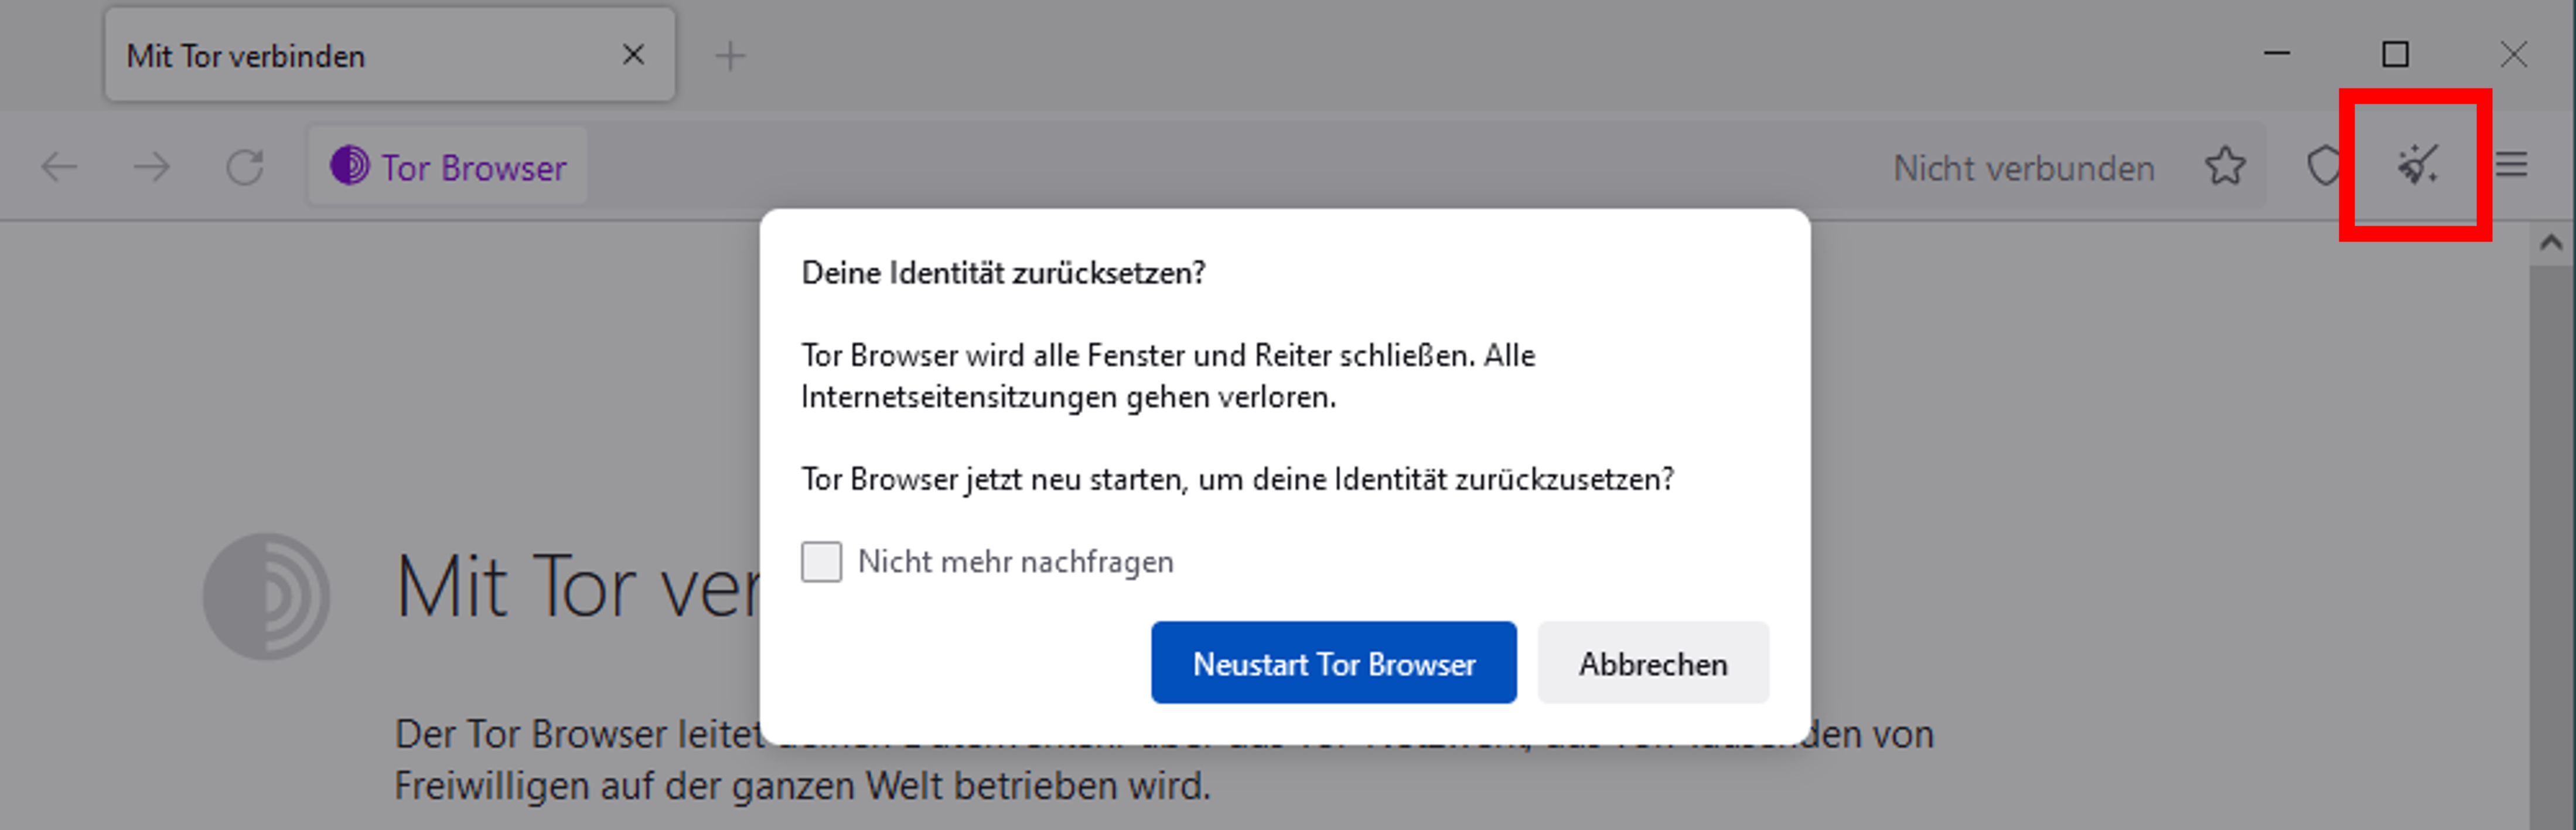
\includegraphics{bilder/tor-new-identity.png}}
	\caption{Funktion ``Neue Identität`` des Tor-Browsers}
	\label{img:tor-new-identity}
\end{figure}
Die in Abbildung \ref{img:tor-new-identity} gezeigte Funktion ``\textit{Neue Identität}`` ermöglicht es, alle aktuellen Tabs und Fenster zu schließen, sämtliche private Informationen wie Cookies und Verlauf zu löschen sowie die Verbindung mit dem Tor-Netzwerk neu zu konfigurieren.
%Für diesen Versuch: Tor Version 12.0.4 (64 Bit)

\subsubsection*{Chrome}
\label{subsubsection:methodik-vorbereitung-browserauswahl-chrome}

\subsubsection*{Brave}
\label{subsubsection:methodik-vorbereitung-browserauswahl-brave}

\subsection{Browsing Szenario}
\label{subsection:methodik-vorbereitung-browsing-szenario}
Im Falle der transparenten Versuchsdurchführung der Browser-Forensik werden eine Reihe von Aktivitäten definiert, die für jeden untersuchten Browser durchgeführt werden -- das sogenannte \textit{Browsing Szenario}.
In diesem Protokoll wird definiert, mit welchen Daten der Rechner kontaminiert werden soll.

Für diesen Versuch wurden ausschließlich Daten definiert, die nicht bereits vor Durchführung des Browsing-Szenarios auf dem Rechner zu finden sind. Beispielsweise sind die Zeichenketten ``twitter`` oder ``facebook`` bereits in vielen Windows-Standardanwendungen enthalten.

Folgende Schritte werden für diesen Versuch mit jedem Browser durchgeführt: 
\begin{enumerate}
\item  www.google.com aufrufen
	\begin{enumerate}[label*=\arabic*.]
	\item Alle Cookies akzeptieren 
	\item Google-Suche nach ``pfaffenhofen``
	\end{enumerate}
\item www.google.com aufrufen
	\begin{enumerate}[label*=\arabic*.]
	\item Cookies alle akzeptieren 
	\item Google-Suche nach ``nanoradar``
	\end{enumerate}
\item www.google.com aufrufen
	\begin{enumerate}[label*=\arabic*.]
	\item Cookies alle akzeptieren 
	\item Google-Suche nach ``mallofamerica``
	\item Auf Suchergebnis ``mallofamerica.com`` klicken
	\end{enumerate}
\item www.google.com aufrufen
	\begin{enumerate}[label*=\arabic*.]
	\item Cookies alle akzeptieren 
	\item Google-Suche nach ``mooserliesl``
	\item Auf Suchergebnis ``mooserliesl.de`` klicken
	\end{enumerate}
\item ``unitree.com`` über URL-Leiste öffnen
\item ``donaukurier.de`` über URL-Leiste öffnen
	\begin{enumerate}[label*=\arabic*.]
	\item Donaukurier Logo in neuem Tab öffnen
	\end{enumerate}
\item ``mail.google.com`` über URL-Leiste öffnen
	\begin{enumerate}[label*=\arabic*.]
	\item Mit google Account anmelden: 
			\begin{enumerate}[label*=\arabic*.]
			\item E-Mail = ``computerforensikvl@gmail.com``
			\item Passwort = ``Vorlesung23! ``
			\end{enumerate}
	\item Neue E-Mail schreiben:
			\begin{enumerate}[label*=\arabic*.]
			\item Empfänger: ``cas0597@thi.de`` und ``chs3702@thi.de``
			\item Betreff: ``Betrefftext``
			\item Mailinhalt: ``Mailinhalt``
			\end{enumerate}			
	\end{enumerate}
\end{enumerate}

Aus diesem Browsing-Szenario lassen sich die in Tabelle \ref{tab:pb-artefakte} dargestellten \textit{private Browsing Artefakte}, kurz \textit{PB Artefakte} ableiten. Dabei handelt es sich um Zeichenketten, die eindeutig einem Schritt im Browsing-Szenario zugeordnet werden können. Diese sind von zentraler Bedeutung in der Analysephase: Nur nach diesen Strings wird gesucht.

\begin{table}[h!]
\centering
\caption{Private Browsing Artefakte des Browsing-Szenarions}
\label{tab:pb-artefakte}
\begin{tabular}{|c|l|c|}
\hline
\textbf{Kategorie}           & \multicolumn{1}{c|}{\textbf{Private Browsing Artefakt}}                                      & \textbf{\begin{tabular}[c]{@{}c@{}}Schritt im\\  Browsing Szenario\end{tabular}} \\ \hline
\multirow{4}{*}{Suchbegriff} & ``pfaffenhofen``                                                                               & 1.2                                                                              \\ \cline{2-3} 
                             & ``nanoradar``                                                                                  & 2.2                                                                              \\ \cline{2-3} 
                             & ``mallofamerica``                                                                              & 3.2                                                                              \\ \cline{2-3} 
                             & ``mooserliesl``                                                                                & 4.2                                                                              \\ \hline
\multirow{4}{*}{URL}         & ``mooserliesl.de``                                                                             & 3.3                                                                              \\ \cline{2-3} 
                             & ``mallofamerica.com``                                                                          & 4.3                                                                              \\ \cline{2-3} 
                             & ``unitree.com``                                                                                & 5.                                                                               \\ \cline{2-3} 
                             & ``donaukurier.de``                                                                             & 6.                                                                               \\ \hline
Bild                         & \begin{tabular}[c]{@{}l@{}}0x89 0x50 0x4E 0x47 ...\\ (PNG als Hexadezimalwerte)\end{tabular} & 6.1                                                                              \\ \hline
\multirow{4}{*}{E-Mail}      & ``computerforensikvl@gmail.com``                                                               & 7.1.1                                                                            \\ \cline{2-3} 
                             & ``Vorlesung23! ``                                                                               & 7.1.2                                                                            \\ \cline{2-3} 
                             & ``cas0597@thi.de``                                                                             & 7.2.1                                                                            \\ \cline{2-3} 
                             & ``chs3702@thi.de``                                                                             & 7.2.1                                                                            \\ \hline
\end{tabular}
\end{table}


\subsection*{VM Konfiguration}
\label{subsection:methodik-vorbereitung-vmkonfiguration}

Eine empfohlene Herangehensweise bei Versuchen in Browser Forensik ist die Versuchsdurchführung in einer virtualisierter Umgebung. 
Neben der daraus entstehenden Reproduzierbarkeit und Transportierbarkeit der Ergebnisse, werden die Versuchsumgebungen der einzelnen Browser voneinander sowie von der Analyseumgebung getrennt. \cite{Muir.2019}
Als Virtualisierungssoftware wird für diesen Versuch die kostenlose Software \textit{Oracle VirtualBox VM} verwendet. Pro Browser existiert eine VM, auf der das Browsing Szenario durchgeführt wird. 

Alle VMs besitzen die gleiche, in Tabelle \ref{tab:vm-config} dargestellte Basiskonfiguration:
Zum Datenaustausch zwischen VM und Analyserechner wird ein \textit{gemeinsamer Order} eingerichtet. Somit werden beispielsweise ohne Kontaminierung der VM benötigte Programme auf dem Analyserechner heruntergeladen, in den gemeinsamen Ordner gelegt und offline auf der VM installiert.
Auf der VM werden zwei Werkzeuge der Sysinternal-Abteilung von Microsoft installiert, um in der Analysephase das Browserverhalten vollständig  untersuchen zu können: \textit{Process Monitor} ermöglicht die Aufzeichnung aller Prozessaktivitäten und \textit{Process Explorer} erweitert die Funktionen des Windows Task Managers. \cite{Markruss.05.06.2023, Markruss.05.06.2023b}
\begin{table}[h!]
\centering
\caption{Basiskonfiguration jeder VM des Versuchs}
\label{tab:vm-config}
\begin{tabular}{|l|l|}
\hline
\textbf{Betriebssystem}         & Windows 10 Pro, 64 Bit, Build: 19045.2006                                  \\ \hline
\textbf{Festplatte}             & 30 GB, VDI-Format, kein SSD Laufwerk                                       \\ \hline
\textbf{RAM}                    & 6 GB                                                                       \\ \hline
\textbf{Netzwerk}               & Netzwerkbrücke                                                             \\ \hline
\textbf{Verbindung zu Host-PC}  & Gemeinsamer Ordner                                                         \\ \hline
\textbf{Installierte Programme} & \begin{tabular}[c]{@{}l@{}}Process Monitor (Version 3.93)\\ Process Explorer (Version 17.04)\end{tabular} \\ \hline
\end{tabular}
\end{table}
Nachdem eine VM mit der Standardkonfiguration erstellt wurde, wird diese für jeden Browser dupliziert. Anschließend werden die Browser über den gemeinsamen Ordner in der entsprechenden VM installiert. Dazu wurden folgende Installationsverzeichnisse verwendet:
\begin{enumerate}
\item[\textbf{Firefox}] \texttt{C:$\backslash$Program Files$\backslash$Mozilla Firefox$\backslash$firefox.exe}
\item[\textbf{Tor}] \texttt{C:$\backslash$Program Files$\backslash$Tor Browser$\backslash$Browser$\backslash$firefox.exe}
\item[\textbf{Chrome}] ***TODO Christoph***
\item[\textbf{Brave}] ***TODO Christoph***
\end{enumerate}

\subsection*{Verwendete Software}
\label{subsection:methodik-vorbereitung-verwendetesoftware}
Neben der VM Konfiguration muss die Analyseumgebung vorbereitet werden. Als Analyseumgebung dient für diesen Versuch der Rechner, auf dem die VM läuft. (Windows 10 Home, 64 Bit, Build 19045.2965)
Zur Analyse der Browser werden diverse Tools benötigt.

\subsubsection*{Autopsy}
\label{subsubsection:methodik-vorbereitung-verwendetesoftware-autopsy}
Um erstellte Festplattenabbilder zu untersuchen wird das Tool \textit{Autopsy} verwendet. Dabei handelt es sich um ein open-source Tool, das auf der Sleuthkit-Bibliothek für die forensische Analyse von Dateisystemen basiert, diese mit zusätzlichen Funktionen erweitert und eine grafische Benutzeroberfläche für die forensische Analyse bietet. \cite{Autopsy.29.03.2023} 
%Für diesen Versuch verwendet: Version 4.20.0

\subsubsection*{Volatility}
\label{subsubsection:methodik-vorbereitung-verwendetesoftware-volatility}
Um Abbilder des Arbeitsspeichers zu untersuchen wird das open-source Framework \textit{Volatility} verwendet, das speziell darauf ausgerichtet ist, Informationen und Artefakte aus dem physischen oder virtuellen Arbeitsspeicher eines Computers zu extrahieren.
%Version: Volatility3, Version 2.4.1 (aktuellster Release)
Für diesen Versuch wird \textit{Volatility3} verwendet, eine 2020 veröffentlichte vollständige Neuschreibung des Volatility Frameworks.
Volatility basiert auf Plugins, welche spezifische Funktionen und Analysen für verschiedene Aspekte des Systems bereitstellen. \cite{GitHub.05.06.2023} Für diesen Versuch werden folgende Plugins verwendet:
\begin{itemize}
\item pslist	
\item yarascan		
\item memmap	 	
\item filescan
\item svcscan
\end{itemize}
Die genaue Beschreibung der Plugins sowie deren Zusammenhang ist in der Analysephase in Kapitel \ref{subsubsection:methodik-datenanalyse-uncommonlocations-analysemitvolatility} beschrieben.

\subsubsection*{Sonstige Tools}
\label{subsubsection:methodik-vorbereitung-verwendetesoftware-sonstigetools}
Tabelle \ref{tab:software-liste} listet zusammenfassend alle in diesem Versuch verwendeten Software-Programme, deren Verwendungszweck sowie Version auf.
Darunter befinden sich diverse zusätzliche unterstützende Tools, welche zur vollständigen Analyse benötigt werden.
\begin{table}[h!]
\centering
\caption{Vollständige Liste der verwendeten Software dieses Versuchs.}
\label{tab:software-liste}
\resizebox{\linewidth}{!}{
\begin{tabular}{|l|l|l|}
\hline
\multicolumn{1}{|c|}{\textbf{Software}} & \multicolumn{1}{c|}{\textbf{Verwendungszweck}}                                              & \multicolumn{1}{c|}{\textbf{Version}} \\ \hline
Oracle VirtualBox                       & Virtualisierung                                                                  & 7.0.8 r156879                         \\ \hline
Windows 10 Pro                          & VM Betriebssystem                                                                & Build: 19045.2006                     \\ \hline
Process Monitor                         & Aufzeichnung Prozessaktivitäten                                                  & 3.93                                  \\ \hline
Process Explorer                        & Darstellung der Eigenschaften aktueller Prozesse                                 & 17.04                                 \\ \hline
Autopsy                                 & Analyse Festplattenabbilder                                                      & 4.20.0                                \\ \hline
Volatiltiy                              & Analyse RAM-Abbilder                                                             & Volatility3 Version 2.4.1             \\ \hline
HxD                                     & Analyse Binärdateien in hexadezimaler und ASCII-Darstellung                      & 2.5.0.0                               \\ \hline
Notepad++                               & Analyse strukturierter Dateiformate, z.B. JSON, XML                              & 8.4.5                                 \\ \hline
Registry Explorer                       & Grafischer Oberfläche zur Untersuchung von Windows-Registry Hives                & 2.0.0.0                               \\ \hline
DB Browser for SQLite                   & Grafische Oberfläche zur Verwaltung und Untersuchung von SQLite-Datenbanken      & 3.12.2                                \\ \hline
sqldiff.exe                             & Befehlszeilen-Programm zur Anzeige von Unterschieden zwischen SQLite-Datenbanken & 3.42.0                                \\ \hline
ChromeCacheView                         & Einlesen von Chrome Cache-Dateien und visuelle Aufbereitung des Inhalts          & 2.46                                  \\ \hline
MZCacheView                             & Einlesen von Firefox Cache-Dateien und visuelle Aufbereitung des Inhalts         & 2.21                                  \\ \hline
FirefoxCache2                           & Erweitert MZCacheView, um Firefox ``index``-Cachedatei zu analysieren              & Commit b50ab4f                        \\ \hline
dejsonlz4                               & Dekomprimierung von .jsonlz4-Dateien                                             & Commit c4305b8                        \\ \hline
\end{tabular}
}
\end{table}


\section{Datensammlung}
\label{section:methodik-datensammlung}
In der Phase der Datensammlung werden alle potenziellen Beweismittel identifiziert und in einem forenisch analysierbaren Format gesichert \cite{Izzati.2022}.
Für diesen Versuch umfasst dies die Durchführung des Browsing Szenarios sowie die Sammlung von Ressoucen, die potentielle private Browsing Artefakte enthalten.

\subsection*{Process Monitor Logfiles}
\label{subsection:methodik-datensammlung-processmonitorlogfiles}
Um das Verhalten von privaten Browsingmodi möglichst vollständig zu untersuchen, schlagen Fayyad-Kazan et al. \cite{Fayyad.2021} vor, alle Aktivitäten des Browsers während Browsing-Szenarios aufzeichnen.
Dazu werden mit dem Tool Process Monitor alle Prozess-Aktivitäten zwischen zwei Zeitpunkten als \textit{Process Monitor Logfile} (PML) oder CSV-Datei gespeichert. \cite{Fayyad.2021, Rochmadi.2017}
Die PML-Dateien werden mithilfe des gemeinsamen Ordners auf den Analyserechner transportiert.

\subsection*{Speicherabbilder}
\label{subsection:methodik-datensammlung-speicherabbilder}
Eine der Hauptaufgaben eines Computer-Forensischen-Ermittlers ist die Erstellung und Analyse von direkten Kopien der Speichermedien des untersuchten Rechners. \cite{Hassan.2019}
Im Falle der Browserforensik werden Abbilder der Festplatten und des Arbeitsspeicher erstellt und analysiert.

\paragraph*{Festplatten-Image}
Da in diesem Versuch die Festplatten virtualisiert werden, wird ein Abbild aus einem sogenannten \textit{VM-Snapshot} gewonnen, eine Momentaufnahme der virtuellen Maschine. \cite{Oracle.2020} 
VM-Snapshots können \textit{aufgetaut} werden, wodurch der Zeitpunkt der Momentaufnahme des Betriebssystems wiederhergestellt wird.
Bei Oracle VirutalBox kann ein VM Snapshot über die grafische Oberfläche erstellt werden.
Durch den Snapshot wird ein \textit{Virtual Disk Image}, eine VDI-Datei, im Snapshot-Ordner der VM erzeugt. Diese Laufwerksdatei enthält nur differentielle Daten zum vorherigen Snapshot.
Um aus den differentiellen Daten ein vollständiges Festplatten-Image zu erzeugen, muss ein \textit{vollständiger Klon} des Snapshots erstellt werden. Die VDI-Datei der geklonten VM entspricht einem vollständigem Abbild der Festplatte zum Zeitpunkt des durchgeführten Snapshots.

Da Autopsy nicht das VDI-Format unterstützt, müssen die Laufwerksdateien der geklonten Snapshots in ein das generische \textit{Image}-Format (.img) umgewandelt werden.
Durch Nutzung des VirtualBox Befehlszeilen-Tool \textit{vboxmanage} wird mit dem Befehl \texttt{vboxmanage clonehd <VDI\_File>.vdi <IMG\_File>.img --format raw} die VDI-Datei ein eine IMG-Datei umgewandelt.
Um ein Festplatten-Image in Autopsy einzulesen, wird ein neuer \textit{Fall} (engl. Case) erstellt. Das Einlesen eines ca. 30 GB großen Festplatten-Images dauerte mit allen aktivierten Autopsy-Plugins zwischen 5 und 7 Stunden.

\paragraph*{RAM-Dump}
Ein \textit{RAM-Dump} erfasst den Zustand des Arbeitsspeichers, einschließlich der im Speicher befindlichen Daten, Programme und Prozesse zu einem bestimmten Zeitpunkt \cite{TILT.25.03.2023}.
VirtualBox empfiehlt, Abbilder des RAMs ebenfalls über das vboxmanage Befehlszeilen-Tool durchzuführen.
Im Unterschied zu Festplatten-Images können RAM-Dumps nur im angeschalteten Zustand der virtellen Maschine mithilfe des Befehls \texttt{vboxmanage debugvm <VM Name> dumpvmcore --filename <RAM Dump Dateiname>.elf} durchgeführt werden. RAM-Dumps im .elf Format können direkt vom Analysetool Volatility innerhalb weniger Minuten eingelesen werden.		

\paragraph*{Zeitpunkte zur Datensammlung}
Wichtig für die Qualität der Versuchsergebnisse sind die Zeitpunkte während des Browsing Szenarios zum Sammeln der Daten.
In der Literatur wählen die Autoren meist ohne Begründung Zeitpunkte zur Datensammlung \cite{Sajan.2021, Nalawade.2016, Montasari.2015, Satvat.2014, Said.2011, Aggarwal.2010}.
Dieses Problem haben Muir, Leimich und Buchanan erkannt und Zeitpunkte zur Datensammlung vorgeschlagen, um das Browserverhalten während des Browsing-Szenarios vollständig analysieren zu können \cite{Muir.2019}. Wie in Abbildung \ref{img:zeitpunkte-datensammlung} dargestellt, wurde sich an diesen Zeitpunkten für diesen Versuch orientiert.
\begin{figure}[h!]
	\caption{Zeitpunkte zur Datensammlung während der Versuchsdurchführung nach \cite{Muir.2019}}
	\label{img:zeitpunkte-datensammlung}
	\centering
	\small
	\centerline{\resizebox{\linewidth}{!}{\input{bilder/datensammlung-zeitpunkte-Latex.pdf_tex}}}
\end{figure}

Der erste RAM-Dump sowie der erste VM-Snapshot nach der Browser-Installation, vor Beginn des Browsing-Szenarios, dienen als Baseline für die Analyse, da in diesen Speicherabbildern kein PB Artefakt gefunden werden darf.
Nachdem der private Modus im Browser geöffnet wird und bevor das Browsing Szenario beginnt, wird die Aufnahme des ersten Process Monitor Logfiles gestartet. Um ausschließlich Schreiboperationen aufzuzeichnen, die auf das private Browsing zurückzuführen sind, wird die Aufzeichnung erst nach dem erstmaligen Öffnen des Browsers im privaten Modus gestartet.
Nach Durchführung des Browsing-Szenarios, während der Browser noch geöffnet ist, wird die Aufnahme des ersten Process Monitor Logfiles gestoppt. Weiterhin wird ein zweiter RAM-Dump sowie VM-Snapshot erstellt. Anschließend wird das eine zweite Process Monitor Aufzeichnung gestartet. 
Nachdem der Browser geschlossen wurde, wird die Aufzeichnung des zweiten Process Monitor Logfiles beendet. Somit enthält das zweite Logfile wird alle Prozessaktivitäten vom Schließen der Browsers. Zusätzlich wird ein dritter RAM-Dump sowie  VM-Snapshot erstellt. 
Nach Herunterfahren der VM wird ein vierter VM-Snapshot erstellt, der für die für Post-Mortem Analyse relevant ist.

\paragraph*{Sonderfälle}
Dieses Vorgehen zur Datensammlung wird bei allen Browsern durchgeführt. Einzig der Tor-Browser weicht davon ab. Um die ``Neue Identität``-Funktion des Tor-Browsers zu berücksichten, werden zusätzlich Daten vor und nach der Erstellung einer ``Neuen Identiät`` gesammelt. Wie in Abbildung \ref{img:zeitpunkte-datensammlung-tor} dargestellt, umfasst dies einen zusätzlichen RAM-Dump sowie VM-Snapshot und ein weiteres Process Monitor Logfile.
\begin{figure}[h!]
	\caption{Zeitpunkte zur Datensammlung während der Versuchsdurchführung für den Tor-Browser}
	\label{img:zeitpunkte-datensammlung-tor}
	\centering
	\small
	\centerline{\resizebox{\linewidth}{!}{\input{bilder/datensammlung-zeitpunkte-tor-Latex.pdf_tex}}}
	\label{fig:jes}
\end{figure}

Bei Durchführung des Browsing-Szenarios für den Firefox-Browser wurde nach erstmaligem Öffnen des Browsers automatisch die Firefox Datenschutz-Webseite \texttt{https://www.mozilla.org/\\
de/privacy/firefox/} im nicht-privaten Modus geöffnet. 

\section{Datenanalyse}
\label{section:methodik-datenanalyse}
Nachdem die Daten in Form von Process Monitor Logfiles und Festplatten- sowie RAM-Speicherabbildern gesammelt wurden, wird nach den PB Artefakten aus Tabelle \ref{tab:pb-artefakte} in Kapitel \ref{subsection:methodik-vorbereitung-browsing-szenario} gesucht. 
Die gesammelten Daten des Versuchs werden zur Vereinfachung der Analyse in drei Kategorien aufgeteilt: \textit{Common Locations}, \textit{Uncommon Locations} sowie \textit{Registry}.

\subsection{Common Locations}
\label{subsection:methodik-datenanalyse-commonlocations}
Die sogenannten \textit{Common Locations} beziehen im Zusammenhang der Browserforensik auf die standardmäßigen Verzeichnisse eines Browsers auf der Festplatte, beispielsweise Ordner von Browsern zur Verwaltung von Nutzerdaten.
Untersucht werden Common Locations mittels \textit{Whitebox-Analyse}, 
wodurch der Fokus darauf liegt, das System vollständig zu verstehen und alle relevanten Beweise zu sammeln. \cite{Bonetti.2014}

Bei diesem Versuch werden die Speicherorte über die Schreiboperationen der Process Monitor Logfiles identifiziert.
Anschließend wird für jede Datei in den Speicherorten geprüft, ob PB Artefakte enthalten sind.
Dazu sind zwei Schritte notwendig:
\begin{enumerate}
\item \textbf{Dateiextraktion}: Extrakion der Datei aus dem Speicherabbild. Wenn die Datei nicht mehr vorhanden ist, werden dazu ggf. Tools zur Dateiwiederherstellung benötigt.
\item \textbf{Dateianalyse}: Um zu überprüfen ob die Datei PB Artefakte enthält, werden ggf. Tools für spezielle Dateiformate benötigt, beispielsweise Dekomprimierungstools.
\end{enumerate}

\paragraph*{Identifikation der Common Locations}
Um die gängigen Browserpfade und -dateien zu identifizieren, werden die in den Process Monitor Logfiles aufgezeichneten Schreibaktivitäten der Browserprozesse ausgewertet.

Dazu wird jedes Logfile mit dem Process Explorer eingelesen. Anschließend werden die Aktivitäten gefiltert.
\begin{figure}[h!]
	\centerline{\resizebox{0.7\linewidth}{!}{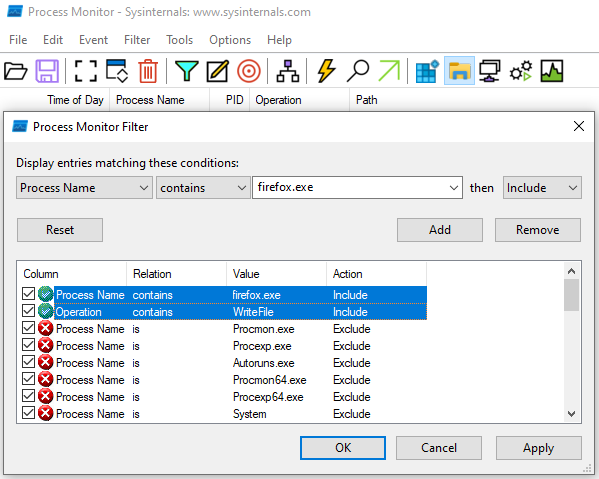
\includegraphics{bilder/process-monitor-filter.png}}}
	\caption{Process Monitor Filter für Datei-Schreiboperationen}
	\label{img:procmon-writefile-filter}
\end{figure}
Wie in Abbildung \ref{img:procmon-writefile-filter} dargestellt, werden dazu ausschließlich die Option ``File System Activity`` ausgewählt.
Anschließend wird als Prozessname der Browserprozess gesetzt:
\begin{itemize}
\item \textbf{Firefox}: firefox.exe
\item \textbf{Tor-Browser}: firefox.exe und tor.exe
\item \textbf{Chrome}: chrome.exe
\item \textbf{Brave}: brave.exe
\end{itemize}
Da PB Artefakte nur über Schreiboperationen entstehen können, wird als Prozessoperation ``WriteFile`` gesetzt.
Die gefilterte Logfile wird als CSV exportiert, um sie dann in Excel zu öffnen und irrelevante Spalten sowie Duplikate zu löschen.
Die geschriebenen Dateien werden anschließend browserspezifisch gruppiert.

\paragraph*{Prüfung auf PB Artefakte}
Nachdem die geschriebenen Browserdateien identifiziert und gruppiert wurden, wird für jede Datei geprüft, ob PB Artefakte enthalten sind. Folgende, in Abbildung \ref{img:dateiextraktion-und-analyse} dargestellte Schritte sind zur Dateiextraktion und Dateianalyse notwendig:
Die Datei befindet sich entweder im entsprechenden Festplatten-Image oder ist im RAM-Dump gespeichert. 
Wenn die Datei nicht mit Autopsy aus dem Festplatten-Image extrahiert werden kann und sich der Dateiname in der Ausgabe des Volatiltiy Plugins \textit{filescan} (\texttt{vol.py -f ram\_dump.img windows.filescan > filescan.txt}) befindet, wird diese mit dem Volatility Plugin \textit{dumpfiles} aus dem RAM extrahiert.
Wenn auch dies nicht möglich ist und es sich um eine temporäre Datei (.tmp) handelt, wird versucht die enstprechende nicht-temporäre Datei zu extrahieren. 
Im Falle der Datei ``some-file.json.tmp`` wird beispielsweise geprüft, ob die Datei ``some-file.json`` existiert.
Nachdem die Datei extrahiert wurde und ggf. mit einem Tool zu Analyse vorberarbeitet wurde, wird geprüft, ob die Datei PB Artefakte enthält.
\begin{figure}[h!]
	\centering
	\small
	\centerline{\resizebox{\linewidth}{!}{\input{bilder/process_monitor_to_exce-Latexl.pdf_tex}}}
	\caption{Vorgehen zur Dateiextration und -analyse}
	\label{img:dateiextraktion-und-analyse}
\end{figure}

\paragraph*{SQLite-Datenbänke}
\label{subsubsection:methodik-datenanalyse-commonlocations-sqlitedbs}
Eine besondere Rolle unter den Common Locations bei Browsern nehmen SQLite Datenbänke ein. 
Sie speichern und verwalten Nutzerinformationen, wie Lesezeichen, Browserverlauf, Caches, Cookies in Datenbankdateien zu speichern, ohne einen separaten Datenbankserver zu benötigen.

Wie in Abbildung \ref{img:dateiextraktion-und-analyse-sqlite} dargestellt, erfolgt die Dateiextraktion analog zur Vorgehensweise bei den Schreiboperationen der Process Monitor Logfiles: Um die SQLite Datenbänke zu analysieren wird jede Datenbank mit der gleichen Datenbank aus dem vorherigem Snapshot mithilfe des Befehlszeilentools \textit{sqldiff.exe} (\texttt{sqldiff.exe database1.sqlite database2.sqlite}) verglichen. Die Inhaltsunterschiede werden für jede Datei in jedem Snapshot untersucht und in einer Excel Tabelle festgehalten.
Datenbankänderungen einer SQLite-Datei werden zuerst im \textit{Write-Ahead Log}, kurz \textit{WAL}, vorübergehend protokolliert. 
Um potentielle PB Artefakte zu berücksichtigen, wird der WAL mithilfe der sqlite3 Befehlszeile (\texttt{sqlite3> PRAGMA wal\_checkpoint;}) in die SQLite Hauptdatenbank geschrieben.
\begin{figure}[h!]
	\centering
	\small
	\centerline{\resizebox{\linewidth}{!}{\input{bilder/sqlite-methodology-Latex.pdf_tex}}}
	\caption{Vorgehen zur Dateiextration und -analyse von SQLite Datenbanken}
	\label{img:dateiextraktion-und-analyse-sqlite}
\end{figure}

\subsection{Uncommon Locations}
\label{subsection:methodik-datenanalyse-uncommonlocations}
\textit{Uncommon Locations} beziehen sich auf Verzeichnisse, die nicht zu den gängigen Speicherorten gehören. 
Bei Festplatten-Images handelt es sich dabei meist um Dateien des Betriebssystems oder andere Festplattenbereiche, wie beispielsweise unallokierte Speicherbereiche oder der Arbeitsspeicher.
Uncommon Locations werden ohne Vorwissen über das Browserverhalten sowie ohne Vorverarbeitung der Dateien mithilfe der \textit{Blackbox-Analyse} untersucht \cite{Bonetti.2014}:
Im Kontext der Browser Forensik werden dazu Stringsuchen nach PB Artefakten über die gesamten Speicherabbilder durchgeführt.
Dies ist nur durch Unterstützung mit Forensik-Tools möglich. Somit wird bei der Analyse der Uncommon Locations in die Vollständigkeit der Tools vertraut.

\subsubsection*{Analyse mit Autopsy}
\label{subsubsection:methodik-datenanalyse-uncommonlocations-analysemitautopsy}
Bei den Uncommon Locations wird Autopsy als forensisches Werkzeug zur Analyse der Festplatten-Images verwendet.
Dazu wird eine Stichwortsuche mit den in Tabelle \ref{tab:pb-artefakte} definierten PB Artefakten über das gesamte eingelesene Festplatten-Image durchgeführt.

Autopsy bietet dazu die in Abbildung \ref{img:autopsy-keywordsuche} dargestellte Funktion zur Suche nach Strings, Teilstrings oder regulären Ausdrücken in Dateinamen und Dateiinhalten an.
\begin{figure}[h!]
	\centerline{\resizebox{0.85\linewidth}{!}{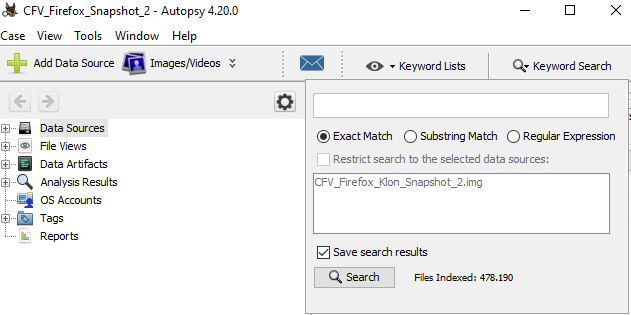
\includegraphics{bilder/autopsy-search.png}}}
	\caption{Autopsy Funktion zur Stichwortsuche}
	\label{img:autopsy-keywordsuche}
\end{figure}

Zusätzlich kategorisiert Autopsy automatisch die Dateien eines Festplatten-Images. Für diesen Versuch sind folgende Dateikategorien von Interesse:
\begin{itemize}
\item Web Bookmarks
\item Web Cookies
\item Web History
\item Web Categories
\end{itemize}

\subsubsection*{Analyse mit Volatility}
\label{subsubsection:methodik-datenanalyse-uncommonlocations-analysemitvolatility}
Bei der Analyse des Arbeitsspeichers als Uncommon Location ist es kritisch, dass ein gefundener String eindeutig einem Browserprozess zugeordnet werden kann. 

In der Literatur wird der Arbeitsspeicher oft unzureichend durch eine Stichwortsuche im RAM-Dump analysiert, der als Binärdatei in einem Hexadezimaleditor geöffnet ist. \cite{Rochmadi.2017, Md.2018, Montasari.2015}
Wie beispielhaft in Abbildung \ref{img:textfile-ram-artifact} gezeigt, wird ein String, der in einer Textdatei auf dem Desktop gespeichert ist ebenfalls im Hexadezimaleditor HxD angezeigt, obwohl kein Browsing Szenario durchgeführt wurde.
\begin{figure}[h!]
	\centering
	\subcaptionbox{String in Textdatei}{
\includegraphics[width=0.30\textwidth]{bilder/ram-editor1.png}}%
	\hfill
	\subcaptionbox{String als Hexadezimalwert in RAM-Dump (geöffnet mit HxD)}{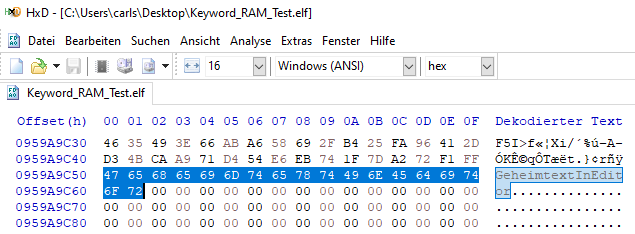
\includegraphics[width=0.65\textwidth]{bilder/ram-editor2.png}}%
	\caption{Negativbeispiel für gefundenes RAM-Artefakt}
	\label{img:textfile-ram-artifact}  
\end{figure}

Um einen im RAM gefundenen String einem Browserprozess zuordnen zu können, wird deshalb das forensiche Analysetool Volatility mit dem PlugIn \textit{Yarascan} verwendet.
Mithilfe sogenannter \textit{Yara-Regeln} (engl. Yararules) wird nach bestimmten Mustern im Arbeitsspeicher gesucht.
Die für diesen Versuch verwendeten Yara-Regeln entsprechen den Strings der PB Artefakte in Tabelle \ref{tab:pb-artefakte}. Zusätzlich sucht eine Regel nach HTML-Fragmenten, die eindeutig einer besuchten Seite des Browsing-Szenarios zuzuordnen sind. \cite{Said.2011}
Alle verwendeten Yara-Regeln sind im Anhang X (TODO!) aufgelistet.
Um den RAM-Dump nach den Yara-Regeln zu durchsuchen, wird folgender Befehl ausgeführt: \texttt{vol.py -f ram\_dump.img windows.vadyarascan --yara-file yara\_rules.yara > yarascan.txt}
Nachdem der RAM-Dump nach den Regeln durchsucht wurde, gibt die Yarascan-Ausgabe für jeden gefundenen String die PID des Prozesses, in dem der String gefunden wurde, sowie die virtuelle Speicheradresse des gefundenen Strings an.

Wie in Abbildung \ref{img:volatility-plugins} dargestellt, wird davon ausgehend mit dem Plugin \textit{pslist} (\texttt{vol.py -f ram\_dump.img windows.pslist --pid <PID> > pslist.txt}) der Prozessname der PID ermittelt, in dem der String gefunden wurde.
\begin{figure}[h!]
	\centering
	\small
	\centerline{\resizebox{\linewidth}{!}{\input{bilder/yarascan_plugin_tree-Latex.pdf_tex}}}
	\caption{Abhängigkeiten der verwendeten Volatility-Plugins yarascan, pslist und memmap}
	\label{img:volatility-plugins}
\end{figure}
Oft ist bei einem gefundenen String von Interesse, ob in den Speicheradressen vor und nach dem Treffer weitere Zusammenhänge erkennbar sind.
Mithilfe des Plugins \textit{memmap} (\texttt{vol.py -f ram\_dump.img windows.memmap --pid <PID> > memmap.txt}) wird die Abbildung der virtuellen Speicheradressen eines Prozesses auf die Byte-Offsets der extrahierten Speicherseite des Prozesses ermittelt.
Diese Seite kann mithilfe des ``--dump`` Flags extrahiert werden: \texttt{vol.py -f ram\_dump.img -o $\backslash$dump\_dir$\backslash$ windows.memmap --pid <PID> --dump}.
In einem Hexadezimaleditor, wie HxD, kann der String-Treffer anhand des ermittelten Byte-Offsets in der Speicherseite untersucht werden.

\subsection{Registry}
\label{subsection:methodik-datenanalyse-registry}
Die letzte Kategorie analysierter Daten umfasst die Artefakte der Registry.
Diese zählen sowohl zu den Common als auch Uncommon Locations und werden deshalb eigene Kategorie aufgeführt.

\paragraph*{Common Locations}
%*** TODO: Common location: Shellactivities Key ***
%	existiert nicht mehr --> Nicht mehr vorhanden in aktueller Version (Verweis auf E-Mail)
Als Teil der Common Locations werden die Registry-Aktivitäten in den Process Monitor Logfiles analysiert.
\begin{figure}[h!]
	\centerline{\resizebox{0.7\linewidth}{!}{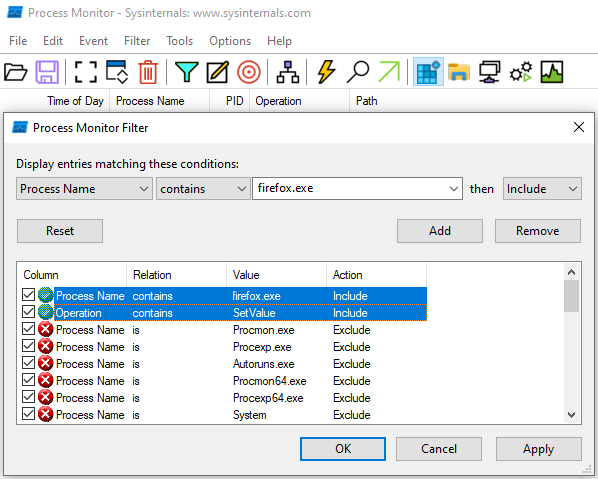
\includegraphics{bilder/process-monitor-filter-registry.png}}}
	\caption{Process Monitor Filter für Registry-Schreiboperationen}
	\label{img:procmon-setvalue-filter}
\end{figure}
Wie in Abbildung \ref{img:procmon-setvalue-filter} gezeigt, wird zunächst die Logfile nach ``Registry Activity`` sowie Einträgen mit der Operation ``SetValue`` sowie dem Browser-Prozessnamen gefiltert.
Als CSV Datei wird das Logfile in Excel weiter verarbeitet, indem Duplikate gelöscht werden und die geschriebenen Registry Keys browserspezifisch gruppiert werden.
	
\paragraph*{Uncommon Locations}
Unter Betrachtung als Uncommon Location werden alle Registry Hives in jedem Festplatten-Image mit dem Registry Explorer untersucht.
Dabei wird zwischen Hives zur Speicherung von Systemeinstellungen (System-Hives) und individuellen Benutzerkonfigurationen (User-Hives) unterschieden. Diese in Tabelle \ref{tab:windows-registry-hives} dargestellten Hives werden von Windows beim Start geladen und dienen Systemkomponenten und Anwendungen als Quelle für Einstellungen und Informationen. \cite{Haircutfish.04.11.2022}
Zur Analyse wird jeder Hive aus den Fesplatten-Images extrahiert und in eine Registry Explorer Sitzung geladen und eine Stringsuche nach PB Artefakten durchgeführt.

\begin{table}[h!]
\centering
\caption{Windows Registry Hives}
\label{tab:windows-registry-hives}
\resizebox{\linewidth}{!}{
\begin{tabular}{lllll}
\cline{1-2}
\multicolumn{2}{|c|}{\textbf{System-Hives (C:\textbackslash{}\textbackslash{}Windows\textbackslash{}\textbackslash{}System32\textbackslash{}\textbackslash{}Config)}} &  &  &  \\ \cline{1-2}
\multicolumn{1}{|l|}{\textbf{Dateiname}}             & \multicolumn{1}{l|}{\textbf{Inhalt}}                                                                           &  &  &  \\ \cline{1-2}
\multicolumn{1}{|l|}{\textit{DEFAULT}}               & \multicolumn{1}{l|}{Standardkonfigurationseinstellungen für neue Benutzerprofile.}                             &  &  &  \\ \cline{1-2}
\multicolumn{1}{|l|}{\textit{SAM}}                   & \multicolumn{1}{l|}{Sicherheitskontensdaten, einschließlich der Benutzerkonten und deren Kennwörter.}          &  &  &  \\ \cline{1-2}
\multicolumn{1}{|l|}{\textit{SECURITY}}              & \multicolumn{1}{l|}{Sicherheitsinformationen für die Zugriffssteuerung und Authentifizierung.}                 &  &  &  \\ \cline{1-2}
\multicolumn{1}{|l|}{\textit{SOFTWARE}}              & \multicolumn{1}{l|}{Konfigurationsdaten für installierte Software und Anwendungen.}                            &  &  &  \\ \cline{1-2}
\multicolumn{1}{|l|}{\textit{SYSTEM}}                & \multicolumn{1}{l|}{Systemkonfigurationseinstellungen und Gerätetreiberinformationen.}                         &  &  &  \\ \cline{1-2}
                                                     &                                                                                                                &  &  &  \\ \cline{1-2}
\multicolumn{2}{|c|}{\textbf{User-Hives (C:\textbackslash{}\textbackslash{}Users\textbackslash{}\textbackslash{}\textless{}username\textgreater{})}}                  &  &  &  \\ \cline{1-2}
\multicolumn{1}{|l|}{\textbf{Dateiname}}             & \multicolumn{1}{l|}{\textbf{Inhalt}}                                                                           &  &  &  \\ \cline{1-2}
\multicolumn{1}{|l|}{\textit{NTUSER.DAT}}            & \multicolumn{1}{l|}{Individuelle Einstellungen und Konfigurationen für den angemeldeten Benutzer}              &  &  &  \\ \cline{1-2}
\multicolumn{1}{|l|}{\textit{USRCLASS.DAT}}          & \multicolumn{1}{l|}{Dateizuordnungen und Registrierungseinstellungen für den angemeldeten Benutzer}            &  &  &  \\ \cline{1-2}
\end{tabular}
}
\end{table}
	


	
	\chapter{Ergebnisse}

*** TODO ***

\section{Firefox}

Im nachfolgenden Abschnitt werden die Ergebnisse der Datenanalyse für den Webbrowser Firefox detailliert beschrieben. Die Analyse ist in drei Hauptkategorien unterteilt: Common Locations, Uncommon Locations und Registry.

\subsection*{Common Locations}

Zunächst werden die standardmäßigen Speicherorte für Browserartefakte nach potentiellen privaten Browsing Artefakten untersucht. Diese Common Locations beziehen sich ausschließlich auf Dateien, die auf die Festplatte geschrieben werden. In diesem Versuch wird gemäß Methodik in Kapitel X (TODO!) zwischen Schreiboperationen aus den Process Monitor Logfiles und SQLite Datenbänken zur Verwaltung von Nutzerdaten unterschieden.

\subsubsection*{Process Monitor WriteFile Operations}

Gemäß Versuchsdurchführung in Abbildung X (TODO!) wurden für Firefox mit dem Process Monitor Tool zwei Logfiles erstellt. Diese Dateien enthalten alle aufgezeichneten Prozessaktivitäten während und nach dem Browsing Szenario.
Zunächst werden die beiden Logfiles gemäß Methodik in Kapitel X (TODO!) in Excel aufbereitet. 
Im Anhang X (TODO!) ist dazu eine Tabelle mit allen in den gefilterten Logfiles identifizierten Dateien aufgeführt.
Dabei wurde für jede Datei vermerkt
ob und wie sie wiederherstellbar war, mit welchem Tool die Datei analysiert wurde und ob PB Artefakte enthalten sind.

Abbildung X (TODO!) zeigt diese Tabelle in reduzierter Darstellung.
Dazu wurden ausschließlich wiederherstellbare Dateien aufgeführt. 
Die Dateien wurden in die fünf Kategorien "Cache", "datareporting", "Sessionstore-Backup" und "Sonstige Dateien" eingeordnet.
Für jede Datei wurde vermerkt, ob in der entsprechenden Logfile PB Artefakte geschrieben wurden.
Dies trifft für keine der identifizierten Dateien zu.
\begin{figure}[h!]
	\resizebox{\linewidth}{!}{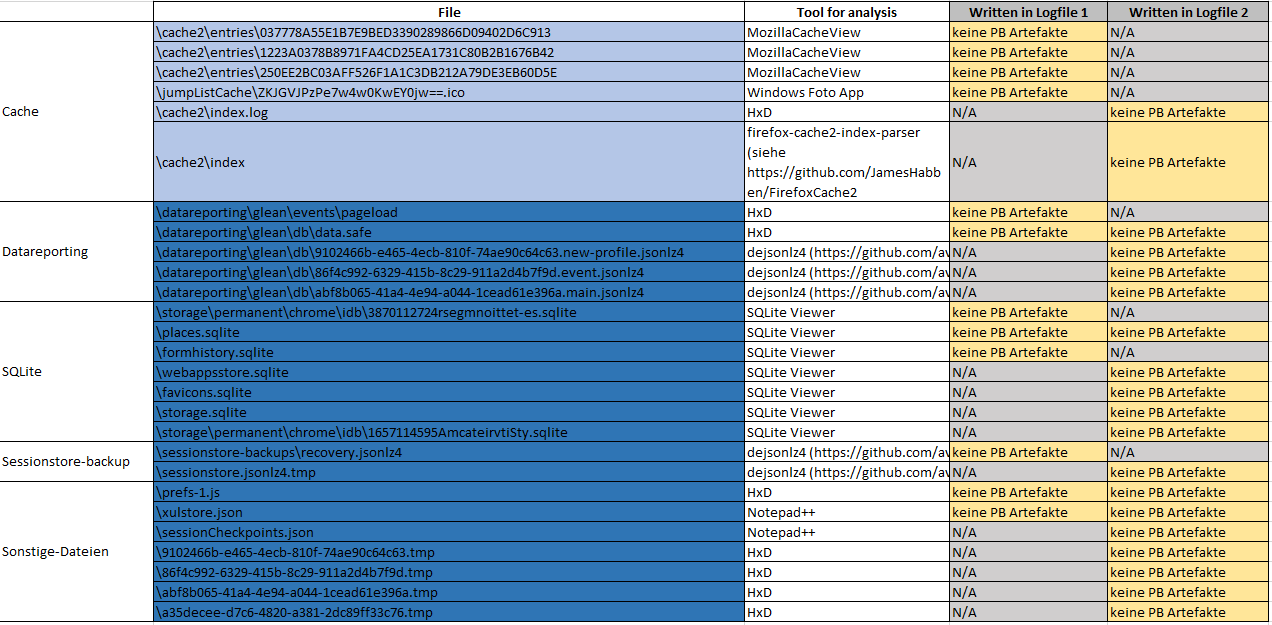
\includegraphics{bilder/firefox-tabelle-logfile1vlogfile2-reduced.png}}
%	\label{...}
	\caption{Tabelle mit wiederherstellbaren Dateien: Logfile 1 vs. Logfile 2}
\end{figure}

Bei detaillierter Untersuchung der Dateien, können zwei Pfade identifiziert werden, in die Firefox während des Versuchs Dateien schreibt. Nur die Dateien in der Cache Kategorie sind im Local Pfad gespeichert.
\begin{itemize}
\item[\textbf{Local}] \texttt{C:$\backslash$Users$\backslash$<User>$\backslash$AppData$\backslash$Local$\backslash$Mozilla$\backslash$Firefox$\backslash$Profiles$\backslash$<Profile>.default-release$\backslash$}
\item[\textbf{Roaming}] \texttt{C:$\backslash$Users$\backslash$<User>$\backslash$AppData$\backslash$Roaming$\backslash$Mozilla$\backslash$Firefox$\backslash$Profiles$\backslash$<Profile>.default-release$\backslash$}
\end{itemize}
In Tabelle X (TODO!) sind die Dateien je nach Speicherort "Local" (Hellblau) oder "Roaming" (Dunkelblau) entsprechend eingefärbt. 

\paragraph*{Cache}

Firefox verwendet den Cache, um Webseiten und deren Ressourcen temporär lokal zu speichern. Dadurch können wiederholte Anfragen an den Server vermieden und die Ladezeiten verringert werden. Die Inhalte dieser Dateien sind binär.
Die Dateien im Format \texttt{$\backslash$cache2$\backslash$entries$\backslash$<ID>} werden dem Cache zugeordnet und im Local Pfad gespeichert.
% https://www.techguy.org/threads/what-exactly-is-in-firefoxs-cache2-folder.1221567/
Wie in Kapitel X beschrieben, können diese Dateien mit dem Tool MZCacheView eingelesen werden.
Wie in Abbildung X gezeigt, konnten im Cache-Ordner im zweiten Snapshot drei JSON Dateien identifiziert werden. Dabei handelt es sich um Zertifikatsdateien, die von der "One Certificate Revocation List" stammen, ein Mechanismus von Firefox zur Überprüfung von Zertifikaten. In keinem der Zertifikate konnten mit HxD private Browsing Artefakte oder besuchte Seiten gefunden werden.
Weiterhin befindet sich im Cache das HTML-Dokument der Firefox Datenschutzseite, welche sich beim ersten Start des Browsers automatisch öffnete. % TODO: Siehe Kapitel X
Weitere Cache Dateien konnten in keinem Snapshot gefunden werden.
\begin{figure}[h!]
	\resizebox{\linewidth}{!}{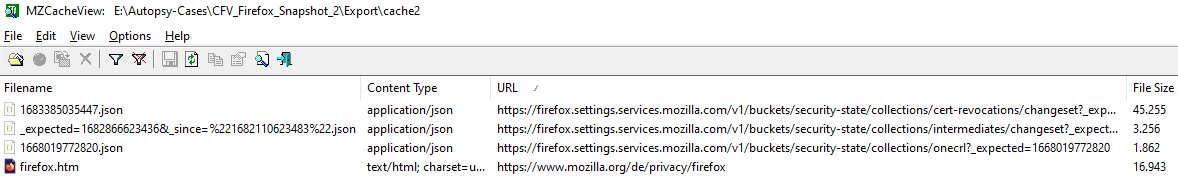
\includegraphics{bilder/firefox-cache.png}}
%	\label{...}
	\caption{Tabelle mit wiederherstellbaren Dateien: Logfile 1 vs. Logfile 2}
\end{figure}
Die Indexdatei \texttt{$\backslash$cache2$\backslash$index} dient als Datenbank im Cache. Sie ermöglicht dem Firefox-Browser, schnell auf die zwischengespeicherten Ressourcen zuzugreifen und diese effizient zu verwalten. Sowohl mit HxD als auch dem Tool FirefoxCache2 konnten keine PB Artefakte identifiziert werden.
Schließlich enthält die Datei \texttt{$\backslash$jumpListCache$\backslash$ZKJGVJPzPe7w4w0KwEY0jw==.ico} ein $64x64$ Pixel großes Mozilla Logo. Dieses Logo ist keinem Schritt aus dem Browsing Szenario zuzuordnen


\paragraph*{Datareporting}
Dateien im Ordner \texttt{$\backslash$datareporting$\backslash$glean$\backslash$db} sind Teil des Glean-Systems, das für die Sammlung von Telemetriedaten und deren Übermittlung an Mozilla verwendet wird. 
% https://github.com/mozilla/glean
Die Datei \texttt{data.safe.bin} enthält verschlüsselte und anonyme Informationen über die Nutzung des Browsers. In HxD konnten keine keine PB Artefakte gefunden werden
Dateien im Foremat \texttt{$\backslash$datareporting$\backslash$glean$\backslash$db$\backslash$<Profilname>.new-profile.jsonlz4} speichern Informationen über das Firefox-Profil, das von Glean verwendet wird. Wie in Kapitel X beschrieben, lassen sich Dateien, im proprietären \textit{jsonlz4}-Format mit dem Tool dejsonlz4 dekomprimieren. Die entstandene JSON Datei wird mit dem Notepad++ JSON Plugin untersucht. Dabei konnten keine PB Artefakte gefunden werden.

\paragraph*{Sessionstore}
Die Datei \texttt{$\backslash$sessionstore-backups$\backslash$recovery.jsonlz4} enthält eine Sicherungskopie der vorherigen Sitzung. Sie wird erstellt, wenn der Firefox-Browser nach einem Absturz oder einem unerwarteten Beenden neu gestartet wird." % https://support.mozilla.org/de/questions/1221836
Jefferson Scher entwickelte ein Online-Tool zur Analyse von \textit{Sessionstore-Backup} Dateien.
% https://www.jeffersonscher.com/ffu/scrounger.html)
In der Sitzungswiederherstellung konnten wie in Abbildung X gezeigt lediglich die automatisch geöffnete Seite über Firefox Datenschutzhinweise identifiziert werden.
\begin{figure}[h!]
	\resizebox{\linewidth}{!}{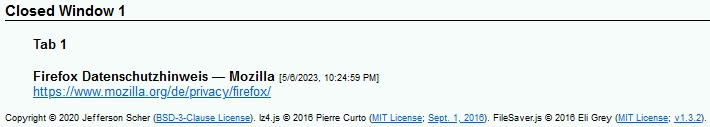
\includegraphics{bilder/firefox-sessionstore.png}}
%	\label{...}
	\caption{Tabelle mit wiederherstellbaren Dateien: Logfile 1 vs. Logfile 2}
\end{figure}

\paragraph*{Sonstige Dateien}
In der Datei \texttt{prefs-1.js} werden benutzerspezifische Einstellungen und Konfigurationen für den Firefox-Browser gespeichert. Die Datei enthält Präferenzen des Benutzers in Form von JavaScript-Objekten. Es konnten mit HxD keine PB Artefakte gefunden werden.
% https://kb.mozillazine.org/Prefs.js_file
Schließlich speichert die Datei \texttt{xulstore.json} benutzerspezifische Anpassungen und Konfigurationen für den Firefox-Browser. In der Datei konnten mit Notepad++ keine PB Artefakte gefunden werden.
% https://support.mozilla.org/de/kb/firefox-support-troubleshooting-guide
	
\subsubsection*{SQLite Datenbänke}
Wie in Kapitel X (Methodik, TODO!) erwähnt, werden SQLite Datenbanken als Datenstrukturen für Nutzerdaten genauer untersucht. Mithilfe der Process Monitor Logfiles wurden die in Tabelle X dargestellten SQLite-Datenbanken für Firefox identifiziert:
\begin{table}[]
\resizebox{\linewidth}{!}{
\begin{tabular}{|l|l|lll}
\cline{1-2}
\textbf{Datenbank}                        & \textbf{Gespeicherte Daten}                                                                                              &  &  &  \\ \cline{1-2}
\textit{places.sqlite}                    & Informationen über Lesezeichen und Verlauf. Zu jeder besuchten Webseite: URL, Seitentitel, Zeitstempel des Besuchs etc.  &  &  &  \\ \cline{1-2}
\textit{cookies.sqlite}                   & Von besuchten Webseiten verwendete Cookies.                                                                              &  &  &  \\ \cline{1-2}
\textit{storage.sqlite}                   & Diverse Webdaten, z. B. Indexed-Datenbanken, Offline-Cache-Daten und andere lokale Speicherinformationen.                &  &  &  \\ \cline{1-2}
\textit{favicons.sqlite}                  & Enhtält Favicons (kleine Symbole in der Adressleiste) um besuchte Webseiten visuell zu identifizieren.                   &  &  &  \\ \cline{1-2}
\textit{webappsstore.sqlite}              & Speichert Informationen über installierte Webanwendungen im Firefox-Browser, z.B. Berechtigungen und Einstellungen.      &  &  &  \\ \cline{1-2}
\textit{1657114595AmcateirvtiSty.sqlite}  & Datenspeicher für Activity Stream, eine personalisierte Übersicht über Browser-Aktivitäten beim Öffnen eines neuen Tabs. &  &  &  \\ \cline{1-2}
\textit{3870112724rsegmnoittet-es.sqlite} & Datenspeicher für Remote Settings, eine zentrale Verwaltung von benutzerspezifischen Browsereinstellungen.               &  &  &  \\ \cline{1-2}
\end{tabular}
}
\end{table}

Jede dieser Datenbanken wurde in allen vier Snapshots miteinander verglichen. Die Dateiextraktion und Dateianalyse erfolgte analog zur Methodik in Kapitel X (TODO!).
Die Ergebnisse wurden in Tabelle X (TODO!) dargestellt.

\begin{figure}[h!]
	\centerline{\resizebox{\linewidth}{!}{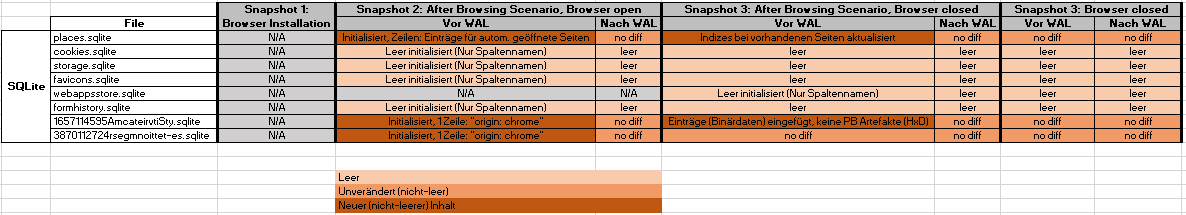
\includegraphics{bilder/firefox-sqlite-table.png}}}
	\label{chart:final-criteria}  
	\caption{Comparison of found PB artifacts between RAM Dumps}
\end{figure}
Nach Browser-Installation (Snapshot 1) existierte noch keine der SQLite-Dateien.

Nach dem Browsing Szenario (Snapshot 2) wurde festgestellt, dass alle SQLite-Datenbanken 
initialisiert wurden, außer \texttt{webappsstore.sqlite}. Dabei wurden in \texttt{places.sqlite} die automatisch im normalen Modus geöffnete Datenschutzhinweise Seite eingetragen. 
In restlichen Datenbanken wurden leer initialisiert, nur die Spaltennamen wurden eingetragen.
Der Inhalt aller erstellten Datenbanken blieb nach Durchführung von PRAGMA WAL Checkpoints unverändert.

Nach Schließen des Browsers (Snapshot 3) wurden in \texttt{places.sqlite} die Indizes bei eingetragenen Seiten aktualisiert. Die SQLite-Datenbank \texttt{1657114595AmcateirvtiSty.sqlite} erhielt ein binäres Datenobjekt als Eintrag. Bei der Untersuchung mit HxD konnten keine Artefakte gefunden werden. Weiterhin wurde \texttt{webappsstore.sqlite} leer initialisiert. Die restlichen Daten blieben im Vergleich mit Snapshot 2 unverändert. Ebenfalls veränderte sich nicht der Inhalt nach Durchführung von PRAGMA WAL Checkpoints.

Nach herunterfahren der VM (Snapshot 4) gab es keine Änderungen in den SQLite Datenbanken, auch nach Durchführung der PRAGMA WAL Checkpoints.
	
Somit wurden in den SQLite Datenbanken von Firefox keine zurückverfolgbaren PB Artefakte im privaten Modus hinterlassen.


Mithilfe des Process Monitors wurde festgestellt, dass sowohl während des Browsing Szenarios (Logfile 1) als auch danach (Logfile 2) Inhalte in Dateien geschrieben wurden. Wie zusammenfassend in Abbildung X (TODO!) dargestellt, wurde mit Ausnahme der Datareporting Dateien gab es in Logfile 1 stets mehr oder genauso viele Schreiboperationen wie in Logfile 2.
Keine Schreiboperation hinterließ jedoch Private Browsing Artefakte.
\begin{figure}[h!]
	\centerline{\resizebox{\linewidth}{!}{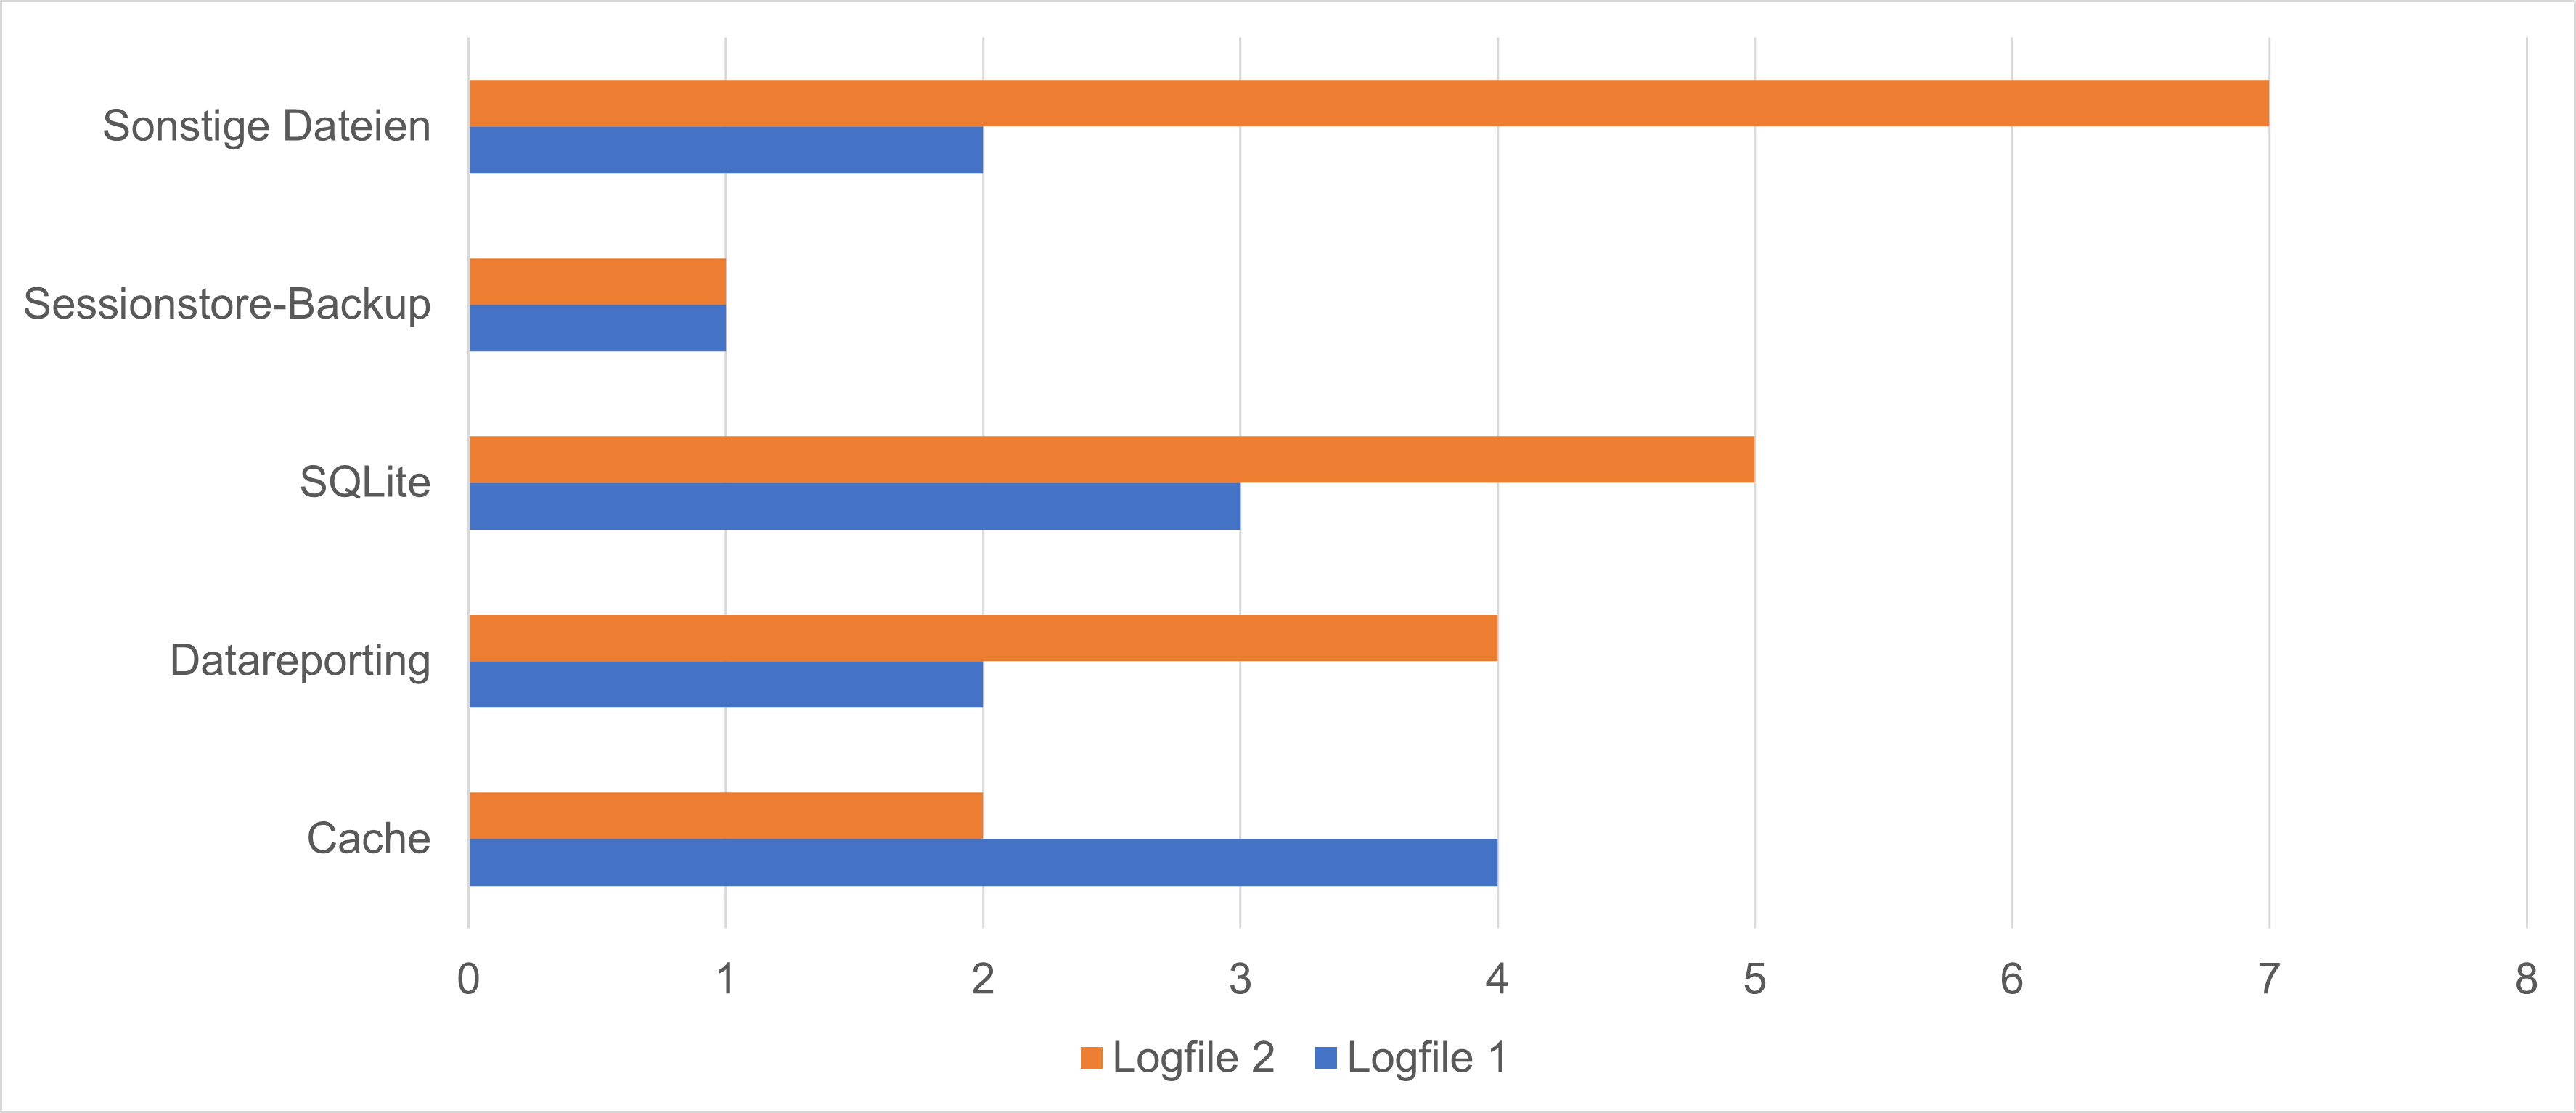
\includegraphics{bilder/bar-chart-logfile1vs2-test.png}}}
	\label{chart:final-criteria}  
	\caption{Comparison of found PB artifacts between RAM Dumps}
\end{figure}


%Literatur:
%	o no traces were found in “common locations” \cite{Montasari.2015}
%		>  “places.sqlite”, “webappsstore. sqlite”, “sessionstore.bak”, “search.json” and “nssckbi.dll”
%	o	Safebrowsing: Alle Dateien in /safebrowsing-updating/ nicht relevant. Dort nur .vlpset und .sbstore Dateien. Speichern 256-Bit Hash von URLs, die auf SafeSearch Blacklist stehen 
%	o	Cache-Dateien: drei Caches: startupCache, jumpListCache (beide enthalten Binärdateien ohne Browsing Artefakte) und cache2 (können mit MozillaCacheView untersucht werden, enthalten keine Browsing Artefakte)
%	o	SQLite Datenbanken: Sqlite Dateien erst ohne WAL Dateien untersuchen, Danach mit sqlite3 Konsole: WAL in Datenbank schreiben mit: PRAGMA wal\_checkpoint; places.sqlite besonders relevant, da dort Browser in public Modus Browsing URLs verwaltet (Am besten hier vergleich mit Public Browsing machen)	
%		> \cite{Fayyad.2021} for Mozilla Firefox, 7 database files were recovered: cookies.sqlite-shm, places.sqlite-shm, prefs.js etc.
%		> \cite{Muir.2019} The two SQLite databases used by Firefox to track cookies and history (cookies.sqlite und places.sqlite) were both recoverable from the file system after deletion	
%		Ergebnisse stehen im Gegensatz zu \cite{Hedberg.2013} :
%			o	Chrome und Firefox: Einträge in places.sqlite + history.sqlite DB gefunden während PB! (Noch aktuell??)
%		Sonderfall: SQlite DB-Crash \cite{Hedberg.2013}
%			> WAL Files/Journal Files bei Crash gefunden -> Kann genutzt werden um zu beweisen, dass privater Browser genutzt wurde
%			> Daher: WAL Rollback mit sqlite3	
%	o	Jsonlz4 \& balkz4: Enthalten komprimierte Firefox-Sessions, jsonlz4 Dateien können mit Tool "entkomprimiert" werden: https://www.jeffersonscher.com/ffu/scrounger.html

\subsection*{Uncommon Locations}

Nachfolgend werden die Analyseergebnisse der Firefox Uncommon Locations beschrieben.
Wie in Kapitel X erläutert, wird im Gegensatz zu Common Locations die Suchrichtung umgekehrt und es werden alle gesammelten Daten nach einem spezifischen PB Artefakt durchsucht.
Somit benötigt ein Forensiker kein Wissen über das Browserverhalten. Stattdessen wird sich auf die Vollständigkeit der Funktionen von Forensik-Tools verlassen. Im Rahmen dieses Versuchs werden die Tools Autopsy und Volatility verwendet.

\subsubsection*{Analyse mit Autopsy}

Bei den Common Locations in Kapitel X wird Autopsy nur zur Dateiextraktion genutzt. Im Falle der Uncommon Locations dient Autopsy als forensisches Werkzeug zur Datenanalyse.

Eine Autopsy Stichwortsuche gemäß Methodik in Kapitel X (TODO!) lieferte in allen Snapshots keine Treffer. Es wurde zusätzlich das \texttt{\$Carved} Verzeichnis durchsucht, in dem Autopsy alle wiederhergestellten Dateien speichert.

Anschließend wurden die automatisch von Autopsy kategorisierten Dateien untersucht. Gemäß Methodik in Kapitel X wurden dazu die Dateien der Kategorien "Web Bookmarks", "Web Cookies", "Web History" sowie "Web Categories" analysiert.
Beim Vergleich der Festplattenabbilder wurde festgestellt, dass ein Snapshot stets die kategoriesierten Dateien des vorherigen Snapshots enthielt. Es sind innerhalb einer Kategorie nur neue Dateien dazugekommen. Somit enthält Snapshot 4 in jeder Kategorie alle Dateien der vorherigen Snapshots.

\paragraph*{Web Bookmarks}

Bereits vor Durchführung des Browsing Szenarios enthielt Firefox im ersten Snapshot die Bing Startseite als gespeichertes Leesezeichen. In den restlichen Snapshots 2 -- 4 blieb diese Kategorie unverändert.

\begin{figure}[h!]
	\centerline{\resizebox{\linewidth}{!}{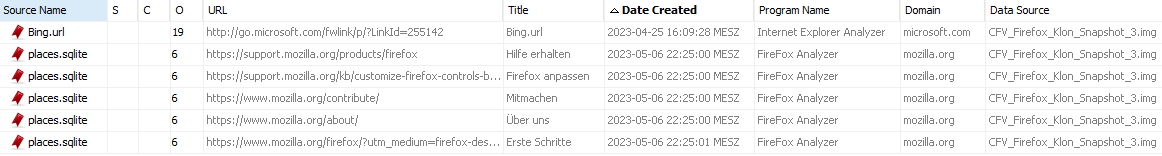
\includegraphics{bilder/cfv_firefox_autopsy_web_bookmarks.png}}}
	\label{chart:final-criteria}  
	\caption{Autopsy Web Bookmarks}
\end{figure}

\paragraph*{Web Cookies}
Auch diese Kategorie enthält bereits vor Beginn des Browsing Szenarios zehn Cookie-Einträge in der Datei \texttt{WebCacheV01.dat}. Dabei handelt es sich um eine Datenbank des Microsoft Edge Browsers zur Speicherung von Nutzerdaten. Diese Datei verhält sich ähnlich wie die in diesem Versuch relevanten SQLite-Dateien. Die Datei enhält. Bei den Einträgen handelt es sich um Cookies für Bing und die Outlook Webseite, obwohl diese Seiten nie in Microsoft Edge geöffnet wurden. In den Snapshots 2 -- 4 kamen keine weiteren Einträge in dieser Kategorie hinzu.
\begin{figure}[h!]
	\centerline{\resizebox{\linewidth}{!}{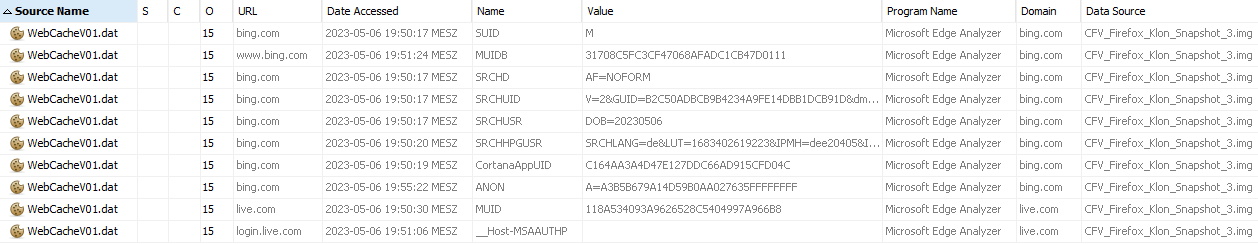
\includegraphics{bilder/cfv_firefox_autopsy_web_cookies.png}}}
	\label{chart:final-criteria}  
	\caption{Autopsy Web Cookies}
\end{figure}

\paragraph*{Web History}
Diese Kategorie listet alle Dateien mit gespeichertem Suchverlauf auf. Vor Beginn des Browsing Szenarios (Snapshot 1) enthält die Kategorie ebenfalls zwei Einträge zur Outlook Webseite in der Datei \texttt{WebCacheV01.dat}. Nach Durchführung des Browsing Szenarios (Snapshot 2) wurde ein Eintrag in der \texttt{places.sqlite} Datenbank hinzugefügt. Dabei handelt es sich um die automatisch im normalen Browsingmodus geöffnete Firefox-Standardseite über Datenschutzhinweise. Dies deckt sich mit den Beobachtungen der Common Locations in Kapitel X. Darüber hinaus enthält dieser Snapshot für die Datei \texttt{WebCacheV01.dat} den Eintrag \texttt{file:///Z:/Logfile\_1}. Dabei handelt es sich um das Process Monitor Logfile, das gemäß Methodik in Kapitel X (TODO!) über den gemeinsamen VM-Ordner zum Analyse-Rechner transportiert wurde. Ergänzt wird das in Snapshot 3 durch den Eintrag \texttt{file:///Z:/Logfile\_2}, dem zweiten Process Monitor Logfile. In Snapshot 4 werden in dieser Katgeorie keine neuen Dateien erfasst.
\begin{figure}[h!]
	\centerline{\resizebox{\linewidth}{!}{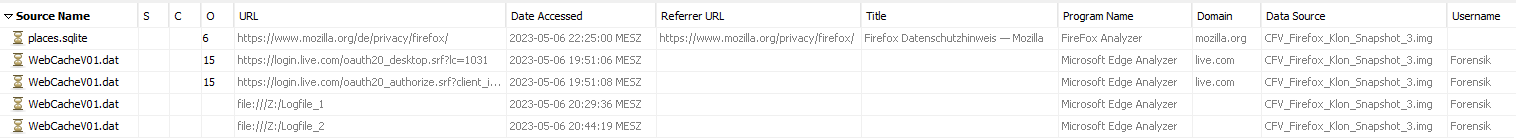
\includegraphics{bilder/cfv_firefox_autopsy_web_history.png}}}
	\label{chart:final-criteria}  
	\caption{Autopsy Web History}
\end{figure}

\paragraph*{Web Categories}
Diese Kategorie klassifiziert im Speicherabbild gefundene Browsing Artefakte nach Inhalt.
Vor Beginn des Browsing Szenarios (Snapshot 1) werden hier bereits zwei Einträge aufgelistet. Der Eintrag \texttt{bing.com} wird als "Suchmaschine" klassifiziert und \texttt{live.com} als "Web-Email".
Wie oben erwähnt, wurden beide Seiten nie aufgerufen. Es gab keine zusätzlichen Einträge in dieser Kategorie in den Snapshots 2 bis 4.
\begin{figure}[h!]
	\centerline{\resizebox{\linewidth}{!}{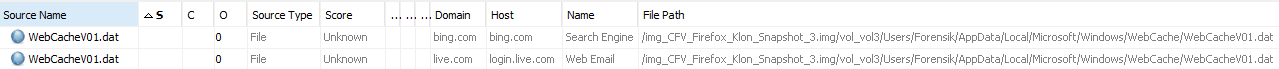
\includegraphics{bilder/cfv_firefox_autopsy_web_categories.png}}}
	\label{chart:final-criteria}  
	\caption{Autopsy Web Categories}
\end{figure}
		

Somit wurden in allen Kategorien ausschließlich Browsing Artefakte des Edge Browsers in der Datei \texttt{WebCacheV01.dat} gefunden, sowie ein Eintrag in der Firefox SQLite Datenbank \texttt{places.sqlite}. Die eingetragene Firefox-Standardseite deckt sich mit den Ergebnissen der Common Locations in Tabelle X. Die aufgelisteten Einträge in der Datei \texttt{WebCacheV01.dat} sind nicht auf Schritte des Browsing Szenarios zurückzuführen. Die Einträge sind bereits im ersten Snapshot enthalten, obwohl vor Beginn des Browsing Szenarios keine Browseraktivitäten durchgeführt wurden. Weiterhin enthölt diese Datei Einträge über die Process Monitor Logfiles, welche über einen gemeinsamen VM-Ordner zum Rechner transportiert wurde, auf dem die virtuelle Maschine läuft.
In keiner der Kategorien konnten private Browsing Artefakte identifiziert werden.

%Literatur:
%	o	Autopsy Keywortsuche: 
%		>	In alles Snapshots ergebnislos (keine Keyword-Hits
%		-->	In Literatur: Autoren fanden Ergebnisse in pagefile.sys 
%			> Autopsy: websites and some of the keywords found in hidden file called “pagefile.sys” \cite{Mahlous.2020}
%			o \cite{Montasari.2015} traces were found in: 
%				> However, on investigating the “pagefile.sys”, some entries were discovered
%				> Using the “data carving” technique, profile picture was recovered
%			o \cite{Said.2011} 
%				> Examining pagefile.sys showed some positive hits 			
%		--> Evtl. hier zeigen, was gefunden werden kann, wenn RAM reduziert
%		--> Aber auf Problem hinweisen, dass gefundener String in pagefile nicht direkt Browser zugeordnet werden kann
%		> \cite{Gabet.2018}	Firefox only produced three recoverable artefacts as reported by both tools (FTK, Autopsy) --> Artefakte werden nicht genannt!
%		> \cite{Muir.2019} Autopsy Keyword Suche nach Suchbegriffen: unallocated space
%		> Autopsy Carving Module (\$Carved): \cite{Muir.2019}
%			•	When searching for the string ’clot’ from the browsing protocol, six .dll, .edb and .reg files were discovered in unallocated space.
%			•	Further searching of unallocated space uncovered references to the Tor installation directory and the obfs4 bridging IP addresses
%			•	browsing data found in NTUSER.DAT was also replicated in unallocated space.
%	o	Autopsy PlugIns:
%		>	*** TODO: Hier Liste mit PlugIns ***

\subsubsection*{Analyse mit Volatility}
Nachdem die Firefox Festplattenabbilder als Uncommon Location mit Autopsy untersucht wurden, werden nachfolgend die Analyseergebnisse des RAMs als Uncommon Location beschrieben. 
Dazu wurde eine Stringsuche im gesamten RAM nach PB Artefakten durchgeführt.
Wie in Kapitel X ausführlich beschrieben muss ein gefundener String eindeutig einem Browser zugeordnet werden können. 
Deshalb wurde dazu das Volatility PlugIn "Yarascan" verwendet, ein Werkzeug um nach bestimmten Mustern im RAM zu suchen. Dazu wurden die in Tabelle X aufgeführten Yara-Regeln verwendet.
Wie in Kapitel Methodik (TODO!) beschrieben, wird davon ausgehend das PlugIn "pslist" verwendet, um den Prozessnamen anhand PID zu identifizieren.
Die Ergebnisse dieser Stringsuche sind nachfolgend nach Kategorie geordnet.

\paragraph*{Yararule HTML}
In keinem der Firefox RAM Dumps wurden HTML Fragemente der besuchten Seiten gefunden. Somit wird diese Yara-Regel nicht weiter betrachtet.

\paragraph*{Yararule Keyword}
Wie in Abbildung X (TODO!) gezeigt, wurden alle Suchbegriffe "pfaffenhofen", "nanoradar", "mooserliesl" sowie "mallofamerica" identifiziert im zwiten RAM Dump, nach dem Browsing Szenario mit geöffnetem Browser, identifiziert. Die Artefakte befinden sich ausschließlich im zweiten RAM Dump. Die Suchbegriffe wurden größtenteils in den Speicherbereichen von Firefox-Prozessen gefunden. Nur in zwölf Fällen wurden Suchbegriffe in anderen Prozessen identifiziert. Am häufigsten wurde der Suchbegriff "pfaffenhofen" mit 1301 gefundenen Artefakten im zweiten Firefox RAM Dump gefunden. Dies ist vermutlich auf den Google Maps Kartenbereich zurückzuführen, einen visuellen Ausschnitt der Karte, welcher bei der Google-Suche erscheint und Informationen über die geografische Lage, Straßen, Sehenswürdigkeiten und andere relevante Orte in der gesuchten Stadt zeigt. In den RAM Dumps 1 und 3 konnten Artefakte zu den Suchbegriffen identifiziert werden.
\begin{figure}[h!]
	\centerline{\resizebox{\linewidth}{!}{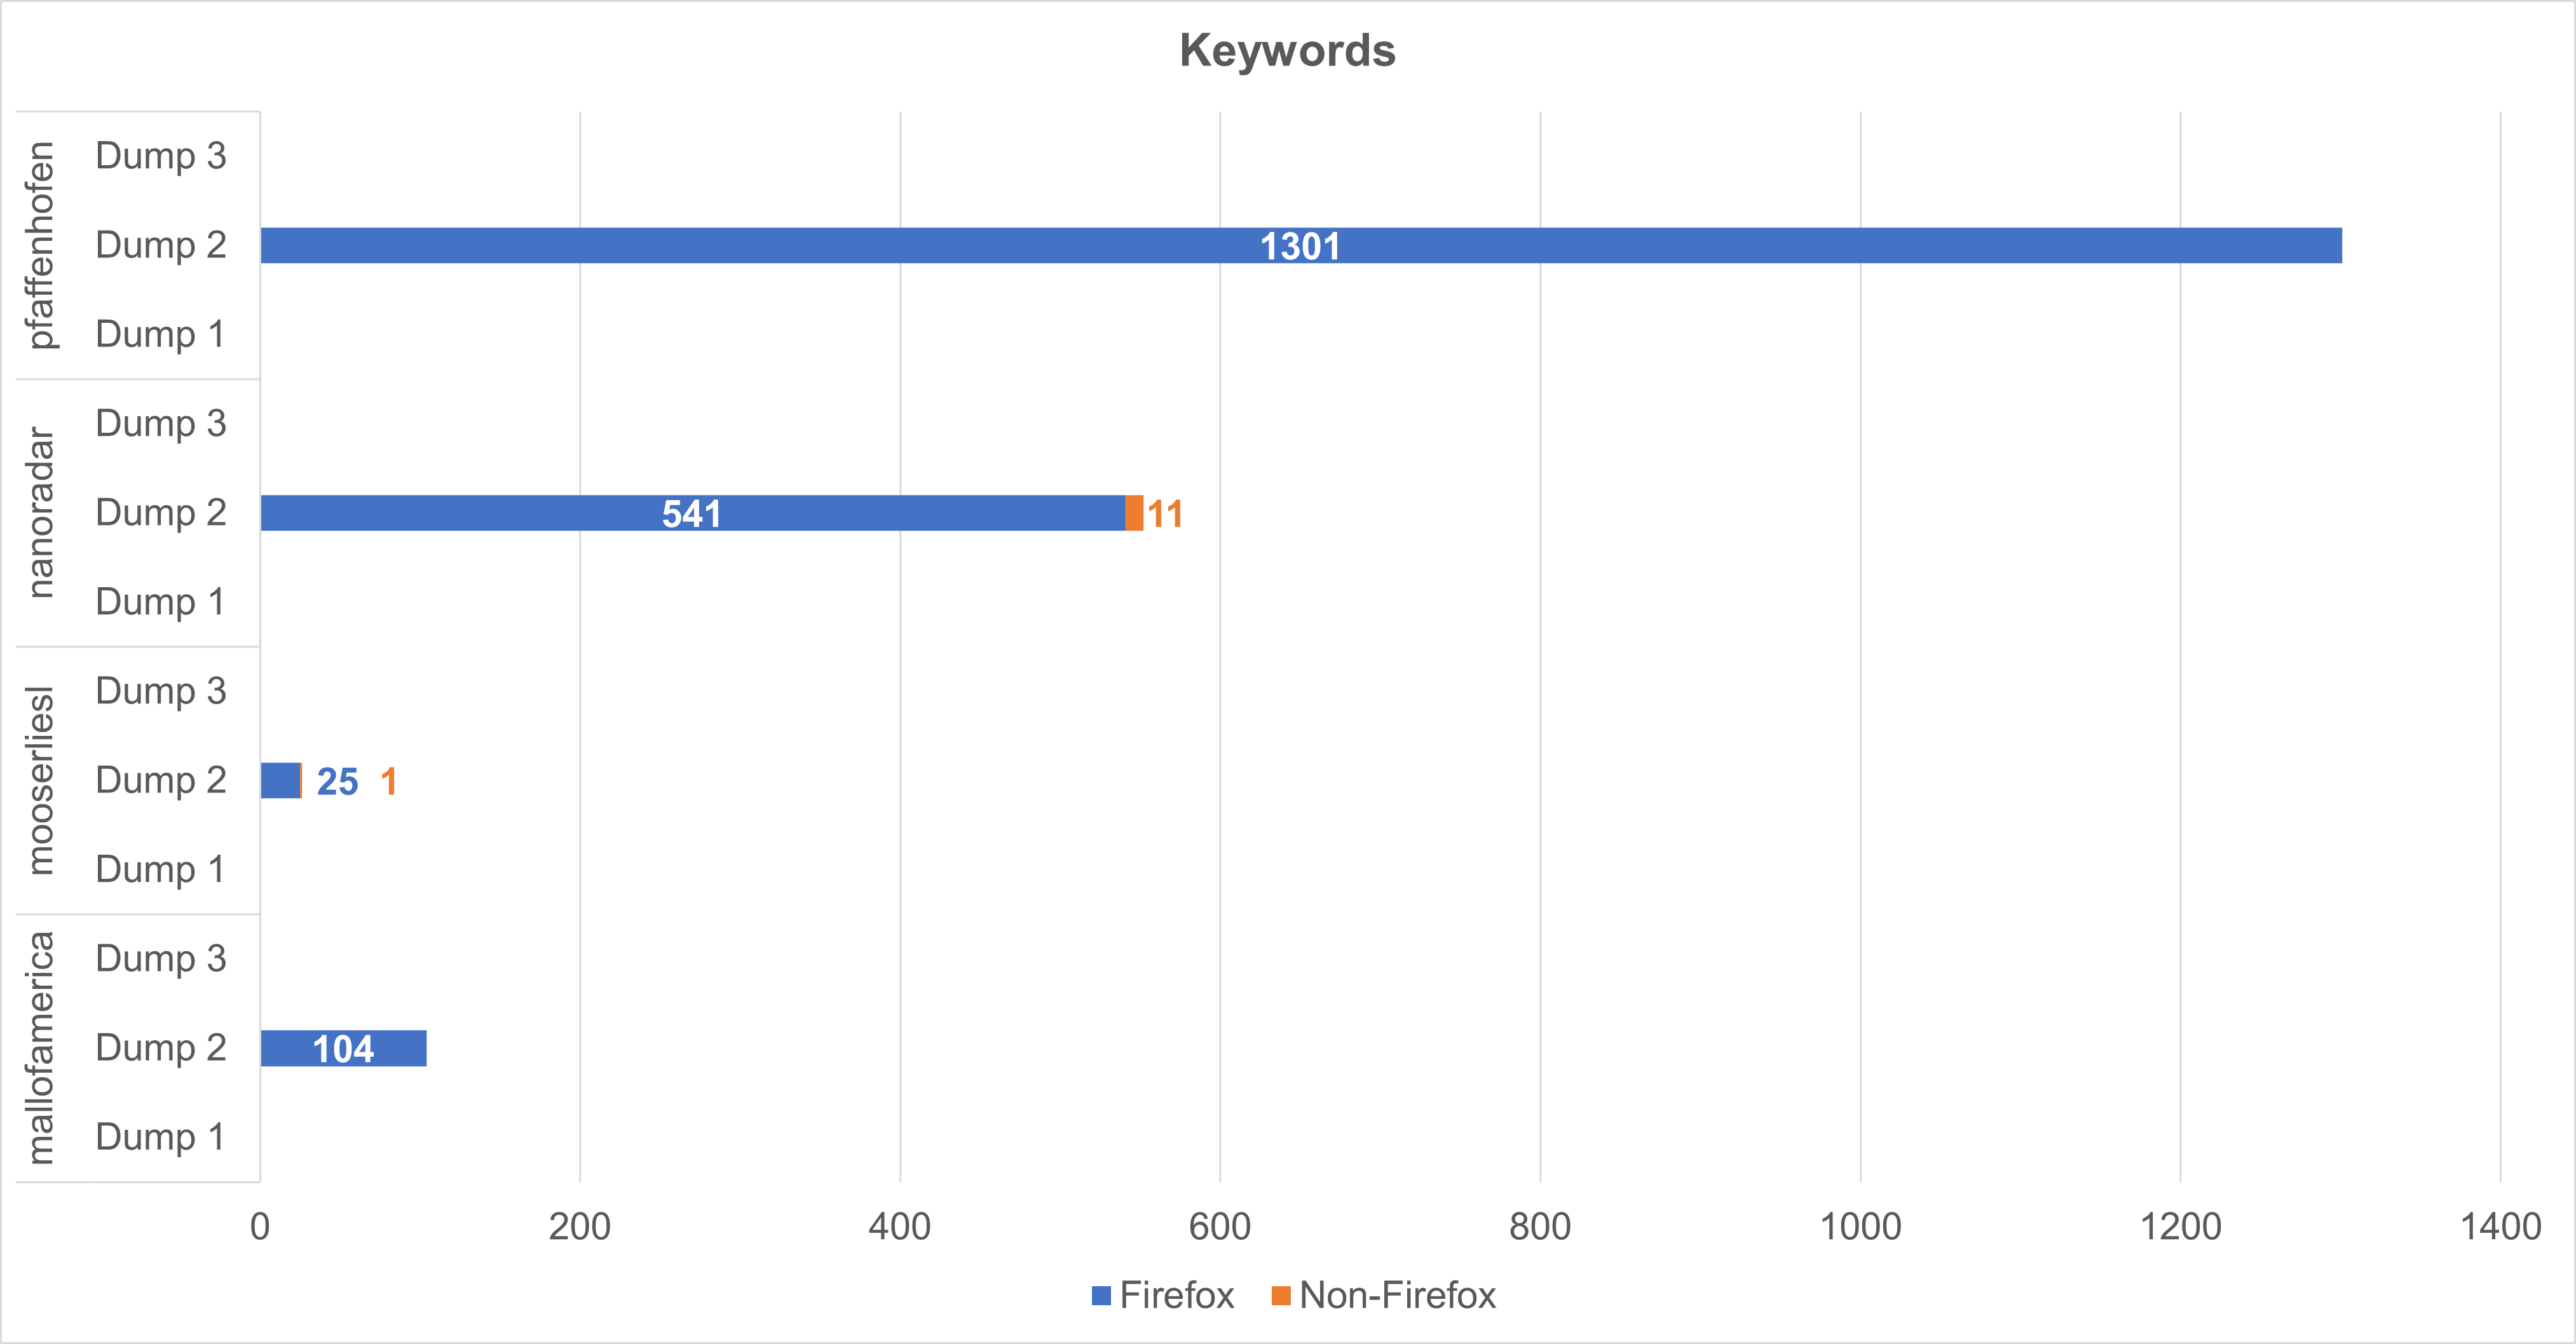
\includegraphics{bilder/volatility/firefox/keywords.png}}}
	\label{chart:final-criteria}  
	\caption{Keywords}
\end{figure}

\paragraph*{Yararule URL}
\begin{figure}[h!]
	\centerline{\resizebox{\linewidth}{!}{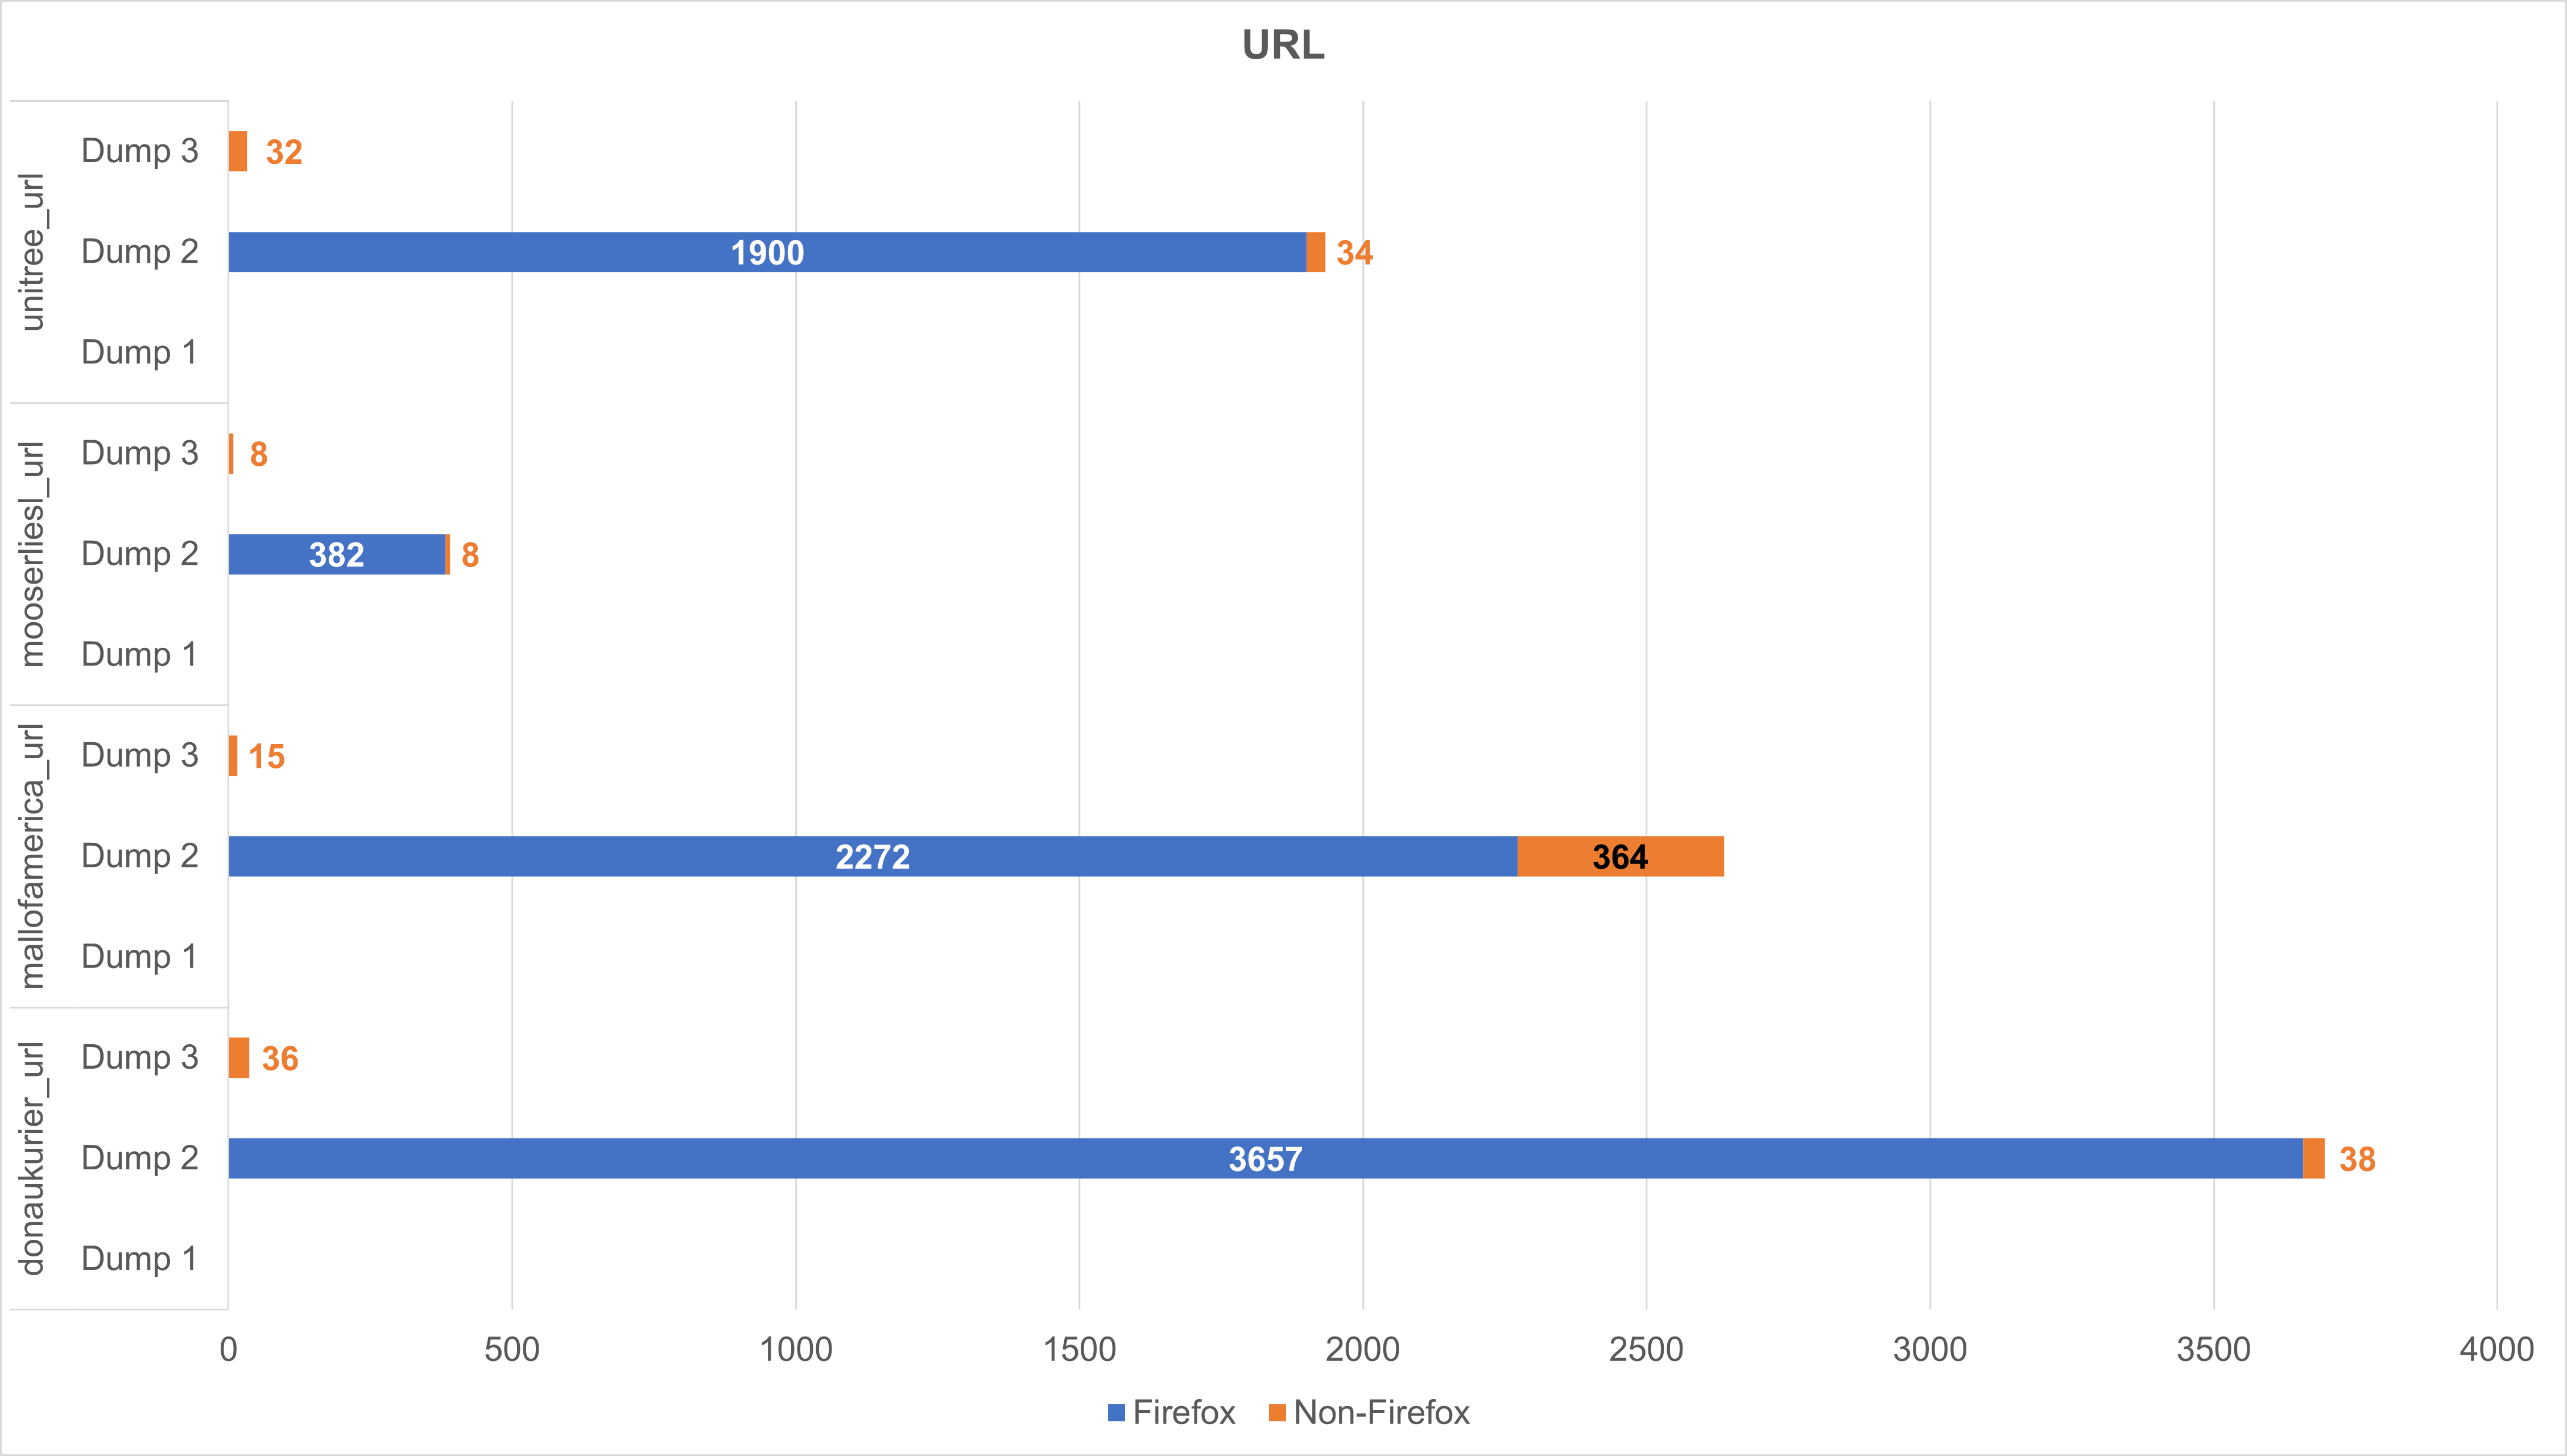
\includegraphics{bilder/volatility/firefox/url.png}}}
	\label{chart:final-criteria}  
	\caption{URL}
\end{figure}
Es konnten in den Arbeitsspeicherabbildern alle besuchten URLs unitree.com, mooserliesl.de, mallofamerica.com sowie donaukurier.de identifiziert werden.
Dabei wurden die meisten Artefakte nach dem Browsing Szenario mit geöffnetem Browser (RAM Dump 2) gefunden. Alle besuchten URLs wurden in diesem Dump sowohl in Firefox als auch anderen Prozessen gefunden, wobei die meisten Artefakte in Firefox Prozessen zu finden sind. Dabei wurde "mooserliesl.de" mit insgesamt 390 Artefakten am wenigsten gefunden, "donaukurier.de" mit über 3600 Artefakten am häufigsten.

Bemerkenswert ist, dass URL Artefakte gefunden wurden, nachdem der Browser geschlossen wurde (RAM Dump 3). Dabei wurde kein URL Artefakte in einem Firefox Prozess gefunden.
Anhand der PID $2252$ wurde festgestellt, dass sich alle URL Artefakte des dritten RAM Dumps in einem "svchost.exe" Prozess mit der gleichen PID befinden. Unter dem "Service Host" Prozess laufen gruppierte Windows-Dienste, um Ressourcen zu sparen und die Systemleistung zu verbessern.
Volatility bietet das Plugin "svcscan" an, mit dem alle laufenden Dienste ausgegeben werden können.
Bei Anwendung auf den dritten RAM Dump wurde jedoch zu keinem Dienst eine PID angegeben, wordurch der Dienst mit den URL Artefakten nicht im RAM identifiziert werden konnte. 
% https://learn.microsoft.com/de-de/windows/application-management/svchost-service-refactoring
Stattdessen wurde der dritte Snapshot aufgetaut, um im laufenden Windowsbetrieb den Dienst mithilfe des Process Explorers zu identifizieren.
Wie in Abbildung X (TODO!) gezeigt, wurde anhand der PID $2252$ der Dienst "DNSCache" ermittelt.
\begin{figure}[h!]
	\centerline{\resizebox{\linewidth}{!}{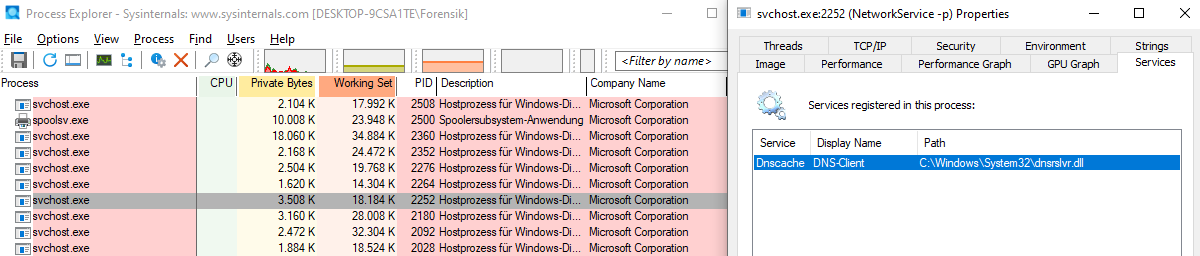
\includegraphics{bilder/firefox-dnscache.png}}}
	\label{chart:final-criteria}  
	\caption{URL}
\end{figure}
Der DNSCache-Dienst unter Windows ist ein Teil des Betriebssystems, der für die Übersetzung von Domainnamen in IP-Adressen verantwortlich ist. Der DNSCache-Dienst speichert DNS-Anfragen und Antworten temporär, umd wiederholte DNS-Anfragen zu beschleunigen.
% https://learn.microsoft.com/en-us/answers/questions/47441/how-to-disable-windows-10-dns-cache-services
Nach Löschen des DNSCaches mit dem Kommandozeilenbefehl \texttt{ipconfig /flushdns}, dem Schließen aller Process Monitor Instanzen sowie Beenden des DNSCaches Services wurde erneut ein RAM-Dump durchgeführt. Dort wurden keine URL Artefakte mehr gefunden.

\paragraph*{Yararule Mail}
\begin{figure}[h!]
	\centerline{\resizebox{\linewidth}{!}{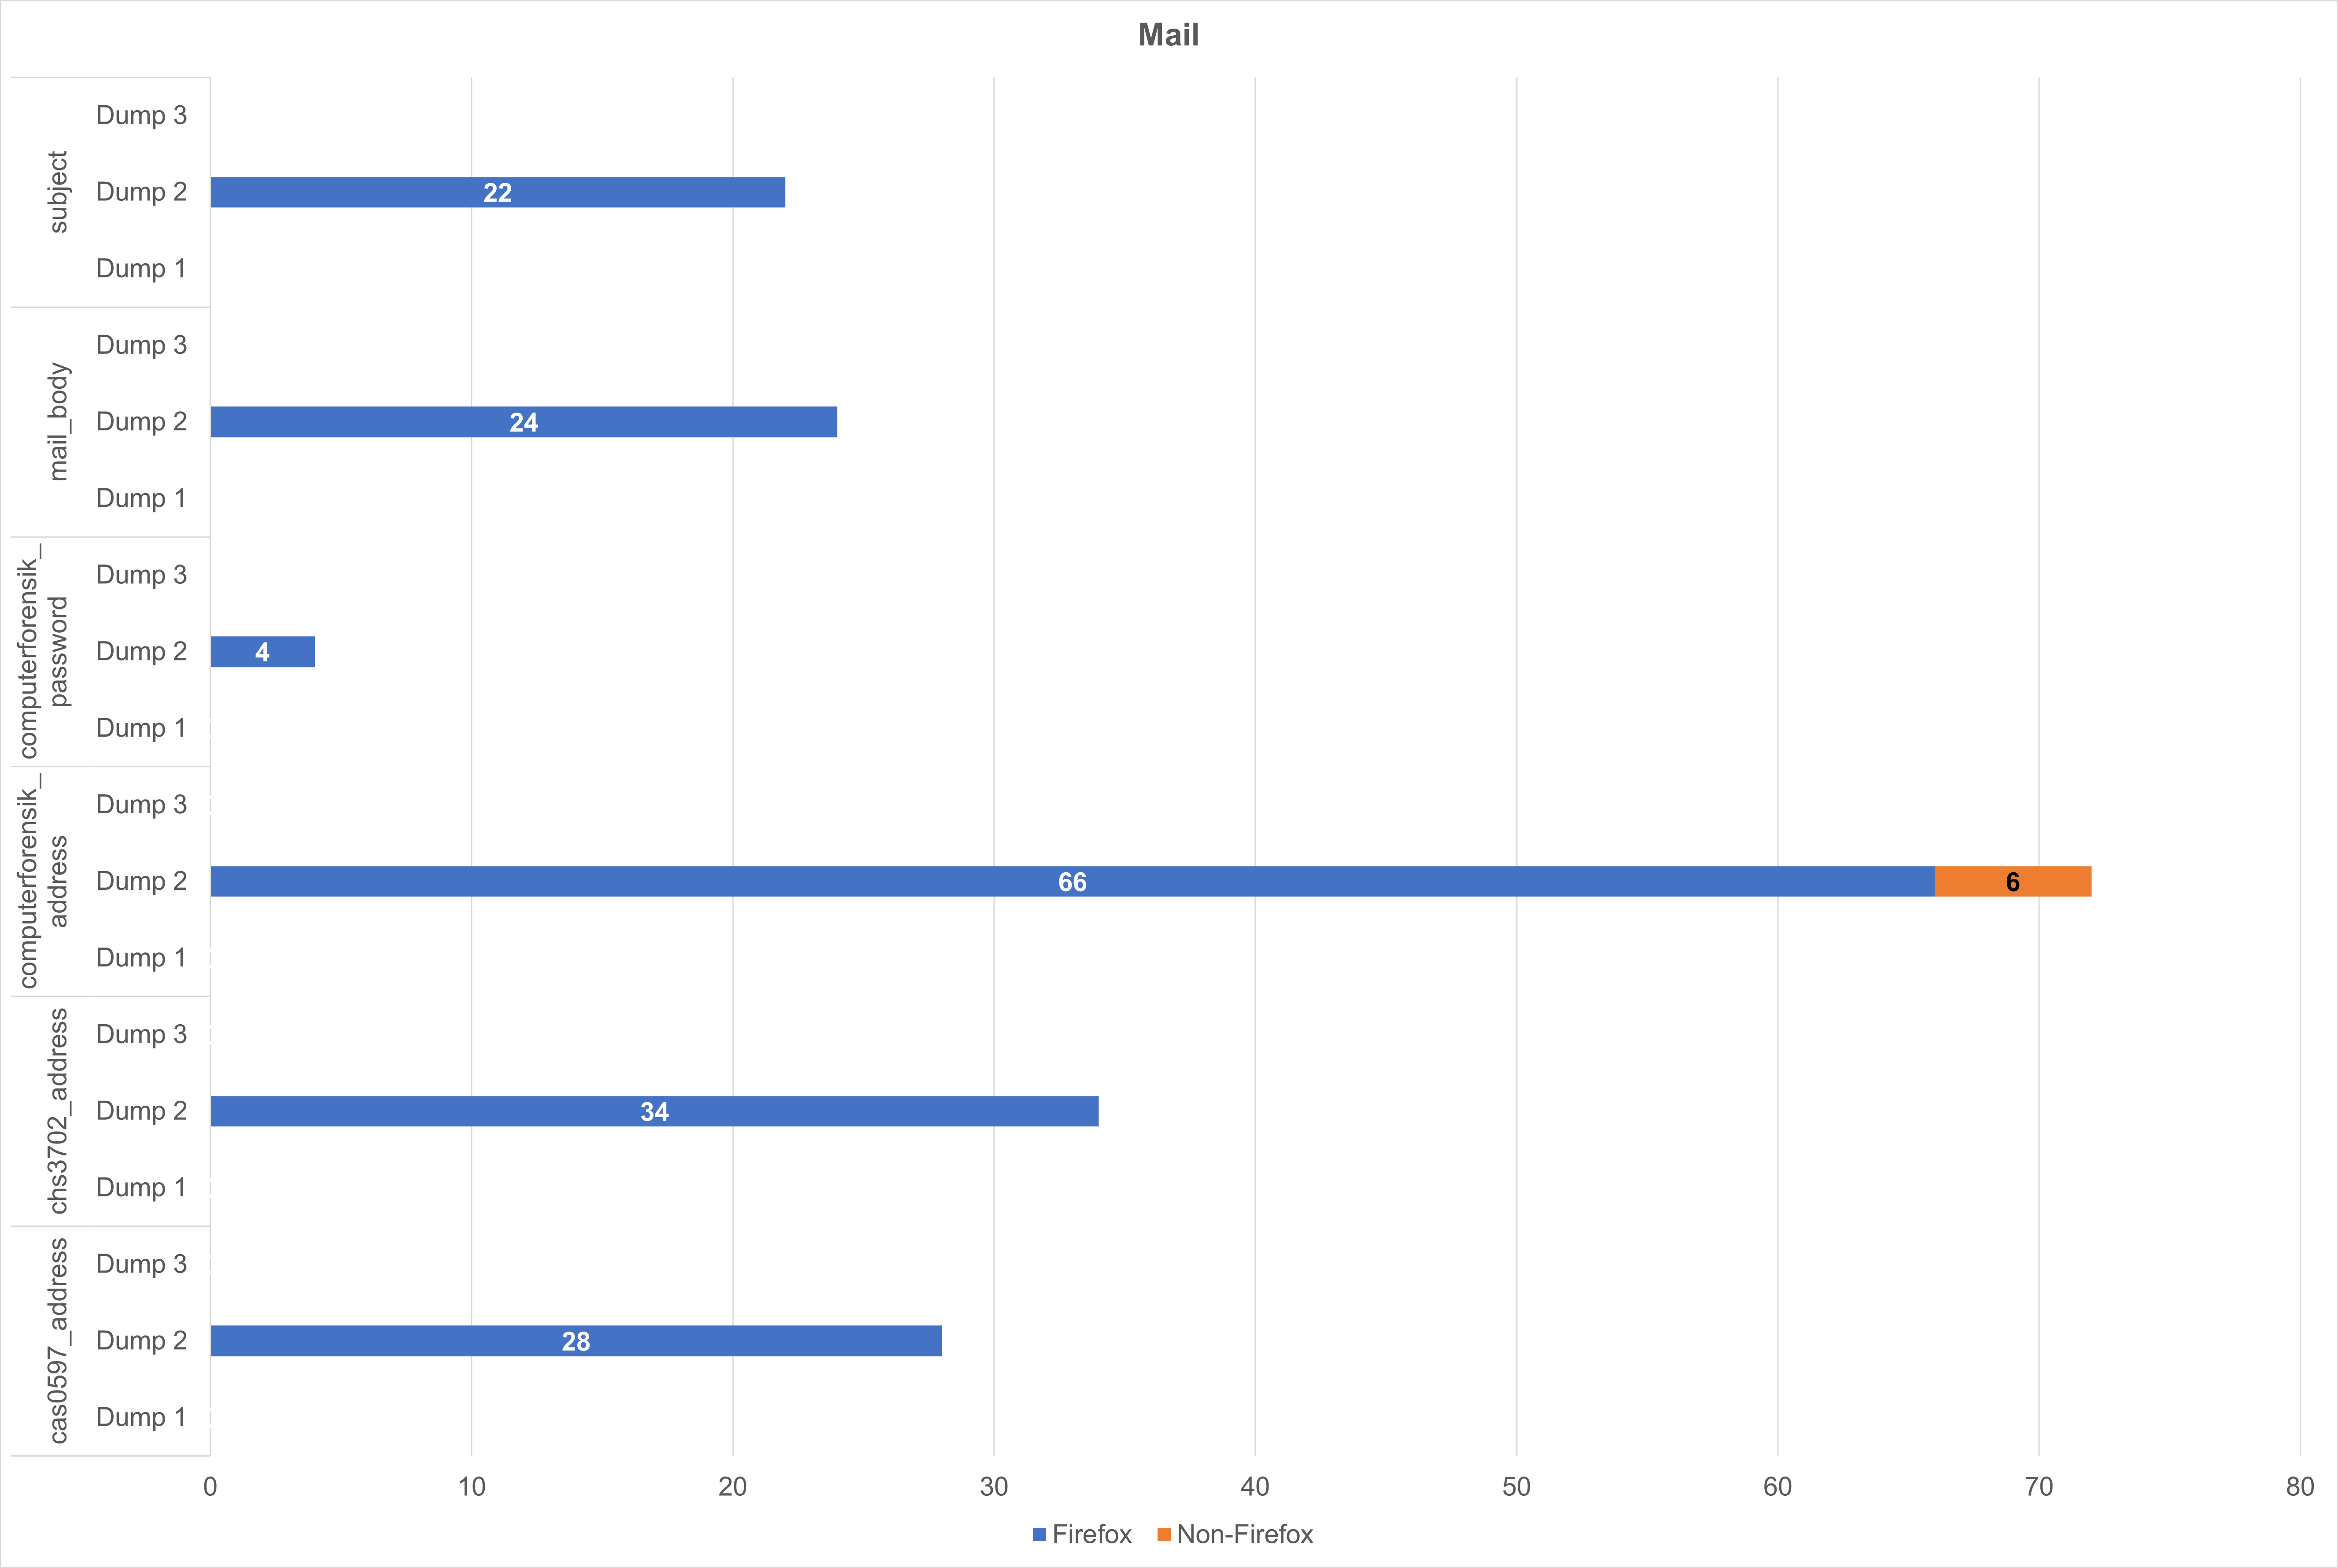
\includegraphics{bilder/volatility/firefox/mail.png}}}
	\label{chart:final-criteria}  
	\caption{Mail}
\end{figure}
Es konnten alle E-Mail Artefakte des Browsing Szenarios gefunden werden.
Die Artefakte befinden sich ausschließlich im zweiten Firefox RAM Dump, nach dem Browsing Szenario mit geöffnetem Browser.
Unter den gefundenen Artefakten befindet sich mit zwölf Vorkommen am häufigsten die Absenderadresse "computerforensikvl@gmail.com". Dieses Artefakt wurde als einziges Mail-Artefakt in anderen Prozesses außer Firefox gefunden.

Bemerkenswert ist, dass das Passwort des Google-Accounts, mit dem die E-Mails verschickt wurden, vier mal als Klartext im RAM gefunden wurden. Das Passwort wurde in je zwei Firefox Prozessen mit den PIDs 7420 und 8424 zwei mal gefunden. Tabelle X zeigt die virtuellen Speicheradressen der Artefakte aus der Yarascan Ausgabe.
\begin{table}[]
\resizebox{\linewidth}{!}{
\begin{tabular}{|c|c|c|ll}
\cline{1-3}
\textbf{Virtuelle Speicheradresse} & \textbf{PID} & \textbf{Byte-Offset in extrahierter Speicherseite} &  &  \\ \cline{1-3}
0xb9ce29180c8                      & 7420         & 0x11dd40c8                                         &  &  \\ \cline{1-3}
0x2859f4ffd4e0                     & 7420         & 0x12e234e0                                         &  &  \\ \cline{1-3}
0x24083b41858                      & 8424         & 0x583858                                           &  &  \\ \cline{1-3}
0x240840e5b08                      & 8424         & 0x96bb08                                           &  &  \\ \cline{1-3}
\end{tabular}
}
\end{table}

Zu diesen Artefakten wurde gemäß Methodik in Kapitel X der String Kontext -- die Zeichen vor und nach dem gefundenen Artefakt im Speicherbereich -- ermittelt. Dazu wurde gemäß Methodik in Kapitel X mithilfe des Volatility memmap-Plugins die Abbildung der virtuellen Speicheradressen auf den Byte-Offset in der extrahierten Speicherseite des Prozesses ermittelt. 
\begin{figure}[h!]
	\centerline{\resizebox{0.7\linewidth}{!}{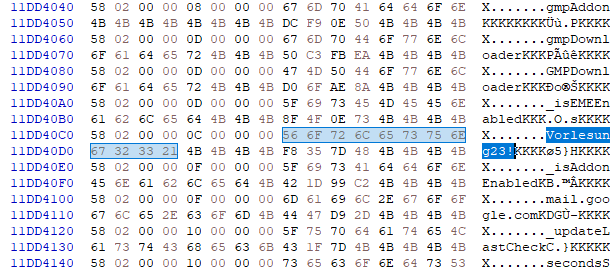
\includegraphics{bilder/volatility/firefox/password_0xb9ce29180c8_7420.png}}}
	\label{chart:final-criteria}  
	\caption{Password in memory page of PID 7420 at Byte-Offset 0x11dd40c8}
\end{figure}
Wie in Abbildung X gezeigt, sind in der Speicherseite des Prozesses mit PID $7420$ konnte vor und nach dem gefundenen Passwort am Byte-Offset $0xb9ce29180c8$ neben der Gmail-Url "mail.google.com" Code-Fragmente der "Gecko-Engine" zu finden. Dieser Teil des Firefox Browsers ist für das Rendering von Webinhalten verantwortlich, einschließlich HTML, CSS, JavaScript und anderen Medienformaten wie Bildern, Audio und Video.
% https://wiki.mozilla.org/GeckoMediaPlugins
\begin{figure}[h!]
	\centerline{\resizebox{0.7\linewidth}{!}{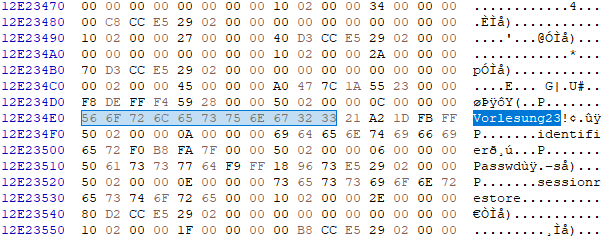
\includegraphics{bilder/volatility/firefox/password_0x2859f4ffd4e0_7420.png}}}
	\label{chart:final-criteria}  
	\caption{Password in memory page of PID 7420 at Byte-Offset 0x12e234e0}
\end{figure}
In der gleichen Datei konnte nach dem gefundenen Passwort am Byte-Offset $0x24083b41858$ die Strings "Passwd" sowie "sessionrestore" (siehe Common Location "Sessionstore" in Kapitel X) identifiziert werden. 
Wie in den Abbildungen X und Y (TODO!) gezeigt, können in den Byte-Offsets der gefundenen Passwörter in der Speicherseite der PID 8424 konnten kein Kontext ermittelt werden. Im Gegensatz zur Speicherseite der PID 7420 wird das Passwort dort mit 2 Bytes pro Zeichen enkodiert. Das eine Unicode-Zeichenenkodierung vermuten.
\begin{figure}[h!]
	\centerline{\resizebox{0.7\linewidth}{!}{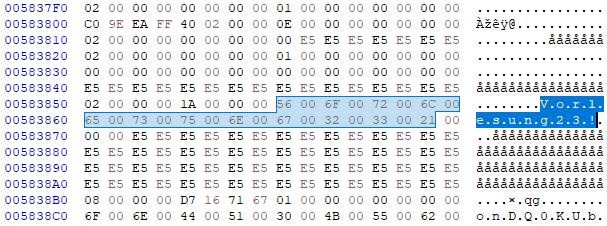
\includegraphics{bilder/volatility/firefox/password_0x24083b41858_8424.png}}}
	\label{chart:final-criteria}  
	\caption{Password in memory page of PID 8424 at Byte-Offset 0x583858}
\end{figure}
\begin{figure}[h!]
\centerline{\resizebox{0.7\linewidth}{!}{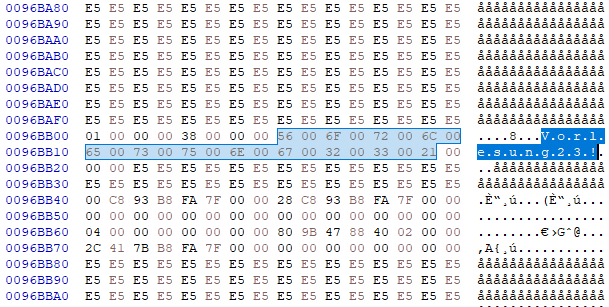
\includegraphics{bilder/volatility/firefox/password_0x240840e5b08_8424.png}}}
\label{chart:final-criteria}  
\caption{Password in memory page of PID 8424 at Byte-Offset 0x96bb08}
\end{figure}
				
\paragraph*{Yararule Image}
Das im Browsing Szenario geöffnete Donaukurier Logo wurde ausschließlich im zweiten RAM Dump in drei mal in Firefox Prozessen gefunden.
\begin{figure}[h!]
	\centerline{\resizebox{\linewidth}{!}{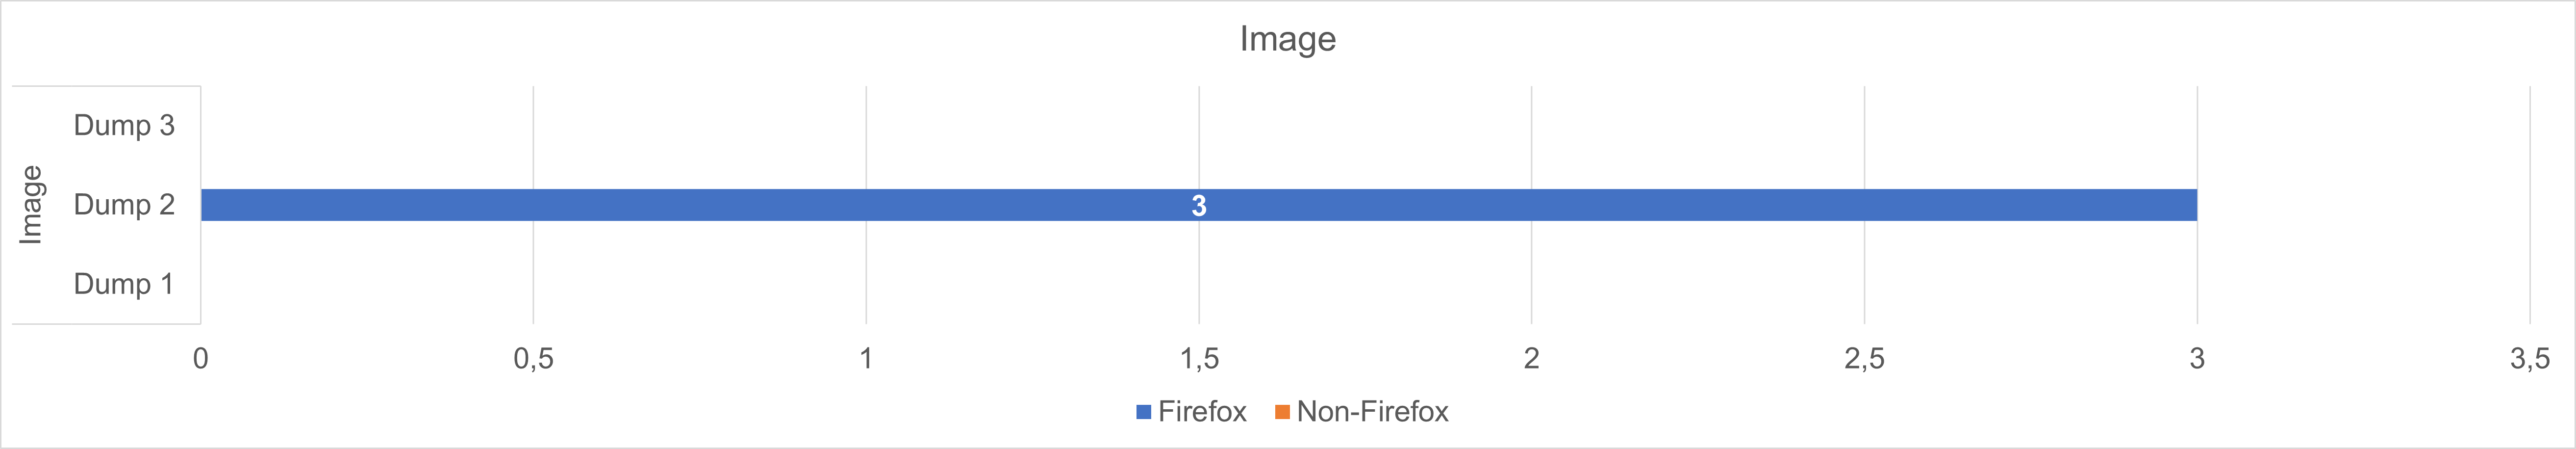
\includegraphics{bilder/volatility/firefox/image.png}}}
	\label{chart:final-criteria}  
	\caption{Image}
\end{figure}

Wie in Abbildung X zusammenfassend gezeigt wurden vor dem Browsing Szenario, keine private Browsing Artefakte im ersten RAM Dump gefunden.
Nach dem Browsing Szenario mit geöffnetem Browser konnten die meisten Artefakte identifiziert werden. Dabei wurden am häufigsten URL Artefakte in Firefox Prozessen gefunden. Zudem konnte hier das E-Mail Passwort im Klartext lokalisiert werden.
Nach Schließen des Browsers konnten im dritten Snapshots URLs im DNSCache Windows Service gefunden werden. Nach leeren des Caches und Beenden des DNSCache Services konnten wurden keine Artefakte gefunden.
\begin{figure}[h!]
	\centerline{\resizebox{\linewidth}{!}{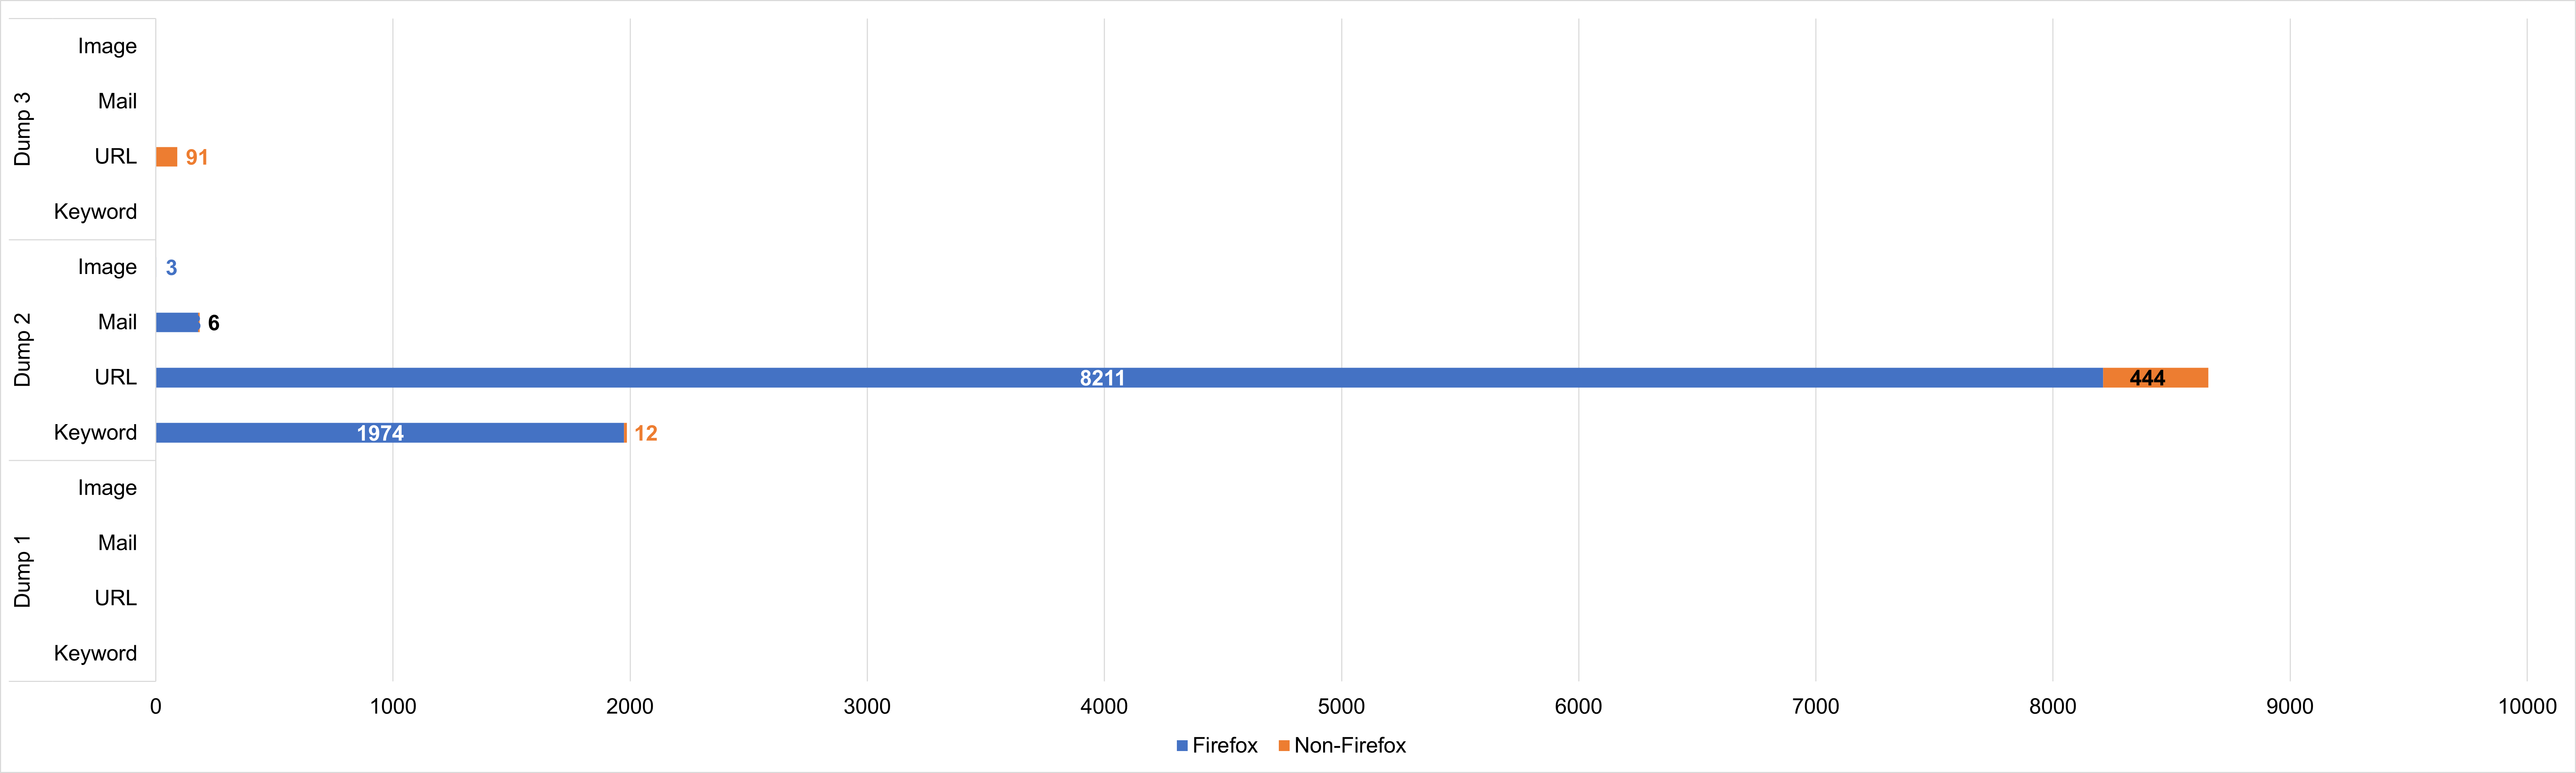
\includegraphics{bilder/volatility/firefox/summary.png}}}
	\label{chart:final-criteria}  
	\caption{Summary}
\end{figure}


\subsection*{Registry}

Die Analyse der Registry zählt gemäß Methodik in Kapitel X sowohl zu den Common als auch Uncommon Locations 

\subsubsection*{Process Monitor SetValue Operations}

Als Teil der Common Locations werden für Firefox alle Registry "SetValue" Schreiboperationen der beiden Process Monitor Logfiles untersucht.

In beiden Logfiles wurden zwei Kategorien von Registry Keys geschrieben: "PreXULSkeletonUISettings" und "Business Activity Monitoring". In Abbildung X ist der Anteil der Schreiboperationen je Kategorie für beide Logfiles gezeigt.
\begin{figure}[h!]
	\centerline{\resizebox{\linewidth}{!}{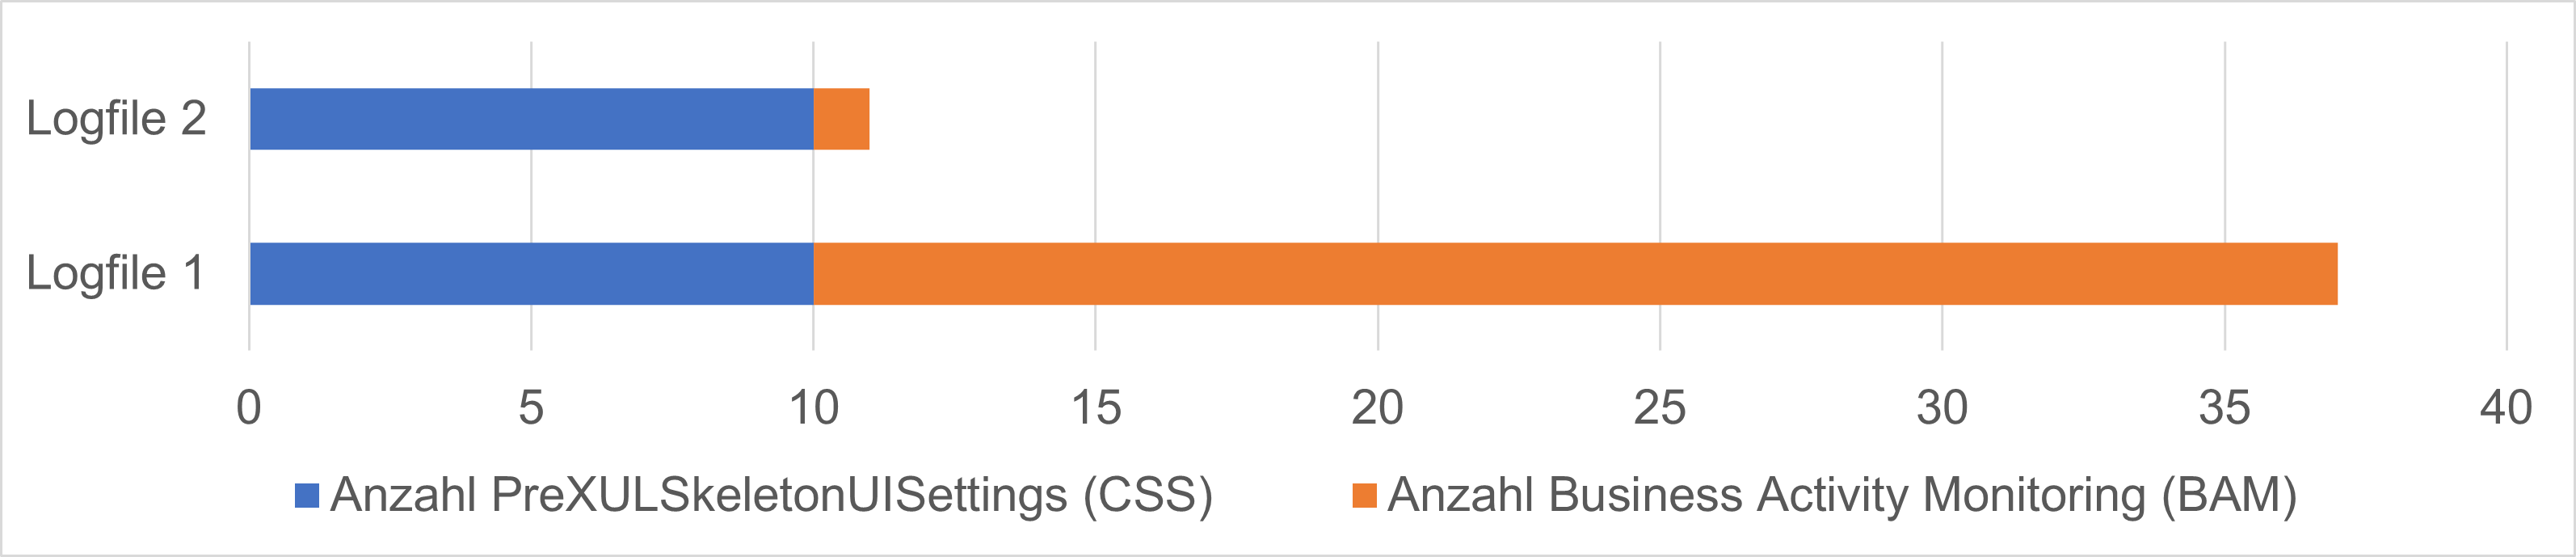
\includegraphics{bilder/firefox-registry-stacked-bar-chart.png}}}
	\label{chart:final-criteria}  
	\caption{Comparison of found PB artifacts between RAM Dumps}
\end{figure}

\paragraph*{PreXULSkeletonUISettings}
%https://itigic.com/skeleton-ui-new-firefox-interface-to-start-up-much-faster/#google_vignette
Der "PreXULSkeletonUISettings" Registry Key enthält Einstellungen für die Benutzeroberfläche (UI) des Firefox-Browsers, insbesondere für das sogenannte "Skeleton UI, eine vereinfachte Benutzeroberfläche, die während des Ladens des Browsers angezeigt wird, bevor die vollständige Benutzeroberfläche geladen ist. 
PreXULSkeletonUISettings Registry Keys haben das Format \texttt{HKCU$\backslash$SOFTWARE$\backslash$Mozilla$\backslash$Firefox$\backslash$PreXULSkeletonUISettings$\backslash$<Absoluter Firefox Installationspfad>$\backslash$firefox.exe|<Skeleton UI Setting>}.
Somit enthält der Key den absoluten Installationspfad von Firefox gefolgt von einer Skeleton UI Einstellung. Nachfolgend sind alle möglichen UI Einstellungen aufgelistet, gefolgt vom Datentyp des Keys.
\begin{itemize}
	\item ScreenX (DWORD)
	\item ScreenY (DWORD)
	\item Width (DWORD)
	\item Height (DWORD)
	\item Maximized (DWORD)
	\item Flags (DWORD)
	\item CssToDevPixelScaling (REG\_BINARY)
	\item UrlbarCSSSpan (REG\_BINARY)
	\item SearchbarCSSSpan (REG\_BINARY)
	\item SpringsCSSSpan (REG\_BINARY)
\end{itemize}
Somit enthalten die Keys nur Daten zur Formatierung und Struktur der grafischen Oberfläche. Es wurden keine PB Artefakte geschrieben

\paragraph*{Business Activity Monitoring}
"Business Activity Monitoring", kurz BAM ist eine weitgehend undokumentierte Windows Funktion, die im Hintergrund ausgeführte Programme steuert.
Der Registry Key hat das Format \texttt{HKLM$\backslash$System$\backslash$CurrentControlSet$\backslash$Services$\backslash$bam$\backslash$State$\backslash$UserSettings$\backslash$<SID>$\backslash$Device$\backslash$HarddiskVolume2$\backslash$<Absoluter Firefox Installationspfad>$\backslash$firefox.exe} und den Datentyp REG\_BINARY.
Jeder Schlüssel wird durch die Sicherheits-ID (SID) des Benutzers identifiziert.
Ein BAM Registry Key schreibt für alle ausgeführten Programme --- hier Firefox --- den Zeitstempel der letzten Ausführung.
PB Artefakte sind dabei nicht enthalten.
% https://learn.microsoft.com/de-de/biztalk/core/business-activity-monitoring-bam
% https://notes.qazeer.io/dfir/windows/_artefacts_overview 

\subsubsection*{Stringsuche in Registry Hives}
Gemäß Methodik in Kapitel X wird die Firefox Registry als Uncommon Location behandelt, indem über alle auf der Festplatte vorhandenen Registry Datenbanken, den Registry-Hives, eine Stringsuche durchgeführt wird, ohne die Struktur der Hives zu beachten. 
Dazu wurden sowohl die System-Hives als auch die User-Hives aus Tabelle X (TODO!) aus jedem Snapshot extrahiert und mithilfe des Registry Explorers nach PB Artefakten durchsucht.
Dabei wurde in keinem Snapshot in keinem Hive ein PB Artefakt gefunden.

%Literatur:
%	>	Auf Autor verweisen: angeblich in Shellactivities Ergebnisse. --> Nicht mehr vorhanden in aktueller Version (Verweis auf E-Mail)
%	>	Process Monitor/Regshot zeigen keine relevanten Key-Änderungen
%	> \cite{Muir.2019}: Autopsy Keyword Suche nach Suchbegriffen: Ergebnisse in \%SystemRoot\%Minidump NTUSER.DAT, ntuser.dat.LOG1 (a log of changes to NTUSER.DAT)
%	> Zentral: shellactivites Key:	NTUSER.DAT --> “shellactivities” key \cite{Muir.2019}
%	> \cite{Rochmadi.2017} Detection of registry changes helps to determine what the appropriate plugin is used to search for digital evidence using volatility memory forensic:
%	- RegQueryValue:	HKCU/Software/Microsoft/Windows/CurrentVersion/InternetSettings/Connections/DefaultConnectionSettings
%	- RegCloseValue: 	HKCU/Software/Microsoft/Windows/CurrentVersion/InternetSettings/Connections
%	- IRP\_MJ\_READ: C:/pagefile.sys


*** TODO: Zusammenfassung Firefox ***


\newpage


% ######################################################################
% ######################################################################
% ######################################################################
% ######################################################################


\section{Tor}

\subsection*{White-Box Analyse/Common Locations}

Schreiboperationen mit Process Monitor verfolgen:

Im Anhang: Tabelle mit allen geschriebenen Dateien (markiert, wenn nicht mehr wiederherstellbar + markiert, wenn Datei "verändert" (siehe oben: temp, WAL))

Aux-Dateien, welche nicht mehr vorhanden waren, aber dafür "richtige" Dateien:

Ergebnis: Tabelle mit wiederherstellbaren Dateien: Logfile 1 vs. Logfile 2 + Tool mit dem Datei untersucht wurde
- Dateien, die in beiden Logfiles nicht wiederherstellbar 
\begin{figure}[h!]
	\resizebox{\linewidth}{!}{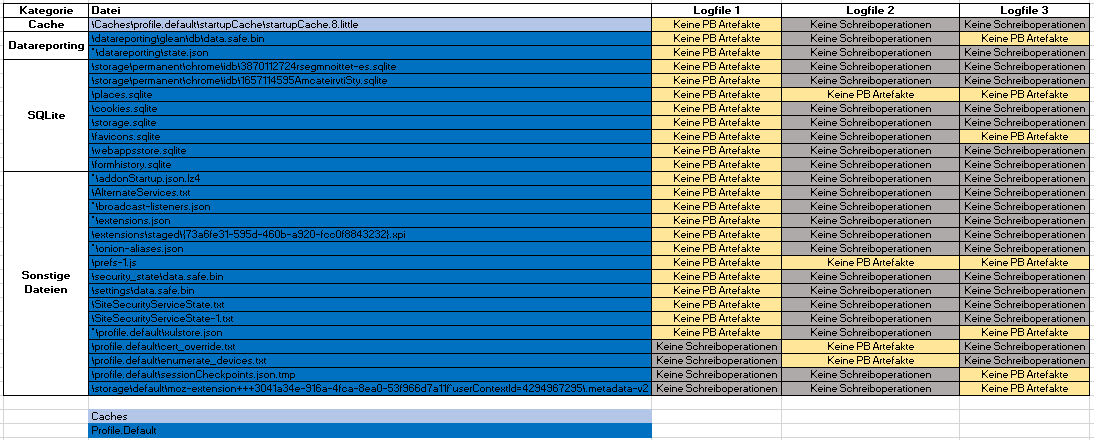
\includegraphics{bilder/tor-tabelle-logfile1vlogfile2vlogfile3-reduced.png}}
%	\label{...}
	\caption{Tabelle mit wiederherstellbaren Dateien: Logfile 1 vs. Logfile 2}
\end{figure}

Allgemein: Tor hat nur einen "Common Pfad"
-	% C:\Users\Forensik\Desktop\Tor Browser\Browser\TorBrowser\Data\Browser\
- Dateien tauchen in zwei unterschiedlichen Ordnern auf:
	- % C:\Users\Forensik\Desktop\Tor Browser\Browser\TorBrowser\Data\Browser\Caches\profile.default\ (Caches)
	- % C:\Users\Forensik\Desktop\Tor Browser\Browser\TorBrowser\Data\Browser\profile.default\ (Profile.Default)

- Alle Schreibopertationen von Prozess "firefox.exe" durchgeführt, nicht "tor.exe" 

=> Keine der Dateien enthält PB Artefakte, trotzdem nachfolgende genauere Betrachtung der wichtigsten Dateien im Zusammenhang des Tor Browsers

Kategorien der Logs:
- Cache: 
	> % \Caches\profile.default\startupCache\startupCache.8.little (Caches Folder)
	Zweck:
		"Die Datei "startupCache.8.little" ist eine interne Datei, die von Firefox und dem Tor Browser erstellt wird, um den Startvorgang des Browsers zu beschleunigen. Sie enthält im Wesentlichen eine Zwischenspeicherung von Daten, die beim Starten des Browsers benötigt werden.

		Diese Datei enthält Informationen über bereits geladene Browser-Komponenten wie JavaScript-Code, CSS-Dateien, Bilder und andere Ressourcen. Indem der Browser diese Informationen zwischenspeichert, kann er sie beim erneuten Starten des Browsers wiederverwenden, anstatt sie erneut herunterladen und verarbeiten zu müssen. Dadurch wird die Startzeit des Browsers verkürzt und die allgemeine Leistung verbessert." %https://wiki.mozilla.org/StartupCache
	Analyse:
		- Tool: HxD
		- kein PB Artefakte

- datareporting:
	> % *\datareporting\state.json 
	Zweck: 
		"Die Datei "state.json" im Ordner "/datareporting" enthält Informationen über den Zustand und die Konfiguration des Firefox- oder Tor Browsers. Diese Datei kann Daten über die Verwendung des Browsers, wie z.B. installierte Add-Ons, zuletzt besuchte Websites, Browser-Einstellungen und andere Informationen enthalten. Sie wird verwendet, um dem Browser bei Bedarf den Zustand und die Einstellungen wiederherzustellen."
		% https://github.com/mozilla/firefox-data-store-docs/blob/master/README.md
	Analyse:
		- Tool Notepad++ mit JSON Plugin
		- keine PB Artefakte

- Sonstige Dateien:
	> % \AlternateServices.txt
		Zweck:
			"enthält onion URLs,
			HTTP Alternative Services is a mechanism that allows servers to tell clients that the service they are accessing is available at another network location or over another protocol.
			This mapping can be stored in a file in the profile folder. This allows websites that do not support HTTPS to communicate in a secure way via port 443 (Opportunistic Encryption)."
			% https://support.mozilla.org/en-US/questions/1310302
	> % \extensions\staged\{73a6fe31-595d-460b-a920-fcc0f8843232}.xpi
		Zweck:
			"Ist "NoScript" Extension. Wenn in Firefox geöffnet, kann installiert werden"
		=> TODO: Screenshot, wenn in Firefox per "drag-and-drop" gezogen
	> % *\onion-aliases.json
		Zweck:
			Enthält SecureDrop Adressen: z.B. sueddeutsche.securedrop.tor.onion (z.B. %https://www.sueddeutsche.de/projekte/kontakt/#securedrop)
	> % \security_state\data.safe.bin
		Zweck: The file containing the updated security data % (https://bbs.archlinux.org/viewtopic.php?pid=1952286#p1952286)
	> % \SiteSecurityServiceState.txt
		Entielt früher private Browsing Artefakte (https://gitlab.torproject.org/tpo/applications/tor-browser/-/issues/18589), jetzt aber keine private Browsing Artefakte
	=> Keine der Dateien enthält PB Artefakte
				
- SQLite: 
	Aus Process Monitor Logfiles erkennbar: Tor verwaltet und beschreibt die exakt gleichen SQLite Datenbanken wie Firefox.

	Hier ebenfalls gesondert betrachtet: Fokus auf die Entwicklung von Dateiinhalt in allen Snapshots (1, 2, 3-1, 3 und 4) betrachtet
	
	Ergebnisse:
		\begin{figure}[h!]
			\centerline{\resizebox{\linewidth}{!}{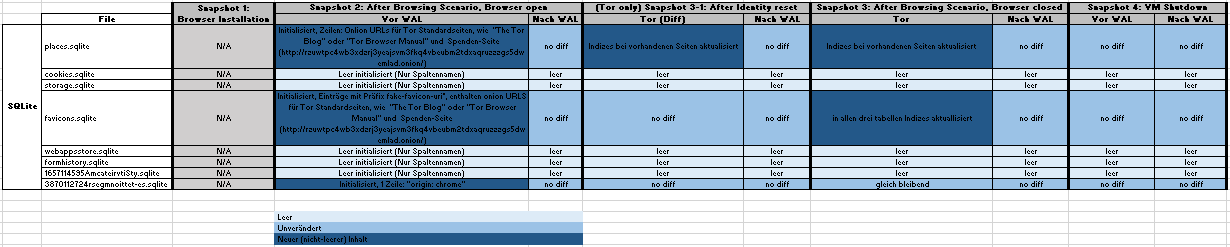
\includegraphics{bilder/tor-sqlite-table.png}}}
			\label{chart:final-criteria}  
			\caption{Comparison of found PB artifacts between RAM Dumps}
		\end{figure}
		> Nach Browser-Installation noch keine SQLite-Datei angelegt (Snapshot 1)
		> Während Browsing Szenario alle DBs Initialisiert, außer "webappsstore.sqlite" (Snapshot 2)
			- Dabei wurden in places.sqlite automatisch .onion URLs geschreiben, die zu Tor Standardseiten führen, wie "The Tor Blog" oder "Tor Browser Manual" bzw. die Tor Spenden-Seite, obwohl keine dieser Seiten aufgerufen wurde
				TODO: Screenshot von URLs?
			- in Favicons.sqlite wurden die exakt gleichen Enträge geschrieben, mit dem Präfix "Fake-favicon-uri". Ein tatsächliches Icon wurde nicht in die DB geschrieben
			- remote settings Datenbank enthielt den gleichen Eintrag wie es bereits bei Firefox der Fall war. Keine PB Artefakte
			- Restliche Dateien ohne Inhalt, nur Spaltennamen
			- Nach WAL Checkpoints bleiben Dateien unverändert
		> Nach Zurücksetzen der Browser-Identität (Snapshot 3-1)
			- in places.sqlite: Indizes bei eingetragenen Seiten aktualisiert
			- restliche Dateien unverändert
		> Nach Schließen des Browsers (Snapshot 3)
			- in places.sqlite sowie favicons.sqlite: Indizes bei eingetragenen Seiten aktualisiert
			- restliche Dateien unverändert
			- nach WAL Checkpoints bleiben Dateien unverändert
		> Nach herunterfahren der VM (Snapshot 4)
			- Alle Dateien unverändert, auch nach WAL Checkpoint
	
- Zusammenfassung: in keiner Datei PB Artefakte


Quantitativ: (Diagramme)		
	> Balkendiagramm: Für jede Logfilekategorie: Anzahl Schreiboperationen Logfile 1 vs Logfile 2
	\begin{figure}[h!]
		\centerline{\resizebox{\linewidth}{!}{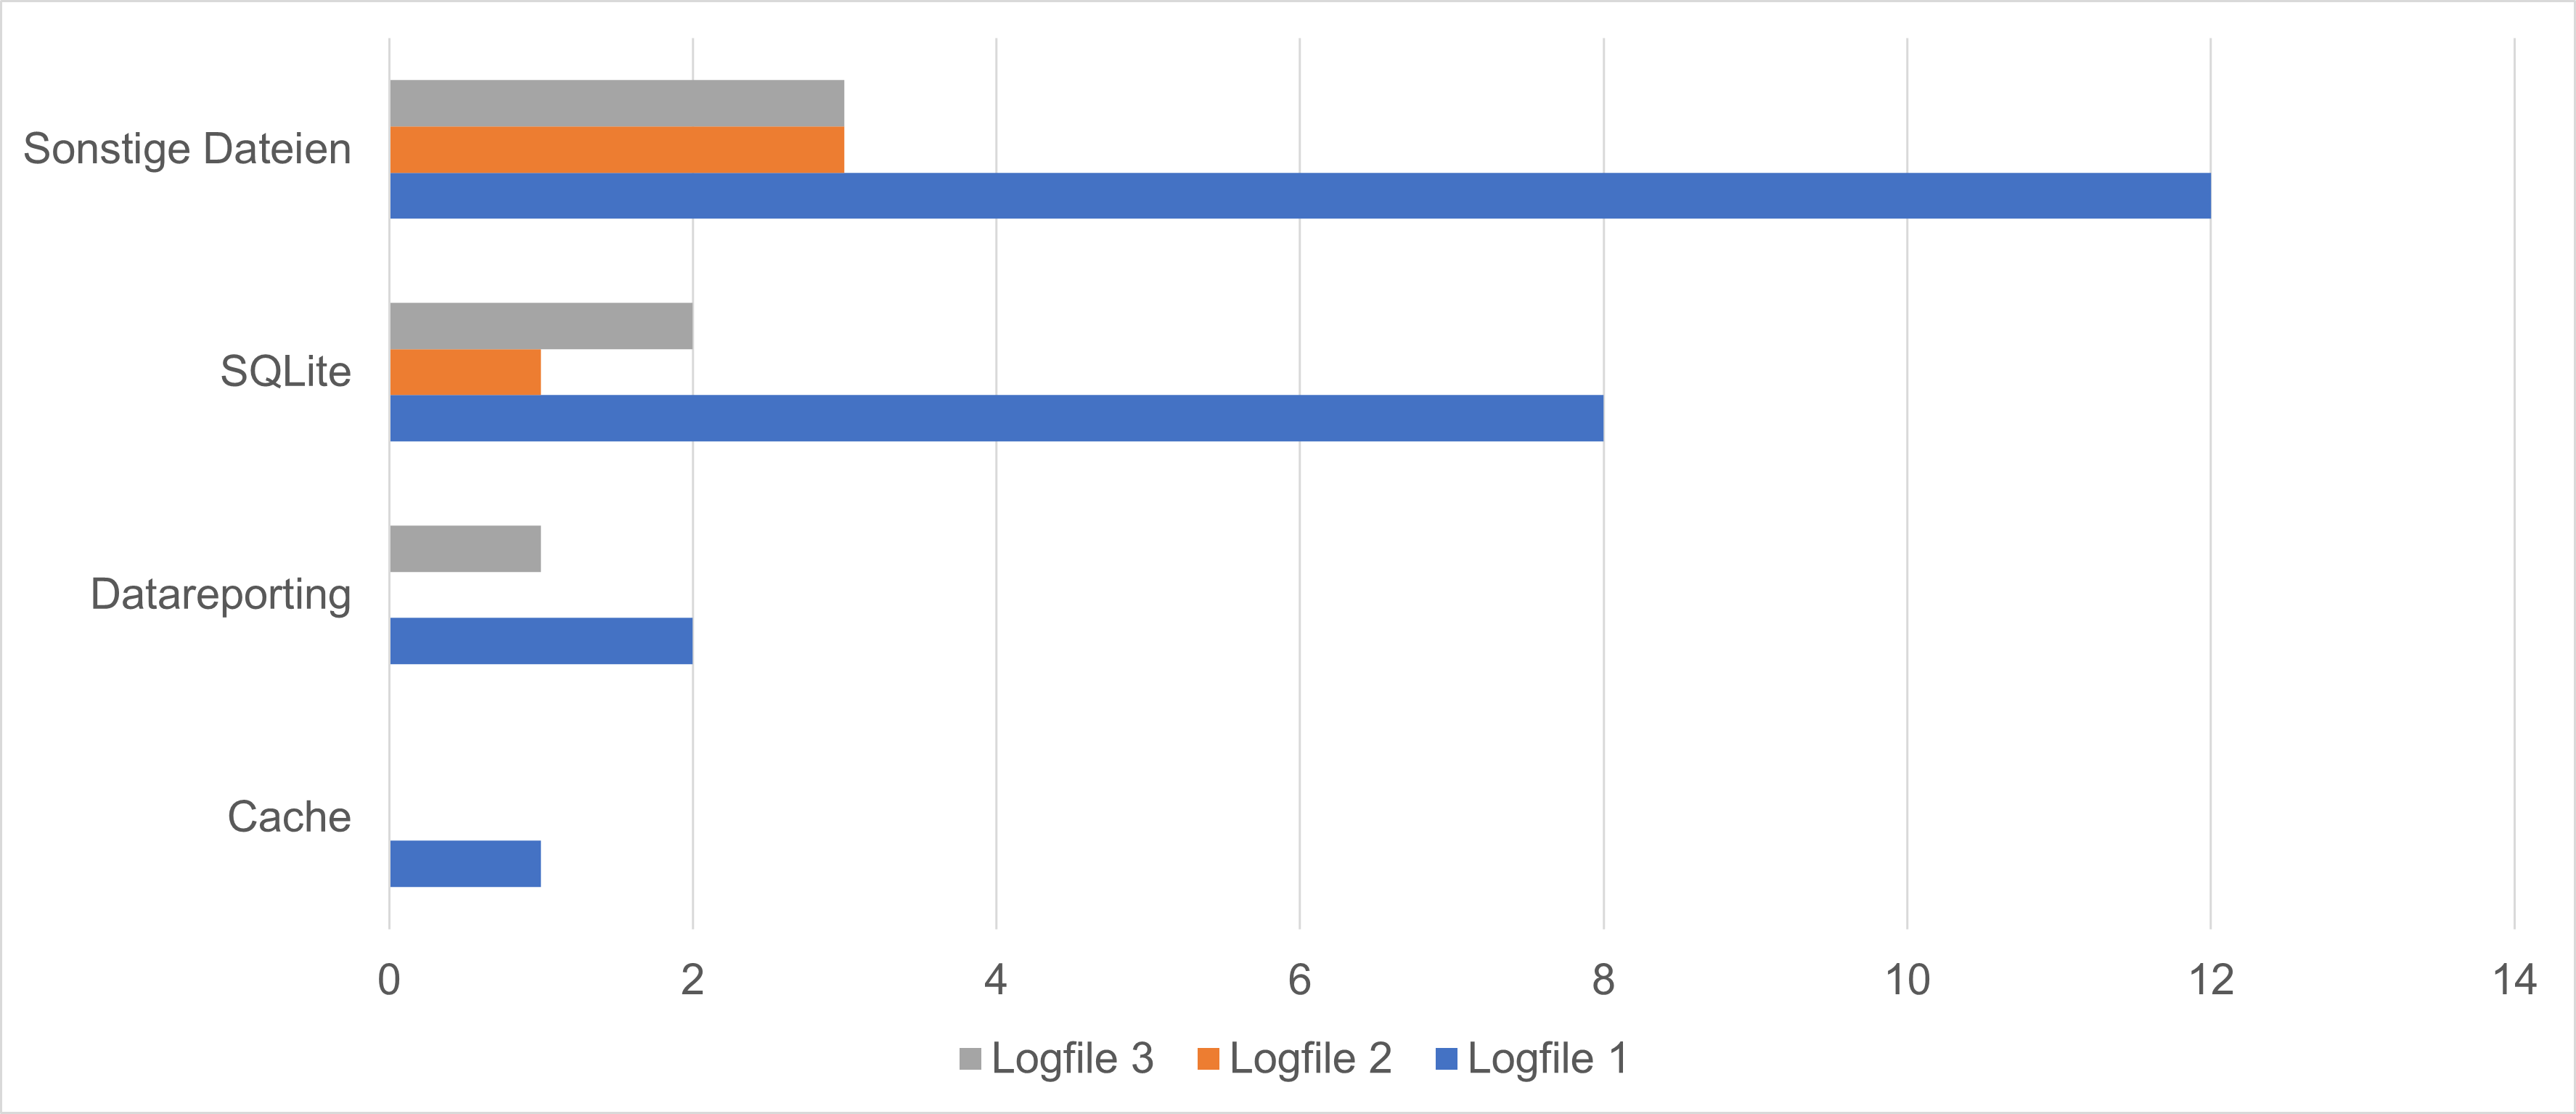
\includegraphics{bilder/tor-bar-chart-logfile1vs2cs3.png}}}
		\label{chart:final-criteria}  
		\caption{Comparison of found PB artifacts between RAM Dumps}
	\end{figure}

%Literatur:
%	o no traces were found in “common locations” \cite{Montasari.2015}
%		>  “places.sqlite”, “webappsstore. sqlite”, “sessionstore.bak”, “search.json” and “nssckbi.dll”
%	o	Safebrowsing: Alle Dateien in /safebrowsing-updating/ nicht relevant. Dort nur .vlpset und .sbstore Dateien. Speichern 256-Bit Hash von URLs, die auf SafeSearch Blacklist stehen 
%	o	Cache-Dateien: drei Caches: startupCache, jumpListCache (beide enthalten Binärdateien ohne Browsing Artefakte) und cache2 (können mit MozillaCacheView untersucht werden, enthalten keine Browsing Artefakte)
%	o	SQLite Datenbanken: Sqlite Dateien erst ohne WAL Dateien untersuchen, Danach mit sqlite3 Konsole: WAL in Datenbank schreiben mit: PRAGMA wal\_checkpoint; places.sqlite besonders relevant, da dort Browser in public Modus Browsing URLs verwaltet (Am besten hier vergleich mit Public Browsing machen)	
%		> \cite{Fayyad.2021} for Mozilla Firefox, 7 database files were recovered: cookies.sqlite-shm, places.sqlite-shm, prefs.js etc.
%		> \cite{Muir.2019} The two SQLite databases used by Firefox to track cookies and history (cookies.sqlite und places.sqlite) were both recoverable from the file system after deletion	
%		Ergebnisse stehen im Gegensatz zu \cite{Hedberg.2013} :
%			o	Chrome und Firefox: Einträge in places.sqlite + history.sqlite DB gefunden während PB! (Noch aktuell??)
%		Sonderfall: SQlite DB-Crash \cite{Hedberg.2013}
%			> WAL Files/Journal Files bei Crash gefunden -> Kann genutzt werden um zu beweisen, dass privater Browser genutzt wurde
%			> Daher: WAL Rollback mit sqlite3	
%	o	Jsonlz4 \& balkz4: Enthalten komprimierte Firefox-Sessions, jsonlz4 Dateien können mit Tool "entkomprimiert" werden: https://www.jeffersonscher.com/ffu/scrounger.html


\subsection*{Registry}
> Process Monitor: SetValue Operationen von Browser 
	Kategorien Registry Keys: Analog zu Firefox
	1) PreXULSkeletonUISettings:
		> Prefix: Absoluter Installationspfad von Firefox
		> Skeleton UI Einstellungen von Firefox % https://itigic.com/skeleton-ui-new-firefox-interface-to-start-up-much-faster/#google_vignette
			Definition:
				> Der "PreXULSkeletonUISettings" Registry Key enthielt Einstellungen für die Benutzeroberfläche (UI) des Firefox-Browsers, insbesondere für das sogenannte "Skeleton UI". Das Skeleton UI ist eine vereinfachte Benutzeroberfläche, die während des Ladens des Browsers angezeigt wird, bevor die vollständige Benutzeroberfläche geladen ist. Es besteht aus grundlegenden Steuerelementen und Elementen, die dem Benutzer die Interaktion ermöglichen, während der Rest der Benutzeroberfläche noch geladen wird.
				> Der "PreXULSkeletonUISettings"-Schlüssel enthielt Konfigurationsoptionen wie Farben, Positionen und andere Einstellungen für das Skeleton UI. Durch das Bearbeiten dieses Schlüssels konnten Benutzer die Darstellung des Skeleton UI anpassen. Es ist jedoch wichtig zu beachten, dass das Ändern der Registrierungseinträge ein fortgeschrittenes Verfahren ist und Fehler zu Problemen mit dem Browser führen kann.
			
		> Struktur der Keys: % HKCU\SOFTWARE\Mozilla\Firefox\PreXULSkeletonUISettings\C:\Program Files\Mozilla Firefox\firefox.exe|<UI Einstellung>
		> Unterschiedliche UI Einstellungen
			- % ScreenX (DWORD)
			- % ScreenY (DWORD)
			- % Width (DWORD)
			- % Height (DWORD)
			- % Maximized (DWORD)
			- % Flags (DWORD)
			- % CssToDevPixelScaling (REG_BINARY)
			- % UrlbarCSSSpan (REG_BINARY)
			- % SearchbarCSSSpan (REG_BINARY)
			- % SpringsCSSSpan (REG_BINARY)
		> keine PB Artefakte unter UI Einstellungen	
	2) Business Activity Monitoring % https://learn.microsoft.com/de-de/biztalk/core/business-activity-monitoring-bam
		> Quelle: % https://notes.qazeer.io/dfir/windows/_artefacts_overview
		> BAM is a mostly undocumented feature that controls the programs executed in the background. DAM is a feature for devices supporting the "Connected Standby" mode (i.e when a device is turned on, but its display will be turned off). As a result, the BAM registry keys will contain data on any devices, while DAM registry keys will only contain data on mobile devices.
		> The BAM registry key contains multiple subkeys under bam\\State\\UserSettings, with one subkey per user, identified with the user SID. While the key is in the SYSTEM registry hive, program executions can thus still be tied to a specific user using this SID.
		> Each user-specific key contains a list of executed programs, with their full path and timestamp of last execution.
		> If a file is deleted, the eventual associated entry in the BAM is deleted as well after the system reboot. Additionally, BAM entries older than 7 days are deleted upon system boot. The BAM thus provides limited information on historic execution of programs
		> No entries are created in the BAM keys for executables on removable media and/or on network shares.
		> Key: %  HKLM\System\CurrentControlSet\Services\bam\State\UserSettings\S-1-5-21-588412547-2749917301-3803556669-1001\\Device\HarddiskVolume2\Program Files\Mozilla Firefox\firefox.exe (REG_BINARY)

Quantitativ: (Diagramme)
	- Stacked Balkendiagramm jeweils für Logfile 1 und Logfile2: Anteil Kategorie 1 bzw.2 an allen Registry-Schreiboperationen
	\begin{figure}[h!]
		\centerline{\resizebox{\linewidth}{!}{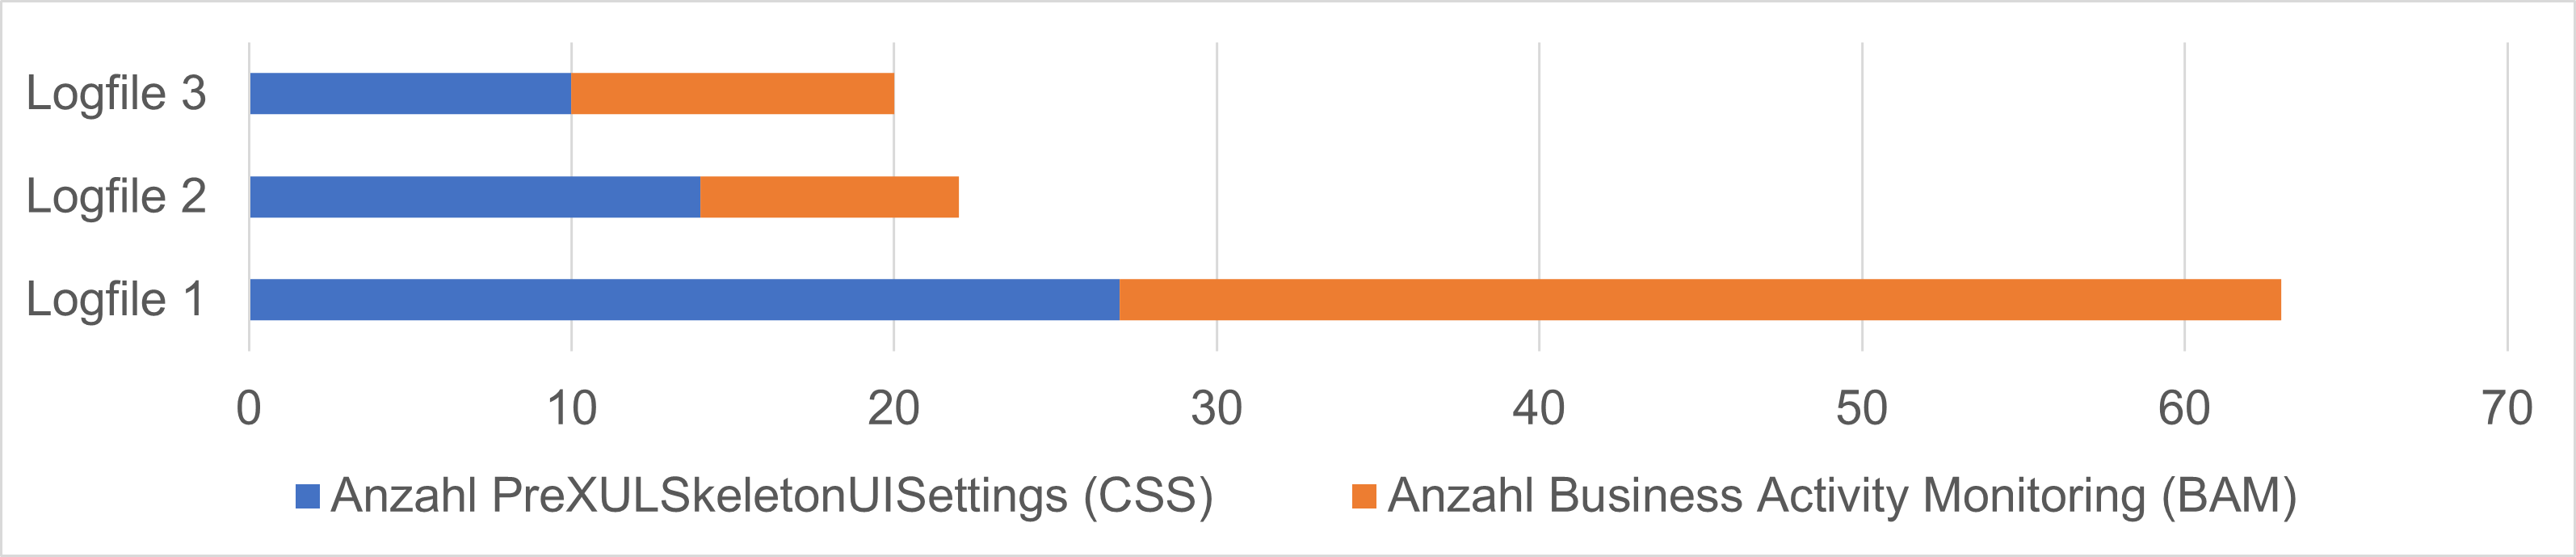
\includegraphics{bilder/tor-registry-stacked-bar-chart.png}}}
		\label{chart:final-criteria}  
		\caption{Comparison of found PB artifacts between RAM Dumps}
	\end{figure}
	
> Stringsuche in Registry Hives mit Registry Explorer (Siehe Liste)
	In allen Hives kein Treffer für alle Suchbegriffe

Literatur: 
	> Wie bei Firefox: Shellactivities Key existiert nicht mehr --> Nicht mehr vorhanden in aktueller Version (Verweis auf E-Mail)

%Literatur:
%	>	Auf Autor verweisen: angeblich in Shellactivities Ergebnisse. --> Nicht mehr vorhanden in aktueller Version (Verweis auf E-Mail)
%	>	Process Monitor/Regshot zeigen keine relevanten Key-Änderungen
%	> \cite{Muir.2019}: Autopsy Keyword Suche nach Suchbegriffen: Ergebnisse in \%SystemRoot\%Minidump NTUSER.DAT, ntuser.dat.LOG1 (a log of changes to NTUSER.DAT)
%	> Zentral: shellactivites Key:	NTUSER.DAT --> “shellactivities” key \cite{Muir.2019}
%	> \cite{Rochmadi.2017} Detection of registry changes helps to determine what the appropriate plugin is used to search for digital evidence using volatility memory forensic:
%	- RegQueryValue:	HKCU/Software/Microsoft/Windows/CurrentVersion/InternetSettings/Connections/DefaultConnectionSettings
%	- RegCloseValue: 	HKCU/Software/Microsoft/Windows/CurrentVersion/InternetSettings/Connections
%	- IRP\_MJ\_READ: C:/pagefile.sys

\subsection*{Black-Box Analyse/Uncommon Locations}

\subsubsection*{Analyse mit Autopsy}
Bei White-Box Analyse/Common Locations: Autopsy nur zur Dateiextraktion genutzt, hier: als konkretes forensisches Werkzeug

Stichwortsuche:
- In allen Snapshots keine Treffer (auch innerhalb \$Carved)
- TODO: Pagefile gefunden?

Von Autopsy automatisch indexierte Dateien: 
In allen Fällen: keine Dateien gelöscht, nur über Zeitraum der Snapshots neue dazugekommen
- Web Bookmarks:
	\begin{figure}[h!]
		\centerline{\resizebox{\linewidth}{!}{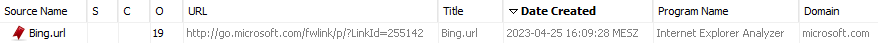
\includegraphics{bilder/cfv_tor_autopsy_web_bookmarks.png}}}
		\label{chart:final-criteria}  
		\caption{Autopsy Web Bookmarks}
	\end{figure}
	Snapshot 1:
		> Bing.url (Unter C:/User/Forensik/Favorites/Links) enthält Bing Startseite
	Snapshot 2:
		> unverändert zu 1
	Snapshot 3-1:
		> unverändert zu 2
	Snapshot 3-2:	
		> unverändert zu 3-1
	Snapshot 4:
		> unverändert zu 3-2
- Web Cookies:
	\begin{figure}[h!]
		\centerline{\resizebox{\linewidth}{!}{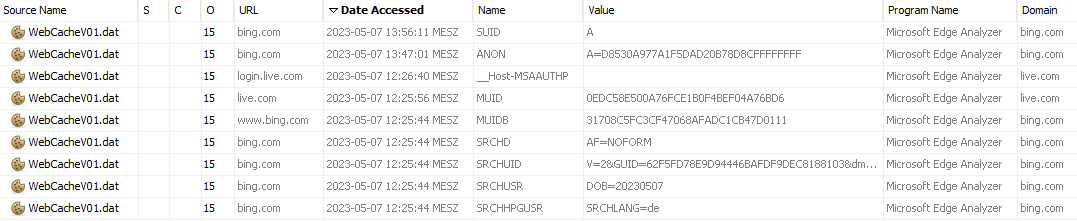
\includegraphics{bilder/cfv_tor_autopsy_web_cookies.png}}}
		\label{chart:final-criteria}  
		\caption{Autopsy Web Cookies}
	\end{figure}
	Snapshot 1:
		> 9 Einträge in WebCacheV01.dat (= DB des Internet Explorers zum speichern von Browserdaten): Cookies für bing.com und live.com (= outlook)
	Snapshot 2:
		> unverändert zu 1
	Snapshot 3-1:
		> unverändert zu 2
	Snapshot 3-2:
		> unverändert zu 3-1
	Snapshot 4:
		> unverändert zu 3-2
- Web History:
	\begin{figure}[h!]
		\centerline{\resizebox{\linewidth}{!}{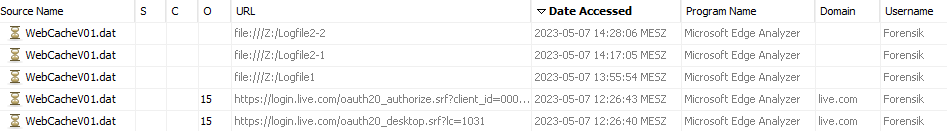
\includegraphics{bilder/cfv_tor_autopsy_web_history.png}}}
		\label{chart:final-criteria}  
		\caption{Autopsy Web History}
	\end{figure}
	Snapshot 1:
		> 2 Einträge in WebCacheV01.dat:
			- 2x live.com (= outlook)
	Snapshot 2:
		> 1 neuer Einträge in WebCacheV01.dat:
			- file:///Z:/Logfile\_1 (= Process Monitor Logfile, die in shared-Folder geladen wurde) -> Erklärung?
	Snapshot 3-1:
		> 1 neuer Eintrag in WebCacheV01.dat:
			- file:///Z:/Logfile\_2-1 (= Process Monitor Logfile, die in shared-Folder geladen wurde) -> Erklärung?
	Snapshot 3-2:
		> 1 neuer Eintrag in WebCacheV01.dat:
			- file:///Z:/Logfile\_2-2 (= Process Monitor Logfile, die in shared-Folder geladen wurde) -> Erklärung?
	Snapshot 4:
		> unverändert zu 3-2
- Web Categories:
	\begin{figure}[h!]
		\centerline{\resizebox{\linewidth}{!}{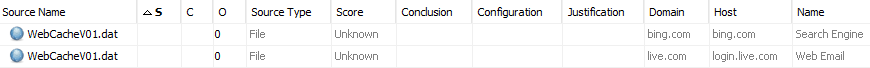
\includegraphics{bilder/cfv_tor_autopsy_web_categories.png}}}
		\label{chart:final-criteria}  
		\caption{Autopsy Web Categories}
	\end{figure}
	Snapshot 1:
		> 2x WebCacheV01.dat aufgelistet => Mit HxD untersucht, keine PB Artefakte
	Snapshot 2:
		> unverändert zu 2
	Snapshot 3-1:
		> unverändert zu 3
	Snapshot 3-2:
		> unverändert zu 3-1
	Snapshot 4:
		> unverändert zu 3-2
		
Zusammenfassung:
- keine PB Artefakte
- Keine neuen Erkenntnisse vgl. mit intensiver Analyse mittels Process Monitor in Kapitel X
- .onion URL Einträge in places.sql nicht erkannt

%Literatur:
%	o	Autopsy Keywortsuche: 
%		>	In alles Snapshots ergebnislos (keine Keyword-Hits
%		-->	In Literatur: Autoren fanden Ergebnisse in pagefile.sys 
%			> Autopsy: websites and some of the keywords found in hidden file called “pagefile.sys” \cite{Mahlous.2020}
%			o \cite{Montasari.2015} traces were found in: 
%				> However, on investigating the “pagefile.sys”, some entries were discovered
%				> Using the “data carving” technique, profile picture was recovered
%			o \cite{Said.2011} 
%				> Examining pagefile.sys showed some positive hits 			
%		--> Evtl. hier zeigen, was gefunden werden kann, wenn RAM reduziert
%		--> Aber auf Problem hinweisen, dass gefundener String in pagefile nicht direkt Browser zugeordnet werden kann
%		> \cite{Gabet.2018}	Firefox only produced three recoverable artefacts as reported by both tools (FTK, Autopsy) --> Artefakte werden nicht genannt!
%		> \cite{Muir.2019} Autopsy Keyword Suche nach Suchbegriffen: unallocated space
%		> Autopsy Carving Module (\$Carved): \cite{Muir.2019}
%			•	When searching for the string ’clot’ from the browsing protocol, six .dll, .edb and .reg files were discovered in unallocated space.
%			•	Further searching of unallocated space uncovered references to the Tor installation directory and the obfs4 bridging IP addresses
%			•	browsing data found in NTUSER.DAT was also replicated in unallocated space.
%	o	Autopsy PlugIns:
%		>	*** TODO: Hier Liste mit PlugIns ***

\subsubsection*{Analyse mit Volatility}
Vorgehen: Siehe "Methodik" Kapitel
	- Ausgangslage: Volatility Yarascan Treffer
	- Für jeden Treffer: virtueller Offset des Strings, PID, getriggerte Yararule, getriggerte Yara Component z(= Variablenname des gesuchten Strings), gefundener String
	- Neue Spalte: "Prozessname" -> zu jeder PID Prozessnamen
	- Ergebnisse Aufbereitet nach folgendem Schema:
		> Für jeden RAM Dump
		> Für jede Yararule
		> Für jede Component
		> Filter: Prozessname = Firefox -> Anzahl zählen
		> Filter: Prozessname = Alle Prozesse außer Firefox -> Anzahl zählen

Wie bei Firefox: HTML Artefakte wurden in keinem RAM Dump gefunden => Nicht aufgeführt

Yararule "Keyword":
	\begin{figure}[h!]
		\centerline{\resizebox{\linewidth}{!}{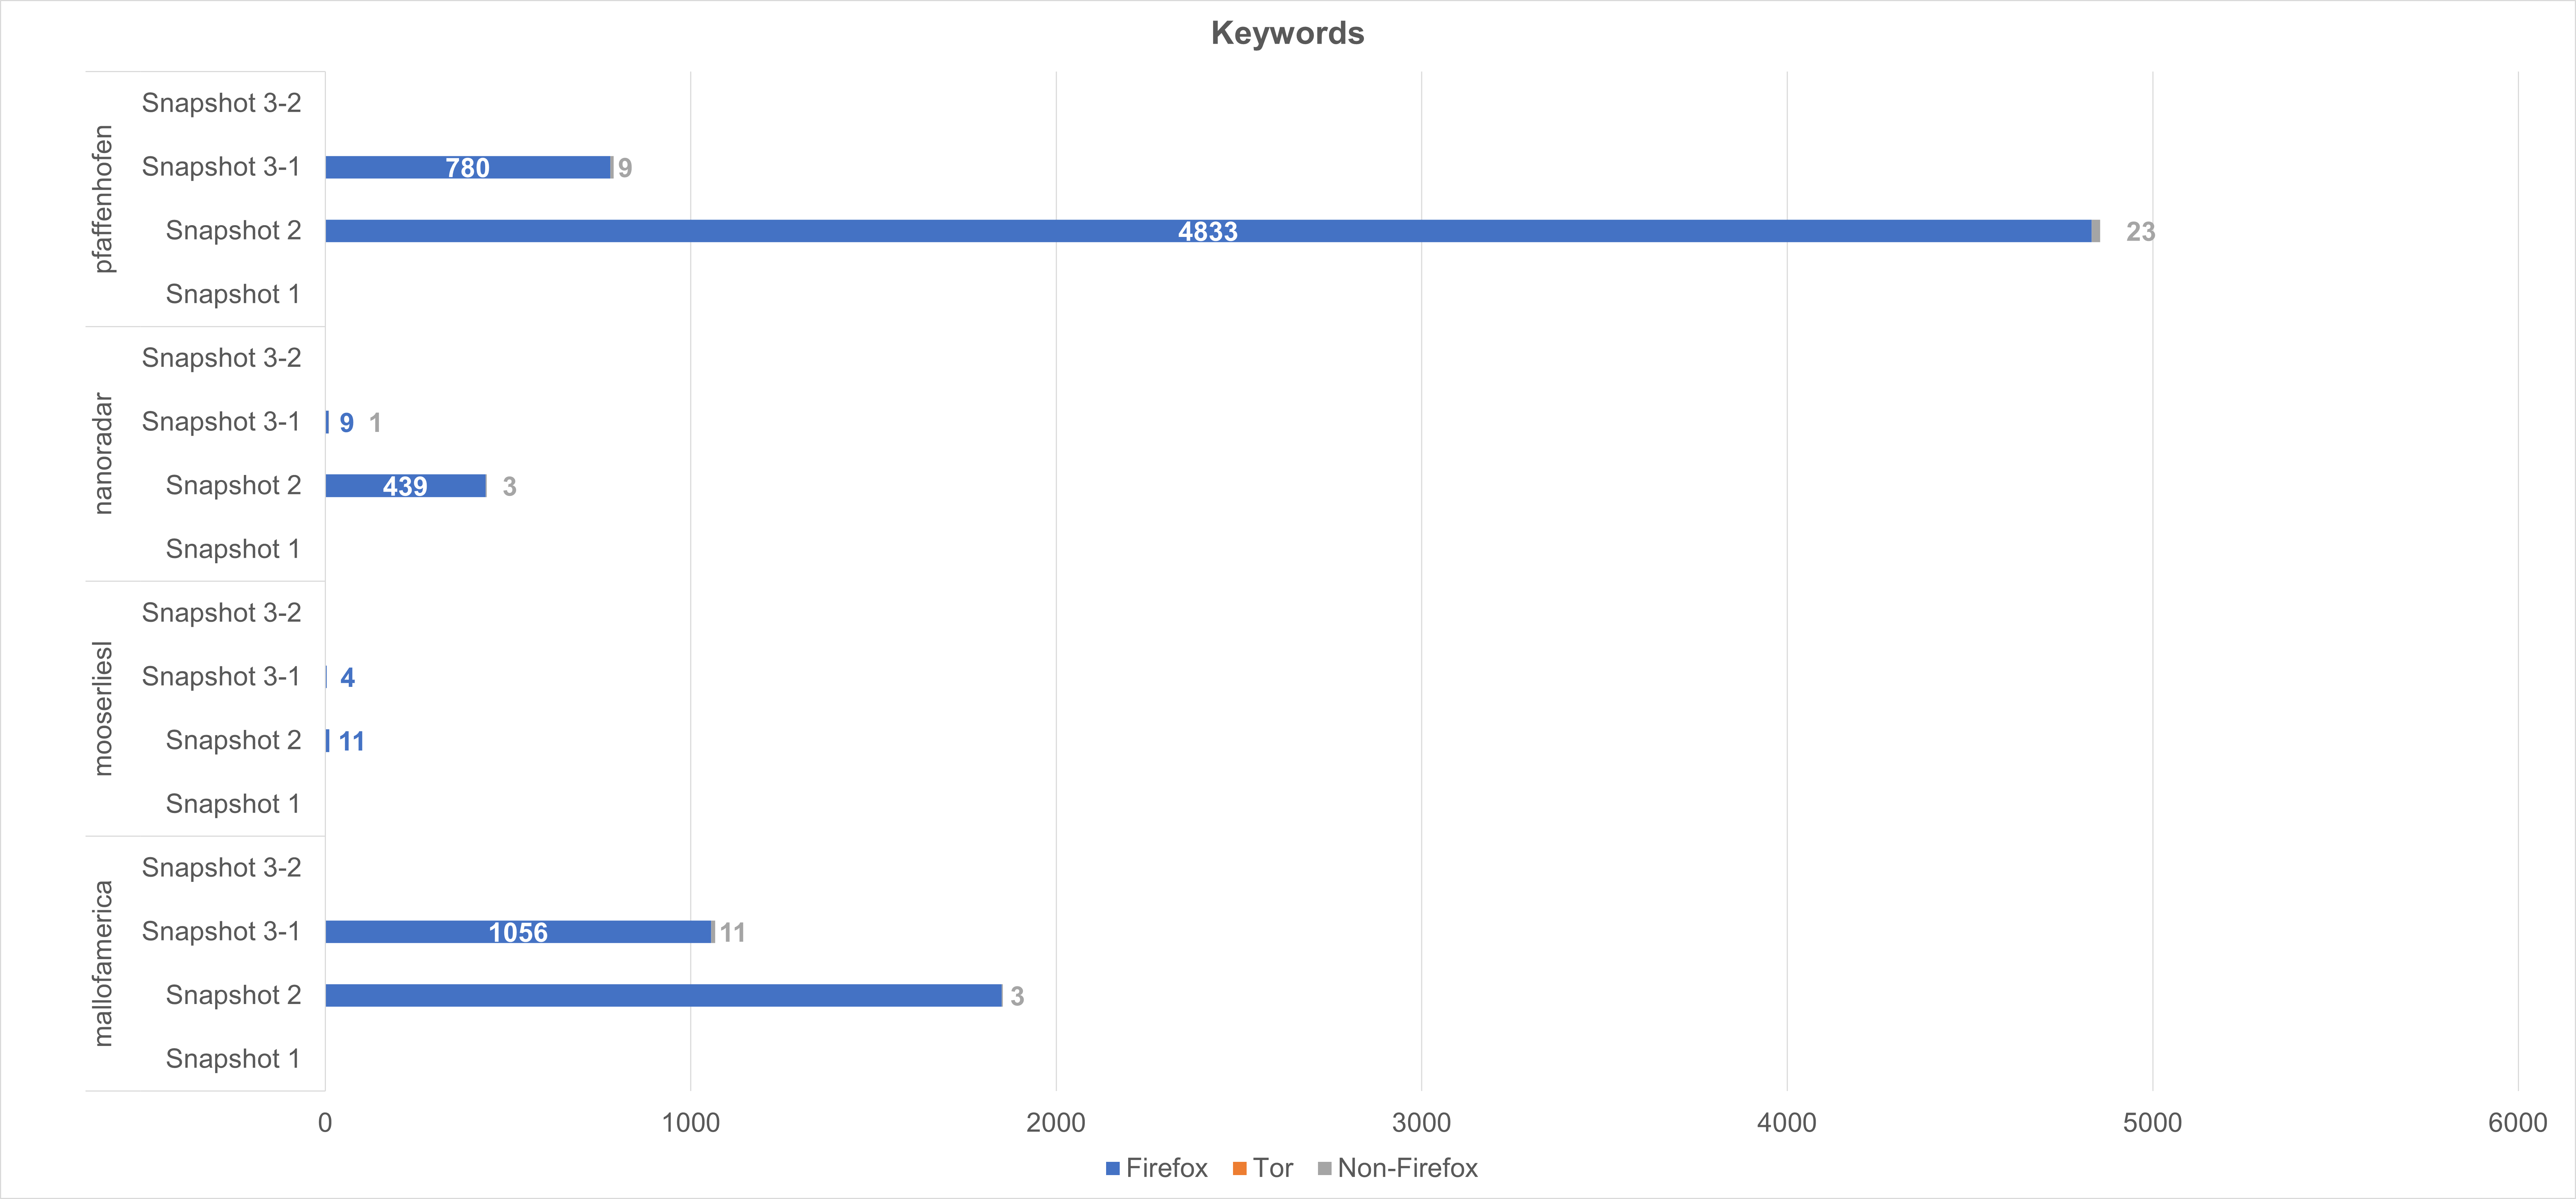
\includegraphics{bilder/volatility/tor/keywords.png}}}
		\label{chart:final-criteria}  
		\caption{Keywords}
	\end{figure}
	Analyse:
		> Ausschließlich in RAM Dump 2 und RAM Dump 3-1 Keyword Artefakte gefunden
		> In RAM Dump 3-1 bei jedem Keyword deutlich weniger Artefakte als in RAM Dump 2 => Identitäts-Reset reduziert Keyword Artefakte deutlich
		> Hauptsächlich in Firefox Prozess, kein Artefakt in Tor.exe Prozess
		> Mit 4833 Artefakten in RAM Dump 2 am häufigsten "pfaffenhofen" vertreten. Vermutung: Evtl. weil Google Maps viele zusätzliche Artefakte lädt. 
		> Nach Schließen von Tor Browser: keine Keyword Artefakte mehr in RAM
		
Yararule "URL":
	\begin{figure}[h!]
		\centerline{\resizebox{\linewidth}{!}{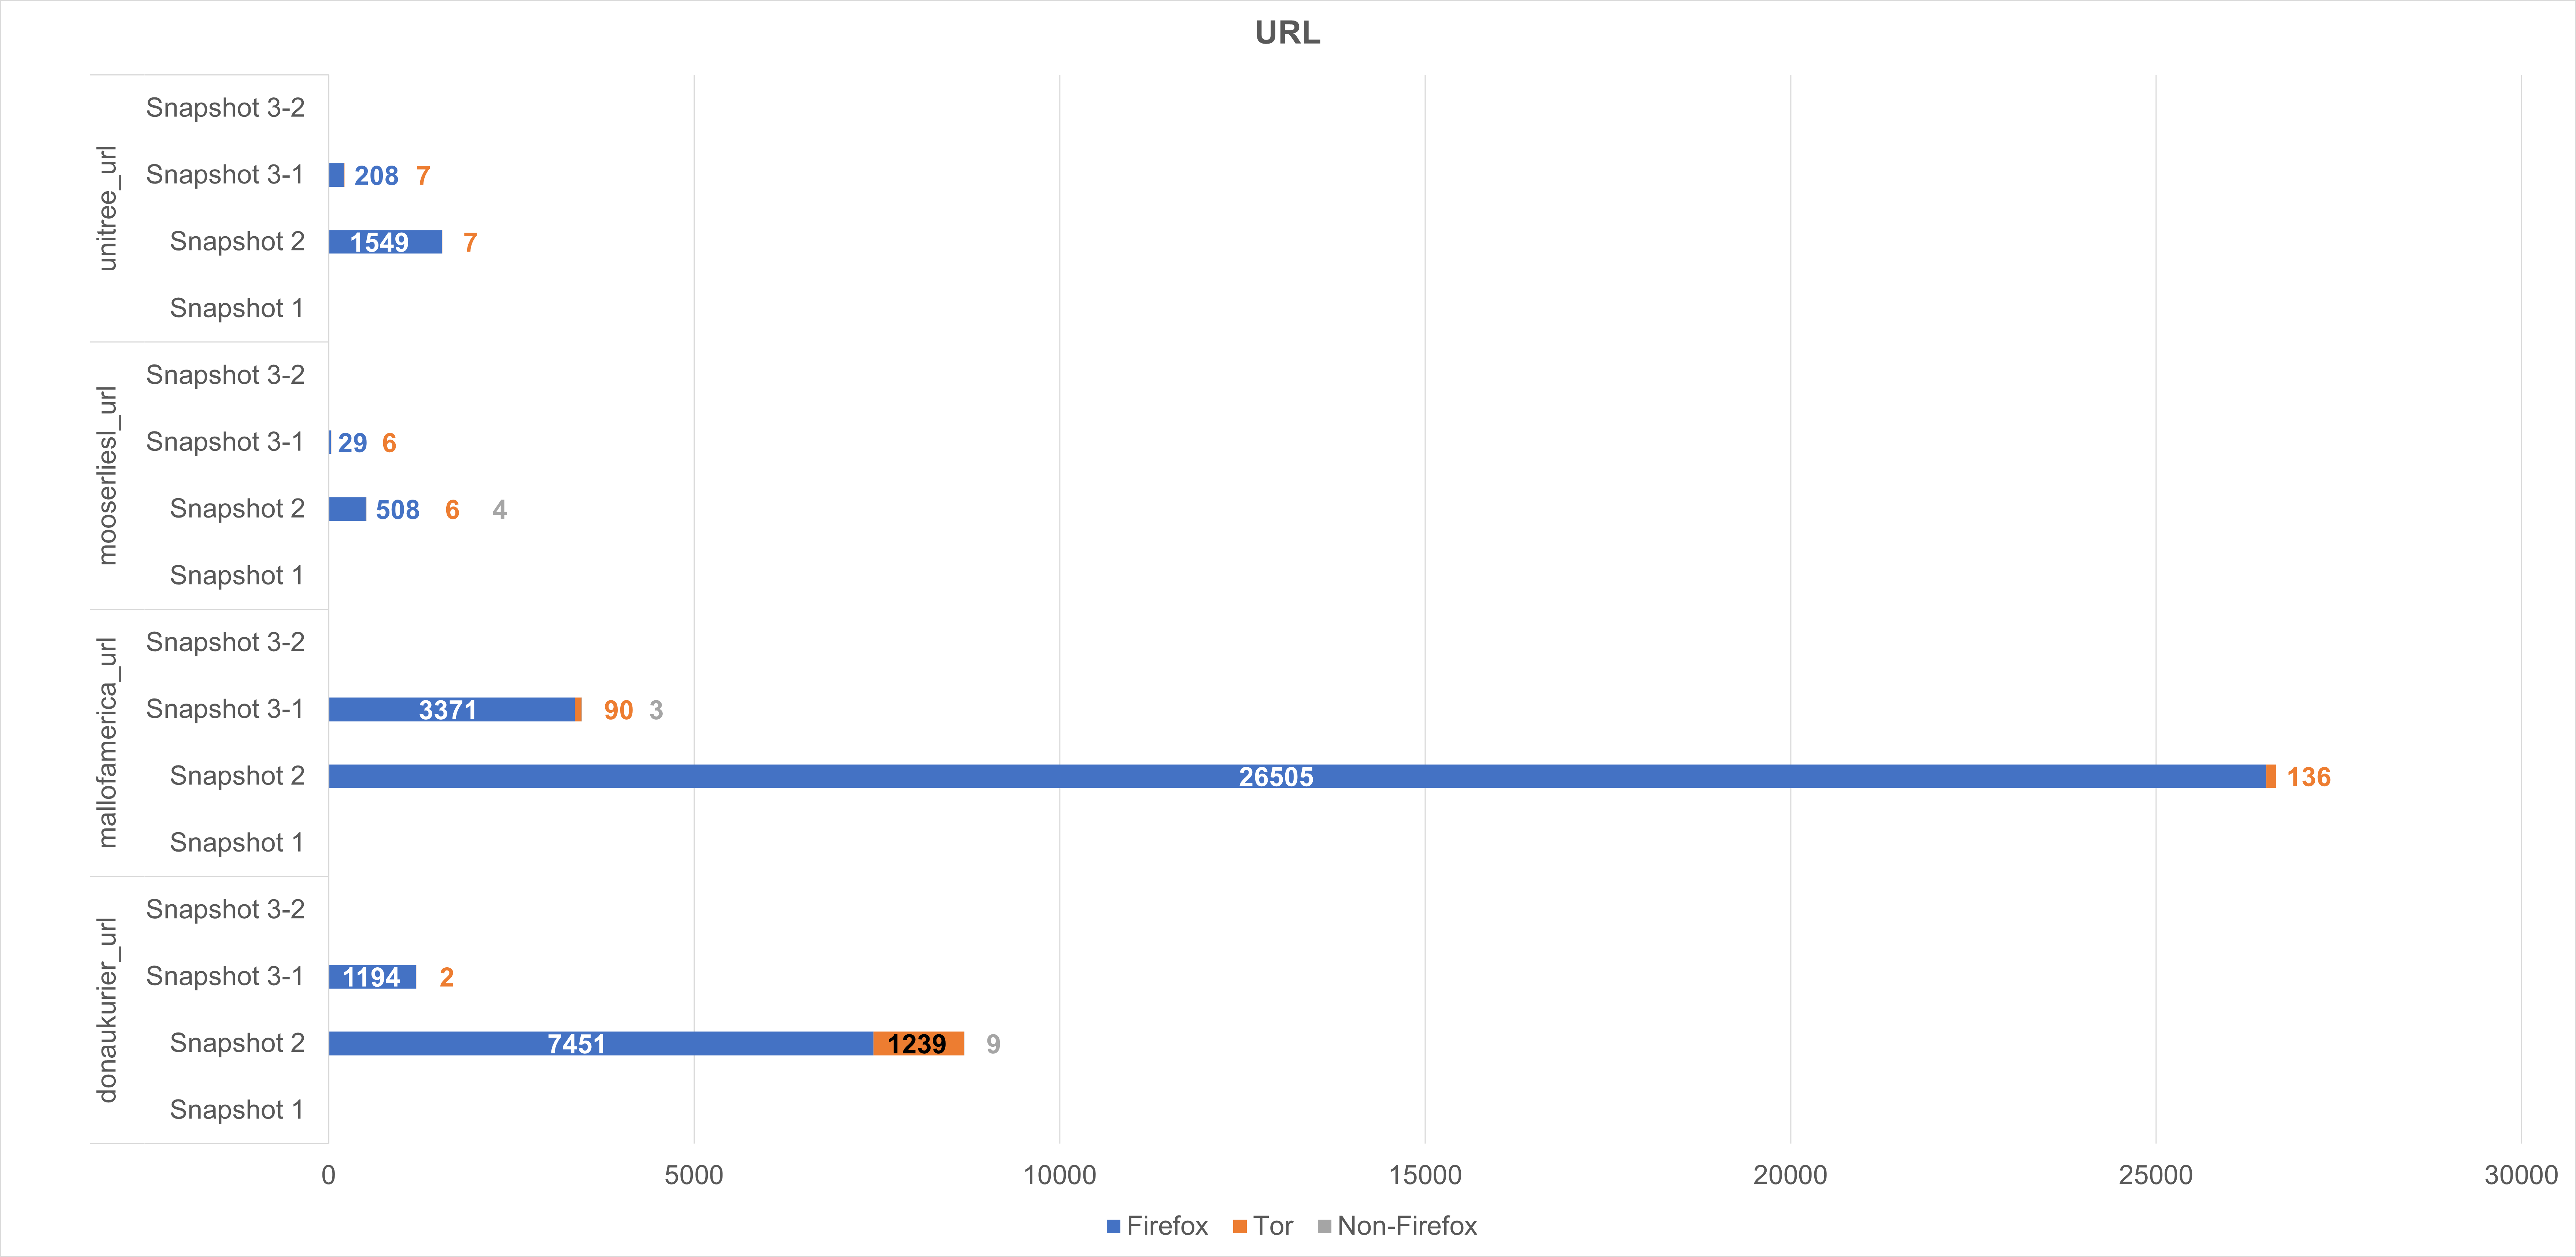
\includegraphics{bilder/volatility/tor/url.png}}}
		\label{chart:final-criteria}  
		\caption{URL}
	\end{figure}
	Analyse:
		> Wie bei Yararule "Keyword": Ausschließlich in RAM Dump 2 und RAM Dump 3-1 Keyword Artefakte gefunden
		> In RAM Dump 3-1 bei jedem Keyword deutlich weniger Artefakte als in RAM Dump 2 => Identitäts-Reset reduziert URL Artefakte deutlich
		> Hauptsächlich in Firefox Prozess, danach am häufigsten Tor.exe Prozess und am wenigsten Artefakte in anderen Prozessen
		> Bemerkenswert: "mallofamerica.com" ist mit 26.505 mal in RAM Dump 2 am häufigsten als Artefakt gefunden worden. Vergleich: "mooserliesl.de" wurde nur 508 mal in RAM Dump 2 gefunden
		> Nach Schließen von Tor Browser: keine URL Artefakte mehr in RAM
		
		> TODO: DNSCache?

Yararule "Mail":
	\begin{figure}[h!]
		\centerline{\resizebox{\linewidth}{!}{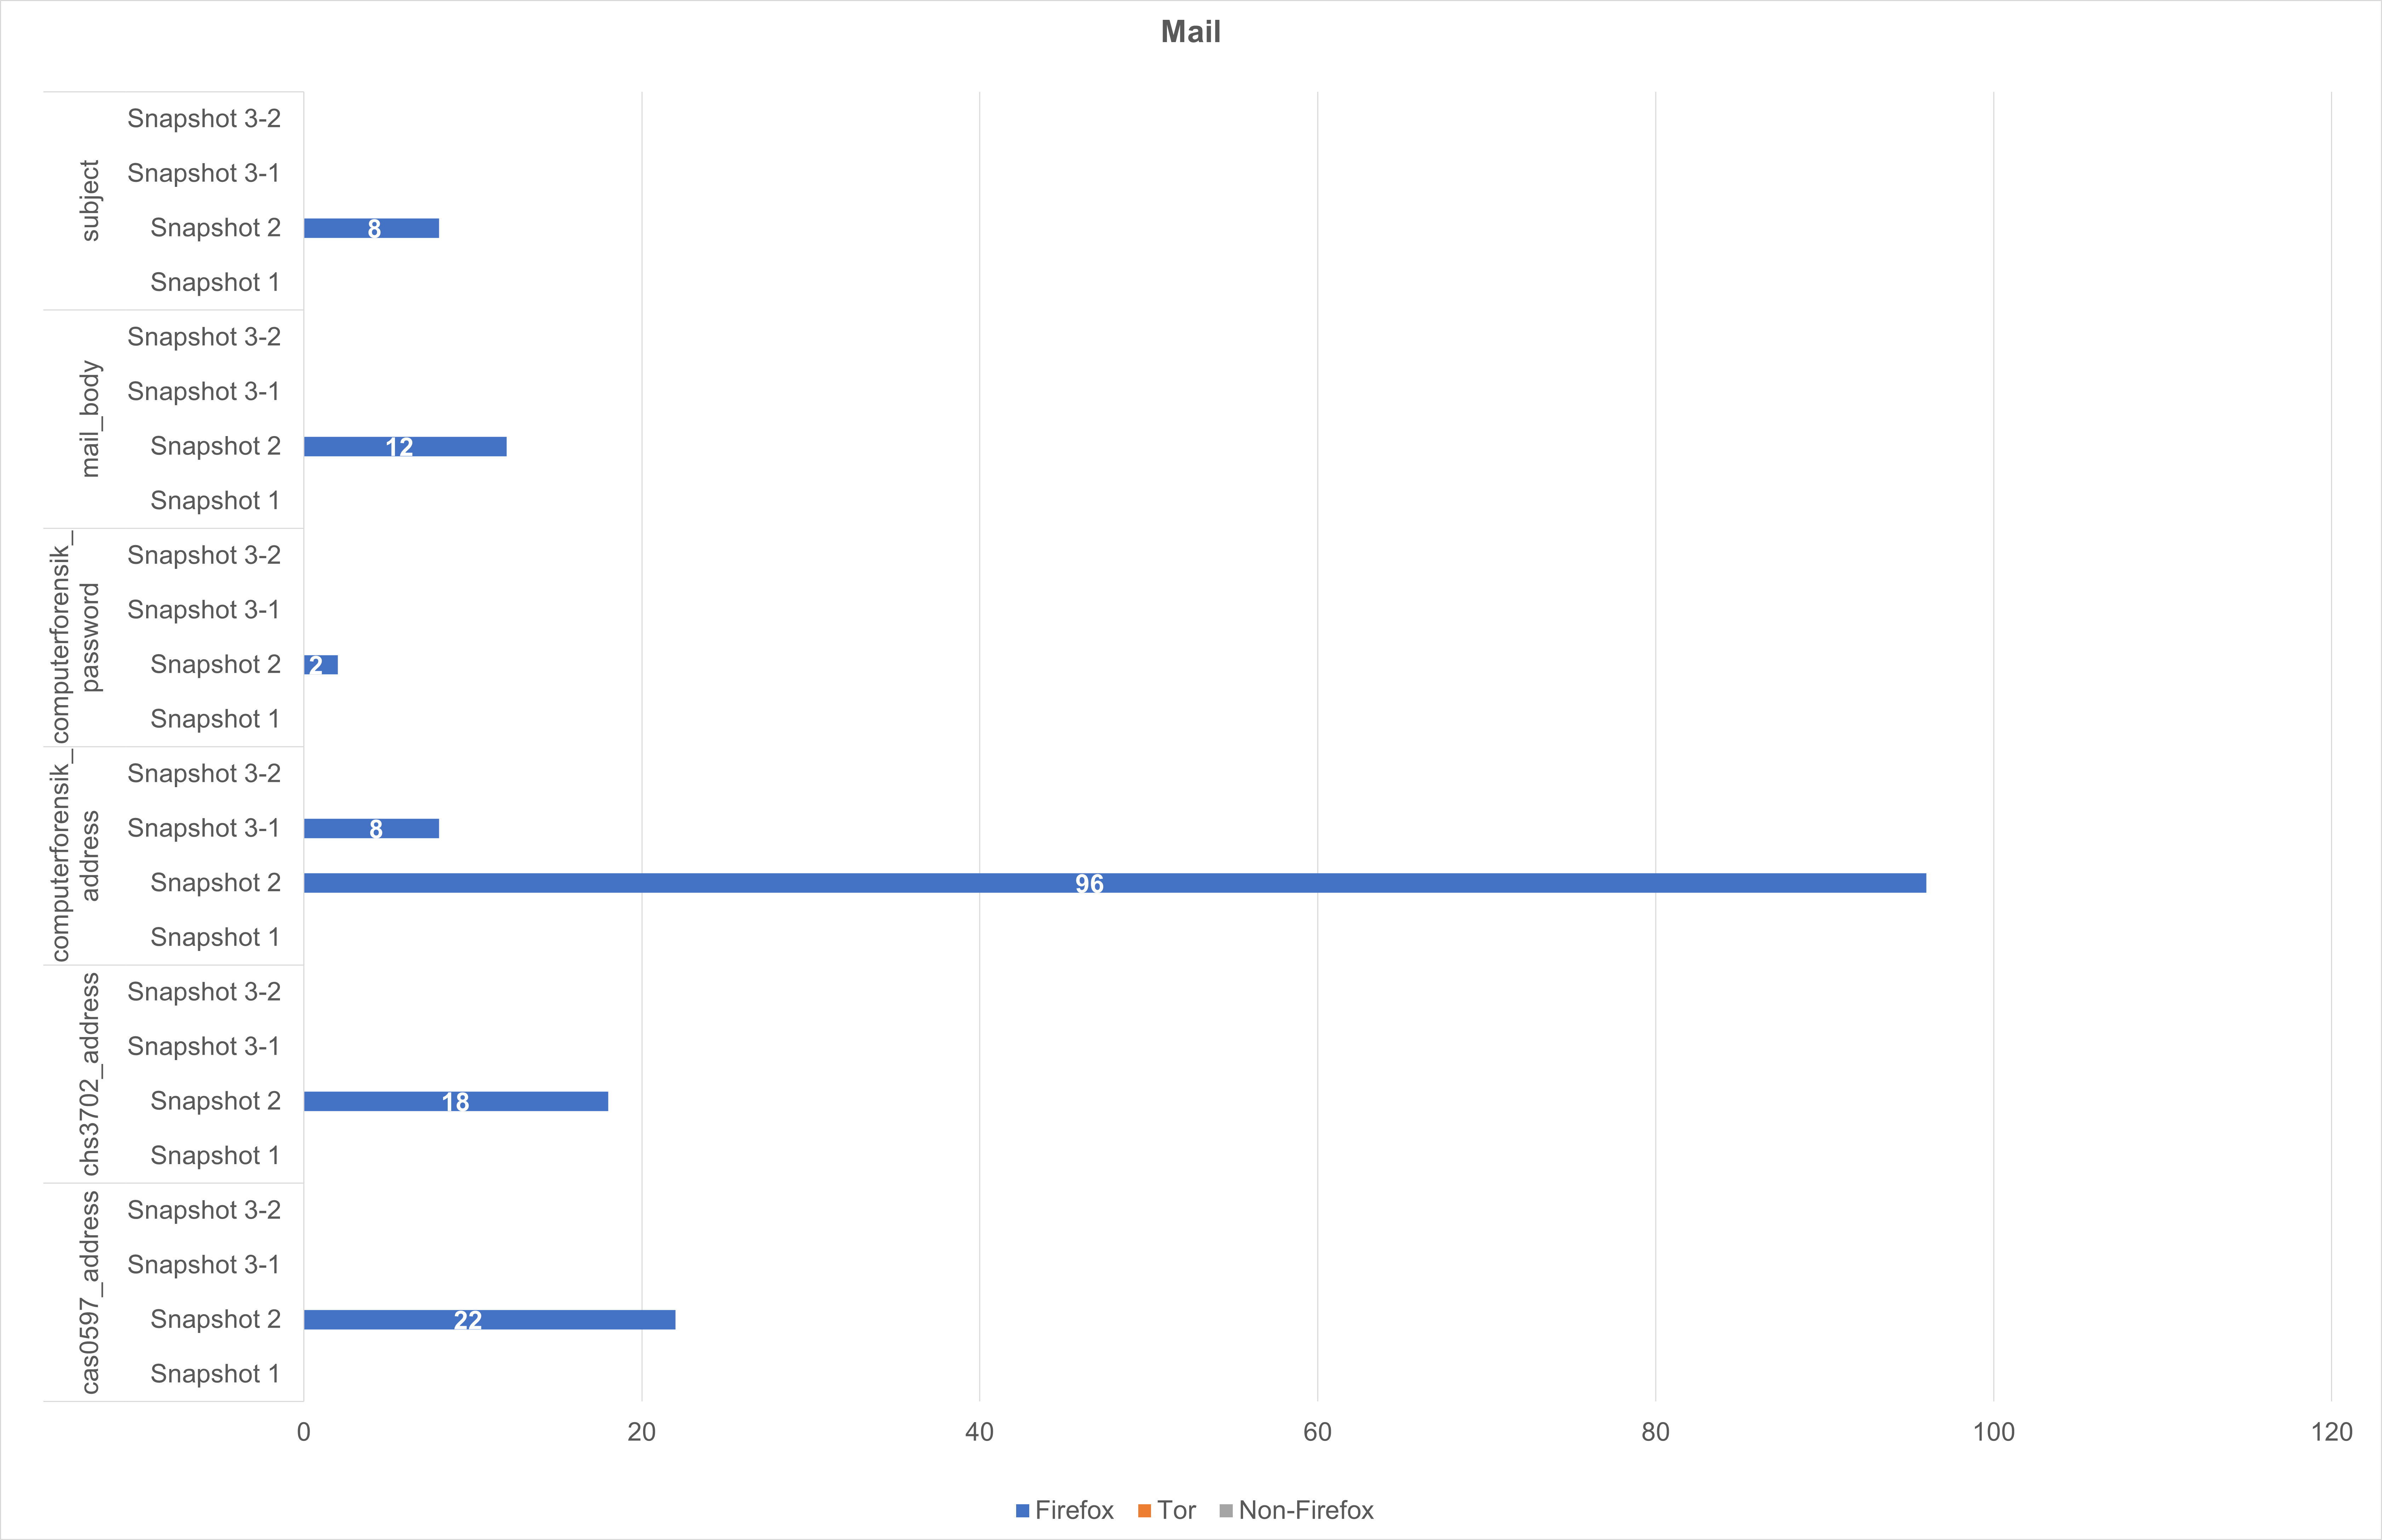
\includegraphics{bilder/volatility/tor/mail.png}}}
		\label{chart:final-criteria}  
		\caption{Mail}
	\end{figure}
	Analyse:
		> Alle Mail Artefakte gefunden
		> Artefakte ausschließlich in Firefox Prozess gefunden
		> Artefakte fast ausschließlich in RAM Dump 2 Mail gefunden
		> Nur die Absenderadresse "computerforensikvl@gmail.com" wurde nach Identitäts-Reset in RAM Dump 3-1 gefunden
		> Absenderadresse ist häufigstes Mail Artefakt
		> Bemerkenswert: Passwort wurde 2x als Klartext im RAM gefunden!
			String Kontext:
				Offsets:		PIDs:
				0xb9ce29180c8	7420
				0x2859f4ffd4e0	7420
				0x24083b41858	8424
				0x240840e5b08	8424
				
Yararule "Image":
	\begin{figure}[h!]
		\centerline{\resizebox{\linewidth}{!}{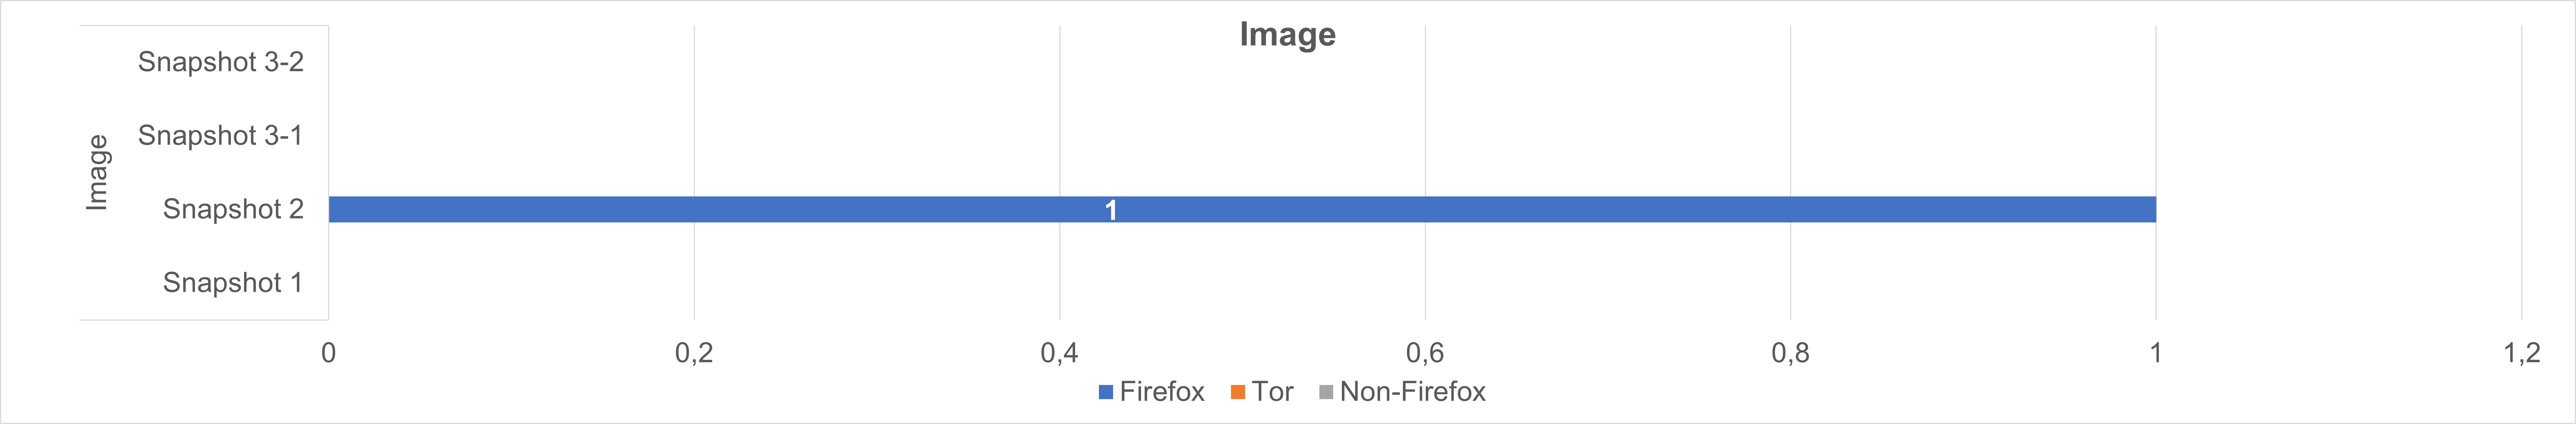
\includegraphics{bilder/volatility/tor/image.png}}}
		\label{chart:final-criteria}  
		\caption{Image}
	\end{figure}
	Analyse:
		> Hex-Wert von Donaukurier Bild wurde ein einzigees mal im 2. RAM Dump in einem Firefox Prozess gefunden
	

Zusammenfassung = Stacked Bar Chart:
\begin{figure}[h!]
	\centerline{\resizebox{\linewidth}{!}{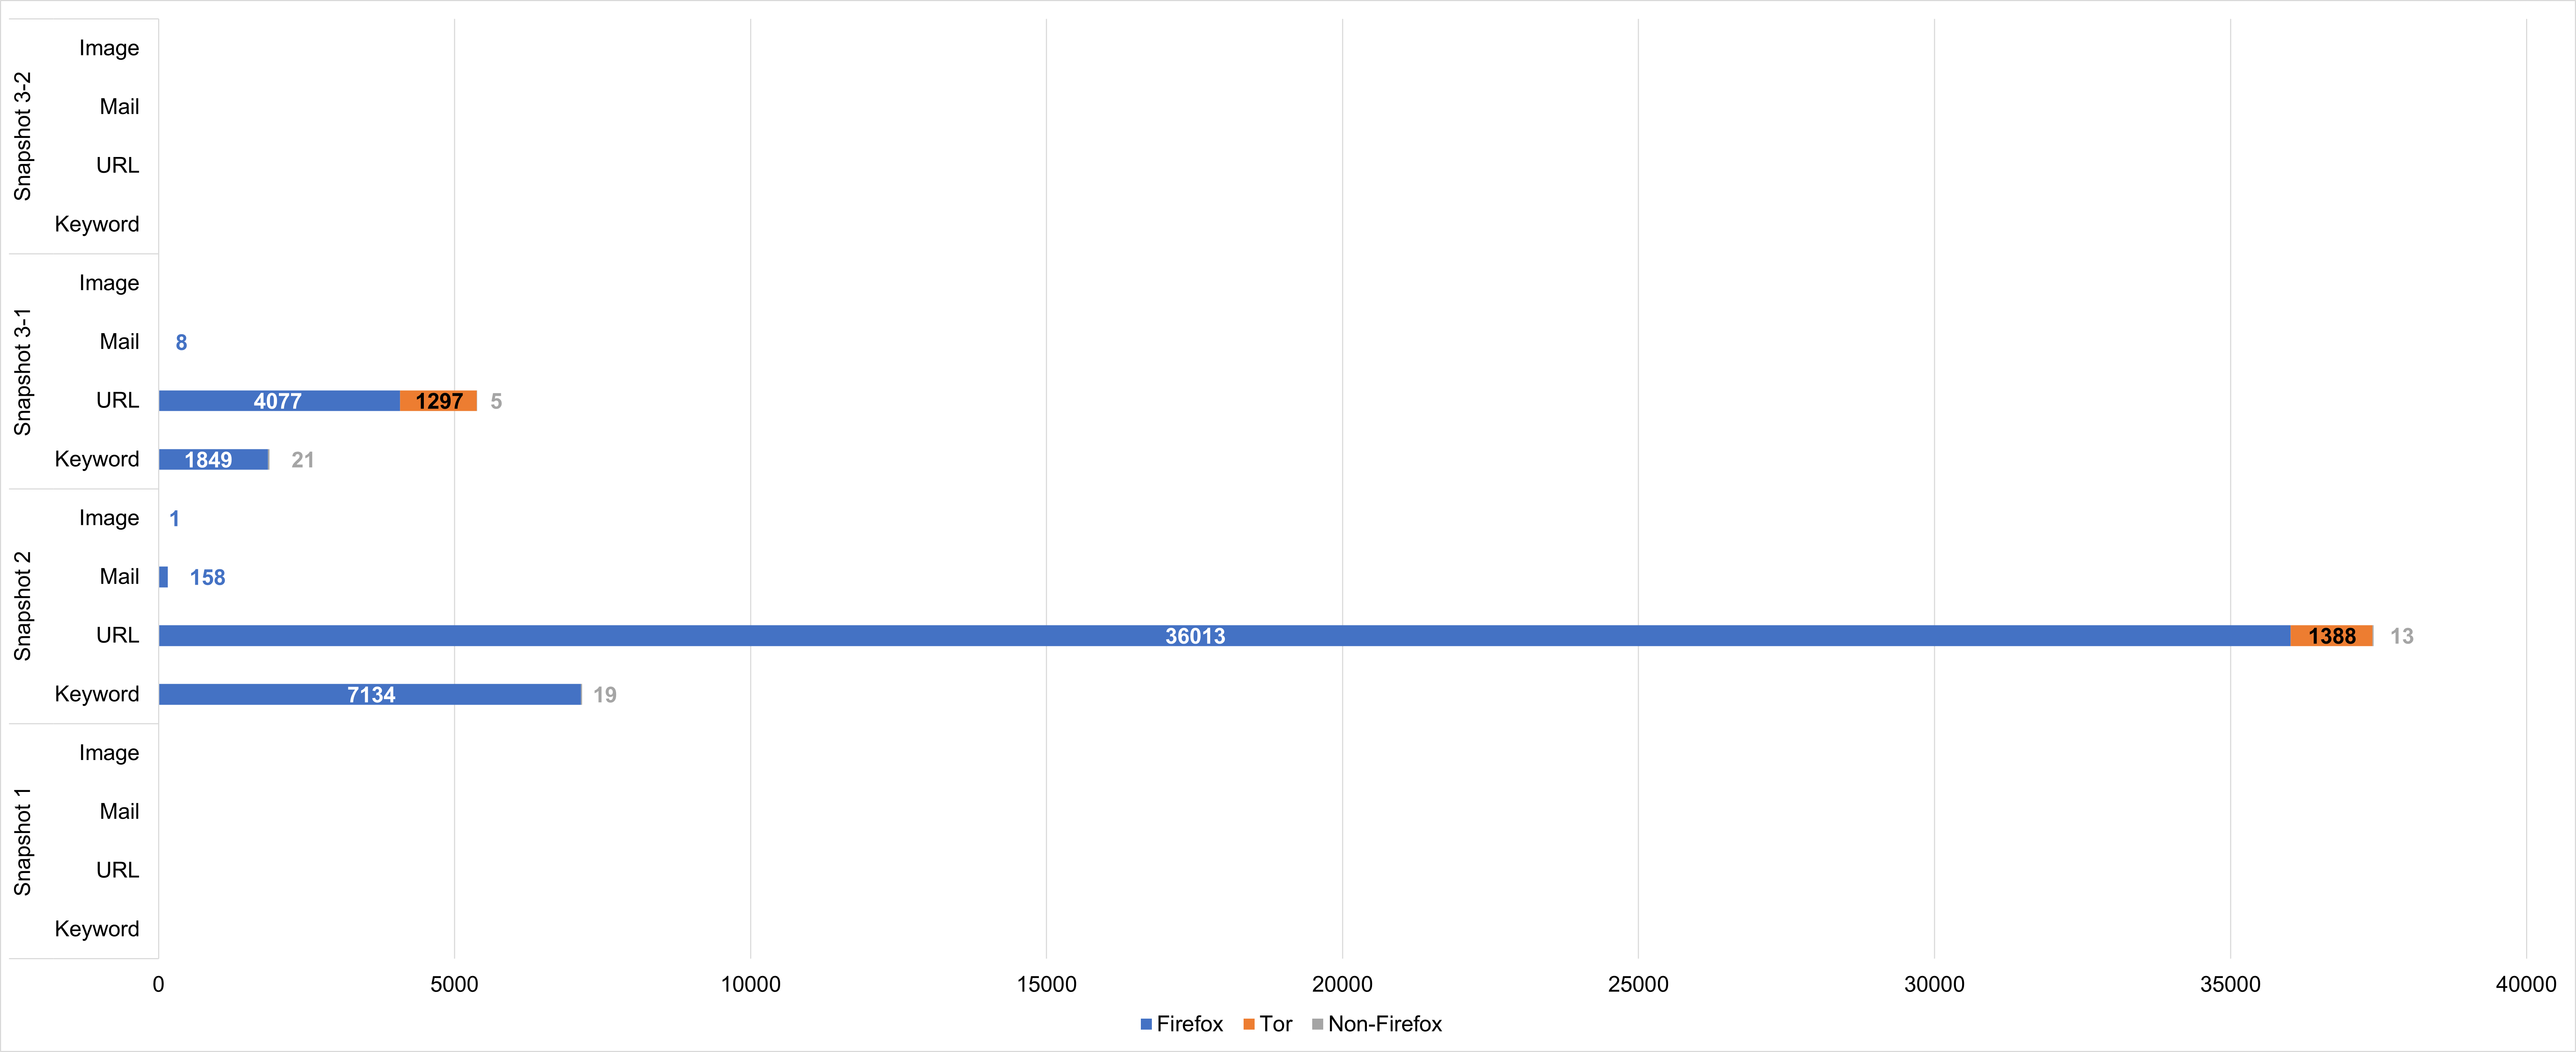
\includegraphics{bilder/volatility/tor/summary.png}}}
	\label{chart:final-criteria}  
	\caption{Summary}
\end{figure}
- PB Artefakte ausschließlich in RAM Dump 2 und 3-1 gefunden
- Nach Identitäts-Reset deutlich weniger Artefakte in vorhanden
- Am meisten URL-Artefakte gefunden, wobei mallofamerica.com dominant 
- HTML Artefakte wurden in keinem RAM Dump gefunden


TODO: Kreisdiagramme/Balkendiagramme mit Gesamtzahl an (Non-)Firefox Yarascan-Treffer erst im Vergleich mit Tor

\subsection*{Uncommon Locations}

Literatur:
%o Autopsy: \cite{Muir.2019}
%	•	Configuration files, downloaded files, and browserrelated data are recoverable from the file system.
%	•	Significant data-leakage from the browsing session occurred: HTTP header information, titles of web pages and an instance of a URL were found in registry files, system files, and unallocated space.
%o RAM-Analyse nach \cite{Muir.2019}:
%	•	Live-Analyse identifiziert auch nach dem Schließen und Deinstallieren des Browsers und Abmelden des Benutzers Spuren von Tor-Prozessen, einschließlich des absoluten Pfads zur Browser-Executable, des Benutzernamens und des Geräts, von dem es ausgeführt wurde.
%	•	The data-leakage contained the German word for ’search’ in reference to a Google search. This hints at the locale of the Tor server used to exit the network (exit relay).
%
%o RAM-Analyse nach \cite{Hariharan.2022}:
%	o	process was found to be firefox.exe
%	o	pslist and pstree: parent process was shown 
%	o	Belkasoft Ram Capturer: retrieve information about facebook
%	o	Cmdline: file path of the browser “E:/TorBrowser/Browser/firefox.exe” + name of process tor.exe and firefox.exe
%	o	Dlllist: DLL files of the executable files were not captured
%	o	Netscan: tor.exe + obfs4proxy.exe -> showed “LISTENING” connections to nonstandardized ports as output.
%	Yarascan: was able to retrieve all the browsing sessions
%o RAM-Analyse nach \cite{Sajan.2021} mit Volatility
%	•	process list extracted from the memory
%	•	registry hives been extracted from the memory dump
%	•	threads were extracted: “D:/VolatilityWorkbench/volatility.exe”–plugins=”D:/VolatilityWorkbench/profiles” pslistfilename =”C:/Users/username/Desktop/tor.raw” –profile=Win10x64 17763 –kdbg=0xf807606ac5e0
%	•	Handles: resources used by the process 5672
%	•	Dlls: These dlls can be found from prefetch file --> Can be found in “prefetch” file -> Analyzed with “winprefetchview”
%	•	Places.sqlite: SQLite viewer has been used to recover bookmarks and frequently visited sites even after uninstalling the application
%	•	Visited Websites: Using keyword search in Dump’s Hex
%
%o Registry:
%	> Shellactivites (siehe Firefox) \cite{Muir.2019}: instance of a URL were found in registry file
%	> \cite{Nelson.2020} The userassist key is located in the NTUSER.dat hive of the
%		 -> Registry and indicates the execution path of the program, as well as the number of times the program was executed 




\section{Chrome}

\subsection*{Uncommon Locations}

o Autopsy Keyword-Suche: 
	> Chrome and Edge produced five artefacts as reported by both tools. (FTK, Autopsy) \cite{Gabet.2018}
		--> Artefakte werden nicht genannt!
	> only two temporary files (Figure 7) were recovered with Minitool Power Data Recovery but it was a dead end; Location: appdata/…/Chrome/…/ Preferences/RF1533fa.TMP \cite{Fayyad.2021}
	> pagefile.sys file showed no traces at all \cite{Said.2011}
	

\section{Brave}
	
	\chapter{Vergleich der Browser}
\label{chapter:vergleich-der-browser}

In diesem Kapitel werden die untersuchten Browser hinsichtlich ihrer hinterlassenen PB-Artefakte verglichen.

\subsection*{Common Locations}
Bei keinem Browser konnten PB-Artefakte über die Analyse der Datei-Schreiboperationen in den Process Monitor Logfiles gefunden werden.
Ebenso konnten durch die genaue Untersuchung der Entwicklung der SQLite-Datenbanken aller Browser keine PB-Artefakte identifiziert werden.
Somit sind die Common Locations aller Browser während der gesamten Versuchsdurchführung frei von PB-Artefakten.

\subsection*{Registry}
Bei Betrachtung der Registry als Common Locations wurden keine PB-Artefakte in den Registry-Key bzw. -Values der Registry-Schreiboperationen der Process Monitor Logfiles gefunden.
Unter Betrachtung der Registry als Uncommon Locations konnten weder in System- noch User-Hives PB-Artefakte gefunden werden.
Somit befinden sich bei jedem Browser auch in der Registry zu keinem Zeitpunkt PB-Artefakte.

\subsection*{Uncommon Locations}
Weder über Autopsy Stichwortsuche noch in den automatisch von Autopsy kategorisierten Dateien konnten keine PB-Artefakte identifiziert werden.
%evtl. unterschiedlich Kategorisierte Dateien hervorheben

Einzig über die Untersuchung der Arbeitsspeicherabbilder mit Volatility konnten PB-Artefakte zu unterschiedlichen Zeitpunkten der Versuchsdurchführung identifiziert werden. 
Wie in Abbildung \ref{chart:all-browsers-ram-summary} dargestellt, konnten in keinem der Browser vor Durchführung des Browsing-Szenarios (RAM-Dump 1) PB-Artefakte im Arbeitsspeicher gefunden werden.
\begin{table}[h!]
	\resizebox{\linewidth}{!}{
	\begin{tabular}{r}
		\begin{tikzpicture}
			\begin{axis}[
			xbar,
			width=12cm, 
			height=3cm, 
			ylabel style={align=center}, ylabel=\textbf{RAM-Dump 1},
			y=1cm,
%			symbolic y coords={Suchbegriffe, URLs, E-Mail, DK-Logo},
			ytick = {1,...,5},
			yticklabels={Suchbegriffe, URLs, E-Mail, DK-Logo, HTML},
%			ytick=data,
			xticklabels={,,},
            xmin = 0,
            xmax = 42000,
			nodes near coords, 
			nodes near coords align={horizontal},
			nodes near coords style={font=\tiny},
   			nodes near coords={\pgfmathfloatifflags{\pgfplotspointmeta}{0}{}{\pgfmathprintnumber{\pgfplotspointmeta}}},
			bar width=.2cm,
			enlarge y limits={abs=2*\pgfplotbarwidth},
			scaled x ticks=false,
    		yminorgrids = true,minor tick num=1,
			legend style={
				at={(0.5,-0.1)},
				anchor=north
			},
			legend columns=4
			]
				\addplot coordinates {
				(0,1) (0,2) (0,3) (0,4) (0,5)
				};
				\addplot coordinates {
				(0,1) (0,2) (0,3) (0,4) (0,5)
				};
				\addplot coordinates {
				(0,1) (0,2) (0,3) (0,4) (0,5)
				};
				\addplot coordinates {
				(0,1) (0,2) (0,3) (0,4) (0,5)
				};
%			\legend{Firefox, Tor, Chrome, Brave}
			\end{axis}
		\end{tikzpicture}	
		\\[-7pt]
		\begin{tikzpicture}
			\begin{axis}[
			xbar,
			width=12cm, 
			height=3cm, 
			ylabel style={align=center}, ylabel=\textbf{RAM-Dump 2},
			y=1.2cm,
%			symbolic y coords={Suchbegriffe, URLs, E-Mail, DK-Logo},
			ytick = {1,...,5},
			yticklabels={Suchbegriffe, URLs, E-Mail, DK-Logo, HTML},
			ytick=data,
			xticklabels={,,},
            xmin = 0,
            xmax = 42000,
			nodes near coords, 
			nodes near coords align={horizontal},
			nodes near coords style={font=\tiny},
   			nodes near coords={\pgfmathfloatifflags{\pgfplotspointmeta}{0}{}{\pgfmathprintnumber{\pgfplotspointmeta}}},
			bar width=.2cm,
			enlarge y limits={abs=3*\pgfplotbarwidth},
			scaled x ticks=false,
    		yminorgrids = true,minor tick num=1,
			legend style={
				at={(0.5,-0.1)},
				anchor=north
			},
			legend columns=4
			]
				\path  [red,line width=0pt] (axis cs: 500,3.977) -- (axis cs: 500,3.8)
				node[pos = 0.5,right] {\tiny,$\,$*0};
				\addplot coordinates {
				(1983,1) (8655,2) (184,3) (3,4) (0,5)
				};
				\path  [red,line width=0pt] (axis cs: 1550,2.977) -- (axis cs: 1550,2.8)
				node[pos = 0.5,right] {\tiny,$\,$*8};
				\addplot coordinates {
				(7163,1) (37414,2) (158,3) (1,4) (0,5)
				};
				\draw [red,line width=0.5pt] (axis cs: 5379,1.977) -- (axis cs: 5379,1.8)
				node[pos = 0.5,right] {\tiny*5,379};
				\addplot coordinates {
				(3301,1) (17048,2) (590,3) (3,4) (1,5)
				};
				\draw [red,line width=0.5pt] (axis cs: 1870,0.977) -- (axis cs: 1870,0.8)
				node[pos = 0.5,right] {\tiny*1,870};
				\addplot coordinates {
				(2124,1) (10132,2) (408,3) (3,4) (1,5)
				};
			\end{axis}
%			\legend{Firefox, Tor, Chrome, Brave}
		\end{tikzpicture}
		\\[-7pt]
		\begin{tikzpicture}
			\begin{axis}[
			xbar,
			width=12cm, 
			height=3cm, 
			ylabel style={align=center}, ylabel=\textbf{RAM-Dump 3},
			y=1.2cm,
			symbolic y coords={Suchbegriffe, URLs, E-Mail, DK-Logo, HTML},
			ytick=data,
			xticklabels={,,},
            xmin = 0,
            xmax = 42000,
			nodes near coords, 
			nodes near coords align={horizontal},
			nodes near coords style={font=\tiny},
   			nodes near coords={\pgfmathfloatifflags{\pgfplotspointmeta}{0}{}{\pgfmathprintnumber{\pgfplotspointmeta}}},
			bar width=.2cm,
			enlarge y limits={abs=2*\pgfplotbarwidth},
			scaled x ticks=false,
    		yminorgrids = true,minor tick num=1,
			legend style={
				at={(0.5,-0.1)},
				anchor=north
			},
			legend columns=4
			]
				\addplot coordinates {
				(0,Suchbegriffe) (91,URLs) (0,E-Mail) (0,DK-Logo) (0,HTML)
				};
				\addplot coordinates {
				(0,Suchbegriffe) (0,URLs) (0,E-Mail) (0,DK-Logo) (0,HTML)
				};
				\addplot coordinates {
				(0,Suchbegriffe) (5,URLs) (1,E-Mail) (0,DK-Logo) (0,HTML)
				};
				\addplot coordinates {
				(0,Suchbegriffe) (0,URLs) (1,E-Mail) (0,DK-Logo) (0,HTML)
				};
				\legend{Firefox, Tor, Chrome, Brave}
			\end{axis}
		\end{tikzpicture}
	\end{tabular}
	}
	\captionof{figure}{Zusammenfassung gefundener Artefakte im RAM der Browser}
	\label{chart:all-browsers-ram-summary}
\end{table}

\paragraph*{Firefox vs Tor}
%> RAM-Dump 2: 
Tor hinterlässt nach dem Browsing-Szenario, vor Zuweisung einer \grqq{}Neuen Identität\grqq{} mehr URL-Artefake und Suchbegriffe im RAM als Firefox (RAM-Dump 2). 
Sowohl bei Tor als auch bei Firefox ist zu diesem Zeitpunkt das Gmail-Passwort als Klartext im RAM identifizierbar.
Wie anhand der roten, mit * gekennzeichneten Werte in Abbildung \ref{chart:all-browsers-ram-summary} zu erkennen ist, 
reduzieren sich die hinterlassenen Artefakte nach Zuweisung einer \grqq{}Neuen Identität\grqq{} beim Tor-Browser deutlich, sodass danach weniger Artefakte als bei Firefox vorhanden sind.
Wie in Abschnitt \ref{section:methodik-vorbereitung-browserauswahl} erklärt, ermöglicht die \grqq{}Neue Identität\grqq{} das Schließen von Tabs und Fenstern, das Löschen von privaten Informationen und die Neukonfiguration der Tor-Netzwerkverbindung.
Mit der \grqq{}Neuen Identität\grqq{} ist bei Tor das Passwort nicht mehr als Klartext im Arbeitsspeicher zu identifizieren.
%> RAM-Dump 3:
Nach Schließen des Browsers (RAM-Dump 3) hinterlässt der Tor Browser keine Artefakte, bei Firefox konnten noch 91 URLs im DNSCache gefunden werden. 
Keiner der beiden Browser hinterließ zu irgendeinem Zeitpunkt HTML-Artefakte.
%Gewinner:
%> RAM-Dump 2:
%	- Vor \grqq{}Neue Identität\grqq{}: Firefox
%	- Nach \grqq{}Neuer Identität\grqq{}: Tor 
%> RAM-Dump 3:
%	- Tor 
%Somit hinterlässt Tor sowohl nach dem Browsing-Szenario mit \grqq{}Neuer Identität\grqq{} als auch mit geschlossenem Browser weniger PB-Artefakte als Firefox.

\paragraph*{Chrome vs Brave}
Chrome und Brave hinterlassen jeweils nur im zweiten und dritten RAM-Dump PB-Artefakte. Beide Browser hinterlassen in zweiten RAM-Dump gleich viele Artefakte in den Kategorien HTML (eins), DK-Logo (drei) sowie im dritten RAM-Dump in der Kategorie E-Mail (eins). Bei den Kategorien E-Mail, URLs sowie bei den Suchbegriffen hinterließ Brave dabei jeweils weniger Artefakte als der Browser Chrome. Bei keinem der beiden Browser konnte zu irgendeinem Zeitpunkt ein Passwort-Artefakt im RAM festgestellt werden.

\paragraph*{Firefox vs Chrome}
%> In RAM-Dump 2: 
Firefox hinterlässt nach dem Browsing-Szenario mit geöffnetem Browser (RAM-Dump 2) in jeder Kategorie gleich viele (DK-Logo) oder weniger (E-Mail, URLs, Suchbegriffe, HTML) Artefakte als Chrome.
Dabei werden bei Firefox im zweiten RAM-Dump durchschnittlich 2.024 Artefakte weniger gefunden als bei Chrome.
%> In Ram-Dump 3: 
Nach Schließen des Browsers (RAM Dump 3) hinterlässt Firefox mehr URLs im Arbeitsspeicher als Chrome. Im RAM-Dump von Chrome wurde zusätzlich die Absender-Adresse gefunden.
%Gewinner:
%RAM-Dump 2:
%	- Firefox
%RAM-Dump 3: 
%	- URLs: Chrome
%	- E-Mail: Firefox

\paragraph*{Tor vs Brave}
Vor Zuweisung der \grqq{}Neuen Identität\grqq{} hinterlässt der Tor-Browser nach dem Browsing-Szenario  deutlich mehr URL- und Suchbegriff-Artefakte als Brave (RAM-Dump 2). Insbesondere hinterlässt Tor zweimal das Passwort des Google-Accounts als Klartext im RAM.
Nach Zuweisung der \grqq{}Neuen Identität\grqq{} des Tor-Browsers hinterlässt dieser durchschnittlich 1315 Artefakte weniger als Brave.
Nach Schließen des Browsers (RAM-Dump 3) hinterlässt Tor kein Artefakt im RAM, Brave einmal die Absender-Mail. 
%Gewinner:
%RAM-Dump 2:
%	- DK-Logo, E-Mail: Tor
%	- URLs, Suchbegriffe: Brave (Vor \grqq{}Neue Identität\grqq{}), Tor (Nach \grqq{}Neuer Identität\grqq{}) 
%RAM-Dump 3: Tor

\paragraph*{Quantitativer Vergleich aller Browser}
Um unter den vier untersuchten Browsern denjenigen mit den wenigsten PB-Artefakten zu ermitteln, wird eine in Tabelle \ref{tab:gewinner-tabelle} gezeigte, sogenannte  \textit{Gewinner-Tabelle} erstellt \cite{Horsman.2019}.

\begin{table}[h!]
	\caption{Gewinner-Tabelle der vier untersuchten Browser}
	\label{tab:gewinner-tabelle}
	\centering
	\resizebox{\linewidth}{!}{
	\begin{tabular}{c|c|c|c|c|c|c}
	\cline{2-7}
	\multicolumn{1}{l|}{}                                                                                                & \textbf{Suchbegriffe}                   & \textbf{URLs}                                                                                     & \textbf{E-Mail}                                                                                    & \textbf{DK-Logo}                    & \textbf{HTML}                                                                           & \multicolumn{1}{c|}{\textbf{\begin{tabular}[c]{@{}c@{}}Gewinner \\ pro RAM-Dump\end{tabular}}} \\ \hline
	\multicolumn{1}{|c|}{\textbf{RAM-Dump 1}}                                                                            & Unentschieden                           & Unentschieden                                                                                     & Unentschieden                                                                                      & Unentschieden                       & Unentschieden                                                                           & \multicolumn{1}{c|}{{\color[HTML]{FE0000} \textbf{Unentschieden}}}                             \\ \hline
	\multicolumn{1}{|c|}{\textbf{\begin{tabular}[c]{@{}c@{}}RAM-Dump 2\\ (ohne "Neuer ID")\end{tabular}}}                & Firefox                                 & Firefox                                                                                           & Brave*                                                                                             & Tor                                 & \begin{tabular}[c]{@{}c@{}}Firefox, \\ Tor\end{tabular}                                 & \multicolumn{1}{c|}{{\color[HTML]{FE0000} \textbf{Firefox}}}                                   \\ \hline
	\multicolumn{1}{|c|}{\textbf{\begin{tabular}[c]{@{}c@{}}RAM-Dump 2\\ (mit "Neuer ID")\end{tabular}}}                 & Tor                                     & Tor                                                                                               & Tor                                                                                                & Tor                                 & \begin{tabular}[c]{@{}c@{}}Firefox, \\ Tor\end{tabular}                                 & \multicolumn{1}{c|}{{\color[HTML]{FE0000} \textbf{Tor}}}                                       \\ \hline
	\multicolumn{1}{|c|}{\textbf{RAM-Dump 3}}                                                                            & Unentschieden                           & Tor, Brave                                                                                        & \begin{tabular}[c]{@{}c@{}}Firefox, \\ Tor\end{tabular}                                            & Unentschieden                       & Unentschieden                                                                           & \multicolumn{1}{c|}{{\color[HTML]{FE0000} \textbf{Tor}}}                                       \\ \hline
	\multicolumn{1}{|c|}{\textbf{\begin{tabular}[c]{@{}c@{}}Gewinner pro \\ Kategorie\\ (ohne "Neuer ID")\end{tabular}}} & {\color[HTML]{FE0000} \textbf{Firefox}} & {\color[HTML]{FE0000} \textbf{\begin{tabular}[c]{@{}c@{}}Firefox, \\ Tor, \\ Brave\end{tabular}}} & {\color[HTML]{FE0000} \textbf{\begin{tabular}[c]{@{}c@{}}Firefox, \\ Tor, \\ Brave*\end{tabular}}} & {\color[HTML]{FE0000} \textbf{Tor}} & {\color[HTML]{FE0000} \textbf{\begin{tabular}[c]{@{}c@{}}Firefox, \\ Tor\end{tabular}}} & \multicolumn{1}{l}{}                                                                           \\ \cline{1-6}
	\multicolumn{1}{|c|}{\textbf{\begin{tabular}[c]{@{}c@{}}Gewinner pro \\ Kategorie\\ (mit "Neuer ID")\end{tabular}}}  & {\color[HTML]{FE0000} \textbf{Tor}}     & {\color[HTML]{FE0000} \textbf{Tor}}                                                               & {\color[HTML]{FE0000} \textbf{Tor}}                                                                & {\color[HTML]{FE0000} \textbf{Tor}} & {\color[HTML]{FE0000} \textbf{\begin{tabular}[c]{@{}c@{}}Firefox, \\ Tor\end{tabular}}} & \multicolumn{1}{l}{}                                                                           \\ \cline{1-6}
	\end{tabular}
	}
\end{table}
\begin{sloppypar}
Dabei liegt der Fokus auf den Kategorien der PB-Artefakte:  Es wird für jede RAM-Dump/Kategorie Kombination derjenige Browser mit den wenigsten PB-Artefakten ermittelt. 
Somit wird die Anzahl gefundener Artefakte nur innerhalb einer Kategorie verglichen. Die Differenz gefundener PB-Artefakte wird dabei nicht berücksichtigt.\end{sloppypar}
Daraus ergeben sich zwei Arten von \textit{Gewinnern}:
\begin{itemize}
\item \textbf{Gewinner pro RAM-Dump}: Browser, der innerhalb eines RAM-Dumps am häufigsten die wenigsten PB-Artefakte einer Kategorie hinterlässt. (Zeilenweiser Mehrheitsentscheid)
\item \textbf{Gewinner pro Kategorie}: Browser, der innerhalb einer Kategorie am häufigsten die wenigsten PB-Artefakte in den RAM-Dumps hinterlässt. (Spaltenweiser Mehrheitsentscheid)
\end{itemize}

Um ein differenziertes Ergebnis zu ermitteln, wird bei RAM-Dump 2 zusätzlich unterschieden, ob der Tor-Browser vor- oder nach der Zuweisung der \grqq{}Neuen Identität\grqq{}, kurz \grqq{}Neue ID\grqq{}, bewertet wird. 
Diese Unterscheidung findet ebenfalls bei den Gewinnern statt. Die in Tabelle \ref{tab:gewinner} ermittelten vier Gewinner ergeben sich per Mehrheitsentscheid innerhalb der jeweiligen Gewinner-Kategorie. 

\begin{table}[h!]
	\centering
	\caption{Ermittelte Gewinner gemäß Gewinner-Tabelle}
	\label{tab:gewinner}
	\resizebox{0.8\linewidth}{!}{
	\begin{tabular}{c|c|c|}
	\cline{2-3}
	\multicolumn{1}{l|}{}                                 & \textbf{Mit \grqq{}Neuer Identität\grqq{}} & \textbf{Ohne \grqq{}Neuer Identität\grqq{}} \\ \hline
	\multicolumn{1}{|c|}{\textbf{Gewinner pro RAM-Dump}}  & Tor                            & Firefox, Tor                    \\ \hline
	\multicolumn{1}{|c|}{\textbf{Gewinner pro Kategorie}} & Tor                            & Firefox, Tor                    \\ \hline
	\end{tabular}
	}
\end{table}

Unter Berücksichtigung der \grqq{}Neuen Identität\grqq{} ist der Tor-Browser sowohl der Gewinner pro RAM-Dump als auch pro Kategorie.
Ohne Berücksichtigung ist neben dem Tor-Browser auch Firefox Gewinner pro RAM-Dump und pro Kategorie. Somit ist gemäß Auswertung der Gewinner-Tabelle der Tor-Browser derjenige Browser mit den wenigsten PB-Artefakten, gefolgt von Mozilla Firefox.












	
	\chapter{Zusammenfassung und Diskussion}\label{chap:Zusammenfassung-Diskussion}

\begin{comment}

> Artefakte im DNS Cache: \cite{Satvat.2014}
	•	DNS-Caching ist eine Bedrohung für private Browsing
	•	Diese Schwachstelle entsteht, weil das Betriebssystem DNS-Anfragen des Browsers im Cache speichert, unabhängig davon, ob der Browser im privaten Modus ist oder nicht
	•	Mehrere Jahre nach der Meldung dieser Schwachstelle besteht sie immer noch in allen Browsern fort
	•	Es wurden einige Erweiterungen von Drittanbietern entwickelt, um dieses Problem zu beheben, aber keine davon wurde von den Browserherstellern übernommen.
	


> Viele RAM-Artefakte
	- Firefox \cite{Muir.2019}
		•	Darcie et al. (2014) fanden Beweise für das Web-Browsing in Form von JPEG- und HTML-Dateien in Live-Forensik, aber eine statische Forensik war erfolglos.
		•	Eine vorherige Live-Forensik-Analyse des Firefox-Browsers zeigte, dass Artefakte aus einer privaten Browsing-Sitzung aus dem Speicher wiederhergestellt werden konnten. (Findlay and Leimich, 2014). 
		

> IE hinterlässt viele Spuren im Gegensatz zu Ergebnissen: \cite{Md.2018}
	o	hidden folders are usually stored at C/Users/User/AppData
	o	evidence searches are conducted extensively in the C:\ partition
	o	bookmarks remain and can be viewed
	o	downloads remain in the downloads folder until the user manually deletes them
	o	CacheView trace entire URL and browsing histories including the temporary files
	CacheView enables to find the image’s URL and from specific website
	
> Urteil über die Privatheit von Tor nach \cite{Muir.2019}
	The design aim of preventing Tor from writing to disk (Perry et al., 2018) is not achieved in this version.
		•	Configuration files, downloaded files, and browserrelated data are recoverable from the file system.
		•	Significant data-leakage from the browsing session occurred: HTTP header information, titles of web pages and an instance of a URL were found in registry files, system files, and unallocated space.
		•	The data-leakage contained the German word for ’search’ in reference to a Google search. This hints at the locale of the Tor server used to exit the network (exit relay).
	The Tor Project’s design aim of enabling secure deletion of the browser (Sandvik, 2013) is not achieved in this version.
		•	References to: the installation directory, Firefox SQLite files, bridging IPs/ports, default bookmarks, Tor-related DLLs and Tor product information were all recovered after the browser was deleted.
		•	In a scenario where the operating system paged memory, an instance

Weiterführende Arbeiten:
> Cross-mode interference \cite{Hedberg.2013}:
	o	the Chrome://memory page displays all the opened tabs in the browser regardless if they are in the usual or private mode -> Nicht mehr aktuell -> Stattdessen: Chrome Task-manager (Ctrl + Esc), Funktioniert auch bei Firefox
> Unser Scope: Process Monitor nach Prozessnamen gefiltert
	- Weiterführend: Nach Pathnamen filtern: "Common Locations"

> Für wen wird Browser entwickelt
> Warum und für wen wird Private Browsing analysiert?
> Ist das Auffinden privater Browsing Artefakte Schuld von Browser Entwicklern? (Oder Schuld des Betriebssystem, wie in (TODO!) erwähnt)
\end{comment}


Zusammenfassend liefern alle der vier betrachteten Browser ein gutes Ergebnis, da keine Browsing-Artefakte im nichtvolatilen, also persistenten Speicher identifiziert werden konnten. Jene konnten nur im RAM gefunden werden und teilweise im DNS-Cache, wobei diese auch durch das Leeren des Caches erfolgreich beseitigt worden konnten. Artefakte im DNS-Cache sind dabei eine bekannte Problematik. DNS-Anfragen des Browsers werden dabei von Betriebssystem darin gespeichert, unabhängig davon, ob der Browser im privaten Modus ist oder nicht \cite{Satvat.2014}. Trotz der Bekanntheit dieser Schwachstelle besteht dieser immer noch in allen Browsern fort. Es wurden gezielt dafür auch schon Erweiterungen von Drittanbietern entwickelt, um dieses Problem des Speicherns von DNS-Anfragen zu cachen, jedoch wurde keine davon von den Browserherstellern übernommen \cite{Satvat.2014}. 

Wie in [link kap 6] übersichtlich dargelegt wurde, ist quantitativ gesehen der Tor-Browser der beste Browser, um am wenigsten Artefakte auf einem Computer zu hinterlassen. Zusätzlich zum Schutz vor einem local attacker bietet Tor den Vorteil, dass man dadurch auch noch vor web attackern geschützt ist, da der Datenverkehr über mehrere Router, den sogenannten Nodes, umleitet und somit die Herkunft der Anfrage verschleiert. Somit ist Tor als Gesamtpaket gesehen ein sicherer und guter Browser, um sicher und anonym im Internet zu browsen. \\
Trotz der gerade angesprochenen Vorteile muss man jedoch auch die Nachteile von Tor sehen. Erstens ist das Browsen an sich meistens langsamer, da der Datenverkehr eben über mehrere Knoten geleitet wird. Zusätzlich wird dabei der Internetverkehr auch noch verschlüsselt. Beides ist positiv für die Privatsphäre, schränkt aber die User Experience ein [cite webpage]. Zusätzlich dazu kann es dazu kommen, dass Websiten den Datenverkehr von Tor-Benutzern als potenzielles Sicherheitsrisiko ansehen und somit zusätzliche Captchas und Sicherheitsmaßnahmen einfügen, was wieder die User Experience einschränkt. Dazu kommt auch noch, dass man von der Infrastruktur des Tor-Netzwerkes angewiesen ist und es zu Verbindungsproblemen führen kann, wenn das Netzwerk gestört ist oder bestimmte nodes nicht verfügbar sind. \\
Hier muss jedoch beachtet werden, dass Tor in dieser Arbeit nur quantitativ gesehen der beste Browser ist, da er die wenigsten Artefakte von allen analysierten Browsern hinterlässt. Qualitativ gesehen kann es jedoch für einen Benutzer wichtiger sein, dass ein Browser ein Passwort nicht im RAM ablegt und somit davon keine Spuren  auf dem System hinterlässt. Somit kann die objektive Auffassung, dass Tor aufgrund der wenigen Artefakte der beste Browser ist, subjektiv gesehen auch für jemand anderen ein schlechterer Browser sein, wenn beispielsweise das Auffinden von HTML-Artefakten ein weniger kritisches Verhalten darstellt. In diesem Fall wären dann die beiden Browser Chrome und Brave \glqq{}besser\grqq{} bzw. \glqq{}sicherer\grqq{}.

\thispagestyle{plain.scrheadings}
\ohead{}
Schließlich ist noch die Frage zu klären, für welche Personen diese Analyse grundsätzlich durchgeführt wird bzw. wer von solch einer forensischen Analyse einen Nutzen zieht. Grundsätzlich wird eine solche forensische Analyse durchgeführt, um Schwächen in Browsern und den privaten Modi aufzudecken. Von diesen Ergebnissen profitieren zunächst einmal die Browser-Entwickler, welche auf Basis der Ergebnisse das Ziel haben (sollten), die aufgedeckten Schwächen zu beseitigen, um ein privateres und sichereres Browsen zu ermöglichen. Dieses private Browsen kann dann entweder genutzt werden, um von „normalen“ Benutzern für legale Aktivitäten verwendet zu werden, oder von Kriminellen für illegale Tätigkeiten. Für diese wäre es dann sinnvoll, wenn der Browser möglichst wenige Artefakte verursacht, um möglichst unerkannt diesen Tätigkeiten nachzugehen. Dies würde es jedoch Forensikern wieder schwieriger machen, jene Tätigkeiten aufzudecken und nachzuweisen. Auch profitieren von solchen Analysen die Forensiker, welche auf Basis der Ergebnisse gezielt nach Artefakten suchen können und es somit leichter gemacht wird, kriminelle Tätigkeiten aufzudecken. \\
Wie daraus ersichtlich wird, ist es nicht einfach zu sagen, wem eine solche forensische Analyse zunächst mehr nutzt und ob es gut oder schlecht ist, eine solche zu betreiben, da man nicht vorhersagen kann, ob die Ergebnisse zuerst gutartig zum besseren Aufdecken von illegalen Aktivitäten oder bösartig zum besseren Verschleiern von diesen verwendet wird. Ebenfalls ist nicht sicher, ob eventuell bestehende Sicherheitslücken bestehen bleiben sollten, um das Aufdecken illegaler Aktivitäten zu erleichtern.


	
	\chapter{Fazit}

Einleitend werden Struktur, Motivation und die abgeleiteten Forschungsfragen diskutiert.
	
	%\renewcommand\thefigure{\thesection.\arabic{figure}}   
%\renewcommand\thetable{\thesection.\arabic{figure}}
\counterwithin{figure}{section}
\counterwithin{table}{section}

\begin{appendices}
	%	\addtocontents{lof}{\protect\contentsline{chapter}{%
			%			Appendices \vspace{10pt}
			%	}{}
%		\addtocontents{toc}{\protect\setcounter{tocdepth}{1}}
%		\makeatletter
%		\addtocontents{toc}{%
%			\begingroup
%			\let\protect\l@chapter\protect\l@section
%			\let\protect\l@section\protect\l@subsection
%		}
%		\makeatother
		
%		\huge{\textbf{All File Operations Firefox}}
%%		\enlargethispage{6cm}

%		
%		\huge{\textbf{All File Operations Tor}}
%%		\enlargethispage{6cm}
%		\begin{figure}[h!]
%			\centerline{\resizebox{!}{0.9\textheight}{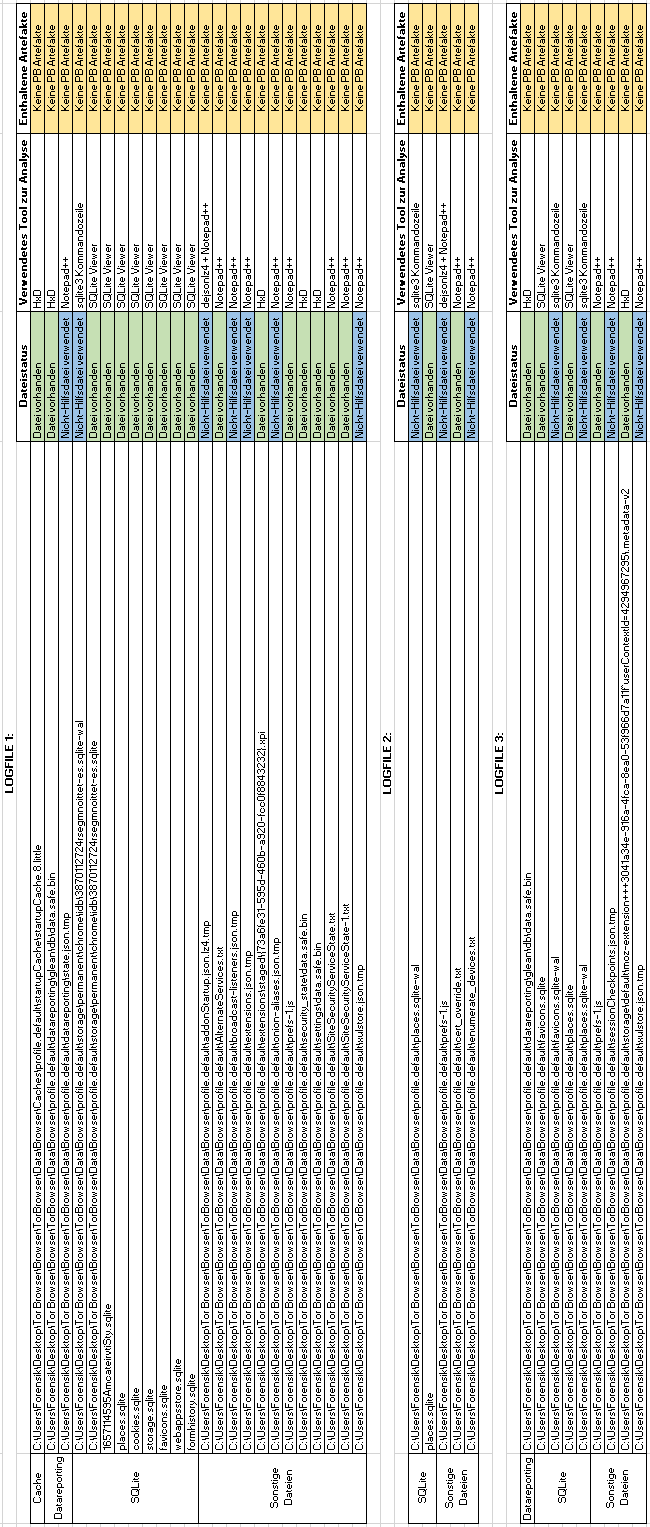
\includegraphics{bilder/tor-all-write-operations.png}}}
%			%	\label{...}
%			\caption{All File Operations Firefox: Logfile 1 vs. Logfile 2 vs. Logfile 3}
%		\end{figure}

\renewcommand{\thesection}{\Alph{section}}

\newgeometry{left=1.5cm,bottom=2cm,top=0.5cm}
\begin{landscape}% Landscape page
	\section{Yara-Regeln}
	\label{appendix:yara-regeln}
	%\setcounter{page}{43}
%	\thispagestyle{empty}
	\vspace*{-0.5cm}
%	\hspace*{-1cm}
%\begin{table}

\begin{multicols}{2}
		\begin{minted}[
			obeytabs=true,
			tabsize=2,
			autogobble,
			fontsize=\footnotesize,
			frame=single
			]{text}
			rule keyword {
				strings:
					$pfaffenhofen_keyword="pfaffenhofen" wide ascii nocase
					$nanoradar_keyword="nanoradar" wide ascii nocase	
				condition:
					$pfaffenhofen_keyword or $nanoradar_keyword 
			}
			
			rule keyword_mooserliesl {
				strings:
					$mooserliesl1_keyword="mooserliesl" wide ascii nocase
					$mooserliesl1_keyword2="mooserliesl.de" wide ascii nocase	
				condition:
					$mooserliesl1_keyword and not $mooserliesl1_keyword2
			}
			
			rule keyword_mallofamerica {
				strings:		
					$mallofamerica1_keyword="mallofamerica" wide ascii nocase
					$mallofamerica1_keyword2="mallofamerica.com" wide ascii nocase	
				condition:
					$mallofamerica1_keyword and not $mallofamerica1_keyword2
			}
			
			rule url {
				strings:
					$mallofamerica_url="mallofamerica.com" wide ascii nocase
					$mooserliesl_url="mooserliesl.de" wide ascii nocase
					$unitree_url="unitree.com" wide ascii nocase
					$donaukurier_url="donaukurier.de" wide ascii nocase	
				condition:
					$mallofamerica_url or $mooserliesl_url or $unitree_url or $donaukurier_url
			}
			
			rule html {
				strings:			
					$mallofamerica_html="Insiders</span>" wide ascii nocase
					$mooserliesl_html="Ja</span>" wide ascii nocase
					$unitree_html="L1</div>" wide ascii nocase
					$donaukurier_html=">Themen:" wide ascii nocase		
				condition:
					$mallofamerica_html or $mooserliesl_html or $unitree_html
					or $donaukurier_html
			}
			
			rule image {
				strings:
					$image_hex = {
								  89 50 4E 47 0D 0A 1A 0A 00 00 00 0D 49 48 44 52 00 00 01 2C 00 00 
								  00 32 08 03 00 00 00 D1 08 16 18 00 00 00 19 74 45 58 74 53 6F 66 
								  74 77 61 72 65 00 41 64 6F 62 65 20 49 6D 61 67 65 52 65 61 64 79 
								  71 C9 65 3C 00 00 03 84 69 54 58 74 58 4D 4C 3A 63 6F 6D 2E 61 64 
								  6F 62 65 2E 78 6D 70 00 00 00 00 00 3C 3F 78 70 61 63 6B 65 74 20 
																 ...
								  4E AD 38 61 03 55 6A AB 5E BF F6 40 4E 9D BA 20 FE 43 FE 99 81 2C 
								  0A 8F B2 F1 D8 7B DE E5 75 7E 45 E3 FC E4 C8 81 E5 C0 72 60 39 B0 
								  1C 71 60 39 B0 1C 58 0E 2C 07 D6 FF A9 FC 57 80 01 00 D9 B2 CD 5E 
								  42 B8 37 25 00 00 00 00 49 45 4E 44 AE 42 60 82}
				condition:
					$image_hex
			}
			
			rule mail {
				strings:		
					$computerforensik_address="computerforensikvl@gmail.com" wide ascii nocase
					$computerforensik_password="Vorlesung23!" wide ascii nocase
					$cas0597_address="cas0597@thi.de" wide ascii nocase
					$chs3702_address="chs3702@thi.de" wide ascii nocase
					$subject="Betrefftext" wide ascii nocase
					$mail_body="Mailinhalt" wide ascii nocase	
				condition:
					$computerforensik_address or $computerforensik_password 
					or $cas0597_address or $chs3702_address or $subject 
					or $mail_body
			}
		\end{minted}
\end{multicols}

%\end{table}
%%	\vspace{-1cm}
%	\caption{Yara-Regeln}
%	\label{code:yara-rule}
\end{landscape}
\restoregeometry

\section{Ausführliche Analyse: Firefox}\label{section:appendix-firefox}
\subsection{Common Locations}
\label{subsection:appendix-firefox-common-locations}
\subsubsection*{Process Monitor WriteFile Operations}
\label{subsubsection:appendix-firefox-common-locations-writefile-operations}
Gemäß Versuchsdurchführung wurden für Firefox mit dem Process Monitor Tool zwei Logfiles erstellt. Diese Dateien enthalten alle aufgezeichneten Prozessaktivitäten während und nach dem Browsing-Szenario.
Zunächst wurden beide Logfiles gemäß Methodik in Kapitel \ref{subsection:methodik-datensammlung-processmonitorlogfiles} in Excel aufbereitet. Tabelle \ref{tab:firefox-writefile-operations} listet alle in den gefilterten Logfiles identifizierten Dateien auf. Dabei wurde für jede Datei vermerkt, ob und wie sie wiederherstellbar war, mit welchem Tool die Datei analysiert wurde und ob in der Datei PB-Artefakte enthalten sind. Die wiederherstellbaren Dateien wurden in die Kategorien \textit{Cache}, \textit{Datareporting}, \textit{Sessionstore-Backup} und \textit{Sonstige Dateien} eingeordnet. In keiner der Dateien wurden PB-Artefakte identifiziert.

Bei detaillierter Untersuchung der wiederherstellbaren Dateien konnten zwei Pfade identifiziert werden, in die Firefox während des Versuchs Dateien schreibt: 
\begin{itemize}
\item \textbf{Local:} \texttt{C:$\backslash$Users$\backslash$<User>$\backslash$AppData$\backslash$Local$\backslash$Mozilla$\backslash$Firefox$\backslash$Profiles$\backslash$\\<Profile>.default-release$\backslash$}
\item \textbf{Roaming:} \texttt{C:$\backslash$Users$\backslash$<User>$\backslash$AppData$\backslash$Roaming$\backslash$Mozilla$\backslash$Firefox$\backslash$Profiles$\backslash$\\<Profile>.default-release$\backslash$}
\end{itemize}
In Tabelle 	\ref{tab:firefox-writefile-operations} sind die Dateien je nach Speicherort \textit{Local} (Hellblau) oder \textit{Roaming} (Dunkelblau) entsprechend eingefärbt. Im Speicherort Local sind ausschließlich Dateien der Kategorie \grqq{}Cache\grqq{} gespeichert.

\paragraph*{Cache}
Firefox verwendet den Cache, um Webseiten und deren Ressourcen temporär lokal zu speichern. Dadurch können wiederholte Anfragen an den Server vermieden und die Ladezeiten verringert werden. Die Inhalte dieser Dateien sind binär.
Die Cache-Dateien im Format \texttt{$\backslash$cache2$\backslash$entries$\backslash$<ID>} werden im Local Pfad gespeichert.

%\newpage
\newgeometry{bottom=2cm,top=0.5cm}
%\setcounter{figure}{0}    
\afterpage{
\begin{landscape}% Landscape page
	\setcounter{page}{61}
%	\thispagestyle{empty}
	\vspace*{1.5cm}
	\hspace*{-1cm}
	\begin{table}[h!]
%	\centering
	\caption{Firefox alle \grqq{}WriteFile\grqq{}-Operationen der Logfiles 1 und 2}
	\label{tab:firefox-writefile-operations}
	\vspace{0.5cm}
	\resizebox{\linewidth}{!}{
	\begin{tabular}{cllll}
	\multicolumn{5}{c}{\textbf{LOGFILE 1:}}                                                                                                                                                                                                                                                                                                                                                                                                                                                                                                                     \\ \hline
	\multicolumn{1}{|c|}{\textbf{Kategorie}}                                                                     & \multicolumn{1}{c|}{\textbf{Dateiname}}                                                                                                                                                                             & \multicolumn{1}{c|}{\textbf{Dateistatus}}                                                         & \multicolumn{1}{c|}{\textbf{Tool für Analyse}}   & \multicolumn{1}{l|}{\textbf{Enthaltene Artefakte}}              \\ \hline
	\multicolumn{1}{|c|}{}                                                                                       & \multicolumn{1}{l|}{\cellcolor[HTML]{34CDF9}\textbackslash{}cache2\textbackslash{}entries\textbackslash{}037778A55E1B7E9BED3390289866D09402D6C913}                                                                  & \multicolumn{1}{l|}{\cellcolor[HTML]{009901}Datei vorhanden}                                      & \multicolumn{1}{l|}{MZCacheView}            & \multicolumn{1}{l|}{\cellcolor[HTML]{F8A102}Keine PB-Artefakte} \\ \cline{2-5} 
	\multicolumn{1}{|c|}{}                                                                                       & \multicolumn{1}{l|}{\cellcolor[HTML]{34CDF9}\textbackslash{}cache2\textbackslash{}entries\textbackslash{}1223A0378B8971FA4CD25EA1731C80B2B1676B42}                                                                  & \multicolumn{1}{l|}{\cellcolor[HTML]{009901}Datei vorhanden}                                      & \multicolumn{1}{l|}{MZCacheView}            & \multicolumn{1}{l|}{\cellcolor[HTML]{F8A102}Keine PB-Artefakte} \\ \cline{2-5} 
	\multicolumn{1}{|c|}{}                                                                                       & \multicolumn{1}{l|}{\cellcolor[HTML]{34CDF9}\textbackslash{}cache2\textbackslash{}entries\textbackslash{}250EE2BC03AFF526F1A1C3DB212A79DE3EB60D5E}                                                                  & \multicolumn{1}{l|}{\cellcolor[HTML]{009901}Datei vorhanden}                                      & \multicolumn{1}{l|}{MZCacheView}            & \multicolumn{1}{l|}{\cellcolor[HTML]{F8A102}Keine PB-Artefakte} \\ \cline{2-5} 
	\multicolumn{1}{|c|}{}                                                                                       & \multicolumn{1}{l|}{\cellcolor[HTML]{34CDF9}\textbackslash{}jumpListCache\textbackslash{}ZKJGVJPzPe7w4w0KwEY0jw==.ico}                                                                                              & \multicolumn{1}{l|}{\cellcolor[HTML]{009901}Datei vorhanden}                                      & \multicolumn{1}{l|}{Windows Foto App}            & \multicolumn{1}{l|}{\cellcolor[HTML]{F8A102}Keine PB-Artefakte} \\ \cline{2-5} 
	\multicolumn{1}{|c|}{}                                                                                       & \multicolumn{1}{l|}{\cellcolor[HTML]{34CDF9}\textbackslash{}cache2\textbackslash{}entries\textbackslash{}D16E4E5DFB15B4C8DE88842C05A47A07C611E01D}                                                                  & \multicolumn{1}{l|}{\cellcolor[HTML]{009901}Datei vorhanden}                                      & \multicolumn{1}{l|}{MZCacheView}            & \multicolumn{1}{l|}{\cellcolor[HTML]{F8A102}Keine PB-Artefakte} \\ \cline{2-5} 
	\multicolumn{1}{|c|}{\multirow{-6}{*}{\textit{Cache}}}                                                       & \multicolumn{1}{l|}{\cellcolor[HTML]{34CDF9}\textbackslash{}cache2\textbackslash{}entries\textbackslash{}2F040683A85A4372A73572713C6C52B510854566}                                                                  & \multicolumn{1}{l|}{\cellcolor[HTML]{009901}Datei vorhanden}                                      & \multicolumn{1}{l|}{MZCacheView}            & \multicolumn{1}{l|}{\cellcolor[HTML]{F8A102}Keine PB-Artefakte} \\ \hline
	\multicolumn{1}{|c|}{}                                                                                       & \multicolumn{1}{l|}{\cellcolor[HTML]{3190FF}\textbackslash{}datareporting\textbackslash{}glean\textbackslash{}events\textbackslash{}pageload}                                                                       & \multicolumn{1}{l|}{\cellcolor[HTML]{009901}Datei vorhanden}                                      & \multicolumn{1}{l|}{HxD}                         & \multicolumn{1}{l|}{\cellcolor[HTML]{F8A102}Keine PB-Artefakte} \\ \cline{2-5} 
	\multicolumn{1}{|c|}{}                                                                                       & \multicolumn{1}{l|}{\cellcolor[HTML]{3190FF}\textbackslash{}datareporting\textbackslash{}glean\textbackslash{}db\textbackslash{}data.safe.tmp}                                                                      & \multicolumn{1}{l|}{\cellcolor[HTML]{FCFF2F}Nicht-temp-Datei verwendet}                           & \multicolumn{1}{l|}{HxD}                         & \multicolumn{1}{l|}{\cellcolor[HTML]{F8A102}Keine PB-Artefakte} \\ \cline{2-5} 
	\multicolumn{1}{|c|}{}                                                                                       & \multicolumn{1}{l|}{\cellcolor[HTML]{3190FF}\textbackslash{}datareporting\textbackslash{}glean\textbackslash{}tmp\textbackslash{}95ea3e10-e732-4642-8e92-515f4c4e090c}                                              & \multicolumn{1}{l|}{\cellcolor[HTML]{963400}{\color[HTML]{FFFFFF} Datei nicht wiederherstellbar}} & \multicolumn{1}{l|}{\cellcolor[HTML]{C0C0C0}N/A} & \multicolumn{1}{l|}{\cellcolor[HTML]{C0C0C0}N/A}                \\ \cline{2-5} 
	\multicolumn{1}{|c|}{\multirow{-4}{*}{\textit{Datareporting}}}                                               & \multicolumn{1}{l|}{\cellcolor[HTML]{3190FF}\textbackslash{}datareporting\textbackslash{}glean\textbackslash{}tmp\textbackslash{}16ab2ae2-c7b8-4390-a26e-7dcd95f5ff24}                                              & \multicolumn{1}{l|}{\cellcolor[HTML]{963400}{\color[HTML]{FFFFFF} Datei nicht wiederherstellbar}} & \multicolumn{1}{l|}{\cellcolor[HTML]{C0C0C0}N/A} & \multicolumn{1}{l|}{\cellcolor[HTML]{C0C0C0}N/A}                \\ \hline
	\multicolumn{1}{|c|}{\textit{Sessionstore}}                                                                  & \multicolumn{1}{l|}{\cellcolor[HTML]{3190FF}\textbackslash{}sessionstore-backups\textbackslash{}recovery.jsonlz4.tmp}                                                                                               & \multicolumn{1}{l|}{\cellcolor[HTML]{FCFF2F}Nicht-temp-Datei verwendet}                           & \multicolumn{1}{l|}{dejsonlz4 + Notepad++}       & \multicolumn{1}{l|}{\cellcolor[HTML]{F8A102}Keine PB-Artefakte} \\ \hline
	\multicolumn{1}{|c|}{}                                                                                       & \multicolumn{1}{l|}{\cellcolor[HTML]{3190FF}\textbackslash{}prefs-1.js}                                                                                                                                             & \multicolumn{1}{l|}{\cellcolor[HTML]{009901}Datei vorhanden}                                      & \multicolumn{1}{l|}{HxD}                         & \multicolumn{1}{l|}{\cellcolor[HTML]{F8A102}Keine PB-Artefakte} \\ \cline{2-5} 
	\multicolumn{1}{|c|}{\multirow{-2}{*}{\textit{\begin{tabular}[c]{@{}c@{}}Sonstige \\ Dateien\end{tabular}}}} & \multicolumn{1}{l|}{\cellcolor[HTML]{3190FF}\textbackslash{}xulstore.json.tmp}                                                                                                                                      & \multicolumn{1}{l|}{\cellcolor[HTML]{FCFF2F}Nicht-temp-Datei verwendet}                           & \multicolumn{1}{l|}{Notepad++}                   & \multicolumn{1}{l|}{\cellcolor[HTML]{F8A102}Keine PB-Artefakte} \\ \hline
	\multicolumn{1}{l}{}                                                                                         &                                                                                                                                                                                                                     &                                                                                                   &                                                  &                                                                 \\
	\multicolumn{1}{l}{}                                                                                         &                                                                                                                                                                                                                     &                                                                                                   &                                                  &                                                                 \\
	\multicolumn{1}{l}{}                                                                                         &                                                                                                                                                                                                                     &                                                                                                   &                                                  &                                                                 \\
	\multicolumn{5}{c}{\textbf{LOGFILE 2:}}                                                                                                                                                                                                                                                                                                                                                                                                                                                                                                                     \\ \hline
	\multicolumn{1}{|c|}{\textbf{Kategorie}}                                                                     & \multicolumn{1}{c|}{\textbf{Dateiname}}                                                                                                                                                                             & \multicolumn{1}{c|}{\textbf{Dateistatus}}                                                         & \multicolumn{1}{c|}{\textbf{Tool für Analyse}}   & \multicolumn{1}{l|}{\textbf{Enthaltene Artefakte}}              \\ \hline
	\multicolumn{1}{|c|}{}                                                                                       & \multicolumn{1}{l|}{\cellcolor[HTML]{34CDF9}\textbackslash{}cache2\textbackslash{}index.log}                                                                                                                        & \multicolumn{1}{l|}{\cellcolor[HTML]{009901}Datei vorhanden}                                      & \multicolumn{1}{l|}{MZCacheView}            & \multicolumn{1}{l|}{\cellcolor[HTML]{F8A102}Keine PB-Artefakte} \\ \cline{2-5} 
	\multicolumn{1}{|c|}{\multirow{-2}{*}{\textit{Cache}}}                                                       & \multicolumn{1}{l|}{\cellcolor[HTML]{34CDF9}\textbackslash{}cache2\textbackslash{}index}                                                                                                                            & \multicolumn{1}{l|}{\cellcolor[HTML]{009901}Datei vorhanden}                                      & \multicolumn{1}{l|}{MZCacheView}            & \multicolumn{1}{l|}{\cellcolor[HTML]{F8A102}Keine PB-Artefakte} \\ \hline
	\multicolumn{1}{|c|}{}                                                                                       & \multicolumn{1}{l|}{\cellcolor[HTML]{3190FF}\textbackslash{}datareporting\textbackslash{}glean\textbackslash{}db\textbackslash{}data.safe.tmp}                                                                      & \multicolumn{1}{l|}{\cellcolor[HTML]{FCFF2F}Nicht-temp-Datei verwendet}                           & \multicolumn{1}{l|}{HxD}                         & \multicolumn{1}{l|}{\cellcolor[HTML]{F8A102}Keine PB-Artefakte} \\ \cline{2-5} 
	\multicolumn{1}{|c|}{}                                                                                       & \multicolumn{1}{l|}{\cellcolor[HTML]{3190FF}\textbackslash{}datareporting\textbackslash{}archived\textbackslash{}2023-05\textbackslash{}1683405837882.9102466b-e465-4ecb-810f-74ae90c64c63.new-profile.jsonlz4.tmp} & \multicolumn{1}{l|}{\cellcolor[HTML]{FCFF2F}Nicht-temp-Datei verwendet}                           & \multicolumn{1}{l|}{Session History Scrounger}   & \multicolumn{1}{l|}{\cellcolor[HTML]{F8A102}Keine PB-Artefakte} \\ \cline{2-5} 
	\multicolumn{1}{|c|}{}                                                                                       & \multicolumn{1}{l|}{\cellcolor[HTML]{3190FF}\textbackslash{}datareporting\textbackslash{}archived\textbackslash{}2023-05\textbackslash{}1683405837905.86f4c992-6329-415b-8c29-911a2d4b7f9d.event.jsonlz4.tmp}       & \multicolumn{1}{l|}{\cellcolor[HTML]{FCFF2F}Nicht-temp-Datei verwendet}                           & \multicolumn{1}{l|}{Session History Scrounger}   & \multicolumn{1}{l|}{\cellcolor[HTML]{C0C0C0}N/A}                \\ \cline{2-5} 
	\multicolumn{1}{|c|}{\multirow{-4}{*}{\textit{Datareporting}}}                                               & \multicolumn{1}{l|}{\cellcolor[HTML]{3190FF}\textbackslash{}datareporting\textbackslash{}archived\textbackslash{}2023-05\textbackslash{}1683405837939.abf8b065-41a4-4e94-a044-1cead61e396a.main.jsonlz4.tmp}        & \multicolumn{1}{l|}{\cellcolor[HTML]{FCFF2F}Nicht-temp-Datei verwendet}                           & \multicolumn{1}{l|}{Session History Scrounger}   & \multicolumn{1}{l|}{\cellcolor[HTML]{C0C0C0}N/A}                \\ \hline
	\multicolumn{1}{|c|}{\textit{Sessionstore}}                                                                  & \multicolumn{1}{l|}{\cellcolor[HTML]{3190FF}\textbackslash{}sessionstore.jsonlz4.tmp}                                                                                                                               & \multicolumn{1}{l|}{\cellcolor[HTML]{FCFF2F}Nicht-temp-Datei verwendet}                           & \multicolumn{1}{l|}{dejsonlz4 + Notepad++}       & \multicolumn{1}{l|}{\cellcolor[HTML]{F8A102}Keine PB-Artefakte} \\ \hline
	\multicolumn{1}{|c|}{}                                                                                       & \multicolumn{1}{l|}{\cellcolor[HTML]{3190FF}\textbackslash{}sessionCheckpoints.json.tmp}                                                                                                                            & \multicolumn{1}{l|}{\cellcolor[HTML]{FCFF2F}Nicht-temp-Datei verwendet}                           & \multicolumn{1}{l|}{HxD}                         & \multicolumn{1}{l|}{\cellcolor[HTML]{F8A102}Keine PB-Artefakte} \\ \cline{2-5} 
	\multicolumn{1}{|c|}{}                                                                                       & \multicolumn{1}{l|}{\cellcolor[HTML]{3190FF}\textbackslash{}prefs-1.js}                                                                                                                                             & \multicolumn{1}{l|}{\cellcolor[HTML]{009901}Datei vorhanden}                                      & \multicolumn{1}{l|}{HxD}                         & \multicolumn{1}{l|}{\cellcolor[HTML]{F8A102}Keine PB-Artefakte} \\ \cline{2-5} 
	\multicolumn{1}{|c|}{}                                                                                       & \multicolumn{1}{l|}{\cellcolor[HTML]{3190FF}\textbackslash{}xulstore.json.tmp}                                                                                                                                      & \multicolumn{1}{l|}{\cellcolor[HTML]{FCFF2F}Nicht-temp-Datei verwendet}                           & \multicolumn{1}{l|}{Notepad++}                   & \multicolumn{1}{l|}{\cellcolor[HTML]{F8A102}Keine PB-Artefakte} \\ \cline{2-5} 
	\multicolumn{1}{|c|}{}                                                                                       & \multicolumn{1}{l|}{\cellcolor[HTML]{3190FF}\textbackslash{}saved-telemetry-pings\textbackslash{}9102466b-e465-4ecb-810f-74ae90c64c63.tmp}                                                                          & \multicolumn{1}{l|}{\cellcolor[HTML]{963400}{\color[HTML]{FFFFFF} Datei nicht wiederherstellbar}} & \multicolumn{1}{l|}{\cellcolor[HTML]{C0C0C0}N/A} & \multicolumn{1}{l|}{\cellcolor[HTML]{C0C0C0}N/A}                \\ \cline{2-5} 
	\multicolumn{1}{|c|}{}                                                                                       & \multicolumn{1}{l|}{\cellcolor[HTML]{3190FF}\textbackslash{}saved-telemetry-pings\textbackslash{}86f4c992-6329-415b-8c29-911a2d4b7f9d.tmp}                                                                          & \multicolumn{1}{l|}{\cellcolor[HTML]{963400}{\color[HTML]{FFFFFF} Datei nicht wiederherstellbar}} & \multicolumn{1}{l|}{\cellcolor[HTML]{C0C0C0}N/A} & \multicolumn{1}{l|}{\cellcolor[HTML]{C0C0C0}N/A}                \\ \cline{2-5} 
	\multicolumn{1}{|c|}{}                                                                                       & \multicolumn{1}{l|}{\cellcolor[HTML]{3190FF}\textbackslash{}saved-telemetry-pings\textbackslash{}abf8b065-41a4-4e94-a044-1cead61e396a.tmp}                                                                          & \multicolumn{1}{l|}{\cellcolor[HTML]{963400}{\color[HTML]{FFFFFF} Datei nicht wiederherstellbar}} & \multicolumn{1}{l|}{\cellcolor[HTML]{C0C0C0}N/A} & \multicolumn{1}{l|}{\cellcolor[HTML]{C0C0C0}N/A}                \\ \cline{2-5} 
	\multicolumn{1}{|c|}{\multirow{-7}{*}{\textit{\begin{tabular}[c]{@{}c@{}}Sonstige\\ Dateien\end{tabular}}}}  & \multicolumn{1}{l|}{\cellcolor[HTML]{3190FF}\textbackslash{}saved-telemetry-pings\textbackslash{}a35decee-d7c6-4820-a381-2dc89ff33c76.tmp}                                                                          & \multicolumn{1}{l|}{\cellcolor[HTML]{963400}{\color[HTML]{FFFFFF} Datei nicht wiederherstellbar}} & \multicolumn{1}{l|}{\cellcolor[HTML]{C0C0C0}N/A} & \multicolumn{1}{l|}{\cellcolor[HTML]{C0C0C0}N/A}                \\ \hline
	\end{tabular}
	}
	\end{table}
\end{landscape}
}
\restoregeometry
%\newpage
%\begin{figure}[h!]
%	\centerline{\resizebox{!}{0.9\textheight}{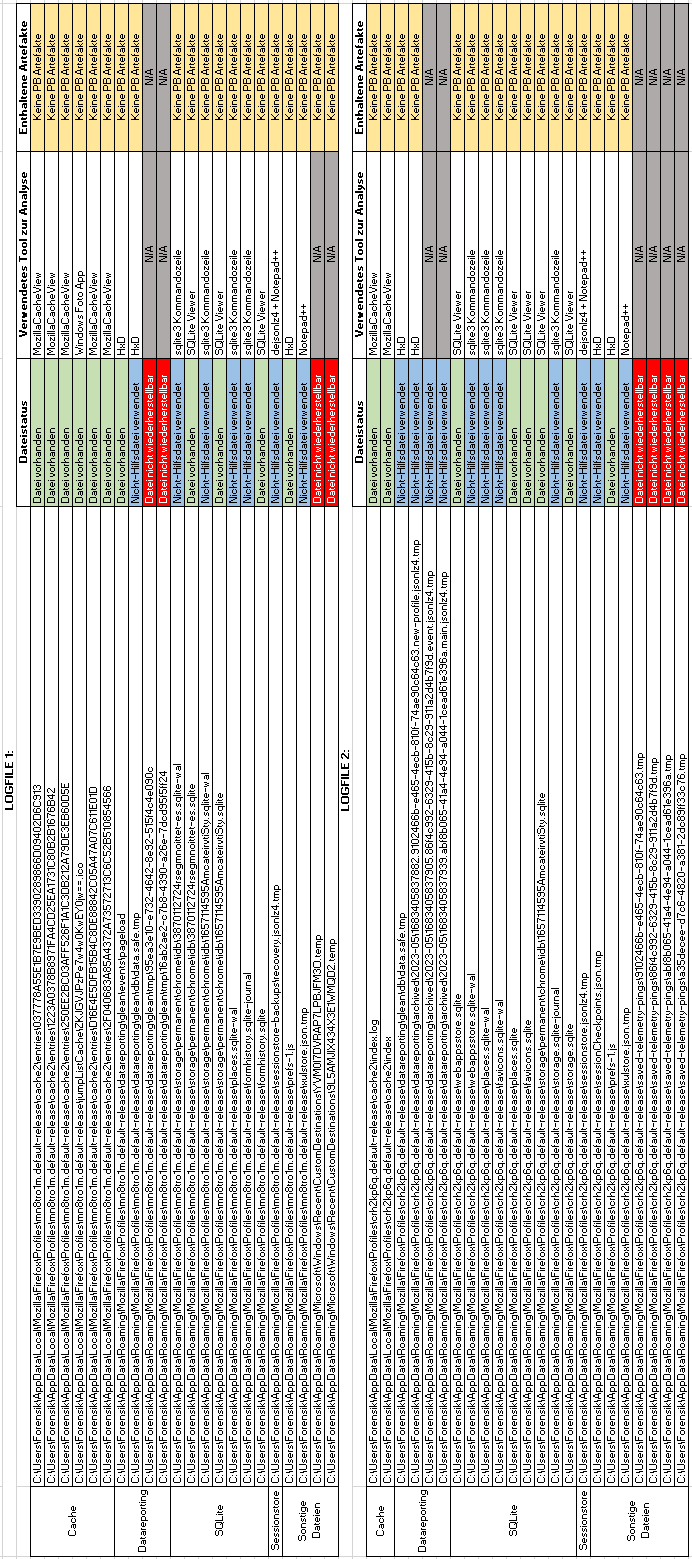
\includegraphics{bilder/firefox-all-write-operations.png}}}
%
%\end{figure}

Diese Dateien können mit dem Tool MZCacheView eingelesen werden.
Wie in Abbildung \ref{img:mzcacheview} gezeigt, konnten im Firefox Cache-Ordner des Festplatten-Images vom zweiten Snapshot drei JSON Dateien identifiziert werden. Dabei handelt es sich um Zertifikatsdateien, die von der \textit{One Certificate Revocation List} stammen, einem Mechanismus von Firefox zur Überprüfung von Zertifikaten. In keinem der Zertifikate konnten mit HxD Private-Browsing-Artefakte oder besuchte Seiten gefunden werden. \cite{TechSupportGuy.05.06.2023}
Weiterhin befindet sich im Cache das HTML-Dokument der Firefox Datenschutzseite, welche sich beim ersten Start des Browsers automatisch öffnete, siehe Abschnitt \ref{subsection:methodik-vorbereitung-browsing-szenario}.
Weitere Cache Dateien konnten in keinem Festplatten-Image gefunden werden.
\begin{figure}[h!]
	\resizebox{\linewidth}{!}{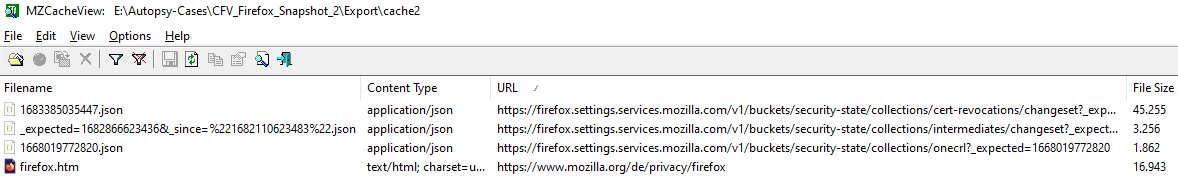
\includegraphics{bilder/firefox-cache.png}}
	\caption{Firefox: Mit MZCacheView eingelesene Cache-Dateien}
	\label{img:mzcacheview}
\end{figure}
Die Indexdatei \texttt{$\backslash$cache2$\backslash$index} dient als Datenbank im Cache. Sie ermöglicht es dem Firefox-Browser, schnell auf die zwischengespeicherten Ressourcen zuzugreifen und diese effizient zu verwalten. In diese Datei wurde beim Schließen des Browsers geschrieben. Sowohl mit HxD als auch dem Tool FirefoxCache2 konnten keine PB-Artefakte identifiziert werden.

Schließlich enthält die Datei \texttt{$\backslash$jumpListCache$\backslash$ZKJGVJPzPe7w4w0KwEY0jw==.ico} ein $64x64$ Pixel großes Mozilla Logo. Dieses Logo ist keinem Schritt des Browsing-Szenarios zuzuordnen und ist vermutlich auf die automatisch geöffnete Datenschutzhinweisseite zurückzuführen.

\paragraph*{Datareporting}
Dateien im Ordner \texttt{$\backslash$datareporting$\backslash$glean$\backslash$db} sind Teil des Glean-Systems, das für die Sammlung von Telemetriedaten und deren Übermittlung an Mozilla verwendet wird. \cite{GitHub.05.06.2023}
Die Datei \texttt{data.safe.bin} enthält verschlüsselte und anonyme Informationen über die Nutzung des Browsers. In HxD konnten keine PB-Artefakte in den Dateien gefunden werden. 

Dateien im Format \texttt{$\backslash$datareporting$\backslash$glean$\backslash$db$\backslash$<Profilname>.new-profile.jsonlz4} speichern Informationen über das Firefox-Profil, das von Glean verwendet wird. In diese Dateien wurde erst nach dem Browsing-Szenario, beim Schließen des Browsers geschrieben. Diese Dateien im proprietären \textit{jsonlz4}-Format lassen sich mit dem Tool dejsonlz4 dekomprimieren. Die entstandene JSON Datei wurde mit dem Notepad++ JSON Plugin untersucht. Dabei konnten keine PB-Artefakte gefunden werden.

\paragraph*{Sessionstore}
Die Datei \texttt{$\backslash$sessionstore-backups$\backslash$recovery.jsonlz4} enthält eine Sicherungskopie der vorherigen Sitzung. Sie wird erstellt, wenn der Firefox-Browser nach einem Absturz oder einem unerwarteten Beenden neu gestartet wird. 
Jefferson Scher entwickelte das Online-Tool \textit{Session History Scrounger for Firefox} zur Analyse dieser \grqq{}Sessionstore-Backup\grqq{} Dateien. \cite{JeffersonScher.29.11.2020}
Wie in Abbildung \ref{img:firefox-session-history-scrounger} gezeigt, enthielt die Datei sowohl im Festplatten-Image 2 (Logfile 1) und 3 (Logfile 2) nur die automatisch geöffnete Seite der Firefox Datenschutzhinweise.
\begin{figure}[h!]
	\resizebox{\linewidth}{!}{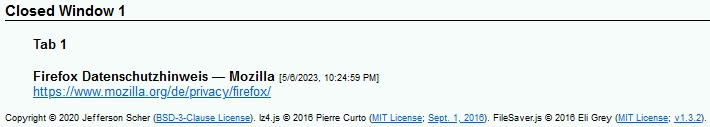
\includegraphics{bilder/firefox-sessionstore.png}}
	\caption{Firefox: Sitzungsdatei \texttt{recovery.jsonlz4}, geöffnet mit dem \grqq{}Session History Scrounger for Firefox\grqq{}}
	\label{img:firefox-session-history-scrounger}
\end{figure}

\paragraph*{Sonstige Dateien}
In der Datei \texttt{prefs-1.js} werden benutzerspezifische Einstellungen und Konfigurationen für den Firefox-Browser gespeichert. Die Datei enthält Präferenzen des Benutzers in Form von JavaScript-Objekten. Es konnten in den Dateien beider Logfiles mit HxD keine PB-Artefakte gefunden werden. 
Schließlich speichert die Datei \texttt{xulstore.json} benutzerspezifische Anpassungen und Konfigurationen des Firefox-Browsers. In der Datei konnten in den Festplatten-Images beider Logfiles mit Notepad++ keine PB-Artefakte gefunden werden. \cite{mozillazine.29.12.2022}

\subsubsection*{SQLite-Datenbanken}
\label{appendix:firefox-sqlite}
Wie in Abschnitt \ref{subsection:methodik-datenanalyse-commonlocations} erwähnt, werden SQLite-Datenbanken als Datenstrukturen für Nutzerdaten detailliert und getrennt von den Schreiboperationen der Process Logfiles untersucht. Mithilfe der Process Monitor Logfiles wurden zunächst die in Tabelle \ref{tab:firefox-sqlite-dbs-explained} dargestellten SQLite-Datenbanken für Firefox identifiziert:
\begin{table}[h!]
\centering
\caption{Firefox: Veränderte SQLite-Datenbanken und deren Verwendungszwecke}
\label{tab:firefox-sqlite-dbs-explained}
\resizebox{\linewidth}{!}{
\begin{tabular}{|l|l|lll}
\cline{1-2}
\textbf{Datenbank}                        & \textbf{Gespeicherte Daten \cite{GitHub.08.04.2019}}                                                                                             &  &  &  \\ \cline{1-2}
\textit{places.sqlite}                    & Informationen über Lesezeichen und Verlauf \\&Zu jeder besuchten Webseite: URL, Seitentitel, Zeitstempel des Besuchs etc.  &  &  &  \\ \cline{1-2}
\textit{cookies.sqlite}                   & Von besuchten Webseiten verwendete Cookies.                                                                             &  &  &  \\ \cline{1-2}
\textit{storage.sqlite}                   & Diverse Webdaten, z. B. Indexed-Datenbanken,\\&Offline-Cache-Daten und andere lokale Speicherinformationen                &  &  &  \\ \cline{1-2}
\textit{favicons.sqlite}                  & Enhtält Favicons (kleine Symbole in der Adressleiste)\\&um besuchte Webseiten visuell zu identifizieren                   &  &  &  \\ \cline{1-2}
\textit{webappsstore.sqlite}              & Speichert Informationen über installierte Webanwendungen\\&im Firefox-Browser, z.B. Berechtigungen und Einstellungen      &  &  &  \\ \cline{1-2}
\textit{1657114595AmcateirvtiSty.sqlite}  & Datenspeicher für Activity Stream, eine personalisierte Übersicht\\&über Browser-Aktivitäten beim Öffnen eines neuen Tabs &  &  &  \\ \cline{1-2}
\textit{3870112724rsegmnoittet-es.sqlite} & Datenspeicher für Remote Settings, eine zentrale Verwaltung\\&von benutzerspezifischen Browsereinstellungen               &  &  &  \\ \cline{1-2}
\end{tabular}
}
\end{table}

Entsprechend der Methodik in Kapitel \ref{subsubsection:methodik-datenanalyse-commonlocations-sqlitedbs} wurde jede SQLite-Datenbank aus den Festplatten-Images aller vier Snapshots extrahiert und verglichen.
Die Ergebnisse sind in Tabelle \ref{tab:firefox-veraenderte-sqlitedbs} dargestellt.

\begin{table}[h!]
\centering
\caption{Veränderung der Firefox SQLite-Datenbanken während der Versuchsdurchführung}
\label{tab:firefox-veraenderte-sqlitedbs}  
\resizebox{\linewidth}{!}{
\begin{tabular}{|l|c|cc|cc|cc|}
\hline
\multicolumn{1}{|c|}{}                                     &                                                                                                    & \multicolumn{2}{c|}{\textbf{\begin{tabular}[c]{@{}c@{}}Nach Browsing-Szenario, \\ Browser geöffnet (S2)\end{tabular}}}                                                                                                                              & \multicolumn{2}{c|}{\textbf{\begin{tabular}[c]{@{}c@{}}Nach Browsing-Szenario, \\ Browser geschlossen (S3)\end{tabular}}}                                                                                                            & \multicolumn{2}{c|}{\textbf{\begin{tabular}[c]{@{}c@{}}VM \\ heruntergefahren (S4)\end{tabular}}} \\ \cline{3-8} 
\multicolumn{1}{|c|}{\multirow{-2}{*}{\textbf{Dateiname}}} & \multirow{-2}{*}{\textbf{\begin{tabular}[c]{@{}c@{}}Vor Browsing \\ Szenario\\ (S1)\end{tabular}}} & \multicolumn{1}{c|}{\textbf{Vor WAL}}                                                                                                      & \textbf{Nach WAL}                                                                                      & \multicolumn{1}{c|}{\textbf{Vor WAL}}                                                                                       & \textbf{Nach WAL}                                                                                      & \multicolumn{1}{c|}{\textbf{Vor WAL}}                     & \textbf{Nach WAL}                     \\ \hline
places.sqlite                                              & \cellcolor[HTML]{C0C0C0}N/A                                                                        & \multicolumn{1}{c|}{\cellcolor[HTML]{F56B00}\begin{tabular}[c]{@{}c@{}}Initialisiert \\ (Datenschutz-Seite)\end{tabular}}                  & \cellcolor[HTML]{FE996B}                                                                               & \multicolumn{1}{c|}{\cellcolor[HTML]{F56B00}Indizes aktualisiert}                                                           & \cellcolor[HTML]{FE996B}                                                                               & \multicolumn{2}{c|}{\cellcolor[HTML]{FE996B}}                                                     \\ \cline{1-3} \cline{5-5}
cookies.sqlite                                             & \cellcolor[HTML]{C0C0C0}N/A                                                                        & \multicolumn{1}{c|}{\cellcolor[HTML]{FFCE93}}                                                                                              & \cellcolor[HTML]{FE996B}                                                                               & \multicolumn{1}{c|}{\cellcolor[HTML]{FE996B}}                                                                               & \cellcolor[HTML]{FE996B}                                                                               & \multicolumn{2}{c|}{\cellcolor[HTML]{FE996B}}                                                     \\ \cline{1-2}
storage.sqlite                                             & \cellcolor[HTML]{C0C0C0}N/A                                                                        & \multicolumn{1}{c|}{\cellcolor[HTML]{FFCE93}}                                                                                              & \cellcolor[HTML]{FE996B}                                                                               & \multicolumn{1}{c|}{\cellcolor[HTML]{FE996B}}                                                                               & \cellcolor[HTML]{FE996B}                                                                               & \multicolumn{2}{c|}{\cellcolor[HTML]{FE996B}}                                                     \\ \cline{1-2}
favicons.sqlite                                            & \cellcolor[HTML]{C0C0C0}N/A                                                                        & \multicolumn{1}{c|}{\multirow{-3}{*}{\cellcolor[HTML]{FFCE93}\begin{tabular}[c]{@{}c@{}}Initialisiert \\ (Nur Spaltennamen)\end{tabular}}} & \multirow{-4}{*}{\cellcolor[HTML]{FE996B}\begin{tabular}[c]{@{}c@{}}keine \\ Veränderung\end{tabular}} & \multicolumn{1}{c|}{\multirow{-3}{*}{\cellcolor[HTML]{FE996B}\begin{tabular}[c]{@{}c@{}}keine \\ Veränderung\end{tabular}}} & \cellcolor[HTML]{FE996B}                                                                               & \multicolumn{2}{c|}{\cellcolor[HTML]{FE996B}}                                                     \\ \cline{1-5}
webappsstore.sqlite                                        & \cellcolor[HTML]{C0C0C0}N/A                                                                        & \multicolumn{1}{c|}{\cellcolor[HTML]{C0C0C0}N/A}                                                                                           & \cellcolor[HTML]{C0C0C0}N/A                                                                            & \multicolumn{1}{c|}{\cellcolor[HTML]{FFCE93}\begin{tabular}[c]{@{}c@{}}Initialisiert \\ (Nur Spaltennamen)\end{tabular}}    & \cellcolor[HTML]{FE996B}                                                                               & \multicolumn{2}{c|}{\cellcolor[HTML]{FE996B}}                                                     \\ \cline{1-5}
formhistory.sqlite                                         & \cellcolor[HTML]{C0C0C0}N/A                                                                        & \multicolumn{1}{c|}{\cellcolor[HTML]{FFCE93}\begin{tabular}[c]{@{}c@{}}Initialisiert \\ (Nur Spaltennamen)\end{tabular}}                   & \cellcolor[HTML]{FE996B}                                                                               & \multicolumn{1}{c|}{\cellcolor[HTML]{FE996B}keine Veränderung}                                                              & \cellcolor[HTML]{FE996B}                                                                               & \multicolumn{2}{c|}{\cellcolor[HTML]{FE996B}}                                                     \\ \cline{1-3} \cline{5-5}
1657114595AmcateirvtiSty.sqlite                            & \cellcolor[HTML]{C0C0C0}N/A                                                                        & \multicolumn{1}{c|}{\cellcolor[HTML]{CE6301}\begin{tabular}[c]{@{}c@{}}Initialisiert \\ (\grqq{}origin\grqq{}: \grqq{}chrome\grqq{})\end{tabular}}                 & \cellcolor[HTML]{FE996B}                                                                               & \multicolumn{1}{c|}{\cellcolor[HTML]{F56B00}\begin{tabular}[c]{@{}c@{}}Binärdaten, \\ keine PB-Artefakte\end{tabular}}      & \cellcolor[HTML]{FE996B}                                                                               & \multicolumn{2}{c|}{\cellcolor[HTML]{FE996B}}                                                     \\ \cline{1-3} \cline{5-5}
3870112724rsegmnoittet-es.sqlite                           & \cellcolor[HTML]{C0C0C0}N/A                                                                        & \multicolumn{1}{c|}{\cellcolor[HTML]{CE6301}\begin{tabular}[c]{@{}c@{}}Initialisiert \\ (\grqq{}origin\grqq{}: \grqq{}chrome\grqq{})\end{tabular}}                 & \multirow{-3}{*}{\cellcolor[HTML]{FE996B}\begin{tabular}[c]{@{}c@{}}keine \\ Veränderung\end{tabular}} & \multicolumn{1}{c|}{\cellcolor[HTML]{FE996B}keine Veränderung}                                                              & \multirow{-12}{*}{\cellcolor[HTML]{FE996B}\begin{tabular}[c]{@{}c@{}}keine \\ Veränderung\end{tabular}} & \multicolumn{2}{c|}{\multirow{-12}{*}{\cellcolor[HTML]{FE996B}keine Veränderung}}                  \\ \hline
\end{tabular}
}
\end{table}

Unmittelbar nach der Installation von Firefox (Snapshot 1) existierte noch keine der SQLite-Dateien.

Nach dem Browsing-Szenario (Snapshot 2) wurden alle SQLite-Datenbanken außer \texttt{webappsstore.sqlite} 
initialisiert. Dabei wurden in \texttt{places.sqlite} die automatisch im normalen Modus geöffnete Firefoxseite der Datenschutzhinweise eingetragen. 
Die restlichen Datenbanken wurden leer initialisiert, nur die Spaltennamen wurden definiert.
Der Inhalt aller initialisierten Datenbanken blieb nach Durchführung von PRAGMA WAL Checkpoints unverändert.

Nach Schließen des Browsers (Snapshot 3) wurden in \texttt{places.sqlite} die Indizes der eingetragenen Seiten aktualisiert. Die SQLite-Datenbank \texttt{1657114595AmcateirvtiSty.sqlite} erhielt ein binäres Datenobjekt als Eintrag. Bei der Untersuchung mit HxD konnten keine Artefakte gefunden werden. Weiterhin wurde \texttt{webappsstore.sqlite} leer initialisiert. Die restlichen Daten blieben im Vergleich mit Snapshot 2 unverändert. Ebenfalls veränderte sich nicht der Inhalt nach Durchführung von PRAGMA WAL Checkpoints.

Weder nach dem Herunterfahren der VM (Snapshot 4), noch nach Durchführung der PRAGMA WAL Checkpoints, entstanden Änderungen in den SQLite-Datenbanken.	
Somit wurden in den SQLite-Datenbanken von Firefox keine zurückverfolgbaren PB-Artefakte im privaten Modus hinterlassen.

\subsubsection*{Zusammenfassung Firefox Common Locations}
Mithilfe der Process Monitor Logfiles wurde festgestellt, dass sowohl während des Browsing-Szenarios (Logfile 1) als auch danach (Logfile 2) Inhalte in Dateien geschrieben wurden. Wie in Abbildung \ref{chart:firefox-writefile-logfile1v2} dargestellt, gab es mit Ausnahme der \textit{Datareporting} Dateien in Logfile 1 stets mehr oder gleich viele Schreiboperationen wie in Logfile 2. Keine der Schreiboperation hinterließ Private-Browsing-Artefakte.

\begin{figure}[h!]
	\begin{tikzpicture}
	\begin{axis}[
	xbar, 
	xmin=0,
	width=12cm, 
	height=12cm, 
	xlabel={Anzahl Schreiboperationen},
	y=1.2cm,
	%					0  					1			   2 		  3			 4
	%yticklabels={Sonstige Dateien, Sessionstore-Backup, SQLite, Datareporting, Cache},
	%ytick=data,
	symbolic y coords={Sonstige Dateien,Sessionstore-Backup,SQLite,Datareporting,Cache},
	ytick=data,
	%symbolic y coords={Sonstige-Dateien,Sessionstore-Backup,SQLite,Datareporting,Cache},
	%ytick=data,
	nodes near coords, nodes near coords align={horizontal},
	yminorgrids = true,minor tick num=1
	]
	\addplot coordinates {(2,Sonstige Dateien) (1,Sessionstore-Backup) (7,SQLite) (2,Datareporting) (4,Cache)};
	\addplot coordinates {(2,Sonstige Dateien) (1,Sessionstore-Backup) (3,SQLite) (4,Datareporting) (2,Cache)};
	
	\legend{Logfile 1, Logfile 2}
	\end{axis}
	\end{tikzpicture}
	\caption{Firefox: Anzahl Schreiboperationen Logfile 1 vs Logfile 2, geordnet nach Kategorie}
	\label{chart:firefox-writefile-logfile1v2}
\end{figure}

%Literatur:
%	o no traces were found in “common locations” \cite{Montasari.2015}
%		>  “places.sqlite”, “webappsstore. sqlite”, “sessionstore.bak”, “search.json” and “nssckbi.dll”
%	o	Safebrowsing: Alle Dateien in /safebrowsing-updating/ nicht relevant. Dort nur .vlpset und .sbstore Dateien. Speichern 256-Bit Hash von URLs, die auf SafeSearch Blacklist stehen 
%	o	Cache-Dateien: drei Caches: startupCache, jumpListCache (beide enthalten Binärdateien ohne Browsing-Artefakte) und cache2 (können mit MZCacheView untersucht werden, enthalten keine Browsing-Artefakte)
%	o	SQLite-Datenbanken: Sqlite Dateien erst ohne WAL Dateien untersuchen, Danach mit sqlite3 Konsole: WAL in Datenbank schreiben mit: PRAGMA wal\_checkpoint; places.sqlite besonders relevant, da dort Browser in public Modus Browsing URLs verwaltet (Am besten hier vergleich mit Public Browsing machen)	
%		> \cite{Fayyad.2021} for Mozilla Firefox, 7 database files were recovered: cookies.sqlite-shm, places.sqlite-shm, prefs.js etc.
%		> \cite{Muir.2019} The two SQLite databases used by Firefox to track cookies and history (cookies.sqlite und places.sqlite) were both recoverable from the file system after deletion	
%		Ergebnisse stehen im Gegensatz zu \cite{Hedberg.2013} :
%			o	Chrome und Firefox: Einträge in places.sqlite + history.sqlite DB gefunden während PB! (Noch aktuell??)
%		Sonderfall: SQlite DB-Crash \cite{Hedberg.2013}
%			> WAL Files/Journal Files bei Crash gefunden -> Kann genutzt werden um zu beweisen, dass privater Browser genutzt wurde
%			> Daher: WAL Rollback mit sqlite3	
%	o	Jsonlz4 \& balkz4: Enthalten komprimierte Firefox-Sessions, jsonlz4 Dateien können mit Tool \grqq{}entkomprimiert\grqq{} werden: https://www.jeffersonscher.com/ffu/scrounger.html

\subsection{Uncommon Locations}
\label{subsection:appendix-firefox-uncommon-locations}

\subsubsection*{Analyse mit Autopsy - Kategorisierte Dateien}
\label{subsubsection:appendix-firefox-uncommon-locations-autopsy}

Beim Vergleich der Festplattenabbilder wurde festgestellt, dass ein Festplatten-Image stets die kategorisierten Dateien des Festplatten-Images des vorherigen Snapshots enthielt. Somit enthält das Festplatten-Image von Snapshot 4 alle kategorisierten Dateien der vorherigen Snapshots.

\paragraph*{Web Bookmarks}
Bereits vor Durchführung des Browsing-Szenarios enthielt Firefox im ersten Snapshot die in Abbildung \ref{img:firefox-web-bookmarks} dargestellte Bing Startseite als gespeichertes Lesezeichen. In den restlichen Snapshots 2 bis 4 blieb diese Kategorie unverändert.
\begin{figure}[h!]
	\centerline{\resizebox{\linewidth}{!}{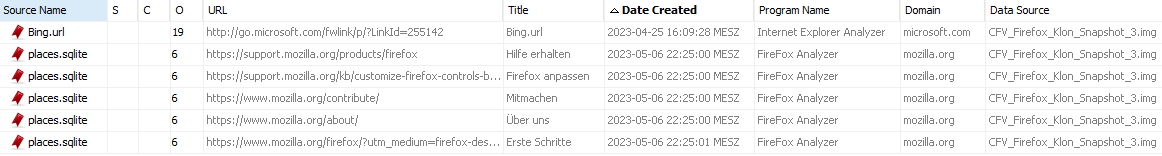
\includegraphics{bilder/cfv_firefox_autopsy_web_bookmarks.png}}}
	\caption{Firefox: Von Autopsy als \grqq{}Web Bookmarks\grqq{} kategorisierte Dateien}
	\label{img:firefox-web-bookmarks}  
\end{figure}

\paragraph*{Web Cookies}
Die Kategorie \grqq{}Web Cookies\grqq{} enthält bereits vor Beginn des Browsing-Szenarios zehn in Abbildung \ref{img:firefox-web-cookies} gezeigte Cookie-Einträge in der Datei \texttt{WebCacheV01.dat}. Dabei handelt es sich um eine Datenbank des Microsoft Edge Browsers zur Speicherung von Nutzerdaten. Diese Datei verhält sich ähnlich wie die in diesem Versuch relevanten SQLite-Dateien. Bei den Einträgen handelt es sich um Cookies für Bing und die Outlook Webseite, obwohl diese Seiten nie in Microsoft Edge geöffnet wurden. In den Snapshots 2 bis 4 kamen keine weiteren Einträge in dieser Kategorie hinzu.
\begin{figure}[h!]
	\centerline{\resizebox{\linewidth}{!}{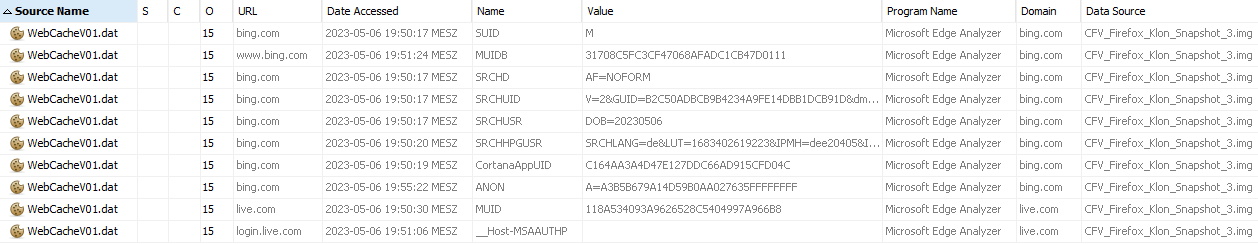
\includegraphics{bilder/cfv_firefox_autopsy_web_cookies.png}}}
	\caption{Firefox: Von Autopsy als \grqq{}Web Cookies\grqq{} kategorisierte Dateien}
	\label{img:firefox-web-cookies}  
\end{figure}

\paragraph*{Web History}
Die Kategorie \grqq{}Web History\grqq{} listet alle Dateien mit gespeichertem Suchverlauf auf. Vor Beginn des Browsing-Szenarios (Snapshot 1) enthält die Kategorie zwei Einträge zur Outlook Webseite in der Datei \texttt{WebCacheV01.dat}. Nach Durchführung des Browsing-Szenarios (Snapshot 2) wurde ein Eintrag in der \texttt{places.sqlite} Datenbank hinzugefügt. Dabei handelt es sich um die automatisch im normalen Browsingmodus geöffnete Firefox-Standardseite über Datenschutzhinweise. Dies deckt sich mit den Beobachtungen der Common Locations in Anhang \ref{subsection:appendix-firefox-common-locations}. Darüber hinaus enthält dieser Snapshot für die Datei \texttt{WebCacheV01.dat} den Eintrag \texttt{file:///Z:/Logfile\_1}. Dabei handelt es sich um das Process Monitor Logfile, das gemäß Methodik in Abschnitt \ref{section:methodik-vorbereitung} über den gemeinsamen VM-Ordner zum Analyse-Rechner transportiert wurde. Ergänzt wird die Kategorie nach Schließen des Browsers (Snapshot 3) durch den Eintrag \texttt{file:///Z:/Logfile\_2}, dem zweiten Process Monitor Logfile. Nach Herunterfahren der virtuellen Maschine (Snapshot 4) werden in dieser Katgeorie keine neuen Dateien erfasst. Die kategorisierten Dateien sind in Abbildung \ref{img:firefox-web-history} dargestellt.
\begin{figure}[h!]
	\centerline{\resizebox{\linewidth}{!}{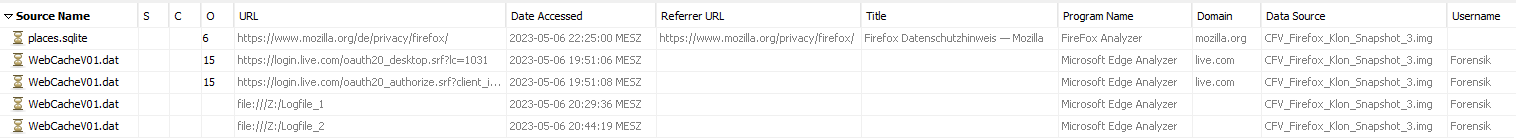
\includegraphics{bilder/cfv_firefox_autopsy_web_history.png}}}
	\caption{Firefox: Von Autopsy als \grqq{}Web History\grqq{} kategorisierte Dateien}
	\label{img:firefox-web-history}  
\end{figure}

\paragraph*{Web Categories}
Diese Kategorie klassifiziert im Speicherabbild gefundene Browsing-Artefakte nach Inhalt.
Vor Beginn des Browsing-Szenarios (Snapshot 1) werden hier bereits zwei in Abbildung \ref{img:firefox-web-categories} dargestellte Einträge in der Datei \texttt{WebCacheV01.dat} aufgelistet. Der Eintrag \texttt{bing.com} wird als \grqq{}Suchmaschine\grqq{} klassifiziert und \texttt{live.com} als \grqq{}Web-Email\grqq{}.
Wie oben erwähnt, wurden beide Seiten nie aufgerufen. Es gab keine zusätzlichen Einträge in dieser Kategorie während des restlichen Browsing-Szenarios (Snapshots 2 bis 4).
\begin{figure}[h!]
	\centerline{\resizebox{\linewidth}{!}{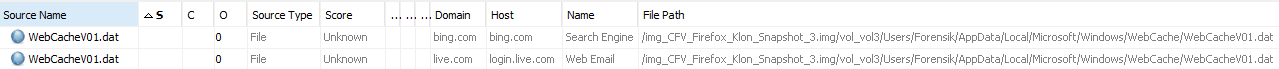
\includegraphics{bilder/cfv_firefox_autopsy_web_categories.png}}}
	\caption{Firefox: Von Autopsy als \grqq{}Web Categories\grqq{} kategorisierte Dateien}
	\label{img:firefox-web-categories}  
\end{figure}

Somit wurden in allen Kategorien ausschließlich Browsing-Artefakte des Edge Browsers in der Datei \texttt{WebCacheV01.dat} gefunden, sowie ein Eintrag in der Firefox SQLite-Datenbank \texttt{places.sqlite}. In keiner der Kategorien konnten Private-Browsing-Artefakte identifiziert werden. Die von Autopsy erkannte Firefox-Standardseite deckt sich mit den Ergebnissen der Common Locations. Die aufgelisteten Einträge in der Datei \texttt{WebCacheV01.dat} sind nicht auf Schritte des Browsing-Szenarios zurückzuführen. Die Einträge sind bereits im ersten Snapshot enthalten, obwohl vor Beginn des Browsing-Szenarios keine Browseraktivitäten durchgeführt wurden. Weiterhin enthält diese Datei Einträge über die Process Monitor Logfiles, welche über einen gemeinsamen VM-Ordner zum Rechner transportiert wurde, auf dem die virtuelle Maschine läuft.

%Literatur:
%	o	Autopsy Keywortsuche: 
%		>	In alles Snapshots ergebnislos (keine Keyword-Hits
%		-->	In Literatur: Autoren fanden Ergebnisse in pagefile.sys 
%			> Autopsy: websites and some of the keywords found in hidden file called “pagefile.sys” \cite{Mahlous.2020}
%			o \cite{Montasari.2015} traces were found in: 
%				> However, on investigating the “pagefile.sys”, some entries were discovered
%				> Using the “data carving” technique, profile picture was recovered
%			o \cite{Said.2011} 
%				> Examining pagefile.sys showed some positive hits 			
%		--> Evtl. hier zeigen, was gefunden werden kann, wenn RAM reduziert
%		--> Aber auf Problem hinweisen, dass gefundener String in pagefile nicht direkt Browser zugeordnet werden kann
%		> \cite{Gabet.2018}	Firefox only produced three recoverable artefacts as reported by both tools (FTK, Autopsy) --> Artefakte werden nicht genannt!
%		> \cite{Muir.2019} Autopsy Keyword Suche nach Suchbegriffen: unallocated space
%		> Autopsy Carving Module (\$Carved): \cite{Muir.2019}
%			•	When searching for the string ’clot’ from the browsing protocol, six .dll, .edb and .reg files were discovered in unallocated space.
%			•	Further searching of unallocated space uncovered references to the Tor installation directory and the obfs4 bridging IP addresses
%			•	browsing data found in NTUSER.DAT was also replicated in unallocated space.
%	o	Autopsy PlugIns:
%		>	*** TODO: Hier Liste mit PlugIns ***

\subsection{Registry}
\label{subsection:appendix-firefox-registry}

\subsubsection*{Process Monitor SetValue Operations}
\label{subsubsection:appendix-firefox-registry-processmonitorsetvalue}
Als Teil der Common Locations werden für Firefox alle Registry \grqq{}SetValue\grqq{} Schreiboperationen der beiden Process Monitor Logfiles untersucht.

In beiden Logfiles wurden zwei Kategorien von Registry Keys geschrieben: \textit{PreXULSkeletonUISettings} und \textit{Business Activity Monitoring}. In Abbildung \ref{chart:firefox-registy-css-vs-bam} ist der Anteil der Schreiboperationen je Kategorie für beide Logfiles gezeigt.
\begin{figure}[h!]
	\resizebox{\linewidth}{!}{
	\begin{tikzpicture}
		\begin{axis}[
		xbar stacked,
		width=18cm, 
		height=12cm, 
%		ylabel style={align=center}, ylabel=RAM-Dump 1,
		y=1cm,
		enlarge y limits={abs=2*\pgfplotbarwidth},
		symbolic y coords={Logfile 2,Logfile 1},
		ytick=data,
		xticklabels={,,},
        xmin = 0,
        xmax = 40,
		nodes near coords, 
		nodes near coords align={horizontal},
		legend style={
			at={(0.5,-0.1)},
			anchor=north
		},
		every node near coord/.style={xshift=-0.2cm},
		legend columns=2,
		scaled x ticks=false
		]
			\addplot coordinates {
			(10,Logfile 2) (10,Logfile 1)
			};
			\addplot coordinates {
			(1,Logfile 2) (27,Logfile 1)
			};
			\legend{PreXULSkeletonUISettings (CSS), Business Activity Monitoring (BAM)}
		\end{axis}
	\end{tikzpicture}
	}	
	\caption{Firefox: Registry \grqq{}SetValue\grqq{} Operationen in den Process Monitor Logfiles 1 und 2}
	\label{chart:firefox-registy-css-vs-bam}
\end{figure}

%\begin{figure}[h!]
%	\centerline{\resizebox{\linewidth}{!}{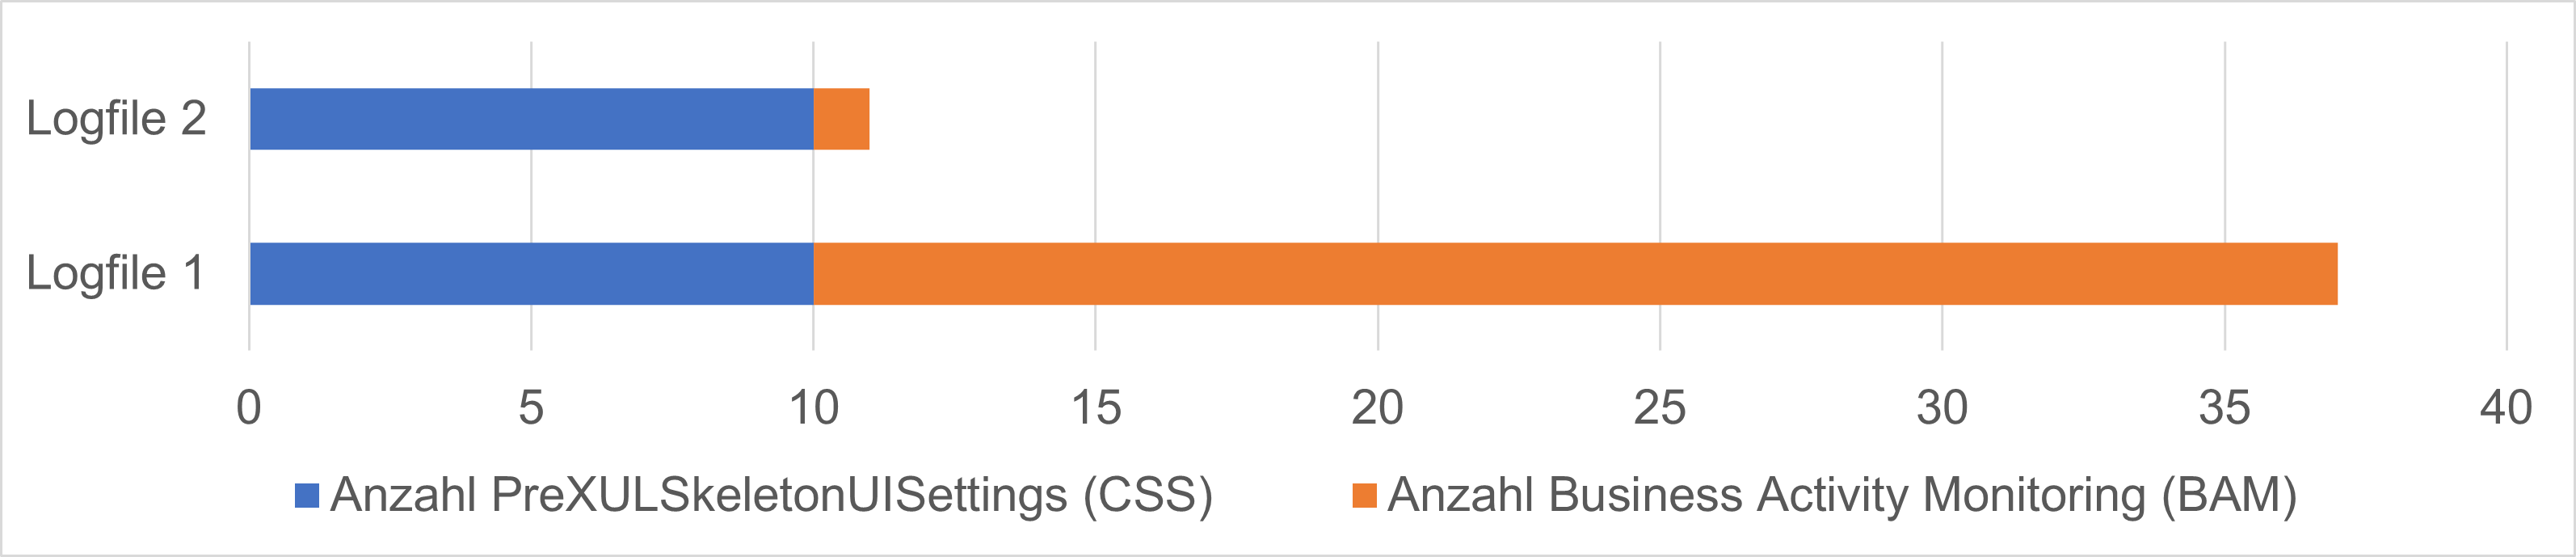
\includegraphics{bilder/firefox-registry-stacked-bar-chart.png}}}
%	\label{chart:final-criteria}  
%	\caption{Comparison of found PB artifacts between RAM Dumps}
%\end{figure}

\paragraph*{PreXULSkeletonUISettings}
Der \textit{PreXULSkeletonUISettings} Registry Key enthält Einstellungen für die Benutzeroberfläche (UI) des Firefox-Browsers, insbesondere für das sogenannte \textit{Skeleton UI}, eine vereinfachte Benutzeroberfläche, die während des Ladens des Browsers angezeigt wird, bevor die vollständige Benutzeroberfläche geladen ist. 
PreXULSkeletonUISettings Registry Keys haben das Format \texttt{HKCU$\backslash$SOFTWARE$\backslash$Mozilla$\backslash$Firefox$\backslash$\\PreXULSkeletonUISettings$\backslash$<Absoluter Firefox Installationspfad>$\backslash$firefox.exe\\|<Skeleton UI Setting>}.
Somit enthält der Key den absoluten Installationspfad von Firefox gefolgt von einer Skeleton UI Einstellung. Nachfolgend sind alle möglichen UI Einstellungen aufgelistet, gefolgt vom Datentyp des Keys. \cite{Mills.2021}
\begin{itemize}
	\item ScreenX (DWORD)
	\item ScreenY (DWORD)
	\item Width (DWORD)
	\item Height (DWORD)
	\item Maximized (DWORD)
	\item Flags (DWORD)
	\item CssToDevPixelScaling (REG\_BINARY)
	\item UrlbarCSSSpan (REG\_BINARY)
	\item SearchbarCSSSpan (REG\_BINARY)
	\item SpringsCSSSpan (REG\_BINARY)
\end{itemize}
Somit enthalten die Keys nur Daten zur Formatierung und Struktur der grafischen Oberfläche. Es wurden keine PB-Artefakte geschrieben.

\paragraph*{Business Activity Monitoring}
\textit{Business Activity Monitoring}, kurz \textit{BAM} ist eine weitgehend undokumentierte Windows Funktion, die im Hintergrund ausgeführte Programme steuert.
Der Registry Key hat das Format \texttt{HKLM$\backslash$System$\backslash$CurrentControlSet$\backslash$Services$\backslash$bam$\backslash$State$\backslash$\\UserSettings$\backslash$<SID>$\backslash$Device$\backslash$HarddiskVolume2$\backslash$<Absoluter Firefox\\ Installationspfad>$\backslash$firefox.exe} und den Datentyp REG\_BINARY.
Jeder Schlüssel wird durch die Sicherheits-ID (SID) des Benutzers identifiziert.
Ein BAM Registry Key schreibt für alle ausgeführten Programme -- hier Firefox -- den Zeitstempel der letzten Ausführung.
PB-Artefakte sind dabei nicht enthalten. \cite{MandiOhlinger.05.06.2023, InfoSecNotes.05.06.2023}

\subsubsection*{Stringsuche in Registry Hives}
Gemäß Methodik in Abschnitt \ref{subsection:methodik-datenanalyse-registry} wird die Firefox Registry als Uncommon Location behandelt, indem über alle auf der Festplatte vorhandenen Registry Datenbanken, den Registry Hives, eine Stringsuche durchgeführt wird, ohne die Struktur der Hives zu beachten. 
Dazu wurden sowohl die System-Hives als auch die User-Hives aus Tabelle \ref{tab:windows-Registry Hives} aus jedem Festplatten-Image extrahiert und mithilfe des Registry Explorers nach PB-Artefakten durchsucht.
Dabei wurde in keinem Snapshot in keinem Hive ein PB-Artefakt gefunden.

%Literatur:
%	>	Auf Autor verweisen: angeblich in Shellactivities Ergebnisse. --> Nicht mehr vorhanden in aktueller Version (Verweis auf E-Mail)
%	>	Process Monitor/Regshot zeigen keine relevanten Key-Änderungen
%	> \cite{Muir.2019}: Autopsy Keyword Suche nach Suchbegriffen: Ergebnisse in \%SystemRoot\%Minidump NTUSER.DAT, ntuser.dat.LOG1 (a log of changes to NTUSER.DAT)
%	> Zentral: shellactivites Key:	NTUSER.DAT --> “shellactivities” key \cite{Muir.2019}
%	> \cite{Rochmadi.2017} Detection of registry changes helps to determine what the appropriate plugin is used to search for digital evidence using volatility memory forensic:
%	- RegQueryValue:	HKCU/Software/Microsoft/Windows/CurrentVersion/InternetSettings/Connections/DefaultConnectionSettings
%	- RegCloseValue: 	HKCU/Software/Microsoft/Windows/CurrentVersion/InternetSettings/Connections
%	- IRP\_MJ\_READ: C:/pagefile.sys


%%%%%%%%%%%%%%%%%%%%%%%%%%%%%%%%%%%%%%%%%%%%%%%%%%%%%%%%%%%%
%%%%%%%%%%%%%%%%%%%%%%%%%%%%%%%%%%%%%%%%%%%%%%%%%%%%%%%%%%%%
%%%%%%%%%%%%%%%%%%%%%%%%%%%%%%%%%%%%%%%%%%%%%%%%%%%%%%%%%%%%

\section{Ausführliche Analyse: Tor}\label{section:appendix-tor}

\subsection{Common Locations}
\label{subsection:appendix-tor-common-locations}
\subsubsection*{Process Monitor WriteFile Operations}
\label{subsubsection:appendix-tor-common-locations-writefile-operations}
Bei der Versuchsdurchführung für den Tor-Browser gemäß Kapitel \ref{section:methodik-datensammlung} wurden drei Process Monitor Logfiles erstellt.
Diese Dateien enthalten alle aufgezeichneten Prozessaktivitäten während des Browsing-Szenarios, dem Erzeugen einer \grqq{}Neuen Identität\grqq{} sowie des Schließens des Browsers.
Tabelle \ref{tab:tor-writefile-operations} enthält alle in den Logfiles identifizierten Dateien.
Für jede Datei wurde vermerkt ob und wie sie wiederherstellbar war, mit welchem Tool die Datei analysiert wurde und ob PB-Artefakte enthalten sind.
Die Dateien wurden in die Kategorien \textit{Cache}, \textit{datareporting}, und \textit{Sonstige Dateien} eingeordnet.
In keiner der identifizierten Dateien konnten PB-Artefakte gefunden werden. 

Bei Analyse der Schreiboperationen konnten zwei Datei-Pfade identifiziert werden:
\begin{itemize}
\item \textbf{Caches:} \texttt{C:$\backslash$Users$\backslash$Forensik$\backslash$Desktop$\backslash$Tor Browser$\backslash$Browser$\backslash$TorBrowser$\backslash$\\Data$\backslash$Browser$\backslash$\\Caches$\backslash$profile.default$\backslash$}
\item \textbf{Profile.default:} \texttt{C:$\backslash$Users$\backslash$Forensik$\backslash$Desktop$\backslash$Tor Browser$\backslash$Browser$\backslash$TorBrowser$\backslash$\\Data$\backslash$Browser$\backslash$\\profile.default$\backslash$}
\end{itemize}
In der Tabelle sind die Dateien je nach Speicherort \textit{Caches} (Hellblau) oder \textit{Profile.default} (Dunkelblau) eingefärbt. 

Bei der Auswertung der Process Monitor Logfiles wurde festgestellt, dass alle Schreiboperationen von \grqq{}firefox.exe\grqq{}-Prozessen und nicht \grqq{}tor.exe\grqq{}-Prozessen durchgeführt wurden. Obwohl keine der Dateien PB-Artefakte enthält, werden zum vollständigen Verständnis des Browsers im Sinne der White-Box-Forensik die wichtigsten Dateien im Zusammenhang des Tor-Browsers genauer untersucht.

\paragraph*{Cache}
Der Tor-Browser schreibt eine einzige Cache-Datei \texttt{$\backslash$Caches$\backslash$profile.default$\backslash$\\startupCache$\backslash$startupCache.8.little} im Caches-Pfad. Alle anderen geschriebenen Dateien befinden sich im Profile.default-Pfad.
Die Datei \grqq{}startupCache.8.little\grqq{} ist eine interne Datei, welche erstellt wird, um den Startvorgang des Browsers zu beschleunigen. Sie enthält Informationen über bereits geladene Browser-Komponenten wie JavaScript-Code, CSS-Dateien, Bilder und andere Ressourcen. \cite{MozillaWiki.05.06.2023} 
Bei Untersuchung mit HxD konnten keine PB-Artefakte gefunden werden.

%\newpage
\newgeometry{bottom=2cm,top=0.5cm}
\afterpage{
\begin{landscape}% Landscape page
	\setcounter{page}{70}
%	\thispagestyle{empty}
	\vspace*{1.5cm}
	\hspace*{-1cm}
	\begin{table}[h!]
%	\centering
	\caption{Tor-Browser: Alle \grqq{}WriteFile\grqq{}-Operationen der Logfiles 1, 2-1 und 2-2}
	\label{tab:tor-writefile-operations}
	\vspace{0.5cm}
	\resizebox{\linewidth}{!}{
	\begin{tabular}{cllll}
	\multicolumn{5}{c}{\textbf{LOGFILE 1:}}                                                                                                                                                                                                                                                                                                                                                                                                                                        \\ \hline
	\multicolumn{1}{|c|}{\textbf{Kategorie}}                                                                      & \multicolumn{1}{c|}{\textbf{Dateiname}}                                                                                                        & \multicolumn{1}{c|}{\textbf{Dateistatus}}                               & \multicolumn{1}{c|}{\textbf{Verwendetes Tool zur Analyse}}        & \multicolumn{1}{l|}{\textbf{Enthaltene Artefakte}}              \\ \hline
	\multicolumn{1}{|c|}{\textit{Cache}}                                                                          & \multicolumn{1}{l|}{\cellcolor[HTML]{34CDF9}\textbackslash{}startupCache\textbackslash{}startupCache.8.little}                                 & \multicolumn{1}{l|}{\cellcolor[HTML]{009901}Datei vorhanden}            & \multicolumn{1}{l|}{\cellcolor[HTML]{FFFFFF}HxD}                  & \multicolumn{1}{l|}{\cellcolor[HTML]{F8A102}Keine PB-Artefakte} \\ \hline
	\multicolumn{1}{|c|}{}                                                                                        & \multicolumn{1}{l|}{\cellcolor[HTML]{3190FF}\textbackslash{}datareporting\textbackslash{}glean\textbackslash{}db\textbackslash{}data.safe.bin} & \multicolumn{1}{l|}{\cellcolor[HTML]{009901}Datei vorhanden}            & \multicolumn{1}{l|}{\cellcolor[HTML]{FFFFFF}HxD}                  & \multicolumn{1}{l|}{\cellcolor[HTML]{F8A102}Keine PB-Artefakte} \\ \cline{2-5} 
	\multicolumn{1}{|c|}{\multirow{-2}{*}{\textit{Datareporting}}}                                                & \multicolumn{1}{l|}{\cellcolor[HTML]{3190FF}\textbackslash{}datareporting\textbackslash{}state.json.tmp}                                       & \multicolumn{1}{l|}{\cellcolor[HTML]{FCFF2F}Nicht-temp-Datei verwendet} & \multicolumn{1}{l|}{\cellcolor[HTML]{FFFFFF}Notepad++}            & \multicolumn{1}{l|}{\cellcolor[HTML]{F8A102}Keine PB-Artefakte} \\ \hline
	\multicolumn{1}{|c|}{}                                                                                        & \multicolumn{1}{l|}{\cellcolor[HTML]{3190FF}\textbackslash{}addonStartup.json.lz4.tmp}                                                         & \multicolumn{1}{l|}{\cellcolor[HTML]{FCFF2F}Nicht-temp-Datei verwendet} & \multicolumn{1}{l|}{\cellcolor[HTML]{FFFFFF}dejsonlz4, Notepad++} & \multicolumn{1}{l|}{\cellcolor[HTML]{F8A102}Keine PB-Artefakte} \\ \cline{2-5} 
	\multicolumn{1}{|c|}{}                                                                                        & \multicolumn{1}{l|}{\cellcolor[HTML]{3190FF}\textbackslash{}AlternateServices.txt}                                                             & \multicolumn{1}{l|}{\cellcolor[HTML]{009901}Datei vorhanden}            & \multicolumn{1}{l|}{\cellcolor[HTML]{FFFFFF}Notepad++}            & \multicolumn{1}{l|}{\cellcolor[HTML]{F8A102}Keine PB-Artefakte} \\ \cline{2-5} 
	\multicolumn{1}{|c|}{}                                                                                        & \multicolumn{1}{l|}{\cellcolor[HTML]{3190FF}\textbackslash{}broadcast-listeners.json.tmp}                                                      & \multicolumn{1}{l|}{\cellcolor[HTML]{FCFF2F}Nicht-temp-Datei verwendet} & \multicolumn{1}{l|}{\cellcolor[HTML]{FFFFFF}Notepad++}            & \multicolumn{1}{l|}{\cellcolor[HTML]{F8A102}Keine PB-Artefakte} \\ \cline{2-5} 
	\multicolumn{1}{|c|}{}                                                                                        & \multicolumn{1}{l|}{\cellcolor[HTML]{3190FF}\textbackslash{}extensions.json.tmp}                                                               & \multicolumn{1}{l|}{\cellcolor[HTML]{FCFF2F}Nicht-temp-Datei verwendet} & \multicolumn{1}{l|}{\cellcolor[HTML]{FFFFFF}Notepad++}            & \multicolumn{1}{l|}{\cellcolor[HTML]{F8A102}Keine PB-Artefakte} \\ \cline{2-5} 
	\multicolumn{1}{|c|}{}                                                                                        & \multicolumn{1}{l|}{\cellcolor[HTML]{3190FF}\textbackslash{}extensions\textbackslash{}staged\{73a6fe31-595d-460b-a920-fcc0f8843232\}.xpi}      & \multicolumn{1}{l|}{\cellcolor[HTML]{009901}Datei vorhanden}            & \multicolumn{1}{l|}{\cellcolor[HTML]{FFFFFF}HxD}                  & \multicolumn{1}{l|}{\cellcolor[HTML]{F8A102}Keine PB-Artefakte} \\ \cline{2-5} 
	\multicolumn{1}{|c|}{}                                                                                        & \multicolumn{1}{l|}{\cellcolor[HTML]{3190FF}\textbackslash{}onion-aliases.json.tmp}                                                            & \multicolumn{1}{l|}{\cellcolor[HTML]{FCFF2F}Nicht-temp-Datei verwendet} & \multicolumn{1}{l|}{\cellcolor[HTML]{FFFFFF}Notepad++}            & \multicolumn{1}{l|}{\cellcolor[HTML]{F8A102}Keine PB-Artefakte} \\ \cline{2-5} 
	\multicolumn{1}{|c|}{}                                                                                        & \multicolumn{1}{l|}{\cellcolor[HTML]{3190FF}\textbackslash{}prefs-1.js}                                                                        & \multicolumn{1}{l|}{\cellcolor[HTML]{009901}Datei vorhanden}            & \multicolumn{1}{l|}{\cellcolor[HTML]{FFFFFF}Notepad++}            & \multicolumn{1}{l|}{\cellcolor[HTML]{F8A102}Keine PB-Artefakte} \\ \cline{2-5} 
	\multicolumn{1}{|c|}{}                                                                                        & \multicolumn{1}{l|}{\cellcolor[HTML]{3190FF}\textbackslash{}security\_state\textbackslash{}data.safe.bin}                                      & \multicolumn{1}{l|}{\cellcolor[HTML]{009901}Datei vorhanden}            & \multicolumn{1}{l|}{\cellcolor[HTML]{FFFFFF}HxD}                  & \multicolumn{1}{l|}{\cellcolor[HTML]{F8A102}Keine PB-Artefakte} \\ \cline{2-5} 
	\multicolumn{1}{|c|}{}                                                                                        & \multicolumn{1}{l|}{\cellcolor[HTML]{3190FF}\textbackslash{}settings\textbackslash{}data.safe.bin}                                             & \multicolumn{1}{l|}{\cellcolor[HTML]{009901}Datei vorhanden}            & \multicolumn{1}{l|}{\cellcolor[HTML]{FFFFFF}HxD}                  & \multicolumn{1}{l|}{\cellcolor[HTML]{F8A102}Keine PB-Artefakte} \\ \cline{2-5} 
	\multicolumn{1}{|c|}{}                                                                                        & \multicolumn{1}{l|}{\cellcolor[HTML]{3190FF}\textbackslash{}SiteSecurityServiceState.txt}                                                      & \multicolumn{1}{l|}{\cellcolor[HTML]{009901}Datei vorhanden}            & \multicolumn{1}{l|}{\cellcolor[HTML]{FFFFFF}Notepad++}            & \multicolumn{1}{l|}{\cellcolor[HTML]{F8A102}Keine PB-Artefakte} \\ \cline{2-5} 
	\multicolumn{1}{|c|}{}                                                                                        & \multicolumn{1}{l|}{\cellcolor[HTML]{3190FF}\textbackslash{}SiteSecurityServiceState-1.txt}                                                    & \multicolumn{1}{l|}{\cellcolor[HTML]{009901}Datei vorhanden}            & \multicolumn{1}{l|}{\cellcolor[HTML]{FFFFFF}Notepad++}            & \multicolumn{1}{l|}{\cellcolor[HTML]{F8A102}Keine PB-Artefakte} \\ \cline{2-5} 
	\multicolumn{1}{|c|}{\multirow{-12}{*}{\textit{\begin{tabular}[c]{@{}c@{}}Sonstige \\ Dateien\end{tabular}}}} & \multicolumn{1}{l|}{\cellcolor[HTML]{3190FF}\textbackslash{}xulstore.json.tmp}                                                                 & \multicolumn{1}{l|}{\cellcolor[HTML]{FCFF2F}Nicht-temp-Datei verwendet} & \multicolumn{1}{l|}{\cellcolor[HTML]{FFFFFF}Notepad++}            & \multicolumn{1}{l|}{\cellcolor[HTML]{F8A102}Keine PB-Artefakte} \\ \hline
	\multicolumn{1}{l}{}                                                                                          &                                                                                                                                                &                                                                         & \cellcolor[HTML]{FFFFFF}                                          &                                                                 \\
	\multicolumn{1}{l}{}                                                                                          &                                                                                                                                                &                                                                         &                                                                   &                                                                 \\
	\multicolumn{5}{c}{\textbf{LOGFILE 2-1}}                                                                                                                                                                                                                                                                                                                                                                                                                                       \\ \hline
	\multicolumn{1}{|c|}{}                                                                                        & \multicolumn{1}{l|}{\cellcolor[HTML]{3190FF}\textbackslash{}prefs-1.js}                                                                        & \multicolumn{1}{l|}{\cellcolor[HTML]{009901}Datei vorhanden}            & \multicolumn{1}{l|}{\cellcolor[HTML]{FFFFFF}dejsonlz4, Notepad++} & \multicolumn{1}{l|}{\cellcolor[HTML]{F8A102}Keine PB-Artefakte} \\ \cline{2-5} 
	\multicolumn{1}{|c|}{}                                                                                        & \multicolumn{1}{l|}{\cellcolor[HTML]{3190FF}\textbackslash{}cert\_override.txt}                                                                & \multicolumn{1}{l|}{\cellcolor[HTML]{009901}Datei vorhanden}            & \multicolumn{1}{l|}{\cellcolor[HTML]{FFFFFF}Notepad++}            & \multicolumn{1}{l|}{\cellcolor[HTML]{F8A102}Keine PB-Artefakte} \\ \cline{2-5} 
	\multicolumn{1}{|c|}{\multirow{-3}{*}{\begin{tabular}[c]{@{}c@{}}Sonstige\\ Dateien\end{tabular}}}            & \multicolumn{1}{l|}{\cellcolor[HTML]{3190FF}\textbackslash{}enumerate\_devices.txt}                                                            & \multicolumn{1}{l|}{\cellcolor[HTML]{009901}Datei vorhanden}            & \multicolumn{1}{l|}{\cellcolor[HTML]{FFFFFF}Notepad++}            & \multicolumn{1}{l|}{\cellcolor[HTML]{F8A102}Keine PB-Artefakte} \\ \hline
	                                                                                                              &                                                                                                                                                & \cellcolor[HTML]{FFFFFF}                                                & \cellcolor[HTML]{FFFFFF}                                          & \multicolumn{1}{c}{\cellcolor[HTML]{FFFFFF}}                    \\
	                                                                                                              &                                                                                                                                                & \cellcolor[HTML]{FFFFFF}                                                & \cellcolor[HTML]{FFFFFF}                                          & \multicolumn{1}{c}{\cellcolor[HTML]{FFFFFF}}                    \\
	\multicolumn{5}{c}{\textbf{LOGFILE 2-2}}                                                                                                                                                                                                                                                                                                                                                                                                                                       \\ \hline
	\multicolumn{1}{|l|}{Datareporting}                                                                           & \multicolumn{1}{l|}{\cellcolor[HTML]{3190FF}\textbackslash{}datareporting\textbackslash{}glean\textbackslash{}db\textbackslash{}data.safe.bin} & \multicolumn{1}{l|}{\cellcolor[HTML]{009901}Datei vorhanden}            & \multicolumn{1}{l|}{\cellcolor[HTML]{FFFFFF}HxD}                  & \multicolumn{1}{l|}{\cellcolor[HTML]{F8A102}Keine PB-Artefakte} \\ \hline
	\multicolumn{1}{|c|}{}                                                                                        & \multicolumn{1}{l|}{\cellcolor[HTML]{3190FF}\textbackslash{}prefs-1.js}                                                                        & \multicolumn{1}{l|}{\cellcolor[HTML]{009901}Datei vorhanden}            & \multicolumn{1}{l|}{\cellcolor[HTML]{FFFFFF}Notepad++}            & \multicolumn{1}{l|}{\cellcolor[HTML]{F8A102}Keine PB-Artefakte} \\ \cline{2-5} 
	\multicolumn{1}{|c|}{}                                                                                        & \multicolumn{1}{l|}{\cellcolor[HTML]{3190FF}\textbackslash{}sessionCheckpoints.json.tmp}                                                       & \multicolumn{1}{l|}{\cellcolor[HTML]{FCFF2F}Nicht-temp-Datei verwendet} & \multicolumn{1}{l|}{\cellcolor[HTML]{FFFFFF}Notepad++}            & \multicolumn{1}{l|}{\cellcolor[HTML]{F8A102}Keine PB-Artefakte} \\ \cline{2-5} 
	\multicolumn{1}{|c|}{\multirow{-3}{*}{\begin{tabular}[c]{@{}c@{}}Sonstige\\  Dateien\end{tabular}}}           & \multicolumn{1}{l|}{\cellcolor[HTML]{3190FF}\textbackslash{}xulstore.json.tmp}                                                                 & \multicolumn{1}{l|}{\cellcolor[HTML]{FCFF2F}Nicht-temp-Datei verwendet} & \multicolumn{1}{l|}{\cellcolor[HTML]{FFFFFF}Notepad++}            & \multicolumn{1}{l|}{\cellcolor[HTML]{F8A102}Keine PB-Artefakte} \\ \hline
	\end{tabular}
	}
	\end{table}
\end{landscape}
}
\restoregeometry


\paragraph*{Datareporting}
Im \grqq{}Datareporting\grqq{}-Ordner wird die Datei \texttt{$\backslash$datareporting$\backslash$\\data.safe.bin} geschrieben. Sie enthält verschlüsselte und anonyme \textit{Glean} Informationen über die Nutzung des Browsers. \cite{GitHub.05.06.2023b}
In HxD konnten keine PB-Artefakte gefunden werden.
Weiterhin wird die Datei \texttt{$\backslash$datareporting$\backslash$state.json} geschrieben.
Sie enthält Informationen über den Zustand und die Konfiguration des Tor-Browsers, beispielsweise installierte Add-Ons, oder Browser-Einstellungen. Sie wird verwendet, um bei Bedarf den Zustand und die Einstellungen des Browsers wiederherzustellen. \cite{GitHub.08.04.2019}
Eine Analyse mit Notepad++ und dem JSON-Plugin brachte keine PB-Artefakte.

\paragraph*{Sonstige Dateien}
Die im ersten Logfile geschriebene Datei \texttt{AlternateServices.txt}
enthält .onion-URLs des HTTP Alternative Services. Dieser Mechanismus ermöglicht es Servern, Clients mitzuteilen, dass der Dienst, auf den sie zugreifen, an einem anderen Netzwerkstandort oder über ein anderes Protokoll verfügbar ist. Die Datei speichert diese Zuordnung. \cite{MozillaSupport.26.10.2020}

Weiterhin wird während des Browsing-Szenarios die Datei \texttt{$\backslash$extensions$\backslash$staged$\backslash${73a6fe31-595d-460b-a920-fcc0f8843232}.xpi} geschrieben. Dabei handelt es sich um das von Tor verwendete \textit{NoScript}-AddOn zur selektiven Ausführung von JavaScript Webseiteninhalten.
Nach Extraktion dieser Datei, kann diese per Drag-and-Drop in ein geöffnetes Firefox-Fenster gezogen werden und es ist möglich, die Erweiterung zu installieren.

Die geschriebene Datei \texttt{onion-aliases.json} enthält \textit{SecureDrop} Adressen, beispielsweise für Medien wie die Süddeutsche Zeitung. 
SecureDrop ist ein Open-Source-Softwaretool, das von Journalisten und Nachrichtenorganisationen verwendet wird, um anonyme Informationen von Whistleblowern entgegenzunehmen. Es ermöglicht den sicheren Austausch von Informationen, ohne die Identität der Quelle preiszugeben. Whistleblower können über .onion-URLs auf die SecureDrop-Websites zugreifen und vertrauliche Dokumente oder Nachrichten sicher und anonym übermitteln. \cite{SecureDrop.05.06.2023}

Schließlich wurde in die Datei \texttt{SiteSecurityServiceState.txt} geschrieben.
Diese Datei speichert Daten wie Zertifikate, Verschlüsselungseinstellungen und andere Sicherheitsmerkmale, die von den besuchten Websites verwendet werden.
Es ist anzumerken, dass diese Datei früher Private-Browsing-Artefakte enthielt. \cite{Gitlab.05.06.2023} In der aktuellen Tor-Browser-Version konnten keine PB-Artefakte gefunden werden.
	
\subsubsection*{SQLite-Datenbanken} 
Anhand der Process Monitor Logfiles ist erkennbar, dass Tor die gleichen SQLite-Datenbanken wie Firefox verwaltet und schreibt (vgl. Anhang \ref{appendix:firefox-sqlite}).
			
Wie bei der Analyse der SQLite-Datenbanken bei Firefox wird die Entwicklung der Datenbankeninhalte aller fünf Festplatten-Images der Snapshots 1, 2, 3-1, 3-2 und 4 betrachtet. Die Ergebnisse sind in Tabelle \ref{tab:tor-veraenderte-sqlitedbs} dargestellt.
\begin{table}[h!]
\centering
\caption{Tor-Browser: Veränderung der SQLite-Datenbanken während der Versuchsdurchführung}
\label{tab:tor-veraenderte-sqlitedbs}  
\resizebox{\linewidth}{!}{
\begin{tabular}{|l|c|cc|cc|cc|cc|}
\hline
\multicolumn{1}{|c|}{}                                     &                                                                                                    & \multicolumn{2}{c|}{\textbf{\begin{tabular}[c]{@{}c@{}}Nach Browsing-Szenario, \\ Browser geöffnet (S2)\end{tabular}}}                                                                                                                                           & \multicolumn{2}{c|}{\textbf{\begin{tabular}[c]{@{}c@{}}Nach Browsing-Szenario, \\ Neue Identität (S3-1)\end{tabular}}}                                                                                                               & \multicolumn{2}{c|}{\textbf{\begin{tabular}[c]{@{}c@{}}Nach Browsing-Szenario, \\ Browser geschlossen (S3-2)\end{tabular}}}                                                                                                          & \multicolumn{2}{c|}{\textbf{\begin{tabular}[c]{@{}c@{}}VM \\ heruntergefahren (S4)\end{tabular}}}                           \\ \cline{3-10} 
\multicolumn{1}{|c|}{\multirow{-2}{*}{\textbf{Dateiname}}} & \multirow{-3}{*}{\textbf{\begin{tabular}[c]{@{}c@{}}Vor Browsing \\ Szenario (S1)\\ \end{tabular}}} & \multicolumn{1}{c|}{\textbf{Vor WAL}}                                                                                                                   & \textbf{Nach WAL}                                                                                      & \multicolumn{1}{c|}{\textbf{Vor WAL}}                                                                                       & \textbf{Nach WAL}                                                                                      & \multicolumn{1}{c|}{\textbf{Vor WAL}}                                                                                       & \textbf{Nach WAL}                                                                                      & \multicolumn{1}{c|}{\textbf{Vor WAL}}                                  & \textbf{Nach WAL}                                  \\ \hline
places.sqlite                                              & \cellcolor[HTML]{C0C0C0}N/A                                                                        & \multicolumn{1}{c|}{\cellcolor[HTML]{F56B00}\begin{tabular}[c]{@{}c@{}}Initialisiert \\ (Tor-Standardseiten)\end{tabular}}                              & \cellcolor[HTML]{FE996B}                                                                               & \multicolumn{1}{c|}{\cellcolor[HTML]{F56B00}Indizes aktualisiert}                                                           & \cellcolor[HTML]{FE996B}                                                                               & \multicolumn{1}{c|}{\cellcolor[HTML]{F56B00}\begin{tabular}[c]{@{}c@{}}Indizes \\ aktualisiert\end{tabular}}                & \cellcolor[HTML]{FE996B}                                                                               & \multicolumn{2}{c|}{\cellcolor[HTML]{FE996B}}                                                                               \\ \cline{1-3} \cline{5-5} \cline{7-7}
cookies.sqlite                                             & \cellcolor[HTML]{C0C0C0}N/A                                                                        & \multicolumn{1}{c|}{\cellcolor[HTML]{FFCE93}}                                                                                                           & \cellcolor[HTML]{FE996B}                                                                               & \multicolumn{1}{c|}{\cellcolor[HTML]{FE996B}}                                                                               & \cellcolor[HTML]{FE996B}                                                                               & \multicolumn{1}{c|}{\cellcolor[HTML]{FE996B}}                                                                               & \cellcolor[HTML]{FE996B}                                                                               & \multicolumn{2}{c|}{\cellcolor[HTML]{FE996B}}                                                                               \\ \cline{1-2}
storage.sqlite                                             & \cellcolor[HTML]{C0C0C0}N/A                                                                        & \multicolumn{1}{c|}{\multirow{-2}{*}{\cellcolor[HTML]{FFCE93}\begin{tabular}[c]{@{}c@{}}Initialisiert \\ (Nur Spaltennamen)\end{tabular}}}              & \cellcolor[HTML]{FE996B}                                                                               & \multicolumn{1}{c|}{\cellcolor[HTML]{FE996B}}                                                                               & \cellcolor[HTML]{FE996B}                                                                               & \multicolumn{1}{c|}{\multirow{-2}{*}{\cellcolor[HTML]{FE996B}\begin{tabular}[c]{@{}c@{}}keine \\ Veränderung\end{tabular}}} & \cellcolor[HTML]{FE996B}                                                                               & \multicolumn{2}{c|}{\cellcolor[HTML]{FE996B}}                                                                               \\ \cline{1-3} \cline{7-7}
favicons.sqlite                                            & \cellcolor[HTML]{C0C0C0}N/A                                                                        & \multicolumn{1}{c|}{\cellcolor[HTML]{F56B00}\begin{tabular}[c]{@{}c@{}}Initialisiert \\ (Tor-Standardseiten,\\ Präfix: fake-favicon-uri*)\end{tabular}} & \cellcolor[HTML]{FE996B}                                                                               & \multicolumn{1}{c|}{\cellcolor[HTML]{FE996B}}                                                                               & \cellcolor[HTML]{FE996B}                                                                               & \multicolumn{1}{c|}{\cellcolor[HTML]{F56B00}\begin{tabular}[c]{@{}c@{}}Indizes \\ aktualisiert\end{tabular}}                & \cellcolor[HTML]{FE996B}                                                                               & \multicolumn{2}{c|}{\cellcolor[HTML]{FE996B}}                                                                               \\ \cline{1-3} \cline{7-7}
webappsstore.sqlite                                        & \cellcolor[HTML]{C0C0C0}N/A                                                                        & \multicolumn{1}{c|}{\cellcolor[HTML]{FFCE93}}                                                                                                           & \cellcolor[HTML]{FE996B}                                                                               & \multicolumn{1}{c|}{\cellcolor[HTML]{FE996B}}                                                                               & \cellcolor[HTML]{FE996B}                                                                               & \multicolumn{1}{c|}{\cellcolor[HTML]{FE996B}}                                                                               & \cellcolor[HTML]{FE996B}                                                                               & \multicolumn{2}{c|}{\cellcolor[HTML]{FE996B}}                                                                               \\ \cline{1-2}
formhistory.sqlite                                         & \cellcolor[HTML]{C0C0C0}N/A                                                                        & \multicolumn{1}{c|}{\cellcolor[HTML]{FFCE93}}                                                                                                           & \cellcolor[HTML]{FE996B}                                                                               & \multicolumn{1}{c|}{\cellcolor[HTML]{FE996B}}                                                                               & \cellcolor[HTML]{FE996B}                                                                               & \multicolumn{1}{c|}{\cellcolor[HTML]{FE996B}}                                                                               & \cellcolor[HTML]{FE996B}                                                                               & \multicolumn{2}{c|}{\cellcolor[HTML]{FE996B}}                                                                               \\ \cline{1-2}
1657114595AmcateirvtiSty.sqlite                            & \cellcolor[HTML]{C0C0C0}N/A                                                                        & \multicolumn{1}{c|}{\multirow{-3}{*}{\cellcolor[HTML]{FFCE93}\begin{tabular}[c]{@{}c@{}}Initialisiert \\ (Nur Spaltennamen)\end{tabular}}}              & \cellcolor[HTML]{FE996B}                                                                               & \multicolumn{1}{c|}{\cellcolor[HTML]{FE996B}}                                                                               & \cellcolor[HTML]{FE996B}                                                                               & \multicolumn{1}{c|}{\cellcolor[HTML]{FE996B}}                                                                               & \cellcolor[HTML]{FE996B}                                                                               & \multicolumn{2}{c|}{\cellcolor[HTML]{FE996B}}                                                                               \\ \cline{1-3}
3870112724rsegmnoittet-es.sqlite                           & \cellcolor[HTML]{C0C0C0}N/A                                                                        & \multicolumn{1}{c|}{\cellcolor[HTML]{CE6301}\begin{tabular}[c]{@{}c@{}}Initialisiert \\ (\grqq{}origin\grqq{}: \grqq{}chrome\grqq{})\end{tabular}}                              & \multirow{-8}{*}{\cellcolor[HTML]{FE996B}\begin{tabular}[c]{@{}c@{}}keine \\ Veränderung\end{tabular}} & \multicolumn{1}{c|}{\multirow{-7}{*}{\cellcolor[HTML]{FE996B}\begin{tabular}[c]{@{}c@{}}keine \\ Veränderung\end{tabular}}} & \multirow{-8}{*}{\cellcolor[HTML]{FE996B}\begin{tabular}[c]{@{}c@{}}keine \\ Veränderung\end{tabular}} & \multicolumn{1}{c|}{\multirow{-4}{*}{\cellcolor[HTML]{FE996B}\begin{tabular}[c]{@{}c@{}}keine \\ Veränderung\end{tabular}}} & \multirow{-8}{*}{\cellcolor[HTML]{FE996B}\begin{tabular}[c]{@{}c@{}}keine \\ Veränderung\end{tabular}} & \multicolumn{2}{c|}{\multirow{-8}{*}{\cellcolor[HTML]{FE996B}\begin{tabular}[c]{@{}c@{}}keine \\ Veränderung\end{tabular}}} \\ \hline
\end{tabular}
}
\end{table}
%\begin{figure}[h!]
%	\centerline{\resizebox{\linewidth}{!}{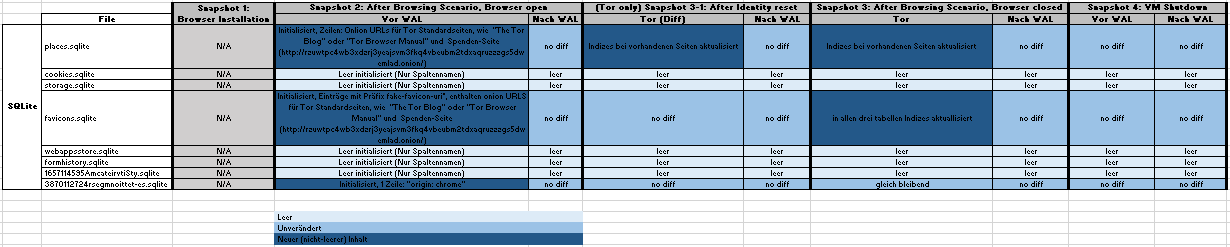
\includegraphics{bilder/tor-sqlite-table.png}}}
%	\label{chart:final-criteria}  
%	\caption{Comparison of found PB artifacts between RAM Dumps}
%\end{figure}

Nach Browser-Installation wurde noch keine SQLite-Datei angelegt (Snapshot 1).

Während des Browsing-Szenarios wurden alle Datenbanken initialisiert.
In places.sqlite wurden automatisch .onion-URLs geschrieben, die zu Tor Standardseiten führen. Beispielsweise Seiten wie \grqq{}The Tor Blog\grqq{} oder \grqq{}Tor Browser Manual\grqq{}.
Die gleichen Einträge wurden in der favicons.SQLite-Datenbank geschrieben, mit dem Präfix \grqq{}Fake-favicon-uri\grqq{}. Ein tatsächliches Icon wurde nicht in die Datenbank geschrieben. 
Weiterhin erhielt die \grqq{}remote settings\grqq{} Datenbank den gleichen Eintrag wie es bereits bei Firefox der Fall war. Der Eintrag enthält keine PB-Artefakte.
Die restliche SQLite-Dateien wurden ohne Inhalt angelegt, nur die Spaltennamen wurden definiert.
Nach Durchführung der WAL Checkpoints bleiben Dateien unverändert.

Nachdem dem Tor-Browser eine \grqq{}Neue Identität\grqq{} zugewiesen wurde (Snapshot 3-1), wurden in places.sqlite die Indizes bei den eingetragenen Seiten aktualisiert. Die restlichen Dateien blieben unverändert. Das Schreiben der WAL-Dateien in die Hauptdatenbanken veränderte den Inhalt nicht.

Nach Schließen des Browsers (Snapshot 3-2) wurden in places.sqlite sowie favicons.sqlite erneut Indizes bei eingetragenen Seiten aktualisiert. Die restliche Dateien blieben unverändert, ebenso ergaben die WAL Checkpoints keine Veränderungen.

Nach Herunterfahren der VM (Snapshot 4) blieben alle Datenbanken unverändert. Auch nach Durchführung der WAL Checkpoints gab es keine neuen Inhalte.

\subsubsection*{Zusammenfassung Tor Common Locations}
Im Balkendiagramm \ref{chart:firefox-writefile-logfile1v21vs22} ist zu erkennen, dass die meisten Schreiboperationen im ersten Logfile stattfinden. Dort werden Dateien jeder Kategorie beschrieben. Das Schließen des Tor-Browsers führt zu mehr oder genauso vielen Schreiboperationen wie das Zuweisen einer \grqq{}Neuen Identität\grqq{}. Keine der geschriebenen Dateien enthielt Private-Browsing-Artefakte.
%*** TODO: Was noch? ***
\begin{figure}[h!]
	\begin{tikzpicture}
	\begin{axis}[
	xbar, 
	xmin=0,
	width=12cm, 
	height=12cm, 
	xlabel={Anzahl Schreiboperationen},
	y=1.4cm,
	symbolic y coords={Sonstige Dateien,Datareporting,SQLite,Cache},
	ytick=data,
	xticklabels={,,},
	nodes near coords style={font=\small},
	nodes near coords={\pgfmathfloatifflags{\pgfplotspointmeta}{0}{}{\pgfmathprintnumber{\pgfplotspointmeta}}},
	bar width=.25cm,
	enlarge y limits={abs=2.4*\pgfplotbarwidth},
	legend style={
		at={(1,1)},
		anchor=north east
	},
	legend columns=2,
	scaled x ticks=false,
	yminorgrids = true,minor tick num=1
	]
	\addplot coordinates {(12,Sonstige Dateien) (2,Datareporting) (8,SQLite) (1,Cache)};
	\addplot coordinates {(3,Sonstige Dateien) (0,Datareporting) (1,SQLite) (0,Cache)};
	\addplot coordinates {(3,Sonstige Dateien) (1,Datareporting) (2,SQLite) (0,Cache)};	
	\legend{Logfile 1, Logfile 2-1, Logfile 2-2}
	\end{axis}
	\end{tikzpicture}
	\caption{Tor-Browser: Anzahl Schreiboperationen Logfile 1 vs Logfile 2-1 vs Logfile 2-2, geordnet nach Kategorie}
	\label{chart:firefox-writefile-logfile1v21vs22}
\end{figure}
%\begin{figure}[h!]
%	\centerline{\resizebox{\linewidth}{!}{\includegraphics{bilder/tor-bar-chart-logfile1vs2cs3.png}}}
%	\label{chart:final-criteria}  
%	\caption{Comparison of found PB artifacts between RAM Dumps}
%\end{figure}

%Literatur:
%	o no traces were found in “common locations” \cite{Montasari.2015}
%		>  “places.sqlite”, “webappsstore. sqlite”, “sessionstore.bak”, “search.json” and “nssckbi.dll”
%	o	Safebrowsing: Alle Dateien in /safebrowsing-updating/ nicht relevant. Dort nur .vlpset und .sbstore Dateien. Speichern 256-Bit Hash von URLs, die auf SafeSearch Blacklist stehen 
%	o	Cache-Dateien: drei Caches: startupCache, jumpListCache (beide enthalten Binärdateien ohne Browsing-Artefakte) und cache2 (können mit MZCacheView untersucht werden, enthalten keine Browsing-Artefakte)
%	o	SQLite-Datenbanken: Sqlite Dateien erst ohne WAL Dateien untersuchen, Danach mit sqlite3 Konsole: WAL in Datenbank schreiben mit: PRAGMA wal\_checkpoint; places.sqlite besonders relevant, da dort Browser in public Modus Browsing URLs verwaltet (Am besten hier vergleich mit Public Browsing machen)	
%		> \cite{Fayyad.2021} for Mozilla Firefox, 7 database files were recovered: cookies.sqlite-shm, places.sqlite-shm, prefs.js etc.
%		> \cite{Muir.2019} The two SQLite databases used by Firefox to track cookies and history (cookies.sqlite und places.sqlite) were both recoverable from the file system after deletion	
%		Ergebnisse stehen im Gegensatz zu \cite{Hedberg.2013} :
%			o	Chrome und Firefox: Einträge in places.sqlite + history.sqlite DB gefunden während PB! (Noch aktuell??)
%		Sonderfall: SQlite DB-Crash \cite{Hedberg.2013}
%			> WAL Files/Journal Files bei Crash gefunden -> Kann genutzt werden um zu beweisen, dass privater Browser genutzt wurde
%			> Daher: WAL Rollback mit sqlite3	
%	o	Jsonlz4 \& balkz4: Enthalten komprimierte Firefox-Sessions, jsonlz4 Dateien können mit Tool \grqq{}entkomprimiert\grqq{} werden: https://www.jeffersonscher.com/ffu/scrounger.html


\subsection{Uncommon Locations}
\label{subsection:appendix-tor-uncommon-locations}

\subsubsection*{Analyse mit Autopsy - Kategorisierte Dateien}
\label{subsubsection:appendix-tor-uncommon-locations-autopsy}

Wie bei Firefox in Kapitel \ref{subsubsection:appendix-firefox-uncommon-locations-autopsy} wurde keine der kategorisierten Dateien gelöscht. Somit befanden sich im letzten Festplatten-Image des Snapshots 4 alle kategorisierten Dateien der vorherigen Festplatten-Images

\paragraph*{Web Bookmarks}
Wie in Abbildung \ref{img:tor-web-bookmarks} gezeigt, wurden nur in der Datei \texttt{Bing.url} ein Lesezeichen zur Bing-Startseite gefunden. Diese Datei wurde im Festplatten-Image des ersten Snapshots geschrieben.
\begin{figure}[h!]
	\centerline{\resizebox{\linewidth}{!}{\includegraphics{bilder/cfv_tor_autopsy_web_bookmarks.png}}} 
	\caption{Tor-Browser: Von Autopsy als \grqq{}Web Bookmarks\grqq{} kategorisierte Dateien}
	\label{img:tor-web-bookmarks} 
\end{figure}

\paragraph*{Web Cookies}
Im Festplatte-Image des ersten VM-Snapshots wurden die in Abbildung \ref{img:tor-web-cookies} gezeigten neun Cookies-Einträge in die Datenbank des vorinstallierten Edge Browsers geschrieben. Dabei handelt es sich um Cookies für die Bing- und Outlook-Startseite.
\begin{figure}[h!]
	\centerline{\resizebox{\linewidth}{!}{\includegraphics{bilder/cfv_tor_autopsy_web_cookies.png}}} 
	\caption{Tor-Browser: Von Autopsy als \grqq{}Web Cookies\grqq{} kategorisierte Dateien}
	\label{img:tor-web-cookies} 
\end{figure}

\paragraph*{Web History}
Zwei Einträge mit Browsingverläufen wurden im Festplatten-Image des ersten VM-Snapshots in der Datei \texttt{WebCacheV01.dat} geschrieben. Wie in Abbildung \ref{img:tor-web-history} gezeigt, handelt es sich dabei zweimal um die Outlook-Startseite, obwohl diese nie bei der Versuchsdurchführung geöffnet wurde. Wie bei Firefox wurden in der Datei ebenfalls die zum Analyserechner über den gemeinsamen Ordner transportierten Process Monitor Logfiles gespeichert.
\begin{figure}[h!]
	\centerline{\resizebox{\linewidth}{!}{\includegraphics{bilder/cfv_tor_autopsy_web_history.png}}}
	\caption{Tor-Browser: Von Autopsy als \grqq{}Web History\grqq{} kategorisierte Dateien}
	\label{img:tor-web-history}  
\end{figure}

\paragraph*{Web Categories}
Autopsy klassifizierte im Festplatten-Image des ersten VM-Snapshots den Eintrag \texttt{bing.com} als \grqq{}Suchmaschine\grqq{}  und \texttt{live.com} als \grqq{}Web-Email\grqq{}, gezeigt in Abbildung \ref{img:tor-web-categories}.
Es gab keine zusätzlichen Einträge in dieser Kategorie in den Festplatten-Images der restlichen Snapshots.
\begin{figure}[h!]
	\centerline{\resizebox{\linewidth}{!}{\includegraphics{bilder/cfv_tor_autopsy_web_categories.png}}} 
	\caption{Tor-Browser: Von Autopsy als \grqq{}Web Categories\grqq{} kategorisierte Dateien}
	\label{img:tor-web-categories} 
\end{figure}
		
Somit wurden in den von Autopsy kategorisierten Dateien keine PB-Artefakte entdeckt. Weiterhin gab es verglichen mit der Analyse der Common Locations keine neuen Erkenntnisse. Autopsy erkannte nicht die in der places.sqlite-Datenbank geschriebenen .onion-URLs der Tor-Standardseiten.

%Literatur:
%	o	Autopsy Keywortsuche: 
%		>	In alles Snapshots ergebnislos (keine Keyword-Hits
%		-->	In Literatur: Autoren fanden Ergebnisse in pagefile.sys 
%			> Autopsy: websites and some of the keywords found in hidden file called “pagefile.sys” \cite{Mahlous.2020}
%			o \cite{Montasari.2015} traces were found in: 
%				> However, on investigating the “pagefile.sys”, some entries were discovered
%				> Using the “data carving” technique, profile picture was recovered
%			o \cite{Said.2011} 
%				> Examining pagefile.sys showed some positive hits 			
%		--> Evtl. hier zeigen, was gefunden werden kann, wenn RAM reduziert
%		--> Aber auf Problem hinweisen, dass gefundener String in pagefile nicht direkt Browser zugeordnet werden kann
%		> \cite{Gabet.2018}	Firefox only produced three recoverable artefacts as reported by both tools (FTK, Autopsy) --> Artefakte werden nicht genannt!
%		> \cite{Muir.2019} Autopsy Keyword Suche nach Suchbegriffen: unallocated space
%		> Autopsy Carving Module (\$Carved): \cite{Muir.2019}
%			•	When searching for the string ’clot’ from the browsing protocol, six .dll, .edb and .reg files were discovered in unallocated space.
%			•	Further searching of unallocated space uncovered references to the Tor installation directory and the obfs4 bridging IP addresses
%			•	browsing data found in NTUSER.DAT was also replicated in unallocated space.
%	o	Autopsy PlugIns:
%		>	*** TODO: Hier Liste mit PlugIns ***

\subsection{Registry}

\subsubsection*{Process Monitor SetValue Operations}

Bei Betrachtung als Common Locations werden gemäß Methodik in Abschnitt \ref{subsection:methodik-datenanalyse-registry} alle \grqq{}SetValue\grqq{} Schreiboperationen in den Process Monitor Logfiles für die Prozesse \grqq{}tor.exe\grqq{} und \grqq{}firefox.exe\grqq{} untersucht. 

Dabei wurden die gleichen beiden Registry Keys identifiziert, wie bei der Untersuchung der Firefox Registry in Kapitel \ref{subsubsection:appendix-firefox-registry-processmonitorsetvalue}: \texttt{PreXULSkeletonUISettings} und \texttt{Business Activity Monitoring}. In keinem Registry-Key befinden sich PB-Artefakte.
Wie in Abbildung \ref{chart:tor-registy-css-vs-bam} dargestellt, wurden beide Registry Keys annähernd gleich oft geschrieben. Bei Vergleich der drei Process Monitor Logfiles 1, 2 und 3 nimmt die Anzahl der Registry \grqq{}SetValue\grqq{}-Operationen bei Logfile 2 und 3 kontinuierlich ab.

\begin{figure}[h!]
	\resizebox{\linewidth}{!}{
	\begin{tikzpicture}
		\begin{axis}[
		xbar stacked,
		width=18cm, 
		height=12cm, 
%		ylabel style={align=center}, ylabel=RAM-Dump 1,
		y=1cm,
		enlarge y limits={abs=2*\pgfplotbarwidth},
		symbolic y coords={Logfile 2-2,Logfile 2-1,Logfile 1},
		ytick=data,
		xticklabels={,,},
        xmin = 0,
        xmax = 70,
		nodes near coords, 
		nodes near coords align={horizontal},
		legend style={
			at={(0.5,-0.1)},
			anchor=north
		},
		legend columns=2,
		scaled x ticks=false
		]
			\addplot coordinates {
			(10,Logfile 2-2) (14,Logfile 2-1) (27,Logfile 1)
			};
			\addplot coordinates {
			 (10,Logfile 2-2) (8,Logfile 2-1) (36,Logfile 1)
			};
			\legend{PreXULSkeletonUISettings (CSS), Business Activity Monitoring (BAM)}
		\end{axis}
	\end{tikzpicture}
	}	
	\caption{Tor-Browser: Registry \grqq{}SetValue\grqq{} Operationen in den Process Monitor Logfiles 1, 2-1 und 2-2}
	\label{chart:tor-registy-css-vs-bam}
\end{figure}

%\begin{figure}[h!]
%	\centerline{\resizebox{\linewidth}{!}{\includegraphics{bilder/tor-registry-stacked-bar-chart.png}}}
%	\label{chart:final-criteria}  
%	\caption{Comparison of found PB artifacts between RAM Dumps}
%\end{figure}

\subsubsection*{Stringsuche in Registry Hives}
Bei Betrachtung der Registry als Uncommon Locations, wurden die in Tabelle \ref{tab:windows-Registry Hives} in Abschnitt \ref{subsection:methodik-datenanalyse-registry} aufgelisteten Registry Hives mithilfe des Registry Explorers untersucht. 
Weder in den System-Hives noch in den User-Hives konnten PB-Artefakte identifiziert werden. 

%Literatur:
%	>	Auf Autor verweisen: angeblich in Shellactivities Ergebnisse. --> Nicht mehr vorhanden in aktueller Version (Verweis auf E-Mail)
%	>	Process Monitor/Regshot zeigen keine relevanten Key-Änderungen
%	> \cite{Muir.2019}: Autopsy Keyword Suche nach Suchbegriffen: Ergebnisse in \%SystemRoot\%Minidump NTUSER.DAT, ntuser.dat.LOG1 (a log of changes to NTUSER.DAT)
%	> Zentral: shellactivites Key:	NTUSER.DAT --> “shellactivities” key \cite{Muir.2019}
%	> \cite{Rochmadi.2017} Detection of registry changes helps to determine what the appropriate plugin is used to search for digital evidence using volatility memory forensic:
%	- RegQueryValue:	HKCU/Software/Microsoft/Windows/CurrentVersion/InternetSettings/Connections/DefaultConnectionSettings
%	- RegCloseValue: 	HKCU/Software/Microsoft/Windows/CurrentVersion/InternetSettings/Connections
%	- IRP\_MJ\_READ: C:/pagefile.sys

	
%		\addtocontents{toc}{\endgroup}

\pagebreak

\section{Ausführliche Analyse: Chrome}\label{chap:anhang-chrome}
\subsection{Common Locations}\label{chap:anhang-chrome-common-locations}
\subsubsection*{Process Monitor WriteFile Operations}\label{chap:anhang-chrome-common-locations-writefile-operations}

Gemäß Versuchsdurchführung wurden auch für Chrome 2 Logfiles erstellt, welche die Prozessaktivitäten während (Logfile 1) und nach dem Browsing Szenario während des Schließens des Browsers (Logfile 2) aufzeichnet. Beide Logfiles wurden gemäß Methodik in \autoref{subsection:methodik-datenanalyse-commonlocations} in Excel aufbereitet. \autoref{tab:chrome-writefile-operations} listet dabei alle Dateien auf, welche während des Szenarios durchgeführt wurden, \autoref{tab:chrome-writefile2-operations} hingegen alle Schreiboperationen beim Schließen des Browsers. Dabei wurde für jede Datei wieder vermerkt, ob und wie sie wiederherstellbar war, mit welchem Tool die Datei analysiert wurde und ob in der Datei PB Artefakte enthalten sind. Die Schreiboperationen wurden dieses mal in Dateiendungen gegliedert. In keiner der Dateien wurden PB Artefakte identifiziert.

Dabei wurde in \autoref{tab:chrome-writefile-operations} unterschieden zwischen den \textbf{Local}-Browser Pfaden (hellblau) und \textbf{andere Pfaden} (dunkelblau).\\
Zu sehen ist hier, dass hauptsächlich Dateien in den Browser-Pfad geschrieben werden.\\
Alle \textit{.tmp}-Dateien waren nicht wiederherstellbar, was eine Analyse unmöglich macht. Die Dateien mit dem Namen \textit{data\_1} waren jeweils vorhanden, enthielten jedoch keine PB Artefakte nach ausführlicher Analyse. Die \textit{-journal}-Dateien Diese sind sogenannte \glqq{}Rollback Journals\grqq{} und sind relevant für atomare Commit- und Rollback-Funktionen \cite{SQLiteTempfiles}. Da diese Dateien jedoch alle 0 Bytes groß waren, konnte hier kein Artefakt gefunden werden.\\
Auch wurden noch \textit{000003.log}-Dateien geschrieben. Diese sind Teil eines LevelDB-Schlüssel-\\wertespeichers \cite{LevelDBGithub,LevelDBCCL} . Mithife von HxD und einer Analyse mittels eines selbst erstellen Python-Scripts zur Ausgabe der Schlüssel-Werte-Paare derjenigen Ordner, welche die .log und weitere LevelDB spezifische Dateien enthalten, kann auch in diesen Ordner bzw. Dateien auch keine Artefakte gefunden werden.\\

\newgeometry{bottom=2cm,top=0.5cm}
%\setcounter{figure}{0}    
\afterpage{
\begin{landscape}% Landscape page
	\setcounter{page}{76}
%	\thispagestyle{empty}
	\vspace*{1.5cm}
	\hspace*{-1cm}
\begin{table}[h!]
%	\centering
	\caption{Chrome alle \grqq{}WriteFile\grqq{}-Operationen des Logfiles 1}
	\label{tab:chrome-writefile-operations}
	\vspace{0.5cm}
	\resizebox{\linewidth}{!}{
	\begin{tabular}{cllll}
		\multicolumn{5}{c}{\textbf{LOGFILE 1:}}                                                                                                                                                                                                                                                                                                                                                                                                                                                                                                                                                                                                                                                            \\ \hline
		\multicolumn{1}{|c|}{\textbf{Kategorie}}                                      & \multicolumn{1}{c|}{\textbf{Dateiname}}                                                                                                                                                                                                                                                                                                                                         & \multicolumn{1}{c|}{\textbf{Dateistatus}}                                                         & \multicolumn{1}{c|}{\textbf{Verwendetes Tool zur Analyse}} & \multicolumn{1}{l|}{\textbf{Enthaltene Artefakte}}              \\ \hline
		\multicolumn{1}{|c|}{}                                                        & \multicolumn{1}{l|}{\cellcolor[HTML]{34CDF9}C:\textbackslash{}Users\textbackslash{}Forensik\textbackslash{}AppData\textbackslash{}Local\textbackslash{}Google\textbackslash{}Chrome\textbackslash{}User   Data\textbackslash{}1f7ba833-406a-40cf-b107-6e391f4bd1d3.tmp}                                                                                                         & \multicolumn{1}{l|}{\cellcolor[HTML]{963400}{\color[HTML]{FFFFFF} Datei nicht wiederherstellbar}} & \multicolumn{1}{l|}{\cellcolor[HTML]{C0C0C0}N/A}           & \multicolumn{1}{l|}{\cellcolor[HTML]{C0C0C0}N/A}                \\ \cline{2-5} 
		\multicolumn{1}{|c|}{}                                                        & \multicolumn{1}{l|}{\cellcolor[HTML]{34CDF9}C:\textbackslash{}Users\textbackslash{}Forensik\textbackslash{}AppData\textbackslash{}Local\textbackslash{}Google\textbackslash{}Chrome\textbackslash{}User   Data\textbackslash{}2da074d0-9208-4026-b970-d7261bd389c3.tmp}                                                                                                         & \multicolumn{1}{l|}{\cellcolor[HTML]{963400}{\color[HTML]{FFFFFF} Datei nicht wiederherstellbar}} & \multicolumn{1}{l|}{\cellcolor[HTML]{C0C0C0}N/A}           & \multicolumn{1}{l|}{\cellcolor[HTML]{C0C0C0}N/A}                \\ \cline{2-5} 
		\multicolumn{1}{|c|}{}                                                        & \multicolumn{1}{l|}{\cellcolor[HTML]{34CDF9}C:\textbackslash{}Users\textbackslash{}Forensik\textbackslash{}AppData\textbackslash{}Local\textbackslash{}Google\textbackslash{}Chrome\textbackslash{}User   Data\textbackslash{}44a1b7b5-40eb-4265-8d3e-b55d21084e65.tmp}                                                                                                         & \multicolumn{1}{l|}{\cellcolor[HTML]{963400}{\color[HTML]{FFFFFF} Datei nicht wiederherstellbar}} & \multicolumn{1}{l|}{\cellcolor[HTML]{C0C0C0}N/A}           & \multicolumn{1}{l|}{\cellcolor[HTML]{C0C0C0}N/A}                \\ \cline{2-5} 
		\multicolumn{1}{|c|}{}                                                        & \multicolumn{1}{l|}{\cellcolor[HTML]{34CDF9}C:\textbackslash{}Users\textbackslash{}Forensik\textbackslash{}AppData\textbackslash{}Local\textbackslash{}Google\textbackslash{}Chrome\textbackslash{}User   Data\textbackslash{}6f9e2d84-9a77-41e3-8955-b0c836f8fd0c.tmp}                                                                                                         & \multicolumn{1}{l|}{\cellcolor[HTML]{963400}{\color[HTML]{FFFFFF} Datei nicht wiederherstellbar}} & \multicolumn{1}{l|}{\cellcolor[HTML]{C0C0C0}N/A}           & \multicolumn{1}{l|}{\cellcolor[HTML]{C0C0C0}N/A}                \\ \cline{2-5} 
		\multicolumn{1}{|c|}{}                                                        & \multicolumn{1}{l|}{\cellcolor[HTML]{34CDF9}C:\textbackslash{}Users\textbackslash{}Forensik\textbackslash{}AppData\textbackslash{}Local\textbackslash{}Google\textbackslash{}Chrome\textbackslash{}User   Data\textbackslash{}8b2096fb-9e68-4a4c-9df5-3dd0949aa210.tmp}                                                                                                         & \multicolumn{1}{l|}{\cellcolor[HTML]{963400}{\color[HTML]{FFFFFF} Datei nicht wiederherstellbar}} & \multicolumn{1}{l|}{\cellcolor[HTML]{C0C0C0}N/A}           & \multicolumn{1}{l|}{\cellcolor[HTML]{C0C0C0}N/A}                \\ \cline{2-5} 
		\multicolumn{1}{|c|}{}                                                        & \multicolumn{1}{l|}{\cellcolor[HTML]{34CDF9}C:\textbackslash{}Users\textbackslash{}Forensik\textbackslash{}AppData\textbackslash{}Local\textbackslash{}Google\textbackslash{}Chrome\textbackslash{}User   Data\textbackslash{}97615fa9-9081-43b0-af51-534da2fd8cb4.tmp}                                                                                                         & \multicolumn{1}{l|}{\cellcolor[HTML]{963400}{\color[HTML]{FFFFFF} Datei nicht wiederherstellbar}} & \multicolumn{1}{l|}{\cellcolor[HTML]{C0C0C0}N/A}           & \multicolumn{1}{l|}{\cellcolor[HTML]{C0C0C0}N/A}                \\ \cline{2-5} 
		\multicolumn{1}{|c|}{}                                                        & \multicolumn{1}{l|}{\cellcolor[HTML]{34CDF9}C:\textbackslash{}Users\textbackslash{}Forensik\textbackslash{}AppData\textbackslash{}Local\textbackslash{}Google\textbackslash{}Chrome\textbackslash{}User   Data\textbackslash{}a0ea17f1-38e8-48e0-a2f4-98e9be6a6dd3.tmp}                                                                                                         & \multicolumn{1}{l|}{\cellcolor[HTML]{963400}{\color[HTML]{FFFFFF} Datei nicht wiederherstellbar}} & \multicolumn{1}{l|}{\cellcolor[HTML]{C0C0C0}N/A}           & \multicolumn{1}{l|}{\cellcolor[HTML]{C0C0C0}N/A}                \\ \cline{2-5} 
		\multicolumn{1}{|c|}{}                                                        & \multicolumn{1}{l|}{\cellcolor[HTML]{34CDF9}C:\textbackslash{}Users\textbackslash{}Forensik\textbackslash{}AppData\textbackslash{}Local\textbackslash{}Google\textbackslash{}Chrome\textbackslash{}User   Data\textbackslash{}b23e8f25-4bfb-4625-a9d5-836ff096b671.tmp}                                                                                                         & \multicolumn{1}{l|}{\cellcolor[HTML]{963400}{\color[HTML]{FFFFFF} Datei nicht wiederherstellbar}} & \multicolumn{1}{l|}{\cellcolor[HTML]{C0C0C0}N/A}           & \multicolumn{1}{l|}{\cellcolor[HTML]{C0C0C0}N/A}                \\ \cline{2-5} 
		\multicolumn{1}{|c|}{}                                                        & \multicolumn{1}{l|}{\cellcolor[HTML]{34CDF9}C:\textbackslash{}Users\textbackslash{}Forensik\textbackslash{}AppData\textbackslash{}Local\textbackslash{}Google\textbackslash{}Chrome\textbackslash{}User   Data\textbackslash{}c029e5f2-88df-4271-bc24-2c50db41cc89.tmp}                                                                                                         & \multicolumn{1}{l|}{\cellcolor[HTML]{963400}{\color[HTML]{FFFFFF} Datei nicht wiederherstellbar}} & \multicolumn{1}{l|}{\cellcolor[HTML]{C0C0C0}N/A}           & \multicolumn{1}{l|}{\cellcolor[HTML]{C0C0C0}N/A}                \\ \cline{2-5} 
		\multicolumn{1}{|c|}{}                                                        & \multicolumn{1}{l|}{\cellcolor[HTML]{34CDF9}C:\textbackslash{}Users\textbackslash{}Forensik\textbackslash{}AppData\textbackslash{}Local\textbackslash{}Google\textbackslash{}Chrome\textbackslash{}User   Data\textbackslash{}Default\textbackslash{}9a105eba-925a-4d38-994f-c59962a8a60c.tmp}                                                                                  & \multicolumn{1}{l|}{\cellcolor[HTML]{963400}{\color[HTML]{FFFFFF} Datei nicht wiederherstellbar}} & \multicolumn{1}{l|}{\cellcolor[HTML]{C0C0C0}N/A}           & \multicolumn{1}{l|}{\cellcolor[HTML]{C0C0C0}N/A}                \\ \cline{2-5} 
		\multicolumn{1}{|c|}{}                                                        & \multicolumn{1}{l|}{\cellcolor[HTML]{34CDF9}C:\textbackslash{}Users\textbackslash{}Forensik\textbackslash{}AppData\textbackslash{}Local\textbackslash{}Google\textbackslash{}Chrome\textbackslash{}User   Data\textbackslash{}Default\textbackslash{}Network\textbackslash{}184cc287-bc19-4faf-bd09-fdfc1ff1c6b8.tmp}                                                           & \multicolumn{1}{l|}{\cellcolor[HTML]{963400}{\color[HTML]{FFFFFF} Datei nicht wiederherstellbar}} & \multicolumn{1}{l|}{\cellcolor[HTML]{C0C0C0}N/A}           & \multicolumn{1}{l|}{\cellcolor[HTML]{C0C0C0}N/A}                \\ \cline{2-5} 
		\multicolumn{1}{|c|}{}                                                        & \multicolumn{1}{l|}{\cellcolor[HTML]{34CDF9}C:\textbackslash{}Users\textbackslash{}Forensik\textbackslash{}AppData\textbackslash{}Local\textbackslash{}Google\textbackslash{}Chrome\textbackslash{}User   Data\textbackslash{}Default\textbackslash{}Network\textbackslash{}a3ab3887-9ed6-45e7-a1bc-e0a34974b332.tmp}                                                           & \multicolumn{1}{l|}{\cellcolor[HTML]{963400}{\color[HTML]{FFFFFF} Datei nicht wiederherstellbar}} & \multicolumn{1}{l|}{\cellcolor[HTML]{C0C0C0}N/A}           & \multicolumn{1}{l|}{\cellcolor[HTML]{C0C0C0}N/A}                \\ \cline{2-5} 
		\multicolumn{1}{|c|}{}                                                        & \multicolumn{1}{l|}{\cellcolor[HTML]{34CDF9}C:\textbackslash{}Users\textbackslash{}Forensik\textbackslash{}AppData\textbackslash{}Local\textbackslash{}Google\textbackslash{}Chrome\textbackslash{}User   Data\textbackslash{}e5e0606b-51a1-44ba-a8f9-80f1cf5c48a3.tmp}                                                                                                         & \multicolumn{1}{l|}{\cellcolor[HTML]{963400}{\color[HTML]{FFFFFF} Datei nicht wiederherstellbar}} & \multicolumn{1}{l|}{\cellcolor[HTML]{C0C0C0}N/A}           & \multicolumn{1}{l|}{\cellcolor[HTML]{C0C0C0}N/A}                \\ \cline{2-5} 
		\multicolumn{1}{|c|}{}                                                        & \multicolumn{1}{l|}{\cellcolor[HTML]{34CDF9}C:\textbackslash{}Users\textbackslash{}Forensik\textbackslash{}AppData\textbackslash{}Local\textbackslash{}Google\textbackslash{}Chrome\textbackslash{}User   Data\textbackslash{}fbd23442-8e9b-47cb-95e6-9da65df2c42e.tmp}                                                                                                         & \multicolumn{1}{l|}{\cellcolor[HTML]{963400}{\color[HTML]{FFFFFF} Datei nicht wiederherstellbar}} & \multicolumn{1}{l|}{\cellcolor[HTML]{C0C0C0}N/A}           & \multicolumn{1}{l|}{\cellcolor[HTML]{C0C0C0}N/A}                \\ \cline{2-5} 
		\multicolumn{1}{|c|}{\multirow{-15}{*}{\textit{Temp files (.tmp)}}}           & \multicolumn{1}{l|}{\cellcolor[HTML]{34CDF9}C:\textbackslash{}Users\textbackslash{}Forensik\textbackslash{}AppData\textbackslash{}Local\textbackslash{}Google\textbackslash{}Chrome\textbackslash{}User   Data\textbackslash{}fecad46f-9d32-40a2-aa3c-7b1cc275a5e2.tmp}                                                                                                         & \multicolumn{1}{l|}{\cellcolor[HTML]{963400}{\color[HTML]{FFFFFF} Datei nicht wiederherstellbar}} & \multicolumn{1}{l|}{\cellcolor[HTML]{C0C0C0}N/A}           & \multicolumn{1}{l|}{\cellcolor[HTML]{C0C0C0}N/A}                \\ \hline
		\multicolumn{1}{|c|}{}                                                        & \multicolumn{1}{l|}{\cellcolor[HTML]{34CDF9}C:\textbackslash{}Users\textbackslash{}Forensik\textbackslash{}AppData\textbackslash{}Local\textbackslash{}Google\textbackslash{}Chrome\textbackslash{}User   Data\textbackslash{}Default\textbackslash{}Cache\textbackslash{}Cache\_Data\textbackslash{}data\_1}                                                                   & \multicolumn{1}{l|}{\cellcolor[HTML]{009901}Datei vorhanden}                                      & \multicolumn{1}{l|}{ChromeCacheView}                       & \multicolumn{1}{l|}{\cellcolor[HTML]{F8A102}Keine PB Artefakte} \\ \cline{2-5} 
		\multicolumn{1}{|c|}{}                                                        & \multicolumn{1}{l|}{\cellcolor[HTML]{34CDF9}C:\textbackslash{}Users\textbackslash{}Forensik\textbackslash{}AppData\textbackslash{}Local\textbackslash{}Google\textbackslash{}Chrome\textbackslash{}User   Data\textbackslash{}Default\textbackslash{}DawnCache\textbackslash{}data\_1}                                                                                          & \multicolumn{1}{l|}{\cellcolor[HTML]{009901}Datei vorhanden}                                      & \multicolumn{1}{l|}{HxD}                                   & \multicolumn{1}{l|}{\cellcolor[HTML]{F8A102}Keine PB Artefakte} \\ \cline{2-5} 
		\multicolumn{1}{|c|}{}                                                        & \multicolumn{1}{l|}{\cellcolor[HTML]{34CDF9}C:\textbackslash{}Users\textbackslash{}Forensik\textbackslash{}AppData\textbackslash{}Local\textbackslash{}Google\textbackslash{}Chrome\textbackslash{}User   Data\textbackslash{}Default\textbackslash{}GPUCache\textbackslash{}data\_1}                                                                                           & \multicolumn{1}{l|}{\cellcolor[HTML]{009901}Datei vorhanden}                                      & \multicolumn{1}{l|}{HxD}                                   & \multicolumn{1}{l|}{\cellcolor[HTML]{F8A102}Keine PB Artefakte} \\ \cline{2-5} 
		\multicolumn{1}{|c|}{}                                                        & \multicolumn{1}{l|}{\cellcolor[HTML]{34CDF9}C:\textbackslash{}Users\textbackslash{}Forensik\textbackslash{}AppData\textbackslash{}Local\textbackslash{}Google\textbackslash{}Chrome\textbackslash{}User   Data\textbackslash{}GrShaderCache\textbackslash{}data\_1}                                                                                                             & \multicolumn{1}{l|}{\cellcolor[HTML]{009901}Datei vorhanden}                                      & \multicolumn{1}{l|}{HxD}                                   & \multicolumn{1}{l|}{\cellcolor[HTML]{F8A102}Keine PB Artefakte} \\ \cline{2-5} 
		\multicolumn{1}{|c|}{\multirow{-5}{*}{\textit{data\_1 files}}}                & \multicolumn{1}{l|}{\cellcolor[HTML]{34CDF9}C:\textbackslash{}Users\textbackslash{}Forensik\textbackslash{}AppData\textbackslash{}Local\textbackslash{}Google\textbackslash{}Chrome\textbackslash{}User   Data\textbackslash{}ShaderCache\textbackslash{}data\_1}                                                                                                               & \multicolumn{1}{l|}{\cellcolor[HTML]{009901}Datei vorhanden}                                      & \multicolumn{1}{l|}{HxD}                                   & \multicolumn{1}{l|}{\cellcolor[HTML]{F8A102}Keine PB Artefakte} \\ \hline
		\multicolumn{1}{|c|}{}                                                        & \multicolumn{1}{l|}{\cellcolor[HTML]{34CDF9}C:\textbackslash{}Users\textbackslash{}Forensik\textbackslash{}AppData\textbackslash{}Local\textbackslash{}Google\textbackslash{}Chrome\textbackslash{}User   Data\textbackslash{}Default\textbackslash{}History-journal}                                                                                                           & \multicolumn{1}{l|}{\cellcolor[HTML]{AB70E9}Datei leer (0 Bytes groß)}                            & \multicolumn{1}{l|}{\cellcolor[HTML]{C0C0C0}N/A}           & \multicolumn{1}{l|}{\cellcolor[HTML]{C0C0C0}N/A}                \\ \cline{2-5} 
		\multicolumn{1}{|c|}{}                                                        & \multicolumn{1}{l|}{\cellcolor[HTML]{34CDF9}C:\textbackslash{}Users\textbackslash{}Forensik\textbackslash{}AppData\textbackslash{}Local\textbackslash{}Google\textbackslash{}Chrome\textbackslash{}User   Data\textbackslash{}Default\textbackslash{}Network\textbackslash{}Reporting and NEL-journal}                                                                          & \multicolumn{1}{l|}{\cellcolor[HTML]{AB70E9}Datei leer (0 Bytes groß)}                            & \multicolumn{1}{l|}{\cellcolor[HTML]{C0C0C0}N/A}           & \multicolumn{1}{l|}{\cellcolor[HTML]{C0C0C0}N/A}                \\ \cline{2-5} 
		\multicolumn{1}{|c|}{\multirow{-3}{*}{\textit{SQLite -journal Dateien}}}      & \multicolumn{1}{l|}{\cellcolor[HTML]{34CDF9}C:\textbackslash{}Users\textbackslash{}Forensik\textbackslash{}AppData\textbackslash{}Local\textbackslash{}Google\textbackslash{}Chrome\textbackslash{}User   Data\textbackslash{}Default\textbackslash{}Web Data-journal}                                                                                                          & \multicolumn{1}{l|}{\cellcolor[HTML]{AB70E9}Datei leer (0 Bytes groß)}                            & \multicolumn{1}{l|}{\cellcolor[HTML]{C0C0C0}N/A}           & \multicolumn{1}{l|}{\cellcolor[HTML]{C0C0C0}N/A}                \\ \hline
		\multicolumn{1}{|c|}{}                                                        & \multicolumn{1}{l|}{\cellcolor[HTML]{34CDF9}C:\textbackslash{}Users\textbackslash{}Forensik\textbackslash{}AppData\textbackslash{}Local\textbackslash{}Google\textbackslash{}Chrome\textbackslash{}User   Data\textbackslash{}Default\textbackslash{}shared\_proto\_db\textbackslash{}000003.log}                                                                               & \multicolumn{1}{l|}{\cellcolor[HTML]{009901}Datei vorhanden}                                      & \multicolumn{1}{l|}{HxD}                                   & \multicolumn{1}{l|}{\cellcolor[HTML]{F8A102}Keine PB Artefakte} \\ \cline{2-5} 
		\multicolumn{1}{|c|}{\multirow{-2}{*}{\textit{000003.log Dateien (LevelDB)}}} & \multicolumn{1}{l|}{\cellcolor[HTML]{34CDF9}C:\textbackslash{}Users\textbackslash{}Forensik\textbackslash{}AppData\textbackslash{}Local\textbackslash{}Google\textbackslash{}Chrome\textbackslash{}User   Data\textbackslash{}Default\textbackslash{}Sync Data\textbackslash{}LevelDB\textbackslash{}000003.log}                                                                & \multicolumn{1}{l|}{\cellcolor[HTML]{009901}Datei vorhanden}                                      & \multicolumn{1}{l|}{HxD}                                   & \multicolumn{1}{l|}{\cellcolor[HTML]{F8A102}Keine PB Artefakte} \\ \hline
		\multicolumn{1}{|c|}{}                                                        & \multicolumn{1}{l|}{\cellcolor[HTML]{34CDF9}C:\textbackslash{}Users\textbackslash{}Forensik\textbackslash{}AppData\textbackslash{}Local\textbackslash{}Google\textbackslash{}Chrome\textbackslash{}User   Data\textbackslash{}Default\textbackslash{}Web Applications\textbackslash{}Temp\textbackslash{}scoped\_dir764\_530297989\textbackslash{}Icons\textbackslash{}128.png} & \multicolumn{1}{l|}{\cellcolor[HTML]{963400}{\color[HTML]{FFFFFF} Datei nicht wiederherstellbar}} & \multicolumn{1}{l|}{\cellcolor[HTML]{C0C0C0}N/A}           & \multicolumn{1}{l|}{\cellcolor[HTML]{C0C0C0}N/A}                \\ \cline{2-5} 
		\multicolumn{1}{|c|}{}                                                        & \multicolumn{1}{l|}{\cellcolor[HTML]{34CDF9}C:\textbackslash{}Users\textbackslash{}Forensik\textbackslash{}AppData\textbackslash{}Local\textbackslash{}Google\textbackslash{}Chrome\textbackslash{}User   Data\textbackslash{}Default\textbackslash{}Web Applications\textbackslash{}Temp\textbackslash{}scoped\_dir764\_530297989\textbackslash{}Icons\textbackslash{}192.png} & \multicolumn{1}{l|}{\cellcolor[HTML]{963400}{\color[HTML]{FFFFFF} Datei nicht wiederherstellbar}} & \multicolumn{1}{l|}{\cellcolor[HTML]{C0C0C0}N/A}           & \multicolumn{1}{l|}{\cellcolor[HTML]{C0C0C0}N/A}                \\ \cline{2-5} 
		\multicolumn{1}{|c|}{}                                                        & \multicolumn{1}{l|}{\cellcolor[HTML]{34CDF9}C:\textbackslash{}Users\textbackslash{}Forensik\textbackslash{}AppData\textbackslash{}Local\textbackslash{}Google\textbackslash{}Chrome\textbackslash{}User   Data\textbackslash{}Default\textbackslash{}Web Applications\textbackslash{}Temp\textbackslash{}scoped\_dir764\_530297989\textbackslash{}Icons\textbackslash{}256.png} & \multicolumn{1}{l|}{\cellcolor[HTML]{963400}{\color[HTML]{FFFFFF} Datei nicht wiederherstellbar}} & \multicolumn{1}{l|}{\cellcolor[HTML]{C0C0C0}N/A}           & \multicolumn{1}{l|}{\cellcolor[HTML]{C0C0C0}N/A}                \\ \cline{2-5} 
		\multicolumn{1}{|c|}{}                                                        & \multicolumn{1}{l|}{\cellcolor[HTML]{34CDF9}C:\textbackslash{}Users\textbackslash{}Forensik\textbackslash{}AppData\textbackslash{}Local\textbackslash{}Google\textbackslash{}Chrome\textbackslash{}User   Data\textbackslash{}Default\textbackslash{}Web Applications\textbackslash{}Temp\textbackslash{}scoped\_dir764\_530297989\textbackslash{}Icons\textbackslash{}32.png}  & \multicolumn{1}{l|}{\cellcolor[HTML]{963400}{\color[HTML]{FFFFFF} Datei nicht wiederherstellbar}} & \multicolumn{1}{l|}{\cellcolor[HTML]{C0C0C0}N/A}           & \multicolumn{1}{l|}{\cellcolor[HTML]{C0C0C0}N/A}                \\ \cline{2-5} 
		\multicolumn{1}{|c|}{}                                                        & \multicolumn{1}{l|}{\cellcolor[HTML]{34CDF9}C:\textbackslash{}Users\textbackslash{}Forensik\textbackslash{}AppData\textbackslash{}Local\textbackslash{}Google\textbackslash{}Chrome\textbackslash{}User   Data\textbackslash{}Default\textbackslash{}Web Applications\textbackslash{}Temp\textbackslash{}scoped\_dir764\_530297989\textbackslash{}Icons\textbackslash{}48.png}  & \multicolumn{1}{l|}{\cellcolor[HTML]{963400}{\color[HTML]{FFFFFF} Datei nicht wiederherstellbar}} & \multicolumn{1}{l|}{\cellcolor[HTML]{C0C0C0}N/A}           & \multicolumn{1}{l|}{\cellcolor[HTML]{C0C0C0}N/A}                \\ \cline{2-5} 
		\multicolumn{1}{|c|}{}                                                        & \multicolumn{1}{l|}{\cellcolor[HTML]{34CDF9}C:\textbackslash{}Users\textbackslash{}Forensik\textbackslash{}AppData\textbackslash{}Local\textbackslash{}Google\textbackslash{}Chrome\textbackslash{}User   Data\textbackslash{}Default\textbackslash{}Web Applications\textbackslash{}Temp\textbackslash{}scoped\_dir764\_530297989\textbackslash{}Icons\textbackslash{}512.png} & \multicolumn{1}{l|}{\cellcolor[HTML]{963400}{\color[HTML]{FFFFFF} Datei nicht wiederherstellbar}} & \multicolumn{1}{l|}{\cellcolor[HTML]{C0C0C0}N/A}           & \multicolumn{1}{l|}{\cellcolor[HTML]{C0C0C0}N/A}                \\ \cline{2-5} 
		\multicolumn{1}{|c|}{}                                                        & \multicolumn{1}{l|}{\cellcolor[HTML]{34CDF9}C:\textbackslash{}Users\textbackslash{}Forensik\textbackslash{}AppData\textbackslash{}Local\textbackslash{}Google\textbackslash{}Chrome\textbackslash{}User   Data\textbackslash{}Default\textbackslash{}Web Applications\textbackslash{}Temp\textbackslash{}scoped\_dir764\_530297989\textbackslash{}Icons\textbackslash{}64.png}  & \multicolumn{1}{l|}{\cellcolor[HTML]{963400}{\color[HTML]{FFFFFF} Datei nicht wiederherstellbar}} & \multicolumn{1}{l|}{\cellcolor[HTML]{C0C0C0}N/A}           & \multicolumn{1}{l|}{\cellcolor[HTML]{C0C0C0}N/A}                \\ \cline{2-5} 
		\multicolumn{1}{|c|}{\multirow{-8}{*}{\textit{Temporary .png files}}}         & \multicolumn{1}{l|}{\cellcolor[HTML]{34CDF9}C:\textbackslash{}Users\textbackslash{}Forensik\textbackslash{}AppData\textbackslash{}Local\textbackslash{}Google\textbackslash{}Chrome\textbackslash{}User   Data\textbackslash{}Default\textbackslash{}Web Applications\textbackslash{}Temp\textbackslash{}scoped\_dir764\_530297989\textbackslash{}Icons\textbackslash{}96.png}  & \multicolumn{1}{l|}{\cellcolor[HTML]{963400}{\color[HTML]{FFFFFF} Datei nicht wiederherstellbar}} & \multicolumn{1}{l|}{\cellcolor[HTML]{C0C0C0}N/A}           & \multicolumn{1}{l|}{\cellcolor[HTML]{C0C0C0}N/A}                \\ \hline
		\multicolumn{1}{|c|}{}                                                        & \multicolumn{1}{l|}{\cellcolor[HTML]{3190FF}C:\textbackslash{}Users\textbackslash{}Forensik\textbackslash{}AppData\textbackslash{}Roaming\textbackslash{}Microsoft\textbackslash{}Spelling\textbackslash{}de-DE\textbackslash{}default.acl}                                                                                                                                     & \multicolumn{1}{l|}{\cellcolor[HTML]{009901}Datei vorhanden}                                      & \multicolumn{1}{l|}{HxD}                                   & \multicolumn{1}{l|}{\cellcolor[HTML]{F8A102}Keine PB Artefakte} \\ \cline{2-5} 
		\multicolumn{1}{|c|}{}                                                        & \multicolumn{1}{l|}{\cellcolor[HTML]{3190FF}C:\textbackslash{}Users\textbackslash{}Forensik\textbackslash{}AppData\textbackslash{}Roaming\textbackslash{}Microsoft\textbackslash{}Spelling\textbackslash{}de-DE\textbackslash{}default.dic}                                                                                                                                     & \multicolumn{1}{l|}{\cellcolor[HTML]{009901}Datei vorhanden}                                      & \multicolumn{1}{l|}{HxD}                                   & \multicolumn{1}{l|}{\cellcolor[HTML]{F8A102}Keine PB Artefakte} \\ \cline{2-5} 
		\multicolumn{1}{|c|}{\multirow{-3}{*}{\textit{Spelling default files}}}       & \multicolumn{1}{l|}{\cellcolor[HTML]{3190FF}C:\textbackslash{}Users\textbackslash{}Forensik\textbackslash{}AppData\textbackslash{}Roaming\textbackslash{}Microsoft\textbackslash{}Spelling\textbackslash{}de-DE\textbackslash{}default.exc}                                                                                                                                     & \multicolumn{1}{l|}{\cellcolor[HTML]{009901}Datei vorhanden}                                      & \multicolumn{1}{l|}{HxD}                                   & \multicolumn{1}{l|}{\cellcolor[HTML]{F8A102}Keine PB Artefakte} \\ \hline
		\multicolumn{1}{|c|}{}                                                        & \multicolumn{1}{l|}{\cellcolor[HTML]{3190FF}C:\textbackslash{}Users\textbackslash{}Forensik\textbackslash{}AppData\textbackslash{}Local\textbackslash{}D3DSCache\textbackslash{}cb00da9ba77862e\textbackslash{}F4EB2D6C-ED2B-4BDD-AD9D-F913287E6768.idx}                                                                                                                        & \multicolumn{1}{l|}{\cellcolor[HTML]{009901}Datei vorhanden}                                      & \multicolumn{1}{l|}{HxD}                                   & \multicolumn{1}{l|}{\cellcolor[HTML]{F8A102}Keine PB Artefakte} \\ \cline{2-5} 
		\multicolumn{1}{|c|}{}                                                        & \multicolumn{1}{l|}{\cellcolor[HTML]{3190FF}C:\textbackslash{}Users\textbackslash{}Forensik\textbackslash{}AppData\textbackslash{}Local\textbackslash{}D3DSCache\textbackslash{}cb00da9ba77862e\textbackslash{}F4EB2D6C-ED2B-4BDD-AD9D-F913287E6768.lock}                                                                                                                       & \multicolumn{1}{l|}{\cellcolor[HTML]{009901}Datei vorhanden}                                      & \multicolumn{1}{l|}{HxD}                                   & \multicolumn{1}{l|}{\cellcolor[HTML]{F8A102}Keine PB Artefakte} \\ \cline{2-5} 
		\multicolumn{1}{|c|}{\multirow{-3}{*}{\textit{D3DS Cache}}}                   & \multicolumn{1}{l|}{\cellcolor[HTML]{3190FF}C:\textbackslash{}Users\textbackslash{}Forensik\textbackslash{}AppData\textbackslash{}Local\textbackslash{}D3DSCache\textbackslash{}cb00da9ba77862e\textbackslash{}F4EB2D6C-ED2B-4BDD-AD9D-F913287E6768.val}                                                                                                                        & \multicolumn{1}{l|}{\cellcolor[HTML]{009901}Datei vorhanden}                                      & \multicolumn{1}{l|}{HxD}                                   & \multicolumn{1}{l|}{\cellcolor[HTML]{F8A102}Keine PB Artefakte} \\ \hline
		\multicolumn{1}{l}{}                                                          &                                                                                                                                                                                                                                                                                                                                                                                 &                                                                                                   &                                                            &                                                                 \\
		\multicolumn{1}{l}{}                                                          &                                                                                                                                                                                                                                                                                                                                                                                 &                                                                                                   &                                                            &                                                                 \\
		\multicolumn{1}{l}{}                                                          &                                                                                                                                                                                                                                                                                                                                                                                 &                                                                                                   &                                                            &                                                                
	\end{tabular}
}
\end{table}
\end{landscape}
%}
%\restoregeometry

%\newgeometry{bottom=2cm,top=0.5cm}
%\setcounter{figure}{0}    
%\afterpage{
	\begin{landscape}% Landscape page
		%\setcounter{page}{60}
		%	\thispagestyle{empty}
		\vspace*{1.5cm}
		\hspace*{-1cm}
		\begin{table}[h!]
			%	\centering
			\caption{Chrome: alle \grqq{}WriteFile\grqq{}-Operationen des Logfiles 2}
			\label{tab:chrome-writefile2-operations}
			\vspace{0.5cm}
			\resizebox{\linewidth}{!}{
				\begin{tabular}{cllll}
					\multicolumn{5}{c}{\textbf{LOGFILE 2:}}                                                                                                                                                                                                                                                                                                                                                                                                                                                                                                                                                                                                                                                                                                    \\ \hline
					\multicolumn{1}{|c|}{\textbf{Kategorie}}                           & \multicolumn{1}{c|}{\textbf{Dateiname}}                                                                                                                                                                                                                                                                                                                                                                                            & \multicolumn{1}{c|}{\textbf{Dateistatus}}                                                         & \multicolumn{1}{c|}{\textbf{Verwendetes Tool zur Analyse}} & \multicolumn{1}{l|}{\textbf{Enthaltene Artefakte}}              \\ \hline
					\multicolumn{1}{|c|}{\textit{settings.dat}}                        & \multicolumn{1}{l|}{\cellcolor[HTML]{34CDF9}C:\textbackslash{}Users\textbackslash{}Forensik\textbackslash{}AppData\textbackslash{}Local\textbackslash{}Google\textbackslash{}Chrome\textbackslash{}User   Data\textbackslash{}Crashpad\textbackslash{}settings.dat}                                                                                                                                                                & \multicolumn{1}{l|}{\cellcolor[HTML]{009901}{\color[HTML]{FFFFFF} Datei vorhanden}}               & \multicolumn{1}{l|}{HxD}                                   & \multicolumn{1}{l|}{\cellcolor[HTML]{F8A102}Keine PB Artefakte} \\ \hline
					\multicolumn{1}{|c|}{}                                             & \multicolumn{1}{l|}{\cellcolor[HTML]{34CDF9}C:\textbackslash{}Users\textbackslash{}Forensik\textbackslash{}AppData\textbackslash{}Local\textbackslash{}Google\textbackslash{}Chrome\textbackslash{}User   Data\textbackslash{}35debf2e-9a97-4829-b0d1-2c6efb7246bc.tmp}                                                                                                                                                            & \multicolumn{1}{l|}{\cellcolor[HTML]{963400}{\color[HTML]{FFFFFF} Datei nicht wiederherstellbar}} & \multicolumn{1}{l|}{\cellcolor[HTML]{C0C0C0}N/A}           & \multicolumn{1}{l|}{\cellcolor[HTML]{C0C0C0}N/A}                \\ \cline{2-5} 
					\multicolumn{1}{|c|}{}                                             & \multicolumn{1}{l|}{\cellcolor[HTML]{34CDF9}C:\textbackslash{}Users\textbackslash{}Forensik\textbackslash{}AppData\textbackslash{}Local\textbackslash{}Google\textbackslash{}Chrome\textbackslash{}User   Data\textbackslash{}4dce7d9d-2753-424d-ad13-eb84e1ea9326.tmp}                                                                                                                                                            & \multicolumn{1}{l|}{\cellcolor[HTML]{963400}{\color[HTML]{FFFFFF} Datei nicht wiederherstellbar}} & \multicolumn{1}{l|}{\cellcolor[HTML]{C0C0C0}N/A}           & \multicolumn{1}{l|}{\cellcolor[HTML]{C0C0C0}N/A}                \\ \cline{2-5} 
					\multicolumn{1}{|c|}{}                                             & \multicolumn{1}{l|}{\cellcolor[HTML]{34CDF9}C:\textbackslash{}Users\textbackslash{}Forensik\textbackslash{}AppData\textbackslash{}Local\textbackslash{}Google\textbackslash{}Chrome\textbackslash{}User   Data\textbackslash{}Default\textbackslash{}51ff0ac1-e188-4c8a-8b3d-891f326bb890.tmp}                                                                                                                                     & \multicolumn{1}{l|}{\cellcolor[HTML]{963400}{\color[HTML]{FFFFFF} Datei nicht wiederherstellbar}} & \multicolumn{1}{l|}{\cellcolor[HTML]{C0C0C0}N/A}           & \multicolumn{1}{l|}{\cellcolor[HTML]{C0C0C0}N/A}                \\ \cline{2-5} 
					\multicolumn{1}{|c|}{}                                             & \multicolumn{1}{l|}{\cellcolor[HTML]{34CDF9}C:\textbackslash{}Users\textbackslash{}Forensik\textbackslash{}AppData\textbackslash{}Local\textbackslash{}Google\textbackslash{}Chrome\textbackslash{}User   Data\textbackslash{}52837c44-01bc-43d1-b859-0fe50c823372.tmp}                                                                                                                                                            & \multicolumn{1}{l|}{\cellcolor[HTML]{963400}{\color[HTML]{FFFFFF} Datei nicht wiederherstellbar}} & \multicolumn{1}{l|}{\cellcolor[HTML]{C0C0C0}N/A}           & \multicolumn{1}{l|}{\cellcolor[HTML]{C0C0C0}N/A}                \\ \cline{2-5} 
					\multicolumn{1}{|c|}{\multirow{-5}{*}{\textit{Temp files (.tmp)}}} & \multicolumn{1}{l|}{\cellcolor[HTML]{34CDF9}C:\textbackslash{}Users\textbackslash{}Forensik\textbackslash{}AppData\textbackslash{}Local\textbackslash{}Google\textbackslash{}Chrome\textbackslash{}User   Data\textbackslash{}Default\textbackslash{}Storage\textbackslash{}ext\textbackslash{}nmmhkkegccagdldgiimedpiccmgmieda\textbackslash{}def\textbackslash{}Network\textbackslash{}c280cbe5-825f-482f-8c5f-e4b0f0e8d560.tmp} & \multicolumn{1}{l|}{\cellcolor[HTML]{009901}{\color[HTML]{FFFFFF} Datei vorhanden}}               & \multicolumn{1}{l|}{HxD}                                   & \multicolumn{1}{l|}{\cellcolor[HTML]{F8A102}Keine PB Artefakte} \\ \hline
					\multicolumn{1}{|c|}{\textit{SQLite -journal Dateien}}             & \multicolumn{1}{l|}{\cellcolor[HTML]{34CDF9}C:\textbackslash{}Users\textbackslash{}Forensik\textbackslash{}AppData\textbackslash{}Local\textbackslash{}Google\textbackslash{}Chrome\textbackslash{}User   Data\textbackslash{}Default\textbackslash{}History-journal}                                                                                                                                                              & \multicolumn{1}{l|}{\cellcolor[HTML]{AB70E9}{\color[HTML]{FFFFFF} Datei leer (0 Bytes groß)}}     & \multicolumn{1}{l|}{\cellcolor[HTML]{C0C0C0}N/A}           & \multicolumn{1}{l|}{\cellcolor[HTML]{C0C0C0}N/A}                \\ \hline
					\multicolumn{1}{|c|}{\textit{JSON-Datei}}                          & \multicolumn{1}{l|}{\cellcolor[HTML]{34CDF9}C:\textbackslash{}Users\textbackslash{}Forensik\textbackslash{}AppData\textbackslash{}Local\textbackslash{}Google\textbackslash{}Chrome\textbackslash{}User   Data\textbackslash{}Variations}                                                                                                                                                                                          & \multicolumn{1}{l|}{\cellcolor[HTML]{009901}{\color[HTML]{FFFFFF} Datei vorhanden}}               & \multicolumn{1}{l|}{HxD}                                   & \multicolumn{1}{l|}{\cellcolor[HTML]{F8A102}Keine PB Artefakte} \\ \hline
					\multicolumn{1}{|c|}{\textit{000003.log Datei (LevelDB)}}          & \multicolumn{1}{l|}{\cellcolor[HTML]{34CDF9}C:\textbackslash{}Users\textbackslash{}Forensik\textbackslash{}AppData\textbackslash{}Local\textbackslash{}Google\textbackslash{}Chrome\textbackslash{}User   Data\textbackslash{}Default\textbackslash{}Session Storage\textbackslash{}000003.log}                                                                                                                                    & \multicolumn{1}{l|}{\cellcolor[HTML]{009901}{\color[HTML]{FFFFFF} Datei vorhanden}}               & \multicolumn{1}{l|}{HxD}                                   & \multicolumn{1}{l|}{\cellcolor[HTML]{F8A102}Keine PB Artefakte} \\ \hline
					\multicolumn{1}{|c|}{}                                             & \multicolumn{1}{l|}{\cellcolor[HTML]{34CDF9}C:\textbackslash{}Users\textbackslash{}Forensik\textbackslash{}AppData\textbackslash{}Local\textbackslash{}Google\textbackslash{}Chrome\textbackslash{}User   Data\textbackslash{}Default\textbackslash{}Cache\textbackslash{}Cache\_Data\textbackslash{}data\_1}                                                                                                                      & \multicolumn{1}{l|}{\cellcolor[HTML]{009901}{\color[HTML]{FFFFFF} Datei vorhanden}}               & \multicolumn{1}{l|}{HxD}                                   & \multicolumn{1}{l|}{\cellcolor[HTML]{F8A102}Keine PB Artefakte} \\ \cline{2-5} 
					\multicolumn{1}{|c|}{}                                             & \multicolumn{1}{l|}{\cellcolor[HTML]{34CDF9}C:\textbackslash{}Users\textbackslash{}Forensik\textbackslash{}AppData\textbackslash{}Local\textbackslash{}Google\textbackslash{}Chrome\textbackslash{}User   Data\textbackslash{}GrShaderCache\textbackslash{}data\_1}                                                                                                                                                                & \multicolumn{1}{l|}{\cellcolor[HTML]{009901}{\color[HTML]{FFFFFF} Datei vorhanden}}               & \multicolumn{1}{l|}{HxD}                                   & \multicolumn{1}{l|}{\cellcolor[HTML]{F8A102}Keine PB Artefakte} \\ \cline{2-5} 
					\multicolumn{1}{|c|}{\multirow{-3}{*}{\textit{data\_1 files}}}     & \multicolumn{1}{l|}{\cellcolor[HTML]{34CDF9}C:\textbackslash{}Users\textbackslash{}Forensik\textbackslash{}AppData\textbackslash{}Local\textbackslash{}Google\textbackslash{}Chrome\textbackslash{}User   Data\textbackslash{}ShaderCache\textbackslash{}data\_1}                                                                                                                                                                  & \multicolumn{1}{l|}{\cellcolor[HTML]{009901}{\color[HTML]{FFFFFF} Datei vorhanden}}               & \multicolumn{1}{l|}{HxD}                                   & \multicolumn{1}{l|}{\cellcolor[HTML]{F8A102}Keine PB Artefakte} \\ \hline
					\multicolumn{1}{|c|}{\textit{shutdown\_ms.txt}}                    & \multicolumn{1}{l|}{\cellcolor[HTML]{34CDF9}C:\textbackslash{}Users\textbackslash{}Forensik\textbackslash{}AppData\textbackslash{}Local\textbackslash{}Google\textbackslash{}Chrome\textbackslash{}User   Data\textbackslash{}chrome\_shutdown\_ms.txt}                                                                                                                                                                            & \multicolumn{1}{l|}{\cellcolor[HTML]{009901}{\color[HTML]{FFFFFF} Datei vorhanden}}               & \multicolumn{1}{l|}{HxD}                                   & \multicolumn{1}{l|}{\cellcolor[HTML]{F8A102}Keine PB Artefakte} \\ \hline
				\end{tabular}
}
\end{table}
\end{landscape}
}
\restoregeometry
\begin{sloppypar}

Wie in \autoref{tab:chrome-writefile-operations} bereits dargestellt wurde, konnten auch keine temporären Icons wiederhergestellt werden. Diese waren weder in Autopsy im Snapshot oder im Arbeitsspeicher auffindbar. \\
Weiterhin wurden Dateien geschrieben, welche zum Microsoft Windows Wörterbuch (dictionary) zuzuordnen sind. Diese Dateien sorgen dafür, dass systemweit gewisse Wörter zu einer Sprache hinzugefügt werden oder Ausnahmen für bestimmte Begriffe gemacht werden \cite{DictionaryWin10Files}. Da alle drei Dateien hier den Inhalt \glqq{}FF FE\grqq{} aufwiesen, konnte hier auch kein Artefakt gefunden werden.\\
Zuletzt wurden auch noch Dateien geschrieben, welche dem Shader-Cache zuzuordnen sind. Diese enthielten jedoch nach genauerer Analyse auch keine Informationen über die PB Session.\end{sloppypar}

Anschließend folgt die Analyse des zweiten Logfiles.

\begin{comment} % Alles in Anhang nunter
	
	\subsubsection*{Process Monitor Log 2}
	
	Während des Schließens des Prozessors fanden insgesamt 30 Schreiboperationen durch Chrome statt. Das Entfernen von Duplikaten zeigt, dass 14 Dateien beschrieben wurden. Diese befinden sich bei dem zweiten Log alle im browserspezifischen Ordner AppData\textbackslash{}Local\textbackslash{}Google\textbackslash{}Chrome\textbackslash{}User Data\textbackslash{}. \autoref{tab:chrome-log-2-written-files} zeigt eine Überblick über diese wieder mit Angabe, ob Artefakte gefunden werden können.

	
	Die Datei \textit{settings.dat} im Crashpad Ordner ist Teil der Crashpad library, welche den Maschinen- und Programmzustand im Falle eines Prozessabsturzes erfasst und einen Absturzbericht an einen Backend-Server übermittelt \cite{CrashpadOverviewDesign}. Die (binäre) Datei an sich beinhaltet dabei die Einstellungen für die Bibliothek \cite{CrashpadOverviewDesign}. Diese Datei beinhaltet jedoch keine Browsing-Artefakte. \\
	Weiterhin wurden wieder temporäre Dateien geschrieben, welche bis auf eine Datei nicht rekonstruierbar sind. Diese Eine enthält jedoch keine Artefakte. \\
	Die Datenbank \textit{History} sowie die dazugehörige \textit{-journal}-Datei zeigten auch wieder keine Artefakte.
	Die Datei \textit{Variations} direkt im Google\textbackslash{}Chrome\textbackslash{}User Data\textbackslash{}-Ordner ist der Dateistruktur nach eine JSON-Datei. Diese enthält aber auch keinerlei Informationen über das durchgeführte Browsing-Szenario.\\
	Auch wird wieder eine \textit{000003.log}-Datei geschrieben, welche aber wieder keine Artefakte enthält.\\
	Gleiches gilt für die geschriebenen \textit{data\_1}-Dateien.\\
	Zuletzt wurde noch eine Textdatei namens \textit{chrome\_shotdown\_ms.txt} geschrieben. Diese enthält die Zeit in Millisekunden, welche Chrome für das Schießen benötigt \cite{ChromiumShutdownMSTxtWebpageDoku}. Dort fanden sich neben der Zeit in Millisekunden keine weiteren Artefakte.
	
	Auch im zweiten Prozessor-Log können schließlich keine Artefakte gefunden werden. Somit werden weder während des Browsings noch beim Schließen des Chrome Browsers Informationen des definierten Browsing-Szenarios in keine Dateien auf die Festplatte geschrieben. 
	
	\subsubsection*{Databases}
	
	Welche Datenbanken sind wann vorhanden? Was verändert sich über die Zeit? Textuell + Tabellarisch zeigen!
	
	\subsection*{Registry}
	
	\subsubsection*{Process Monitor}
	
	Zuerst die im Process Monitor aufgeze
	
	\subsubsection*{Hives-Extraction inklusive Analyse}
	
	Dann Auslesen der bereits in [link] dargestellten Hives + Einlesen in Registry Explorer. Liefert bei allen 3 betrachteten Snapshots keine Ergebnisse
	
	\subsection*{Black-Box Analyse/Uncommon Locations}
	
	\subsubsection*{Analyse mit Autopsy}
	
	\subsubsection*{Analyse mit Volatility}
	
	Jeweils schöne Tabellen hierzu:
	
	Keywords\\
	URL\\
	Mail \\
	HTTP + Vorgehen der Abstraktion inkl. Screenshots hier
	
	\begin{tikzpicture}
		\begin{axis}[title=RAM-Artifacts,
			xbar,enlargelimits=0.15,nodes near coords,
			symbolic y coords={a,b,c},ytick=data,
			xbar stacked,
			]
			\addplot coordinates
			{(40,a) (50,b) (70,c)};
			\addplot coordinates
			{(43,a) (45,b) (65,c)};
			\legend{Browser, Non Browser}
		\end{axis}
	\end{tikzpicture}
	
	
	\begin{tikzpicture}
		\begin{axis}[xbar stacked,
			nodes near coords,
			symbolic y coords={a,b,c,d},
			]
			\addplot coordinates
			{(1,a) (2,b) (2,c) (4,d)};
			\addplot coordinates
			{(1,a) (2,b) (2,c) (3,d)};
			\addplot coordinates
			{(1,a) (2,b) (2,c) (3,d)};
		\end{axis}
	\end{tikzpicture}
	
	\begin{bchart}[max=8]
		\bcbar[text=A,label=1st label,color=yellow]{6}
		\bcbar[text=B,color=red!50]{3}
		\bcbar[text=C,color=green!60!blue]{4}
		\bcskip{15mm}
		\bcbar[text=D,color=blue]{6}
	\end{bchart}
	
	Image + Summary Tabellen hier am Ende no!
	
\end{comment}

Die Datei \textit{settings.dat} im Crashpad Ordner ist Teil der Crashpad library, welche den Maschinen- und Programmzustand im Falle eines Prozessabsturzes erfasst und einen Absturzbericht an einen Backend-Server übermittelt \cite{CrashpadOverviewDesign}. Die (binäre) Datei an sich beinhaltet dabei die Einstellungen für die Bibliothek \cite{CrashpadOverviewDesign}. Diese Datei beinhaltet jedoch keine Browsing-Artefakte. \\
Weiterhin wurden wieder temporäre Dateien geschrieben, welche bis auf eine Datei nicht rekonstruierbar sind. Diese Eine enthält jedoch keine Artefakte. \\
Die \textit{-journal}-Datei zeigte auch wieder keine Artefakte.
Die Datei \textit{Variations} direkt im Google\textbackslash{}Chrome\textbackslash{}User Data\textbackslash{}-Ordner ist der Dateistruktur nach eine JSON-Datei. Diese enthält aber auch keinerlei Informationen über das durchgeführte Browsing-Szenario.\\
Auch wird wieder eine \textit{000003.log}-Datei geschrieben, welche aber wieder keine Artefakte enthält.\\
Gleiches gilt für die geschriebenen \textit{data\_1}-Dateien.\\
Zuletzt wurde noch eine Textdatei namens \textit{chrome\_shotdown\_ms.txt} geschrieben. Diese enthält die Zeit in Millisekunden, welche Chrome für das Schießen benötigt \cite{ChromiumShutdownMSTxtWebpageDoku}. Dort fanden sich neben der Zeit in Millisekunden keine weiteren Artefakte.

\subsubsection*{Cache}\label{chap:anhang-chrome-common-cache}
Es wurden mittels des Tools ChromeCacheView der Cache-Ordner von Chrome analysiert. Exemplarisch dafür zeigt \autoref{pic:chromeCacheView} die Analyse des dritten Snapshots.

\begin{figure}[h!]
	\centering
	\includegraphics[width=\textwidth]{bilder/ChromeCache.png}
	\caption{Chrome: Cache Analyse mit ChromeCacheView}
	\label{pic:chromeCacheView}
\end{figure}

Zu sehen ist hier, dass keine Cache-Dateien auf eine von uns besuchte Website zurückzuführen ist. Auch eine detaillierte Analyse mittels verschiedener Tools lieferte hier keine Artefakte. Dafür wurden alle Dateien extrahiert und nach Strings bzw. Byte-Sequenzen durchsucht. \autoref{pic:chromeCacheAnalysis} zeigt einen Ausschnitt aus VS Code, worin eine css-Datei analysiert wird. 

\begin{figure}[h!]
	\centering
	\includegraphics[width=\textwidth]{bilder/CacheChromeAnalyse.png}
	\caption{Chrome: Analyse eines Cache-files}
	\label{pic:chromeCacheAnalysis}
\end{figure}

\subsubsection*{SQLite Datenbanken}\label{chap:anhang-chrome-common-sqlite}

Wie in \autoref{subsection:methodik-datenanalyse-commonlocations} beschrieben, werden SQLite Datenbanken als Datenstrukturen für Nutzerdaten
detailliert und getrennt von den Schreiboperationen der Process Logfiles untersucht. Bei Chrome gibt es im Vergleich zu Firefox und Tor den Unterschied, dass die Datenbanken nicht direkt als .sqlite Dateien erkennbar sind, sondern als Dateien ohne bestimmte Endung im Browser-Verzeichnis vorliegen. \\ 
Auch hier wurden alle relevanten Datenbanken aus den Festplatten-Speicherabbildern extrahiert (welche vorhanden waren) und diese anschließend im Hinblick auf deren Inhalte, Tabellen und Schreiboperationen verglichen und analysiert. \autoref{tab:chrome-veraenderte-sqlitedbs} zeigt die Ergebnisse übersichtlich.

\begin{table}[h!]
	\centering
	\caption{Chrome: Veränderung der SQLite-Datenbänke während der Versuchsdurchführung}
	\label{tab:chrome-veraenderte-sqlitedbs}  
	\resizebox{\linewidth}{!}{
	\begin{tabular}{|c|c|c|c|c|}
	\hline
	\textbf{Dateiname}       & \textbf{\begin{tabular}[c]{@{}c@{}}Vor Browsing \\ Szenario (S1)\end{tabular}}                      & \textbf{\begin{tabular}[c]{@{}c@{}}Nach Browsing Szenario, \\ Browser geöffnet (S2)\end{tabular}}        & \textbf{\begin{tabular}[c]{@{}c@{}}Nach Browsing Szenario, \\ Browser geschlossen (S3)\end{tabular}}            & \textbf{\begin{tabular}[c]{@{}c@{}}VM \\ heruntergefahren (S4)\end{tabular}}                                    \\ \hline
	History                  & \cellcolor[HTML]{FFCE93}\begin{tabular}[c]{@{}c@{}}Initialisiert \\ (Nur Spaltennamen)\end{tabular} & \cellcolor[HTML]{FE996B}keine Veränderung                                                                & \cellcolor[HTML]{F56B00}\begin{tabular}[c]{@{}c@{}}Datensätze \\ hinzugekommen,\\  keine Artefakte\end{tabular} & \cellcolor[HTML]{F56B00}Datensatz gelöscht                                                                      \\ \hline
	Web Data                 & \cellcolor[HTML]{FFCE93}\begin{tabular}[c]{@{}c@{}}Initialisiert \\ (Nur Spaltennamen)\end{tabular} & \cellcolor[HTML]{F56B00}\begin{tabular}[c]{@{}c@{}}Inhalte verändert, \\ keine PB Artefakte\end{tabular} & \cellcolor[HTML]{FE996B}\begin{tabular}[c]{@{}c@{}}keine \\ Veränderung\end{tabular}                            & \cellcolor[HTML]{F56B00}\begin{tabular}[c]{@{}c@{}}Datensätze \\ hinzugekommen,\\  keine Artefakte\end{tabular} \\ \hline
	Shortcuts                & \cellcolor[HTML]{FFCE93}\begin{tabular}[c]{@{}c@{}}Initialisiert \\ (Nur Spaltennamen)\end{tabular} & \cellcolor[HTML]{FE996B}keine Veränderung                                                                & \cellcolor[HTML]{FE996B}keine Veränderung                                                                       & \cellcolor[HTML]{FE996B}keine Veränderung                                                                       \\ \hline
	Top Sites                & \cellcolor[HTML]{FFCE93}\begin{tabular}[c]{@{}c@{}}Initialisiert \\ (Nur Spaltennamen)\end{tabular} & \cellcolor[HTML]{FE996B}keine Veränderung                                                                & \cellcolor[HTML]{FE996B}keine Veränderung                                                                       & \cellcolor[HTML]{FE996B}keine Veränderung                                                                       \\ \hline
	Login Data               & \cellcolor[HTML]{FFCE93}\begin{tabular}[c]{@{}c@{}}Initialisiert \\ (Nur Spaltennamen)\end{tabular} & \cellcolor[HTML]{FE996B}keine Veränderung                                                                & \cellcolor[HTML]{FE996B}keine Veränderung                                                                       & \cellcolor[HTML]{FE996B}keine Veränderung                                                                       \\ \hline
	Network Action Predictor & \cellcolor[HTML]{FFCE93}\begin{tabular}[c]{@{}c@{}}Initialisiert \\ (Nur Spaltennamen)\end{tabular} & \cellcolor[HTML]{FE996B}keine Veränderung                                                                & \cellcolor[HTML]{FE996B}keine Veränderung                                                                       & \cellcolor[HTML]{FE996B}keine Veränderung                                                                       \\ \hline
	Reporting and NEL        & \cellcolor[HTML]{FFCE93}\begin{tabular}[c]{@{}c@{}}Initialisiert \\ (Nur Spaltennamen)\end{tabular} & \cellcolor[HTML]{FE996B}keine Veränderung                                                                & \cellcolor[HTML]{FE996B}keine Veränderung                                                                       & \cellcolor[HTML]{FE996B}keine Veränderung                                                                       \\ \hline
	Cookies                  & \cellcolor[HTML]{FFCE93}\begin{tabular}[c]{@{}c@{}}Initialisiert \\ (Nur Spaltennamen)\end{tabular} & \cellcolor[HTML]{FE996B}keine Veränderung                                                                & \cellcolor[HTML]{FE996B}keine Veränderung                                                                       & \cellcolor[HTML]{FE996B}keine Veränderung                                                                       \\ \hline
	\end{tabular}
}
\end{table}

Erkennbar ist, dass im Gegensatz zu Firefox und Tor bereits einige Datenbanken bereits vor dem Browsing-Szenario initialisiert wurden. Das kam dadurch zustande, dass sich Chrome direkt nach der Installation geöffnet hat, was nicht verhindert werden konnte. Trotz einer offline executable, welche extra für den Zweck heruntergeladen wurde, dass Chrome keine Artefakte bereits vor dem Browsing-Szenario anlegt, konnte jenes Starten nicht verhindert werden.

Zu sehen ist außerdem, dass trotz einiger Schreiboperationen auf die Datenbanken keine Artefakte gefunden werden konnten. Eine der wichtigsten Datenbank \glqq{}History\grqq{} zeigte keine Datensätze, obwohl genau in diese Informationen zu besuchten Websiten und Login-Zeitpunkte gespeichert werden. Dies wurde auch exemplarisch anhand einer durchgeführten Beispiels-public-Session nachgewiesen. Zusätzlich wurde das Tool \glqq{}ChromeHistoryView\grqq{} verwendet, in der Hoffnung, dass dieses Artefakte findet. Da es aber, wie auch Autopsy und der DB-Browser für SQLite nichts anderes durchführt, als die Datenbank einzulesen, konnten auch damit keine weiteren Artefakte identifiziert werden.

Zusammenfassend, wurden somit in keiner Common Location PB Artefakte hinterlassen.

\subsection{Uncommon Locations}\label{chap:anhang-chrome-uncommon}
\subsubsection*{Analyse mit Autopsy - Kategorisierte Dateien}\label{chap:anhang-chrome-uncommon-autopsy}

Wie in \autoref{subsubsection:appendix-tor-uncommon-locations-autopsy} ausführlich dargestellt, wurden auch für Chrome alle von Autopsy kategorisierten Dateien betrachtet. Dabei wird immer das Image des vierten Snapshots aufgeführt, da darin alle kategorisierten Dateien aller vorherigen Snapshots enthalten sind.

\paragraph{Web Bookmarks}\label{chap:anhang-chrome-uncommon-autopsy-web-bookmarks}
Wie in \autoref{img:chrome-boo} dargestellt, wurde nur ein einer Datei namens \textit{Bing.url} ein Lesezeichen zur Bing-Startseite gefunden.

\begin{figure}[ht]
	\centering
	\includegraphics[width=\textwidth]{bilder/CHBoo.png}
	\caption{Chrome: In Autopsy als \glqq{}Web Bookmarks\grqq{} kategorisierte Dateien}
	\label{img:chrome-boo}
\end{figure}

\paragraph*{Web Cookies}\label{chap:anhang-chrome-uncommon-autopsy-web-cookies}
In \autoref{img:chrome-web-cookies} sind die zehn Cookies-Einträge zu sehen, welche Cookies der Bing- und Outlook-Startseite darstellen. 

\begin{figure}[ht]
	\centering
	\includegraphics[width=\textwidth]{bilder/CHCoo.png}
	\caption{Chrome: In Autopsy als \glqq{}Web Cookies\grqq{} kategorisierte Dateien}
	\label{img:chrome-web-cookies}  
\end{figure}

\paragraph*{Web History}\label{chap:anhang-chrome-uncommon-autopsy-web-history}

Bei dieser Kategorie waren, wie in \autoref{img:chrome-web-history} dargestellt, nur zwei Dateien mit Browsingverläufen vorhanden. Dabei handelt es sich zweimal um die Outlook-Startseite, welche jedoch nie aufgerufen wurde.

\begin{figure}[ht]
	\centering
	\includegraphics[width=\textwidth]{bilder/CHHis.png}
	\caption{Chrome: In Autopsy als \glqq{}Web History\grqq{} kategorisierte Dateien}
	\label{img:chrome-web-history}  
\end{figure}

\paragraph*{Web Categories}\label{chap:anhang-chrome-uncommon-autopsy-web-categories}
\autoref{img:chrome-web-categories} zeigt, dass in zwei	 Dateien nur Bing als Suchmaschine und live.com als \glqq{}Web Email\grqq erkannt hat. Auch in den restlichen Images gab es hier keine weiteren Einträge.

%Tatsächlich konnte in dieser Kategorie festgestellt werden, dass Google als Suchmaschine im dritten Snapshot von Autopsy identifiziert wurde, was weder

\begin{figure}[h!]
	\centering
	\includegraphics[width=\textwidth]{bilder/CHCat2.png}
	\caption{Chrome: In Autopsy als \glqq{}Web Categories\grqq{} kategorisierte Dateien}
	\label{img:chrome-web-categories}  
\end{figure}

Somit wurden in allen Kategorien keine Browsing Artefakte bei Chrome identifiziert.

\subsection{Registry}\label{chap:anhang-chrome-registry}
Gemäß Methodik in Kapitel \ref{section:methodik-datenanalyse} wurde die Registry bei Chrome sowohl als Common- als auch Uncommon Location untersucht.

\subsubsection*{Process Monitor SetValue Operations}\label{chap:anhang-chrome-common-registry}
Als Teil der Common Locations wurden die Process Monitor Logfiles nach \textit{RegSetValue}-Operationen gefiltert. Die darin enthaltenen Schlüssel wurden dann analysiert. Dabei war ein Großteil der vorhandenen Schlüssel direkt vom Datentyp String, welche man somit direkt ablesen konnte. Alle anderen Werte wurden zusätzlich zu Zeichenketten umgewandelt, um sicher keine Artefakte zu übersehen. Hier konnte aber auch kein Hinweis auf das PB Szenario gefunden werden. 

\subsubsection*{Stringsuche in Registry Hives}\label{chap:anhang-chrome-uncommon-registry}
Als Teil der Uncommon Locations wurden alle in \autoref{tab:windows-Registry Hives} aufgelisteten Registry Hives in den Registry Explorer eingelesen und dann sowohl nach URLs, Keywords, HTML-Fragmente und E-Mail Artefakten gesucht. \autoref{pic:chromeRegExpl} zeigt einen Screenshot davon. Im Suchfenster unten ist zu sehen, dass hier keine Strings gefunden wurden. Exemplarisch ist hier das Registry-Explorer-Projekt zum vierten Snapshot gezeigt. Auch die Hives aller anderen Speicherabbilder zeigten hier keine Treffer. Somit sind keine Artefakte in der Registry auffindbar.
\begin{figure}[h!]
	\centering
	\includegraphics[width=\textwidth]{bilder/RegExpl.png}
	\caption{Chrome: Stringsuche in den Registry-Hives mithilfe des Registry Explorers}
	\label{pic:chromeRegExpl}
\end{figure}


% Brave ab hier:

\pagebreak

\section{Ausführliche Analyse: Brave}\label{chap:anhang-brave}
\subsection{Common Locations}\label{chap:anhang-brave-common-locations}
\subsubsection*{Process Monitor WriteFile Operations}\label{chap:anhang-brave-common-locations-writefile-operations}

Wie in \ref{subsection:methodik-datenanalyse-commonlocations	} beschrieben, wurden für den Browser Brave zwei Logfiles erstellt, welche die Prozessaktivitäten während (Erstes Logfile) und nach dem Browsing Szenario beim Schließen des Browsers (Zweites Logfile) aufzeichnet. Beide Logfiles wurden anschließend so gefiltert, dass nur die relevanten Schreiboperationen übrig bleiben, welche hier analysiert werden sollen. Daraufhin wurden beide in Excel eingelesen und aufbereitet. \autoref{tab:brave-writefile-operations} listet alle Dateien auf, welche während des Browsing-Szenarios beschrieben wurden. Die Kategorie \glqq{}ComponentUnpacker\grqq{} umfasst deutlich mehr Dateien als in der Tabelle dargestellt. Da sich diese jedoch nur durch zwei Länderbuchstaben unterscheiden und keine der Dateien wiederherstellbar waren, wurden diese nicht in der Tabelle dargestellt. Dabei waren alle \glqq{}ComponentUnpacker\grqq{}-Dateien nicht wiederherstellbar. \\
Bei Betrachtung der beiden Tabellen fällt sofort auf, dass während des private Browsings deutlich mehrere Dateien in browserunspezifische \glqq{}uncommon\grqq{}-Pfade beschrieben werden. Diese waren jedoch alle im \textit{Local$\backslash$Temp} oder im \textit{Roaming} Ordner zu finden. Auch hier wurden wieder die Schreiboperationen in Dateiendungen bzw. Kategorien aufgeteilt. Die beiden größeren Datekategorien, welche im Vergleich zu Chrome hinzugekommen sind, sind die \glqq{}CpomonentUnpacker\grqq{}- und \glqq{}chrome\_url\_fetcher\grqq{}-Dateien. Da keiner der Dateien bis auf eine Einzige mehr vorhanden war, welche mit HxD untersucht wurde und dabei keine Artefakte feststellbar waren, wurde hier auch nicht weiter nachgeforscht. \\
Die restlichen Dateien verhielten sich dabei ähnlich zu Chrome, was den Grund haben könnte, dass beide Browser auf Chromium, dem open-source Browserprojekt, basieren bzw. darauf aufbauen. \\
Die .tmp Dateien waren wieder nicht wiederherstellbar, weder in den Festplatten-Images, noch im RAM-Dump. Die \textit{-journal}-Dateien der SQLite-Datenbanken waren abermals leer. Die 000003.log-Datei wurde, genauso wie der ganze LevelDB-Ordner, analysiert, jedoch ohne einen Fund eines Artefakts. Die \textit{store\_new}-Dateien enthielten ebenfalls keine relevanten Informationen. Die Wörterbuch-Dateien sowie die Dateien aus dem \glqq{}D3DSCache\grqq{}-Ordner waren ebenfalls ohne einen auf das PB zurückführbare Inhalt.

Anschließend folgt die Analyse des zweiten Logfiles.

Auch bei der Analyse der Dateien des zweiten Logfiles konnten keine Artefakte gefunden werden. \autoref{tab:brave-writefile-operations-2} zeigt die Ergebnisse hierfür. Nähere Informationen zu den beschriebenen Dateien wurden im vorherigen Kapitel bereits für Chrome dargelegt und werden daher hier nicht nochmal aufgeführt.

\newgeometry{bottom=2cm,top=0.5cm}
\afterpage{
	\begin{landscape}% Landscape page
		\setcounter{page}{84}
		%	\thispagestyle{empty}
		\vspace*{1.5cm}
		\hspace*{-1cm}
		\begin{table}[h!]
			%	\centering
			\caption{Brave: alle \grqq{}WriteFile\grqq{}-Operationen des Logfiles 1}
			\label{tab:brave-writefile-operations}
			\vspace{0.5cm}
			\resizebox{\linewidth}{!}{
	\begin{tabular}{cllll}
		%\hline
		\multicolumn{5}{c}{\textbf{LOGFILE 1:}}                                                                                                                                                                                                                                                                                                                                                                                                                                                                                                                                                                                                                  \\ \hline
		\multicolumn{1}{|c|}{\textbf{Kategorie}}                                 & \multicolumn{1}{c|}{\textbf{Dateiname}}                                                                                                                                                                                                                                                                                                  & \multicolumn{1}{c|}{\textbf{Dateistatus}}                                                           & \multicolumn{1}{c|}{\textbf{Verwendetes Tool zur Analyse}} & \multicolumn{1}{l|}{\textbf{Enthaltene Artefakte}}              \\ \hline
		\multicolumn{1}{|c|}{}                                                   & \multicolumn{1}{l|}{\cellcolor[HTML]{34CDF9}C:\textbackslash{}Users\textbackslash{}Forensik\textbackslash{}AppData\textbackslash{}Local\textbackslash{}BraveSoftware\textbackslash{}Brave-Browser\textbackslash{}User   Data\textbackslash{}0db1b95e-0d5c-4abc-8578-43f411aeaf46.tmp}                                                    & \multicolumn{1}{l|}{\cellcolor[HTML]{963400}{\color[HTML]{FFFFFF} Datei nicht wiederherstellbar}}   & \multicolumn{1}{l|}{\cellcolor[HTML]{C0C0C0}N/A}           & \multicolumn{1}{l|}{\cellcolor[HTML]{C0C0C0}N/A}                \\ \cline{2-5} 
		\multicolumn{1}{|c|}{}                                                   & \multicolumn{1}{l|}{\cellcolor[HTML]{34CDF9}C:\textbackslash{}Users\textbackslash{}Forensik\textbackslash{}AppData\textbackslash{}Local\textbackslash{}BraveSoftware\textbackslash{}Brave-Browser\textbackslash{}User   Data\textbackslash{}34c45fa1-bbae-49ea-be4a-09ece2ba4a06.tmp}                                                    & \multicolumn{1}{l|}{\cellcolor[HTML]{963400}{\color[HTML]{FFFFFF} Datei nicht wiederherstellbar}}   & \multicolumn{1}{l|}{\cellcolor[HTML]{C0C0C0}N/A}           & \multicolumn{1}{l|}{\cellcolor[HTML]{C0C0C0}N/A}                \\ \cline{2-5} 
		\multicolumn{1}{|c|}{}                                                   & \multicolumn{1}{l|}{\cellcolor[HTML]{34CDF9}C:\textbackslash{}Users\textbackslash{}Forensik\textbackslash{}AppData\textbackslash{}Local\textbackslash{}BraveSoftware\textbackslash{}Brave-Browser\textbackslash{}User   Data\textbackslash{}425f59e2-c8e1-4ba1-9959-c014285f46ba.tmp}                                                    & \multicolumn{1}{l|}{\cellcolor[HTML]{963400}{\color[HTML]{FFFFFF} Datei nicht wiederherstellbar}}   & \multicolumn{1}{l|}{\cellcolor[HTML]{C0C0C0}N/A}           & \multicolumn{1}{l|}{\cellcolor[HTML]{C0C0C0}N/A}                \\ \cline{2-5} 
		\multicolumn{1}{|c|}{}                                                   & \multicolumn{1}{l|}{\cellcolor[HTML]{34CDF9}C:\textbackslash{}Users\textbackslash{}Forensik\textbackslash{}AppData\textbackslash{}Local\textbackslash{}BraveSoftware\textbackslash{}Brave-Browser\textbackslash{}User   Data\textbackslash{}4b1304ae-da90-46cd-8692-e95b7d206559.tmp}                                                    & \multicolumn{1}{l|}{\cellcolor[HTML]{963400}{\color[HTML]{FFFFFF} Datei nicht wiederherstellbar}}   & \multicolumn{1}{l|}{\cellcolor[HTML]{C0C0C0}N/A}           & \multicolumn{1}{l|}{\cellcolor[HTML]{C0C0C0}N/A}                \\ \cline{2-5} 
		\multicolumn{1}{|c|}{}                                                   & \multicolumn{1}{l|}{\cellcolor[HTML]{34CDF9}C:\textbackslash{}Users\textbackslash{}Forensik\textbackslash{}AppData\textbackslash{}Local\textbackslash{}BraveSoftware\textbackslash{}Brave-Browser\textbackslash{}User   Data\textbackslash{}549d3611-028b-4847-b46e-c42a7c80c7e7.tmp}                                                    & \multicolumn{1}{l|}{\cellcolor[HTML]{963400}{\color[HTML]{FFFFFF} Datei nicht wiederherstellbar}}   & \multicolumn{1}{l|}{\cellcolor[HTML]{C0C0C0}N/A}           & \multicolumn{1}{l|}{\cellcolor[HTML]{C0C0C0}N/A}                \\ \cline{2-5} 
		\multicolumn{1}{|c|}{}                                                   & \multicolumn{1}{l|}{\cellcolor[HTML]{34CDF9}C:\textbackslash{}Users\textbackslash{}Forensik\textbackslash{}AppData\textbackslash{}Local\textbackslash{}BraveSoftware\textbackslash{}Brave-Browser\textbackslash{}User   Data\textbackslash{}608cc84a-2701-45ba-a644-beb71bdd3aaa.tmp}                                                    & \multicolumn{1}{l|}{\cellcolor[HTML]{963400}{\color[HTML]{FFFFFF} Datei nicht wiederherstellbar}}   & \multicolumn{1}{l|}{\cellcolor[HTML]{C0C0C0}N/A}           & \multicolumn{1}{l|}{\cellcolor[HTML]{C0C0C0}N/A}                \\ \cline{2-5} 
		\multicolumn{1}{|c|}{}                                                   & \multicolumn{1}{l|}{\cellcolor[HTML]{34CDF9}C:\textbackslash{}Users\textbackslash{}Forensik\textbackslash{}AppData\textbackslash{}Local\textbackslash{}BraveSoftware\textbackslash{}Brave-Browser\textbackslash{}User   Data\textbackslash{}71270d22-2772-4f9e-90e0-5a95af365a5d.tmp}                                                    & \multicolumn{1}{l|}{\cellcolor[HTML]{963400}{\color[HTML]{FFFFFF} Datei nicht wiederherstellbar}}   & \multicolumn{1}{l|}{\cellcolor[HTML]{C0C0C0}N/A}           & \multicolumn{1}{l|}{\cellcolor[HTML]{C0C0C0}N/A}                \\ \cline{2-5} 
		\multicolumn{1}{|c|}{}                                                   & \multicolumn{1}{l|}{\cellcolor[HTML]{34CDF9}C:\textbackslash{}Users\textbackslash{}Forensik\textbackslash{}AppData\textbackslash{}Local\textbackslash{}BraveSoftware\textbackslash{}Brave-Browser\textbackslash{}User   Data\textbackslash{}73a8a877-dbff-4c42-aee6-5161368ec2a3.tmp}                                                    & \multicolumn{1}{l|}{\cellcolor[HTML]{963400}{\color[HTML]{FFFFFF} Datei nicht wiederherstellbar}}   & \multicolumn{1}{l|}{\cellcolor[HTML]{C0C0C0}N/A}           & \multicolumn{1}{l|}{\cellcolor[HTML]{C0C0C0}N/A}                \\ \cline{2-5} 
		\multicolumn{1}{|c|}{}                                                   & \multicolumn{1}{l|}{\cellcolor[HTML]{34CDF9}C:\textbackslash{}Users\textbackslash{}Forensik\textbackslash{}AppData\textbackslash{}Local\textbackslash{}BraveSoftware\textbackslash{}Brave-Browser\textbackslash{}User   Data\textbackslash{}74013239-2558-4678-aed6-d8c4ff488083.tmp}                                                    & \multicolumn{1}{l|}{\cellcolor[HTML]{963400}{\color[HTML]{FFFFFF} Datei nicht wiederherstellbar}}   & \multicolumn{1}{l|}{\cellcolor[HTML]{C0C0C0}N/A}           & \multicolumn{1}{l|}{\cellcolor[HTML]{C0C0C0}N/A}                \\ \cline{2-5} 
		\multicolumn{1}{|c|}{}                                                   & \multicolumn{1}{l|}{\cellcolor[HTML]{34CDF9}C:\textbackslash{}Users\textbackslash{}Forensik\textbackslash{}AppData\textbackslash{}Local\textbackslash{}BraveSoftware\textbackslash{}Brave-Browser\textbackslash{}User   Data\textbackslash{}75d05c29-c75e-4a2b-a957-31e2231cc7cc.tmp}                                                    & \multicolumn{1}{l|}{\cellcolor[HTML]{963400}{\color[HTML]{FFFFFF} Datei nicht wiederherstellbar}}   & \multicolumn{1}{l|}{\cellcolor[HTML]{C0C0C0}N/A}           & \multicolumn{1}{l|}{\cellcolor[HTML]{C0C0C0}N/A}                \\ \cline{2-5} 
		\multicolumn{1}{|c|}{}                                                   & \multicolumn{1}{l|}{\cellcolor[HTML]{34CDF9}C:\textbackslash{}Users\textbackslash{}Forensik\textbackslash{}AppData\textbackslash{}Local\textbackslash{}BraveSoftware\textbackslash{}Brave-Browser\textbackslash{}User   Data\textbackslash{}9c13cd2a-ef5d-4483-ab26-02233a8964d8.tmp}                                                    & \multicolumn{1}{l|}{\cellcolor[HTML]{963400}{\color[HTML]{FFFFFF} Datei nicht wiederherstellbar}}   & \multicolumn{1}{l|}{\cellcolor[HTML]{C0C0C0}N/A}           & \multicolumn{1}{l|}{\cellcolor[HTML]{C0C0C0}N/A}                \\ \cline{2-5} 
		\multicolumn{1}{|c|}{}                                                   & \multicolumn{1}{l|}{\cellcolor[HTML]{34CDF9}C:\textbackslash{}Users\textbackslash{}Forensik\textbackslash{}AppData\textbackslash{}Local\textbackslash{}BraveSoftware\textbackslash{}Brave-Browser\textbackslash{}User   Data\textbackslash{}abe69059-29ce-409c-8a51-ece18bd6f53f.tmp}                                                    & \multicolumn{1}{l|}{\cellcolor[HTML]{963400}{\color[HTML]{FFFFFF} Datei nicht wiederherstellbar}}   & \multicolumn{1}{l|}{\cellcolor[HTML]{C0C0C0}N/A}           & \multicolumn{1}{l|}{\cellcolor[HTML]{C0C0C0}N/A}                \\ \cline{2-5} 
		\multicolumn{1}{|c|}{}                                                   & \multicolumn{1}{l|}{\cellcolor[HTML]{34CDF9}C:\textbackslash{}Users\textbackslash{}Forensik\textbackslash{}AppData\textbackslash{}Local\textbackslash{}BraveSoftware\textbackslash{}Brave-Browser\textbackslash{}User   Data\textbackslash{}b5af0eca-4f54-43b4-907b-d30180a2e2eb.tmp}                                                    & \multicolumn{1}{l|}{\cellcolor[HTML]{963400}{\color[HTML]{FFFFFF} Datei nicht wiederherstellbar}}   & \multicolumn{1}{l|}{\cellcolor[HTML]{C0C0C0}N/A}           & \multicolumn{1}{l|}{\cellcolor[HTML]{C0C0C0}N/A}                \\ \cline{2-5} 
		\multicolumn{1}{|c|}{}                                                   & \multicolumn{1}{l|}{\cellcolor[HTML]{34CDF9}C:\textbackslash{}Users\textbackslash{}Forensik\textbackslash{}AppData\textbackslash{}Local\textbackslash{}BraveSoftware\textbackslash{}Brave-Browser\textbackslash{}User   Data\textbackslash{}c417166b-a007-4b57-8472-f57395065510.tmp}                                                    & \multicolumn{1}{l|}{\cellcolor[HTML]{963400}{\color[HTML]{FFFFFF} Datei nicht wiederherstellbar}}   & \multicolumn{1}{l|}{\cellcolor[HTML]{C0C0C0}N/A}           & \multicolumn{1}{l|}{\cellcolor[HTML]{C0C0C0}N/A}                \\ \cline{2-5} 
		\multicolumn{1}{|c|}{}                                                   & \multicolumn{1}{l|}{\cellcolor[HTML]{34CDF9}C:\textbackslash{}Users\textbackslash{}Forensik\textbackslash{}AppData\textbackslash{}Local\textbackslash{}BraveSoftware\textbackslash{}Brave-Browser\textbackslash{}User   Data\textbackslash{}da9d1eca-98b8-44fb-80e2-28503ff59489.tmp}                                                    & \multicolumn{1}{l|}{\cellcolor[HTML]{963400}{\color[HTML]{FFFFFF} Datei nicht wiederherstellbar}}   & \multicolumn{1}{l|}{\cellcolor[HTML]{C0C0C0}N/A}           & \multicolumn{1}{l|}{\cellcolor[HTML]{C0C0C0}N/A}                \\ \cline{2-5} 
		\multicolumn{1}{|c|}{}                                                   & \multicolumn{1}{l|}{\cellcolor[HTML]{34CDF9}C:\textbackslash{}Users\textbackslash{}Forensik\textbackslash{}AppData\textbackslash{}Local\textbackslash{}BraveSoftware\textbackslash{}Brave-Browser\textbackslash{}User   Data\textbackslash{}Default\textbackslash{}33c120ad-fa65-43d9-9092-88172b5bdf5b.tmp}                             & \multicolumn{1}{l|}{\cellcolor[HTML]{963400}{\color[HTML]{FFFFFF} Datei nicht wiederherstellbar}}   & \multicolumn{1}{l|}{\cellcolor[HTML]{C0C0C0}N/A}           & \multicolumn{1}{l|}{\cellcolor[HTML]{C0C0C0}N/A}                \\ \cline{2-5} 
		\multicolumn{1}{|c|}{}                                                   & \multicolumn{1}{l|}{\cellcolor[HTML]{34CDF9}C:\textbackslash{}Users\textbackslash{}Forensik\textbackslash{}AppData\textbackslash{}Local\textbackslash{}BraveSoftware\textbackslash{}Brave-Browser\textbackslash{}User   Data\textbackslash{}Default\textbackslash{}617c8b03-79a1-41b1-a2e8-40b0b6ca6134.tmp}                             & \multicolumn{1}{l|}{\cellcolor[HTML]{963400}{\color[HTML]{FFFFFF} Datei nicht wiederherstellbar}}   & \multicolumn{1}{l|}{\cellcolor[HTML]{C0C0C0}N/A}           & \multicolumn{1}{l|}{\cellcolor[HTML]{C0C0C0}N/A}                \\ \cline{2-5} 
		\multicolumn{1}{|c|}{}                                                   & \multicolumn{1}{l|}{\cellcolor[HTML]{34CDF9}C:\textbackslash{}Users\textbackslash{}Forensik\textbackslash{}AppData\textbackslash{}Local\textbackslash{}BraveSoftware\textbackslash{}Brave-Browser\textbackslash{}User   Data\textbackslash{}Default\textbackslash{}6fdd7c94-a0f7-42b3-b19b-556408f99e7b.tmp}                             & \multicolumn{1}{l|}{\cellcolor[HTML]{963400}{\color[HTML]{FFFFFF} Datei nicht wiederherstellbar}}   & \multicolumn{1}{l|}{\cellcolor[HTML]{C0C0C0}N/A}           & \multicolumn{1}{l|}{\cellcolor[HTML]{C0C0C0}N/A}                \\ \cline{2-5} 
		\multicolumn{1}{|c|}{}                                                   & \multicolumn{1}{l|}{\cellcolor[HTML]{34CDF9}C:\textbackslash{}Users\textbackslash{}Forensik\textbackslash{}AppData\textbackslash{}Local\textbackslash{}BraveSoftware\textbackslash{}Brave-Browser\textbackslash{}User   Data\textbackslash{}Default\textbackslash{}742a45df-231e-4362-8e75-b9d7004a8675.tmp}                             & \multicolumn{1}{l|}{\cellcolor[HTML]{963400}{\color[HTML]{FFFFFF} Datei nicht wiederherstellbar}}   & \multicolumn{1}{l|}{\cellcolor[HTML]{C0C0C0}N/A}           & \multicolumn{1}{l|}{\cellcolor[HTML]{C0C0C0}N/A}                \\ \cline{2-5} 
		\multicolumn{1}{|c|}{}                                                   & \multicolumn{1}{l|}{\cellcolor[HTML]{34CDF9}C:\textbackslash{}Users\textbackslash{}Forensik\textbackslash{}AppData\textbackslash{}Local\textbackslash{}BraveSoftware\textbackslash{}Brave-Browser\textbackslash{}User   Data\textbackslash{}Default\textbackslash{}9d19e692-6d20-4725-9343-d6d667206de1.tmp}                             & \multicolumn{1}{l|}{\cellcolor[HTML]{963400}{\color[HTML]{FFFFFF} Datei nicht wiederherstellbar}}   & \multicolumn{1}{l|}{\cellcolor[HTML]{C0C0C0}N/A}           & \multicolumn{1}{l|}{\cellcolor[HTML]{C0C0C0}N/A}                \\ \cline{2-5} 
		\multicolumn{1}{|c|}{}                                                   & \multicolumn{1}{l|}{\cellcolor[HTML]{34CDF9}C:\textbackslash{}Users\textbackslash{}Forensik\textbackslash{}AppData\textbackslash{}Local\textbackslash{}BraveSoftware\textbackslash{}Brave-Browser\textbackslash{}User   Data\textbackslash{}Default\textbackslash{}e3f0a969-4ea1-40d4-b9bc-9dd6b0bb86e3.tmp}                             & \multicolumn{1}{l|}{\cellcolor[HTML]{963400}{\color[HTML]{FFFFFF} Datei nicht wiederherstellbar}}   & \multicolumn{1}{l|}{\cellcolor[HTML]{C0C0C0}N/A}           & \multicolumn{1}{l|}{\cellcolor[HTML]{C0C0C0}N/A}                \\ \cline{2-5} 
		\multicolumn{1}{|c|}{}                                                   & \multicolumn{1}{l|}{\cellcolor[HTML]{34CDF9}C:\textbackslash{}Users\textbackslash{}Forensik\textbackslash{}AppData\textbackslash{}Local\textbackslash{}BraveSoftware\textbackslash{}Brave-Browser\textbackslash{}User   Data\textbackslash{}f34e3fe2-52d1-403d-8239-705d8d7750d0.tmp}                                                    & \multicolumn{1}{l|}{\cellcolor[HTML]{963400}{\color[HTML]{FFFFFF} Datei nicht wiederherstellbar}}   & \multicolumn{1}{l|}{\cellcolor[HTML]{C0C0C0}N/A}           & \multicolumn{1}{l|}{\cellcolor[HTML]{C0C0C0}N/A}                \\ \cline{2-5} 
		\multicolumn{1}{|c|}{}                                                   & \multicolumn{1}{l|}{\cellcolor[HTML]{34CDF9}C:\textbackslash{}Users\textbackslash{}Forensik\textbackslash{}AppData\textbackslash{}Local\textbackslash{}BraveSoftware\textbackslash{}Brave-Browser\textbackslash{}User   Data\textbackslash{}f8ce722d-f552-4f08-839b-17d771596191.tmp}                                                    & \multicolumn{1}{l|}{\cellcolor[HTML]{963400}{\color[HTML]{FFFFFF} Datei nicht wiederherstellbar}}   & \multicolumn{1}{l|}{\cellcolor[HTML]{C0C0C0}N/A}           & \multicolumn{1}{l|}{\cellcolor[HTML]{C0C0C0}N/A}                \\ \cline{2-5} 
		\multicolumn{1}{|c|}{}                                                   & \multicolumn{1}{l|}{\cellcolor[HTML]{34CDF9}C:\textbackslash{}Users\textbackslash{}Forensik\textbackslash{}AppData\textbackslash{}Local\textbackslash{}BraveSoftware\textbackslash{}Brave-Browser\textbackslash{}User   Data\textbackslash{}f90073ed-04af-4d66-8391-2c4e0e592b31.tmp}                                                    & \multicolumn{1}{l|}{\cellcolor[HTML]{963400}{\color[HTML]{FFFFFF} Datei nicht wiederherstellbar}}   & \multicolumn{1}{l|}{\cellcolor[HTML]{C0C0C0}N/A}           & \multicolumn{1}{l|}{\cellcolor[HTML]{C0C0C0}N/A}                \\ \cline{2-5} 
		\multicolumn{1}{|c|}{\multirow{-25}{*}{\textit{Temp files (.tmp)}}}      & \multicolumn{1}{l|}{\cellcolor[HTML]{3190FF}C:\textbackslash{}Users\textbackslash{}Forensik\textbackslash{}AppData\textbackslash{}Local\textbackslash{}Temp\textbackslash{}940bede6-3d51-499e-8297-b6fb8be8b878.tmp}                                                                                                                     & \multicolumn{1}{l|}{\cellcolor[HTML]{963400}{\color[HTML]{FFFFFF} Datei nicht wiederherstellbar}}   & \multicolumn{1}{l|}{\cellcolor[HTML]{C0C0C0}N/A}           & \multicolumn{1}{l|}{\cellcolor[HTML]{C0C0C0}N/A}                \\ \hline
		\multicolumn{1}{|c|}{}                                                   & \multicolumn{1}{l|}{\cellcolor[HTML]{34CDF9}C:\textbackslash{}Users\textbackslash{}Forensik\textbackslash{}AppData\textbackslash{}Local\textbackslash{}BraveSoftware\textbackslash{}Brave-Browser\textbackslash{}User   Data\textbackslash{}Default\textbackslash{}History-journal}                                                      & \multicolumn{1}{l|}{\cellcolor[HTML]{AB70E9}{\color[HTML]{FFFFFF} Datei leer (0 Bytes groß)}}       & \multicolumn{1}{l|}{\cellcolor[HTML]{C0C0C0}N/A}           & \multicolumn{1}{l|}{\cellcolor[HTML]{C0C0C0}N/A}                \\ \cline{2-5} 
		\multicolumn{1}{|c|}{\multirow{-2}{*}{\textit{SQLite -journal Dateien}}} & \multicolumn{1}{l|}{\cellcolor[HTML]{34CDF9}C:\textbackslash{}Users\textbackslash{}Forensik\textbackslash{}AppData\textbackslash{}Local\textbackslash{}BraveSoftware\textbackslash{}Brave-Browser\textbackslash{}User   Data\textbackslash{}Default\textbackslash{}Web Data-journal}                                                     & \multicolumn{1}{l|}{\cellcolor[HTML]{AB70E9}{\color[HTML]{FFFFFF} Datei leer (0 Bytes groß)}}       & \multicolumn{1}{l|}{\cellcolor[HTML]{C0C0C0}N/A}           & \multicolumn{1}{l|}{\cellcolor[HTML]{C0C0C0}N/A}                \\ \hline
		\multicolumn{1}{|c|}{\textit{000003.log Dateien (LevelDB)}}              & \multicolumn{1}{l|}{\cellcolor[HTML]{34CDF9}C:\textbackslash{}Users\textbackslash{}Forensik\textbackslash{}AppData\textbackslash{}Local\textbackslash{}BraveSoftware\textbackslash{}Brave-Browser\textbackslash{}User   Data\textbackslash{}Default\textbackslash{}shared\_proto\_db\textbackslash{}000003.log}                          & \multicolumn{1}{l|}{\cellcolor[HTML]{009901}{\color[HTML]{FFFFFF} Datei vorhanden}}                 & \multicolumn{1}{l|}{HxD}                                   & \multicolumn{1}{l|}{\cellcolor[HTML]{F8A102}Keine PB Artefakte} \\ \hline
		\multicolumn{1}{|c|}{}                                                   & \multicolumn{1}{l|}{\cellcolor[HTML]{34CDF9}C:\textbackslash{}Users\textbackslash{}Forensik\textbackslash{}AppData\textbackslash{}Local\textbackslash{}BraveSoftware\textbackslash{}Brave-Browser\textbackslash{}User   Data\textbackslash{}Safe Browsing\textbackslash{}ChromeExtMalware.store\_new}                                    & \multicolumn{1}{l|}{\cellcolor[HTML]{963400}{\color[HTML]{FFFFFF} Datei nicht wiederherstellbar}}   & \multicolumn{1}{l|}{\cellcolor[HTML]{C0C0C0}N/A}           & \multicolumn{1}{l|}{\cellcolor[HTML]{C0C0C0}N/A}                \\ \cline{2-5} 
		\multicolumn{1}{|c|}{}                                                   & \multicolumn{1}{l|}{\cellcolor[HTML]{34CDF9}C:\textbackslash{}Users\textbackslash{}Forensik\textbackslash{}AppData\textbackslash{}Local\textbackslash{}BraveSoftware\textbackslash{}Brave-Browser\textbackslash{}User   Data\textbackslash{}Safe Browsing\textbackslash{}IpMalware.store\_new}                                           & \multicolumn{1}{l|}{\cellcolor[HTML]{009901}{\color[HTML]{FFFFFF} Datei vorhanden}}                 & \multicolumn{1}{l|}{HxD}                                   & \multicolumn{1}{l|}{\cellcolor[HTML]{F8A102}Keine PB Artefakte} \\ \cline{2-5} 
		\multicolumn{1}{|c|}{}                                                   & \multicolumn{1}{l|}{\cellcolor[HTML]{34CDF9}C:\textbackslash{}Users\textbackslash{}Forensik\textbackslash{}AppData\textbackslash{}Local\textbackslash{}BraveSoftware\textbackslash{}Brave-Browser\textbackslash{}User   Data\textbackslash{}Safe Browsing\textbackslash{}UrlBilling.store\_new}                                          & \multicolumn{1}{l|}{\cellcolor[HTML]{963400}{\color[HTML]{FFFFFF} Datei nicht wiederherstellbar}}   & \multicolumn{1}{l|}{\cellcolor[HTML]{C0C0C0}N/A}           & \multicolumn{1}{l|}{\cellcolor[HTML]{C0C0C0}N/A}                \\ \cline{2-5} 
		\multicolumn{1}{|c|}{}                                                   & \multicolumn{1}{l|}{\cellcolor[HTML]{34CDF9}C:\textbackslash{}Users\textbackslash{}Forensik\textbackslash{}AppData\textbackslash{}Local\textbackslash{}BraveSoftware\textbackslash{}Brave-Browser\textbackslash{}User   Data\textbackslash{}Safe Browsing\textbackslash{}UrlMalBin.store\_new}                                           & \multicolumn{1}{l|}{\cellcolor[HTML]{963400}{\color[HTML]{FFFFFF} Datei nicht wiederherstellbar}}   & \multicolumn{1}{l|}{\cellcolor[HTML]{C0C0C0}N/A}           & \multicolumn{1}{l|}{\cellcolor[HTML]{C0C0C0}N/A}                \\ \cline{2-5} 
		\multicolumn{1}{|c|}{}                                                   & \multicolumn{1}{l|}{\cellcolor[HTML]{34CDF9}C:\textbackslash{}Users\textbackslash{}Forensik\textbackslash{}AppData\textbackslash{}Local\textbackslash{}BraveSoftware\textbackslash{}Brave-Browser\textbackslash{}User   Data\textbackslash{}Safe Browsing\textbackslash{}UrlMalware.store\_new}                                          & \multicolumn{1}{l|}{\cellcolor[HTML]{963400}{\color[HTML]{FFFFFF} Datei nicht wiederherstellbar}}   & \multicolumn{1}{l|}{\cellcolor[HTML]{C0C0C0}N/A}           & \multicolumn{1}{l|}{\cellcolor[HTML]{C0C0C0}N/A}                \\ \cline{2-5} 
		\multicolumn{1}{|c|}{}                                                   & \multicolumn{1}{l|}{\cellcolor[HTML]{34CDF9}C:\textbackslash{}Users\textbackslash{}Forensik\textbackslash{}AppData\textbackslash{}Local\textbackslash{}BraveSoftware\textbackslash{}Brave-Browser\textbackslash{}User   Data\textbackslash{}Safe Browsing\textbackslash{}UrlSoceng.store\_new}                                           & \multicolumn{1}{l|}{\cellcolor[HTML]{963400}{\color[HTML]{FFFFFF} Datei nicht wiederherstellbar}}   & \multicolumn{1}{l|}{\cellcolor[HTML]{C0C0C0}N/A}           & \multicolumn{1}{l|}{\cellcolor[HTML]{C0C0C0}N/A}                \\ \cline{2-5} 
		\multicolumn{1}{|c|}{\multirow{-7}{*}{\textit{store\_new-Dateien}}}      & \multicolumn{1}{l|}{\cellcolor[HTML]{34CDF9}C:\textbackslash{}Users\textbackslash{}Forensik\textbackslash{}AppData\textbackslash{}Local\textbackslash{}BraveSoftware\textbackslash{}Brave-Browser\textbackslash{}User   Data\textbackslash{}Safe Browsing\textbackslash{}UrlUws.store\_new}                                              & \multicolumn{1}{l|}{\cellcolor[HTML]{963400}{\color[HTML]{FFFFFF} Datei nicht wiederherstellbar}}   & \multicolumn{1}{l|}{\cellcolor[HTML]{C0C0C0}N/A}           & \multicolumn{1}{l|}{\cellcolor[HTML]{C0C0C0}N/A}                \\ \hline
		\multicolumn{1}{|c|}{\textit{ComponentUnpacker-Dateien}}                 & \multicolumn{1}{l|}{\cellcolor[HTML]{3190FF}Beispielweise: C:\textbackslash{}Users\textbackslash{}Forensik\textbackslash{}AppData\textbackslash{}Local\textbackslash{}Temp\textbackslash{}chrome\_ComponentUnpacker\_BeginUnzipping1624\_1632884734\_metadata\textbackslash{}verified\_contents.json}                                    & \multicolumn{1}{l|}{\cellcolor[HTML]{963400}{\color[HTML]{FFFFFF} Dateien nicht wiederherstellbar}} & \multicolumn{1}{l|}{\cellcolor[HTML]{C0C0C0}N/A}           & \multicolumn{1}{l|}{\cellcolor[HTML]{C0C0C0}N/A}                \\ \hline
		\multicolumn{1}{|c|}{}                                                   & \multicolumn{1}{l|}{\cellcolor[HTML]{3190FF}C:\textbackslash{}Users\textbackslash{}Forensik\textbackslash{}AppData\textbackslash{}Local\textbackslash{}Temp\textbackslash{}chrome\_url\_fetcher\_1624\_1068124828\textbackslash{}ggkkehgbnfjpeggfpleeakpidbkibbmn\_2022.12.16.779\_all\_adskxucuitm4fcbdu5r455yysj5a.crx3}               & \multicolumn{1}{l|}{\cellcolor[HTML]{963400}{\color[HTML]{FFFFFF} Datei nicht wiederherstellbar}}   & \multicolumn{1}{l|}{\cellcolor[HTML]{C0C0C0}N/A}           & \multicolumn{1}{l|}{\cellcolor[HTML]{C0C0C0}N/A}                \\ \cline{2-5} 
		\multicolumn{1}{|c|}{}                                                   & \multicolumn{1}{l|}{\cellcolor[HTML]{3190FF}C:\textbackslash{}Users\textbackslash{}Forensik\textbackslash{}AppData\textbackslash{}Local\textbackslash{}Temp\textbackslash{}chrome\_url\_fetcher\_1624\_1487667590\textbackslash{}jamhcnnkihinmdlkakkaopbjbbcngflc\_115.0.5779.0\_all\_acyyu57xxgyke5bm362qyffafv3q.crx3}                 & \multicolumn{1}{l|}{\cellcolor[HTML]{963400}{\color[HTML]{FFFFFF} Datei nicht wiederherstellbar}}   & \multicolumn{1}{l|}{\cellcolor[HTML]{C0C0C0}N/A}           & \multicolumn{1}{l|}{\cellcolor[HTML]{C0C0C0}N/A}                \\ \cline{2-5} 
		\multicolumn{1}{|c|}{}                                                   & \multicolumn{1}{l|}{\cellcolor[HTML]{3190FF}C:\textbackslash{}Users\textbackslash{}Forensik\textbackslash{}AppData\textbackslash{}Local\textbackslash{}Temp\textbackslash{}chrome\_url\_fetcher\_1624\_1812863496\textbackslash{}ALzUVHP-vRgKCzqwbtGugSE}                                                                                & \multicolumn{1}{l|}{\cellcolor[HTML]{009901}Datei vorhanden}                                        & \multicolumn{1}{l|}{HxD}                                   & \multicolumn{1}{l|}{\cellcolor[HTML]{F8A102}Keine PB Artefakte} \\ \cline{2-5} 
		\multicolumn{1}{|c|}{}                                                   & \multicolumn{1}{l|}{\cellcolor[HTML]{3190FF}C:\textbackslash{}Users\textbackslash{}Forensik\textbackslash{}AppData\textbackslash{}Local\textbackslash{}Temp\textbackslash{}chrome\_url\_fetcher\_1624\_944393755\textbackslash{}obedbbhbpmojnkanicioggnmelmoomoc\_20230506.531812958.14\_all\_DE500000\_jplleyvjjopdnosylzkd7obney.crx3} & \multicolumn{1}{l|}{\cellcolor[HTML]{963400}{\color[HTML]{FFFFFF} Datei nicht wiederherstellbar}}   & \multicolumn{1}{l|}{\cellcolor[HTML]{C0C0C0}N/A}           & \multicolumn{1}{l|}{\cellcolor[HTML]{C0C0C0}N/A}                \\ \cline{2-5} 
		\multicolumn{1}{|c|}{}                                                   & \multicolumn{1}{l|}{\cellcolor[HTML]{3190FF}C:\textbackslash{}Users\textbackslash{}Forensik\textbackslash{}AppData\textbackslash{}Local\textbackslash{}Temp\textbackslash{}chrome\_url\_fetcher\_1624\_961672251\textbackslash{}efniojlnjndmcbiieegkicadnoecjjef\_590\_all\_cr6cdatfpfdlxxdm7wmjxxodem.crx3}                             & \multicolumn{1}{l|}{\cellcolor[HTML]{963400}{\color[HTML]{FFFFFF} Datei nicht wiederherstellbar}}   & \multicolumn{1}{l|}{\cellcolor[HTML]{C0C0C0}N/A}           & \multicolumn{1}{l|}{\cellcolor[HTML]{C0C0C0}N/A}                \\ \cline{2-5} 
		\multicolumn{1}{|c|}{\multirow{-6}{*}{\textit{chrome\_url\_fetcher}}}    & \multicolumn{1}{l|}{\cellcolor[HTML]{3190FF}C:\textbackslash{}Users\textbackslash{}Forensik\textbackslash{}AppData\textbackslash{}Local\textbackslash{}Temp\textbackslash{}chrome\_url\_fetcher\_1624\_975039646\textbackslash{}jflookgnkcckhobaglndicnbbgbonegd\_2959\_all\_acrtqa7ghkflhsj42sgvqizrasua.crx3}                          & \multicolumn{1}{l|}{\cellcolor[HTML]{963400}{\color[HTML]{FFFFFF} Datei nicht wiederherstellbar}}   & \multicolumn{1}{l|}{\cellcolor[HTML]{C0C0C0}N/A}           & \multicolumn{1}{l|}{\cellcolor[HTML]{C0C0C0}N/A}                \\ \hline
		\multicolumn{1}{|c|}{}                                                   & \multicolumn{1}{l|}{\cellcolor[HTML]{3190FF}C:\textbackslash{}Users\textbackslash{}Forensik\textbackslash{}AppData\textbackslash{}Roaming\textbackslash{}Microsoft\textbackslash{}Spelling\textbackslash{}de-DE\textbackslash{}default.acl}                                                                                              & \multicolumn{1}{l|}{\cellcolor[HTML]{009901}Datei vorhanden}                                        & \multicolumn{1}{l|}{HxD}                                   & \multicolumn{1}{l|}{\cellcolor[HTML]{F8A102}Keine PB Artefakte} \\ \cline{2-5} 
		\multicolumn{1}{|c|}{}                                                   & \multicolumn{1}{l|}{\cellcolor[HTML]{3190FF}C:\textbackslash{}Users\textbackslash{}Forensik\textbackslash{}AppData\textbackslash{}Roaming\textbackslash{}Microsoft\textbackslash{}Spelling\textbackslash{}de-DE\textbackslash{}default.dic}                                                                                              & \multicolumn{1}{l|}{\cellcolor[HTML]{009901}Datei vorhanden}                                        & \multicolumn{1}{l|}{HxD}                                   & \multicolumn{1}{l|}{\cellcolor[HTML]{F8A102}Keine PB Artefakte} \\ \cline{2-5} 
		\multicolumn{1}{|c|}{\multirow{-3}{*}{\textit{Spelling default files}}}  & \multicolumn{1}{l|}{\cellcolor[HTML]{3190FF}C:\textbackslash{}Users\textbackslash{}Forensik\textbackslash{}AppData\textbackslash{}Roaming\textbackslash{}Microsoft\textbackslash{}Spelling\textbackslash{}de-DE\textbackslash{}default.exc}                                                                                              & \multicolumn{1}{l|}{\cellcolor[HTML]{009901}Datei vorhanden}                                        & \multicolumn{1}{l|}{HxD}                                   & \multicolumn{1}{l|}{\cellcolor[HTML]{F8A102}Keine PB Artefakte} \\ \hline
		\multicolumn{1}{|c|}{}                                                   & \multicolumn{1}{l|}{\cellcolor[HTML]{3190FF}C:\textbackslash{}Users\textbackslash{}Forensik\textbackslash{}AppData\textbackslash{}Local\textbackslash{}D3DSCache\textbackslash{}4575d9371844649b\textbackslash{}F4EB2D6C-ED2B-4BDD-AD9D-F913287E6768.idx}                                                                                & \multicolumn{1}{l|}{\cellcolor[HTML]{009901}Datei vorhanden}                                        & \multicolumn{1}{l|}{HxD}                                   & \multicolumn{1}{l|}{\cellcolor[HTML]{F8A102}Keine PB Artefakte} \\ \cline{2-5} 
		\multicolumn{1}{|c|}{}                                                   & \multicolumn{1}{l|}{\cellcolor[HTML]{3190FF}C:\textbackslash{}Users\textbackslash{}Forensik\textbackslash{}AppData\textbackslash{}Local\textbackslash{}D3DSCache\textbackslash{}4575d9371844649b\textbackslash{}F4EB2D6C-ED2B-4BDD-AD9D-F913287E6768.lock}                                                                               & \multicolumn{1}{l|}{\cellcolor[HTML]{009901}Datei vorhanden}                                        & \multicolumn{1}{l|}{HxD}                                   & \multicolumn{1}{l|}{\cellcolor[HTML]{F8A102}Keine PB Artefakte} \\ \cline{2-5} 
		\multicolumn{1}{|c|}{\multirow{-3}{*}{\textit{D3DS Cache}}}              & \cellcolor[HTML]{3190FF}C:\textbackslash{}Users\textbackslash{}Forensik\textbackslash{}AppData\textbackslash{}Local\textbackslash{}D3DSCache\textbackslash{}4575d9371844649b\textbackslash{}F4EB2D6C-ED2B-4BDD-AD9D-F913287E6768.val                                                                                                     & \multicolumn{1}{l|}{\cellcolor[HTML]{009901}Datei vorhanden}                                        & \multicolumn{1}{l|}{HxD}                                   & \multicolumn{1}{l|}{\cellcolor[HTML]{F8A102}Keine PB Artefakte} \\ \hline
	\end{tabular}
}
\end{table}
\end{landscape}
}
\restoregeometry

%\newgeometry{bottom=4cm,top=4cm}
%\begin{table}[h!]
%	\caption{Brave alle \glqq{}ComponentUnpacker\grqq{}-Dateien des Logfiles 1}
%	\label{tab:brave-componentunpacker1}
%	\resizebox{\linewidth}{!}{
%	\begin{tabular}{|l|}
%		\hline
%		\multicolumn{1}{|c|}{\textbf{ComponentUnpacker-Dateien}}                                                                                                                                                                                                   \\ \hline
%		\rowcolor[HTML]{3190FF} 
%		C:\textbackslash{}Users\textbackslash{}Forensik\textbackslash{}AppData\textbackslash{}Local\textbackslash{}Temp\textbackslash{}chrome\_ComponentUnpacker\_BeginUnzipping1624\_1632884734\_metadata\textbackslash{}verified\_contents.json                \\ \hline
%		\rowcolor[HTML]{3190FF} 
%		C:\textbackslash{}Users\textbackslash{}Forensik\textbackslash{}AppData\textbackslash{}Local\textbackslash{}Temp\textbackslash{}chrome\_ComponentUnpacker\_BeginUnzipping1624\_1632884734\textbackslash{}manifest.fingerprint                             \\ \hline
%		\rowcolor[HTML]{3190FF} 
%		C:\textbackslash{}Users\textbackslash{}Forensik\textbackslash{}AppData\textbackslash{}Local\textbackslash{}Temp\textbackslash{}chrome\_ComponentUnpacker\_BeginUnzipping1624\_1632884734\textbackslash{}manifest.json                                    \\ \hline
%		\rowcolor[HTML]{3190FF} 
%		C:\textbackslash{}Users\textbackslash{}Forensik\textbackslash{}AppData\textbackslash{}Local\textbackslash{}Temp\textbackslash{}chrome\_ComponentUnpacker\_BeginUnzipping1624\_1632884734\textbackslash{}Preload   Data                                   \\ \hline
%		\rowcolor[HTML]{3190FF} 
%		C:\textbackslash{}Users\textbackslash{}Forensik\textbackslash{}AppData\textbackslash{}Local\textbackslash{}Temp\textbackslash{}chrome\_ComponentUnpacker\_BeginUnzipping1624\_1730493310\_metadata\textbackslash{}verified\_contents.json                \\ \hline
%		\rowcolor[HTML]{3190FF} 
%		C:\textbackslash{}Users\textbackslash{}Forensik\textbackslash{}AppData\textbackslash{}Local\textbackslash{}Temp\textbackslash{}chrome\_ComponentUnpacker\_BeginUnzipping1624\_1730493310\textbackslash{}cr\_de\_2023-05-06\_531812958\_500000\_index.bin \\ \hline
%		\rowcolor[HTML]{3190FF} 
%		C:\textbackslash{}Users\textbackslash{}Forensik\textbackslash{}AppData\textbackslash{}Local\textbackslash{}Temp\textbackslash{}chrome\_ComponentUnpacker\_BeginUnzipping1624\_1730493310\textbackslash{}manifest.fingerprint                             \\ \hline
%		\rowcolor[HTML]{3190FF} 
%		C:\textbackslash{}Users\textbackslash{}Forensik\textbackslash{}AppData\textbackslash{}Local\textbackslash{}Temp\textbackslash{}chrome\_ComponentUnpacker\_BeginUnzipping1624\_1730493310\textbackslash{}manifest.json                                    \\ \hline
%		\rowcolor[HTML]{3190FF} 
%		C:\textbackslash{}Users\textbackslash{}Forensik\textbackslash{}AppData\textbackslash{}Local\textbackslash{}Temp\textbackslash{}chrome\_ComponentUnpacker\_BeginUnzipping1624\_1788794589\_metadata\textbackslash{}verified\_contents.json                \\ \hline
%		\rowcolor[HTML]{3190FF} 
%		C:\textbackslash{}Users\textbackslash{}Forensik\textbackslash{}AppData\textbackslash{}Local\textbackslash{}Temp\textbackslash{}chrome\_ComponentUnpacker\_BeginUnzipping1624\_1788794589\textbackslash{}crs.pb                                           \\ \hline
%		\rowcolor[HTML]{3190FF} 
%		C:\textbackslash{}Users\textbackslash{}Forensik\textbackslash{}AppData\textbackslash{}Local\textbackslash{}Temp\textbackslash{}chrome\_ComponentUnpacker\_BeginUnzipping1624\_1788794589\textbackslash{}ct\_config.pb                                    \\ \hline
%		\rowcolor[HTML]{3190FF} 
%		C:\textbackslash{}Users\textbackslash{}Forensik\textbackslash{}AppData\textbackslash{}Local\textbackslash{}Temp\textbackslash{}chrome\_ComponentUnpacker\_BeginUnzipping1624\_1788794589\textbackslash{}kp\_pinslist.pb                                  \\ \hline
%		\rowcolor[HTML]{3190FF} 
%		C:\textbackslash{}Users\textbackslash{}Forensik\textbackslash{}AppData\textbackslash{}Local\textbackslash{}Temp\textbackslash{}chrome\_ComponentUnpacker\_BeginUnzipping1624\_1788794589\textbackslash{}manifest.fingerprint                             \\ \hline
%		\rowcolor[HTML]{3190FF} 
%		C:\textbackslash{}Users\textbackslash{}Forensik\textbackslash{}AppData\textbackslash{}Local\textbackslash{}Temp\textbackslash{}chrome\_ComponentUnpacker\_BeginUnzipping1624\_1788794589\textbackslash{}manifest.json                                    \\ \hline
%		\rowcolor[HTML]{3190FF} 
%		C:\textbackslash{}Users\textbackslash{}Forensik\textbackslash{}AppData\textbackslash{}Local\textbackslash{}Temp\textbackslash{}chrome\_ComponentUnpacker\_BeginUnzipping1624\_2032290062\_metadata\textbackslash{}verified\_contents.json                \\ \hline
%		\rowcolor[HTML]{3190FF} 
%		C:\textbackslash{}Users\textbackslash{}Forensik\textbackslash{}AppData\textbackslash{}Local\textbackslash{}Temp\textbackslash{}chrome\_ComponentUnpacker\_BeginUnzipping1624\_2032290062\textbackslash{}manifest.fingerprint                             \\ \hline
%		\rowcolor[HTML]{3190FF} 
%		C:\textbackslash{}Users\textbackslash{}Forensik\textbackslash{}AppData\textbackslash{}Local\textbackslash{}Temp\textbackslash{}chrome\_ComponentUnpacker\_BeginUnzipping1624\_2032290062\textbackslash{}manifest.json                                    \\ \hline
%		\rowcolor[HTML]{3190FF} 
%		C:\textbackslash{}Users\textbackslash{}Forensik\textbackslash{}AppData\textbackslash{}Local\textbackslash{}Temp\textbackslash{}chrome\_ComponentUnpacker\_BeginUnzipping1624\_2032290062\textbackslash{}safety\_tips.pb                                  \\ \hline
%		\rowcolor[HTML]{3190FF} 
%		C:\textbackslash{}Users\textbackslash{}Forensik\textbackslash{}AppData\textbackslash{}Local\textbackslash{}Temp\textbackslash{}chrome\_ComponentUnpacker\_BeginUnzipping1624\_371571797\_metadata\textbackslash{}verified\_contents.json                 \\ \hline
%		\rowcolor[HTML]{3190FF} 
%		C:\textbackslash{}Users\textbackslash{}Forensik\textbackslash{}AppData\textbackslash{}Local\textbackslash{}Temp\textbackslash{}chrome\_ComponentUnpacker\_BeginUnzipping1624\_371571797\textbackslash{}hyph-af.hyb                                       \\ \hline
%		\rowcolor[HTML]{3190FF} 
%		C:\textbackslash{}Users\textbackslash{}Forensik\textbackslash{}AppData\textbackslash{}Local\textbackslash{}Temp\textbackslash{}chrome\_ComponentUnpacker\_BeginUnzipping1624\_371571797\textbackslash{}hyph-as.hyb                                       \\ \hline
%		\rowcolor[HTML]{3190FF} 
%		C:\textbackslash{}Users\textbackslash{}Forensik\textbackslash{}AppData\textbackslash{}Local\textbackslash{}Temp\textbackslash{}chrome\_ComponentUnpacker\_BeginUnzipping1624\_371571797\textbackslash{}hyph-be.hyb                                       \\ \hline
%		\rowcolor[HTML]{3190FF} 
%		C:\textbackslash{}Users\textbackslash{}Forensik\textbackslash{}AppData\textbackslash{}Local\textbackslash{}Temp\textbackslash{}chrome\_ComponentUnpacker\_BeginUnzipping1624\_371571797\textbackslash{}hyph-bg.hyb                                       \\ \hline
%		\rowcolor[HTML]{3190FF} 
%		C:\textbackslash{}Users\textbackslash{}Forensik\textbackslash{}AppData\textbackslash{}Local\textbackslash{}Temp\textbackslash{}chrome\_ComponentUnpacker\_BeginUnzipping1624\_371571797\textbackslash{}hyph-bn.hyb                                       \\ \hline
%		\rowcolor[HTML]{3190FF} 
%		C:\textbackslash{}Users\textbackslash{}Forensik\textbackslash{}AppData\textbackslash{}Local\textbackslash{}Temp\textbackslash{}chrome\_ComponentUnpacker\_BeginUnzipping1624\_371571797\textbackslash{}hyph-cs.hyb                                       \\ \hline
%		\rowcolor[HTML]{3190FF} 
%		C:\textbackslash{}Users\textbackslash{}Forensik\textbackslash{}AppData\textbackslash{}Local\textbackslash{}Temp\textbackslash{}chrome\_ComponentUnpacker\_BeginUnzipping1624\_371571797\textbackslash{}hyph-cu.hyb                                       \\ \hline
%		\rowcolor[HTML]{3190FF} 
%		C:\textbackslash{}Users\textbackslash{}Forensik\textbackslash{}AppData\textbackslash{}Local\textbackslash{}Temp\textbackslash{}chrome\_ComponentUnpacker\_BeginUnzipping1624\_371571797\textbackslash{}hyph-cy.hyb                                       \\ \hline
%		\rowcolor[HTML]{3190FF} 
%		C:\textbackslash{}Users\textbackslash{}Forensik\textbackslash{}AppData\textbackslash{}Local\textbackslash{}Temp\textbackslash{}chrome\_ComponentUnpacker\_BeginUnzipping1624\_371571797\textbackslash{}hyph-da.hyb                                       \\ \hline
%		\rowcolor[HTML]{3190FF} 
%		C:\textbackslash{}Users\textbackslash{}Forensik\textbackslash{}AppData\textbackslash{}Local\textbackslash{}Temp\textbackslash{}chrome\_ComponentUnpacker\_BeginUnzipping1624\_371571797\textbackslash{}hyph-de-1901.hyb                                  \\ \hline
%		\rowcolor[HTML]{3190FF} 
%		C:\textbackslash{}Users\textbackslash{}Forensik\textbackslash{}AppData\textbackslash{}Local\textbackslash{}Temp\textbackslash{}chrome\_ComponentUnpacker\_BeginUnzipping1624\_371571797\textbackslash{}hyph-de-1996.hyb                                  \\ \hline
%		\rowcolor[HTML]{3190FF} 
%		C:\textbackslash{}Users\textbackslash{}Forensik\textbackslash{}AppData\textbackslash{}Local\textbackslash{}Temp\textbackslash{}chrome\_ComponentUnpacker\_BeginUnzipping1624\_371571797\textbackslash{}hyph-de-ch-1901.hyb                               \\ \hline
%		\rowcolor[HTML]{3190FF} 
%		C:\textbackslash{}Users\textbackslash{}Forensik\textbackslash{}AppData\textbackslash{}Local\textbackslash{}Temp\textbackslash{}chrome\_ComponentUnpacker\_BeginUnzipping1624\_371571797\textbackslash{}hyph-el.hyb                                       \\ \hline
%		\rowcolor[HTML]{3190FF} 
%		C:\textbackslash{}Users\textbackslash{}Forensik\textbackslash{}AppData\textbackslash{}Local\textbackslash{}Temp\textbackslash{}chrome\_ComponentUnpacker\_BeginUnzipping1624\_371571797\textbackslash{}hyph-en-gb.hyb                                    \\ \hline
%		\rowcolor[HTML]{3190FF} 
%		C:\textbackslash{}Users\textbackslash{}Forensik\textbackslash{}AppData\textbackslash{}Local\textbackslash{}Temp\textbackslash{}chrome\_ComponentUnpacker\_BeginUnzipping1624\_371571797\textbackslash{}hyph-en-us.hyb                                    \\ \hline
%		\rowcolor[HTML]{3190FF} 
%		C:\textbackslash{}Users\textbackslash{}Forensik\textbackslash{}AppData\textbackslash{}Local\textbackslash{}Temp\textbackslash{}chrome\_ComponentUnpacker\_BeginUnzipping1624\_371571797\textbackslash{}hyph-es.hyb                                       \\ \hline
%		\rowcolor[HTML]{3190FF} 
%		C:\textbackslash{}Users\textbackslash{}Forensik\textbackslash{}AppData\textbackslash{}Local\textbackslash{}Temp\textbackslash{}chrome\_ComponentUnpacker\_BeginUnzipping1624\_371571797\textbackslash{}hyph-et.hyb                                       \\ \hline
%		\rowcolor[HTML]{3190FF} 
%		C:\textbackslash{}Users\textbackslash{}Forensik\textbackslash{}AppData\textbackslash{}Local\textbackslash{}Temp\textbackslash{}chrome\_ComponentUnpacker\_BeginUnzipping1624\_371571797\textbackslash{}hyph-eu.hyb                                       \\ \hline
%		\rowcolor[HTML]{3190FF} 
%		C:\textbackslash{}Users\textbackslash{}Forensik\textbackslash{}AppData\textbackslash{}Local\textbackslash{}Temp\textbackslash{}chrome\_ComponentUnpacker\_BeginUnzipping1624\_371571797\textbackslash{}hyph-fr.hyb                                       \\ \hline
%		\rowcolor[HTML]{3190FF} 
%		C:\textbackslash{}Users\textbackslash{}Forensik\textbackslash{}AppData\textbackslash{}Local\textbackslash{}Temp\textbackslash{}chrome\_ComponentUnpacker\_BeginUnzipping1624\_371571797\textbackslash{}hyph-ga.hyb                                       \\ \hline
%		\rowcolor[HTML]{3190FF} 
%		C:\textbackslash{}Users\textbackslash{}Forensik\textbackslash{}AppData\textbackslash{}Local\textbackslash{}Temp\textbackslash{}chrome\_ComponentUnpacker\_BeginUnzipping1624\_371571797\textbackslash{}hyph-gl.hyb                                       \\ \hline
%		\rowcolor[HTML]{3190FF} 
%		C:\textbackslash{}Users\textbackslash{}Forensik\textbackslash{}AppData\textbackslash{}Local\textbackslash{}Temp\textbackslash{}chrome\_ComponentUnpacker\_BeginUnzipping1624\_371571797\textbackslash{}hyph-gu.hyb                                       \\ \hline
%		\rowcolor[HTML]{3190FF} 
%		C:\textbackslash{}Users\textbackslash{}Forensik\textbackslash{}AppData\textbackslash{}Local\textbackslash{}Temp\textbackslash{}chrome\_ComponentUnpacker\_BeginUnzipping1624\_371571797\textbackslash{}hyph-hi.hyb                                       \\ \hline
%		\rowcolor[HTML]{3190FF} 
%		C:\textbackslash{}Users\textbackslash{}Forensik\textbackslash{}AppData\textbackslash{}Local\textbackslash{}Temp\textbackslash{}chrome\_ComponentUnpacker\_BeginUnzipping1624\_371571797\textbackslash{}hyph-hr.hyb                                       \\ \hline
%		\rowcolor[HTML]{3190FF} 
%		C:\textbackslash{}Users\textbackslash{}Forensik\textbackslash{}AppData\textbackslash{}Local\textbackslash{}Temp\textbackslash{}chrome\_ComponentUnpacker\_BeginUnzipping1624\_371571797\textbackslash{}hyph-hu.hyb                                       \\ \hline
%		\rowcolor[HTML]{3190FF} 
%		C:\textbackslash{}Users\textbackslash{}Forensik\textbackslash{}AppData\textbackslash{}Local\textbackslash{}Temp\textbackslash{}chrome\_ComponentUnpacker\_BeginUnzipping1624\_371571797\textbackslash{}hyph-hy.hyb                                       \\ \hline
%		\rowcolor[HTML]{3190FF} 
%		C:\textbackslash{}Users\textbackslash{}Forensik\textbackslash{}AppData\textbackslash{}Local\textbackslash{}Temp\textbackslash{}chrome\_ComponentUnpacker\_BeginUnzipping1624\_371571797\textbackslash{}hyph-it.hyb                                       \\ \hline
%		\rowcolor[HTML]{3190FF} 
%		C:\textbackslash{}Users\textbackslash{}Forensik\textbackslash{}AppData\textbackslash{}Local\textbackslash{}Temp\textbackslash{}chrome\_ComponentUnpacker\_BeginUnzipping1624\_371571797\textbackslash{}hyph-ka.hyb                                       \\ \hline
%		\rowcolor[HTML]{3190FF} 
%		C:\textbackslash{}Users\textbackslash{}Forensik\textbackslash{}AppData\textbackslash{}Local\textbackslash{}Temp\textbackslash{}chrome\_ComponentUnpacker\_BeginUnzipping1624\_371571797\textbackslash{}hyph-kn.hyb                                       \\ \hline
%		\rowcolor[HTML]{3190FF} 
%		C:\textbackslash{}Users\textbackslash{}Forensik\textbackslash{}AppData\textbackslash{}Local\textbackslash{}Temp\textbackslash{}chrome\_ComponentUnpacker\_BeginUnzipping1624\_371571797\textbackslash{}hyph-la.hyb                                       \\ \hline
%		\rowcolor[HTML]{3190FF} 
%		C:\textbackslash{}Users\textbackslash{}Forensik\textbackslash{}AppData\textbackslash{}Local\textbackslash{}Temp\textbackslash{}chrome\_ComponentUnpacker\_BeginUnzipping1624\_371571797\textbackslash{}hyph-lt.hyb                                       \\ \hline
%		\rowcolor[HTML]{3190FF} 
%		C:\textbackslash{}Users\textbackslash{}Forensik\textbackslash{}AppData\textbackslash{}Local\textbackslash{}Temp\textbackslash{}chrome\_ComponentUnpacker\_BeginUnzipping1624\_371571797\textbackslash{}hyph-lv.hyb                                       \\ \hline
%		\rowcolor[HTML]{3190FF} 
%		C:\textbackslash{}Users\textbackslash{}Forensik\textbackslash{}AppData\textbackslash{}Local\textbackslash{}Temp\textbackslash{}chrome\_ComponentUnpacker\_BeginUnzipping1624\_371571797\textbackslash{}hyph-ml.hyb                                       \\ \hline
%		\rowcolor[HTML]{3190FF} 
%		C:\textbackslash{}Users\textbackslash{}Forensik\textbackslash{}AppData\textbackslash{}Local\textbackslash{}Temp\textbackslash{}chrome\_ComponentUnpacker\_BeginUnzipping1624\_371571797\textbackslash{}hyph-mn-cyrl.hyb                                  \\ \hline
%		\rowcolor[HTML]{3190FF} 
%		C:\textbackslash{}Users\textbackslash{}Forensik\textbackslash{}AppData\textbackslash{}Local\textbackslash{}Temp\textbackslash{}chrome\_ComponentUnpacker\_BeginUnzipping1624\_371571797\textbackslash{}hyph-mr.hyb                                       \\ \hline
%		\rowcolor[HTML]{3190FF} 
%		C:\textbackslash{}Users\textbackslash{}Forensik\textbackslash{}AppData\textbackslash{}Local\textbackslash{}Temp\textbackslash{}chrome\_ComponentUnpacker\_BeginUnzipping1624\_371571797\textbackslash{}hyph-mul-ethi.hyb                                 \\ \hline
%		\rowcolor[HTML]{3190FF} 
%		C:\textbackslash{}Users\textbackslash{}Forensik\textbackslash{}AppData\textbackslash{}Local\textbackslash{}Temp\textbackslash{}chrome\_ComponentUnpacker\_BeginUnzipping1624\_371571797\textbackslash{}hyph-nb.hyb                                       \\ \hline
%		\rowcolor[HTML]{3190FF} 
%		C:\textbackslash{}Users\textbackslash{}Forensik\textbackslash{}AppData\textbackslash{}Local\textbackslash{}Temp\textbackslash{}chrome\_ComponentUnpacker\_BeginUnzipping1624\_371571797\textbackslash{}hyph-nl.hyb                                       \\ \hline
%		\rowcolor[HTML]{3190FF} 
%		C:\textbackslash{}Users\textbackslash{}Forensik\textbackslash{}AppData\textbackslash{}Local\textbackslash{}Temp\textbackslash{}chrome\_ComponentUnpacker\_BeginUnzipping1624\_371571797\textbackslash{}hyph-nn.hyb                                       \\ \hline
%		\rowcolor[HTML]{3190FF} 
%		C:\textbackslash{}Users\textbackslash{}Forensik\textbackslash{}AppData\textbackslash{}Local\textbackslash{}Temp\textbackslash{}chrome\_ComponentUnpacker\_BeginUnzipping1624\_371571797\textbackslash{}hyph-or.hyb                                       \\ \hline
%		\rowcolor[HTML]{3190FF} 
%		C:\textbackslash{}Users\textbackslash{}Forensik\textbackslash{}AppData\textbackslash{}Local\textbackslash{}Temp\textbackslash{}chrome\_ComponentUnpacker\_BeginUnzipping1624\_371571797\textbackslash{}hyph-pa.hyb                                       \\ \hline
%		\rowcolor[HTML]{3190FF} 
%		C:\textbackslash{}Users\textbackslash{}Forensik\textbackslash{}AppData\textbackslash{}Local\textbackslash{}Temp\textbackslash{}chrome\_ComponentUnpacker\_BeginUnzipping1624\_371571797\textbackslash{}hyph-pt.hyb                                       \\ \hline
%		\rowcolor[HTML]{3190FF} 
%		C:\textbackslash{}Users\textbackslash{}Forensik\textbackslash{}AppData\textbackslash{}Local\textbackslash{}Temp\textbackslash{}chrome\_ComponentUnpacker\_BeginUnzipping1624\_371571797\textbackslash{}hyph-ru.hyb                                       \\ \hline
%		\rowcolor[HTML]{3190FF} 
%		C:\textbackslash{}Users\textbackslash{}Forensik\textbackslash{}AppData\textbackslash{}Local\textbackslash{}Temp\textbackslash{}chrome\_ComponentUnpacker\_BeginUnzipping1624\_371571797\textbackslash{}hyph-sk.hyb                                       \\ \hline
%		\rowcolor[HTML]{3190FF} 
%		C:\textbackslash{}Users\textbackslash{}Forensik\textbackslash{}AppData\textbackslash{}Local\textbackslash{}Temp\textbackslash{}chrome\_ComponentUnpacker\_BeginUnzipping1624\_371571797\textbackslash{}hyph-sl.hyb                                       \\ \hline
%		\rowcolor[HTML]{3190FF} 
%		C:\textbackslash{}Users\textbackslash{}Forensik\textbackslash{}AppData\textbackslash{}Local\textbackslash{}Temp\textbackslash{}chrome\_ComponentUnpacker\_BeginUnzipping1624\_371571797\textbackslash{}hyph-sq.hyb                                       \\ \hline
%		\rowcolor[HTML]{3190FF} 
%		C:\textbackslash{}Users\textbackslash{}Forensik\textbackslash{}AppData\textbackslash{}Local\textbackslash{}Temp\textbackslash{}chrome\_ComponentUnpacker\_BeginUnzipping1624\_371571797\textbackslash{}hyph-sv.hyb                                       \\ \hline
%		\rowcolor[HTML]{3190FF} 
%		C:\textbackslash{}Users\textbackslash{}Forensik\textbackslash{}AppData\textbackslash{}Local\textbackslash{}Temp\textbackslash{}chrome\_ComponentUnpacker\_BeginUnzipping1624\_371571797\textbackslash{}hyph-ta.hyb                                       \\ \hline
%		\rowcolor[HTML]{3190FF} 
%		C:\textbackslash{}Users\textbackslash{}Forensik\textbackslash{}AppData\textbackslash{}Local\textbackslash{}Temp\textbackslash{}chrome\_ComponentUnpacker\_BeginUnzipping1624\_371571797\textbackslash{}hyph-te.hyb                                       \\ \hline
%		\rowcolor[HTML]{3190FF} 
%		C:\textbackslash{}Users\textbackslash{}Forensik\textbackslash{}AppData\textbackslash{}Local\textbackslash{}Temp\textbackslash{}chrome\_ComponentUnpacker\_BeginUnzipping1624\_371571797\textbackslash{}hyph-tk.hyb                                       \\ \hline
%		\rowcolor[HTML]{3190FF} 
%		C:\textbackslash{}Users\textbackslash{}Forensik\textbackslash{}AppData\textbackslash{}Local\textbackslash{}Temp\textbackslash{}chrome\_ComponentUnpacker\_BeginUnzipping1624\_371571797\textbackslash{}hyph-uk.hyb                                       \\ \hline
%		\rowcolor[HTML]{3190FF} 
%		C:\textbackslash{}Users\textbackslash{}Forensik\textbackslash{}AppData\textbackslash{}Local\textbackslash{}Temp\textbackslash{}chrome\_ComponentUnpacker\_BeginUnzipping1624\_371571797\textbackslash{}hyph-und-ethi.hyb                                 \\ \hline
%		\rowcolor[HTML]{3190FF} 
%		C:\textbackslash{}Users\textbackslash{}Forensik\textbackslash{}AppData\textbackslash{}Local\textbackslash{}Temp\textbackslash{}chrome\_ComponentUnpacker\_BeginUnzipping1624\_371571797\textbackslash{}manifest.fingerprint                              \\ \hline
%		\rowcolor[HTML]{3190FF} 
%		C:\textbackslash{}Users\textbackslash{}Forensik\textbackslash{}AppData\textbackslash{}Local\textbackslash{}Temp\textbackslash{}chrome\_ComponentUnpacker\_BeginUnzipping1624\_371571797\textbackslash{}manifest.json                                     \\ \hline
%		\rowcolor[HTML]{3190FF} 
%		C:\textbackslash{}Users\textbackslash{}Forensik\textbackslash{}AppData\textbackslash{}Local\textbackslash{}Temp\textbackslash{}chrome\_ComponentUnpacker\_BeginUnzipping1624\_910139199\_metadata\textbackslash{}verified\_contents.json                 \\ \hline
%		\rowcolor[HTML]{3190FF} 
%		C:\textbackslash{}Users\textbackslash{}Forensik\textbackslash{}AppData\textbackslash{}Local\textbackslash{}Temp\textbackslash{}chrome\_ComponentUnpacker\_BeginUnzipping1624\_910139199\textbackslash{}manifest.fingerprint                              \\ \hline
%		\rowcolor[HTML]{3190FF} 
%		C:\textbackslash{}Users\textbackslash{}Forensik\textbackslash{}AppData\textbackslash{}Local\textbackslash{}Temp\textbackslash{}chrome\_ComponentUnpacker\_BeginUnzipping1624\_910139199\textbackslash{}manifest.json                                     \\ \hline
%		\rowcolor[HTML]{3190FF} 
%		C:\textbackslash{}Users\textbackslash{}Forensik\textbackslash{}AppData\textbackslash{}Local\textbackslash{}Temp\textbackslash{}chrome\_ComponentUnpacker\_BeginUnzipping1624\_910139199\textbackslash{}ssl\_error\_assistant.pb                          \\ \hline
%	\end{tabular}
%}
%\end{table}
%\restoregeometry


\newgeometry{bottom=2cm,top=0.5cm}
\afterpage{
	\begin{landscape}% Landscape page
		%\setcounter{page}{68}
		%	\thispagestyle{empty}
		\vspace*{1.5cm}
		\hspace*{-1cm}
		\begin{table}[h!]
			%	\centering
			\caption{Brave alle \grqq{}WriteFile\grqq{}-Operationen des Logfiles 2}
			\label{tab:brave-writefile-operations-2}
			\vspace{0.5cm}
			\resizebox{\linewidth}{!}{
				\begin{tabular}{cllll}
		\multicolumn{5}{c}{\textbf{LOGFILE 2:}}                                                                                                                                                                                                                                                                                                                                                                                                                                                                                                                                                                                             \\ \hline
		\multicolumn{1}{|c|}{\textbf{Kategorie}}                           & \multicolumn{1}{c|}{\textbf{Dateiname}}                                                                                                                                                                                                                                                                                     & \multicolumn{1}{c|}{\textbf{Dateistatus}}                                                         & \multicolumn{1}{c|}{\textbf{Verwendetes Tool zur Analyse}} & \multicolumn{1}{l|}{\textbf{Enthaltene Artefakte}}              \\ \hline
		\multicolumn{1}{|c|}{\textit{settings.dat}}                        & \multicolumn{1}{l|}{\cellcolor[HTML]{34CDF9}C:\textbackslash{}Users\textbackslash{}Forensik\textbackslash{}AppData\textbackslash{}Local\textbackslash{}BraveSoftware\textbackslash{}Brave-Browser\textbackslash{}User   Data\textbackslash{}Crashpad\textbackslash{}settings.dat}                                           & \multicolumn{1}{l|}{\cellcolor[HTML]{009901}{\color[HTML]{FFFFFF} Datei vorhanden}}               & \multicolumn{1}{l|}{HxD}                                   & \multicolumn{1}{l|}{\cellcolor[HTML]{F8A102}Keine PB Artefakte} \\ \hline
		\multicolumn{1}{|c|}{}                                             & \multicolumn{1}{l|}{\cellcolor[HTML]{34CDF9}C:\textbackslash{}Users\textbackslash{}Forensik\textbackslash{}AppData\textbackslash{}Local\textbackslash{}BraveSoftware\textbackslash{}Brave-Browser\textbackslash{}User   Data\textbackslash{}57402cf7-46a9-4d82-b61c-21dfbb66dec7.tmp}                                       & \multicolumn{1}{l|}{\cellcolor[HTML]{963400}{\color[HTML]{FFFFFF} Datei nicht wiederherstellbar}} & \multicolumn{1}{l|}{\cellcolor[HTML]{C0C0C0}N/A}           & \multicolumn{1}{l|}{\cellcolor[HTML]{C0C0C0}N/A}                \\ \cline{2-5} 
		\multicolumn{1}{|c|}{}                                             & \multicolumn{1}{l|}{\cellcolor[HTML]{34CDF9}C:\textbackslash{}Users\textbackslash{}Forensik\textbackslash{}AppData\textbackslash{}Local\textbackslash{}BraveSoftware\textbackslash{}Brave-Browser\textbackslash{}User   Data\textbackslash{}44060f54-e8f1-4c07-af6e-6d8d40b920ca.tmp}                                       & \multicolumn{1}{l|}{\cellcolor[HTML]{963400}{\color[HTML]{FFFFFF} Datei nicht wiederherstellbar}} & \multicolumn{1}{l|}{\cellcolor[HTML]{C0C0C0}N/A}           & \multicolumn{1}{l|}{\cellcolor[HTML]{C0C0C0}N/A}                \\ \cline{2-5} 
		\multicolumn{1}{|c|}{}                                             & \multicolumn{1}{l|}{\cellcolor[HTML]{34CDF9}C:\textbackslash{}Users\textbackslash{}Forensik\textbackslash{}AppData\textbackslash{}Local\textbackslash{}BraveSoftware\textbackslash{}Brave-Browser\textbackslash{}User   Data\textbackslash{}25309f67-40f2-42fa-9350-df5ca2dbc818.tmp}                                       & \multicolumn{1}{l|}{\cellcolor[HTML]{963400}{\color[HTML]{FFFFFF} Datei nicht wiederherstellbar}} & \multicolumn{1}{l|}{\cellcolor[HTML]{C0C0C0}N/A}           & \multicolumn{1}{l|}{\cellcolor[HTML]{C0C0C0}N/A}                \\ \cline{2-5} 
		\multicolumn{1}{|c|}{}                                             & \multicolumn{1}{l|}{\cellcolor[HTML]{34CDF9}C:\textbackslash{}Users\textbackslash{}Forensik\textbackslash{}AppData\textbackslash{}Local\textbackslash{}BraveSoftware\textbackslash{}Brave-Browser\textbackslash{}User   Data\textbackslash{}Default\textbackslash{}6cfe06c0-8f91-4b10-abfe-a448809e9204.tmp}                & \multicolumn{1}{l|}{\cellcolor[HTML]{963400}{\color[HTML]{FFFFFF} Datei nicht wiederherstellbar}} & \multicolumn{1}{l|}{\cellcolor[HTML]{C0C0C0}N/A}           & \multicolumn{1}{l|}{\cellcolor[HTML]{C0C0C0}N/A}                \\ \cline{2-5} 
		\multicolumn{1}{|c|}{\multirow{-5}{*}{\textit{Temp files (.tmp)}}} & \multicolumn{1}{l|}{\cellcolor[HTML]{34CDF9}C:\textbackslash{}Users\textbackslash{}Forensik\textbackslash{}AppData\textbackslash{}Local\textbackslash{}BraveSoftware\textbackslash{}Brave-Browser\textbackslash{}User   Data\textbackslash{}fa8bc398-2d9b-4d6a-b63a-432272755bae.tmp}                                       & \multicolumn{1}{l|}{\cellcolor[HTML]{963400}{\color[HTML]{FFFFFF} Datei nicht wiederherstellbar}} & \multicolumn{1}{l|}{\cellcolor[HTML]{C0C0C0}N/A}           & \multicolumn{1}{l|}{\cellcolor[HTML]{C0C0C0}N/A}                \\ \hline
		\multicolumn{1}{|c|}{\textit{SQLite -journal Dateien}}             & \multicolumn{1}{l|}{\cellcolor[HTML]{34CDF9}C:\textbackslash{}Users\textbackslash{}Forensik\textbackslash{}AppData\textbackslash{}Local\textbackslash{}BraveSoftware\textbackslash{}Brave-Browser\textbackslash{}User   Data\textbackslash{}Default\textbackslash{}History-journal}                                         & \multicolumn{1}{l|}{\cellcolor[HTML]{AB70E9}{\color[HTML]{FFFFFF} Datei leer (0 Bytes groß)}}     & \multicolumn{1}{l|}{\cellcolor[HTML]{C0C0C0}N/A}           & \multicolumn{1}{l|}{\cellcolor[HTML]{C0C0C0}N/A}                \\ \hline
		\multicolumn{1}{|c|}{\textit{JSON-Datei}}                          & \multicolumn{1}{l|}{\cellcolor[HTML]{34CDF9}C:\textbackslash{}Users\textbackslash{}Forensik\textbackslash{}AppData\textbackslash{}Local\textbackslash{}BraveSoftware\textbackslash{}Brave-Browser\textbackslash{}User   Data\textbackslash{}Variations}                                                                     & \multicolumn{1}{l|}{\cellcolor[HTML]{009901}{\color[HTML]{FFFFFF} Datei vorhanden}}               & \multicolumn{1}{l|}{HxD}                                   & \multicolumn{1}{l|}{\cellcolor[HTML]{F8A102}Keine PB Artefakte} \\ \hline
		\multicolumn{1}{|c|}{\textit{000003.log Datei (LevelDB)}}          & \multicolumn{1}{l|}{\cellcolor[HTML]{34CDF9}C:\textbackslash{}Users\textbackslash{}Forensik\textbackslash{}AppData\textbackslash{}Local\textbackslash{}BraveSoftware\textbackslash{}Brave-Browser\textbackslash{}User   Data\textbackslash{}Default\textbackslash{}Session Storage\textbackslash{}000003.log}               & \multicolumn{1}{l|}{\cellcolor[HTML]{009901}{\color[HTML]{FFFFFF} Datei vorhanden}}               & \multicolumn{1}{l|}{HxD}                                   & \multicolumn{1}{l|}{\cellcolor[HTML]{F8A102}Keine PB Artefakte} \\ \hline
		\multicolumn{1}{|c|}{}                                             & \multicolumn{1}{l|}{\cellcolor[HTML]{34CDF9}C:\textbackslash{}Users\textbackslash{}Forensik\textbackslash{}AppData\textbackslash{}Local\textbackslash{}BraveSoftware\textbackslash{}Brave-Browser\textbackslash{}User   Data\textbackslash{}Default\textbackslash{}Cache\textbackslash{}Cache\_Data\textbackslash{}data\_1} & \multicolumn{1}{l|}{\cellcolor[HTML]{009901}{\color[HTML]{FFFFFF} Datei vorhanden}}               & \multicolumn{1}{l|}{ChromeCacheView, HxD}                  & \multicolumn{1}{l|}{\cellcolor[HTML]{F8A102}Keine PB Artefakte} \\ \cline{2-5} 
		\multicolumn{1}{|c|}{}                                             & \multicolumn{1}{l|}{\cellcolor[HTML]{34CDF9}C:\textbackslash{}Users\textbackslash{}Forensik\textbackslash{}AppData\textbackslash{}Local\textbackslash{}BraveSoftware\textbackslash{}Brave-Browser\textbackslash{}User   Data\textbackslash{}GrShaderCache\textbackslash{}data\_1}                                           & \multicolumn{1}{l|}{\cellcolor[HTML]{009901}{\color[HTML]{FFFFFF} Datei vorhanden}}               & \multicolumn{1}{l|}{HxD}                                   & \multicolumn{1}{l|}{\cellcolor[HTML]{F8A102}Keine PB Artefakte} \\ \cline{2-5} 
		\multicolumn{1}{|c|}{}                                             & \multicolumn{1}{l|}{\cellcolor[HTML]{34CDF9}C:\textbackslash{}Users\textbackslash{}Forensik\textbackslash{}AppData\textbackslash{}Local\textbackslash{}BraveSoftware\textbackslash{}Brave-Browser\textbackslash{}User   Data\textbackslash{}ShaderCache\textbackslash{}data\_1}                                             & \multicolumn{1}{l|}{\cellcolor[HTML]{009901}{\color[HTML]{FFFFFF} Datei vorhanden}}               & \multicolumn{1}{l|}{HxD}                                   & \multicolumn{1}{l|}{\cellcolor[HTML]{F8A102}Keine PB Artefakte} \\ \cline{2-5} 
		\multicolumn{1}{|c|}{}                                             & \multicolumn{1}{l|}{\cellcolor[HTML]{34CDF9}C:\textbackslash{}Users\textbackslash{}Forensik\textbackslash{}AppData\textbackslash{}Local\textbackslash{}BraveSoftware\textbackslash{}Brave-Browser\textbackslash{}User   Data\textbackslash{}Default\textbackslash{}DawnCache\textbackslash{}data\_1}                        & \multicolumn{1}{l|}{\cellcolor[HTML]{009901}{\color[HTML]{FFFFFF} Datei vorhanden}}               & \multicolumn{1}{l|}{HxD}                                   & \multicolumn{1}{l|}{\cellcolor[HTML]{F8A102}Keine PB Artefakte} \\ \cline{2-5} 
		\multicolumn{1}{|c|}{\multirow{-5}{*}{\textit{data\_1 files}}}     & \multicolumn{1}{l|}{\cellcolor[HTML]{34CDF9}C:\textbackslash{}Users\textbackslash{}Forensik\textbackslash{}AppData\textbackslash{}Local\textbackslash{}BraveSoftware\textbackslash{}Brave-Browser\textbackslash{}User   Data\textbackslash{}Default\textbackslash{}GPUCache\textbackslash{}data\_1}                         & \multicolumn{1}{l|}{\cellcolor[HTML]{009901}{\color[HTML]{FFFFFF} Datei vorhanden}}               & \multicolumn{1}{l|}{HxD}                                   & \multicolumn{1}{l|}{\cellcolor[HTML]{F8A102}Keine PB Artefakte} \\ \hline
	\end{tabular}
}
\end{table}
\end{landscape}
}
\restoregeometry

\subsubsection*{Cache}\label{chap:anhang-brave-common-locations-cache}

Auch für den Brave-Browser wurde der Cache mittels des Tools ChromeCacheView untersucht. Das Ergebnis hier war jedoch erneut, dass keine Cache-Dateien auf das durchgeführte PB Szenario zurückführbar sind. Dies wurde jeweils im zweiten, dritten und vierten Snapshot mit den Cache-Ordnern durchgeführt. Eine weitere Analyse durch Extraktion und Untersuchung der Dateien mittels HxD zeigte erneut, dass im Cache keine Artefakte vorhanden sind.

\subsubsection*{SQLite Datenbanken}\label{chap:anhang-brave-common-locations-sqlite}

\autoref{tab:brave-veraenderte-sqlitedbs} zeigt eine Übersicht über die Veränderungen der relevanten Brave-Datenbanken über das gesamte Browsing-Szenario. Auf den ersten Blick ist sofort erkennbar, dass bereits alle Datenbanken zu Beginn vorliegen und am Ende nicht gelöscht werden, wie das bei Chrome der Fall ist. Die Datenbanken \textit{History} und \textit{Web Data} verhielten sich dabei ähnlich wie bei Chrome, bei \textit{Reporting and NEL} gab es beispielsweise weniger Veränderungen bei Brave. Zusammenfassend konnte hier bei Brave aber auch kein Artefakt identifiziert werden.

\begin{table}[h!]
	\caption{Brave: Veränderung der SQLite-Datenbänke während der Versuchsdurchführung}
	\label{tab:brave-veraenderte-sqlitedbs}  
	\resizebox{\linewidth}{!}{
	\begin{tabular}{|c|c|c|c|c|}
	\hline
	\textbf{Dateiname}       & \textbf{\begin{tabular}[c]{@{}c@{}}Vor Browsing \\ Szenario (S1)\end{tabular}}                      & \textbf{\begin{tabular}[c]{@{}c@{}}Nach Browsing Szenario, \\ Browser geöffnet (S2)\end{tabular}}        & \textbf{\begin{tabular}[c]{@{}c@{}}Nach Browsing Szenario, \\ Browser geschlossen (S3)\end{tabular}}            & \textbf{\begin{tabular}[c]{@{}c@{}}VM \\ heruntergefahren (S4)\end{tabular}}                                    \\ \hline
	History                  & \cellcolor[HTML]{FFCE93}\begin{tabular}[c]{@{}c@{}}Initialisiert \\ (Nur Spaltennamen)\end{tabular} & \cellcolor[HTML]{FE996B}keine Veränderung                                                                & \cellcolor[HTML]{F56B00}\begin{tabular}[c]{@{}c@{}}Datensätze \\ hinzugekommen,\\  keine Artefakte\end{tabular} & \cellcolor[HTML]{F56B00}Datensatz gelöscht                                                                      \\ \hline
	Web Data                 & \cellcolor[HTML]{FFCE93}\begin{tabular}[c]{@{}c@{}}Initialisiert \\ (Nur Spaltennamen)\end{tabular} & \cellcolor[HTML]{F56B00}\begin{tabular}[c]{@{}c@{}}Inhalte verändert, \\ keine PB Artefakte\end{tabular} & \cellcolor[HTML]{FE996B}\begin{tabular}[c]{@{}c@{}}keine \\ Veränderung\end{tabular}                            & \cellcolor[HTML]{F56B00}\begin{tabular}[c]{@{}c@{}}Datensätze \\ hinzugekommen,\\  keine Artefakte\end{tabular} \\ \hline
	Shortcuts                & \cellcolor[HTML]{FFCE93}\begin{tabular}[c]{@{}c@{}}Initialisiert \\ (Nur Spaltennamen)\end{tabular} & \cellcolor[HTML]{FE996B}keine Veränderung                                                                & \cellcolor[HTML]{FE996B}keine Veränderung                                                                       & \cellcolor[HTML]{FE996B}keine Veränderung                                                                       \\ \hline
	Top Sites                & \cellcolor[HTML]{FFCE93}\begin{tabular}[c]{@{}c@{}}Initialisiert \\ (Nur Spaltennamen)\end{tabular} & \cellcolor[HTML]{FE996B}keine Veränderung                                                                & \cellcolor[HTML]{FE996B}keine Veränderung                                                                       & \cellcolor[HTML]{FE996B}keine Veränderung                                                                       \\ \hline
	Login Data               & \cellcolor[HTML]{FFCE93}\begin{tabular}[c]{@{}c@{}}Initialisiert \\ (Nur Spaltennamen)\end{tabular} & \cellcolor[HTML]{FE996B}keine Veränderung                                                                & \cellcolor[HTML]{FE996B}keine Veränderung                                                                       & \cellcolor[HTML]{FE996B}keine Veränderung                                                                       \\ \hline
	Network Action Predictor & \cellcolor[HTML]{FFCE93}\begin{tabular}[c]{@{}c@{}}Initialisiert \\ (Nur Spaltennamen)\end{tabular} & \cellcolor[HTML]{FE996B}keine Veränderung                                                                & \cellcolor[HTML]{FE996B}keine Veränderung                                                                       & \cellcolor[HTML]{FE996B}keine Veränderung                                                                       \\ \hline
	Reporting and NEL        & \cellcolor[HTML]{FFCE93}\begin{tabular}[c]{@{}c@{}}Initialisiert \\ (Nur Spaltennamen)\end{tabular} & \cellcolor[HTML]{FE996B}keine Veränderung                                                                & \cellcolor[HTML]{FE996B}keine Veränderung                                                                       & \cellcolor[HTML]{FE996B}keine Veränderung                                                                       \\ \hline
	Cookies                  & \cellcolor[HTML]{FFCE93}\begin{tabular}[c]{@{}c@{}}Initialisiert \\ (Nur Spaltennamen)\end{tabular} & \cellcolor[HTML]{FE996B}keine Veränderung                                                                & \cellcolor[HTML]{FE996B}keine Veränderung                                                                       & \cellcolor[HTML]{FE996B}keine Veränderung                                                                       \\ \hline
	\end{tabular}
}
\end{table}

% weniger Datenbankaktivität als Chrome hier zu sehen, alle Datenbanken bereits zu Beginn erstellt.

\subsection{Uncommon Locations}\label{chap:anhang-brave-uncommon-locations}

\subsubsection*{Analyse mit Autopsy - Kategorisierte Dateien}\label{chap:anhang-brave-uncommon-locations-autopsy}

In Autopsy wurden neben der Stringsuche die kategorisierten Dateien analysiert. Die verschiedenen Kategorien \textit{Web Bookmarks}, \textit{Web Cookies}, \textit{Web History} und \textit{Web Categories} wurden erneut bei Brave untersucht.

\paragraph{Web Bookmarks}\label{chap:anhang-brave-uncommon-locations-autopsy-web-bookmarks}
Wie in \autoref{img:brave-boo} dargestellt, wurde nur ein einer Datei namens \textit{Bing.url} ein Lesezeichen zur Micorsoft Bing-Startseite gefunden.

\begin{figure}[ht]
	\centering
	\includegraphics[width=\textwidth]{bilder/BRBoo.png}
	\caption{In Autopsy als \glqq{}Web Bookmarks\grqq{} kategorisierte Dateien}
	\label{img:brave-boo}
\end{figure}

\paragraph*{Web Cookies}\label{chap:anhang-brave-uncommon-locations-autopsy-web-cookies}
In \autoref{img:brave-web-cookies} sind die zehn Cookies-Einträge zu sehen, welche Cookies der Bing- und Outlook-Startseite darstellen. 

\begin{figure}[ht]
	\centering
	\includegraphics[width=\textwidth]{bilder/BRCoo.png}
	\caption{Brave: In Autopsy als \glqq{}Web Cookies\grqq{} kategorisierte Dateien}
	\label{img:brave-web-cookies}  
\end{figure}

\paragraph*{Web History}\label{chap:anhang-brave-uncommon-locations-autopsy-web-history}

Bei dieser Kategorie waren, wie in \autoref{img:brave-web-history} dargestellt, nur zwei Dateien mit Browsingverläufen vorhanden. Dabei handelt es sich zweimal um die Outlook-Startseite, welche jedoch nie aufgerufen wurde.

\begin{figure}[ht]
	\centering
	\includegraphics[width=\textwidth]{bilder/BRHis.png}
	\caption{Brave: In Autopsy als \glqq{}Web History\grqq{} kategorisierte Dateien}
	\label{img:brave-web-history}  
\end{figure}

\paragraph*{Web Categories}\label{chap:anhang-brave-uncommon-locations-autopsy-web-categories}
\autoref{img:brave-web-categories} zeigt, dass in zwei Dateien nur Bing als Suchmaschine und live.com als \glqq{}Web Email\grqq erkannt hat. Auch in den restlichen Images gab es hier keine weiteren Einträge.

%Tatsächlich konnte in dieser Kategorie festgestellt werden, dass Google als Suchmaschine im dritten Snapshot von Autopsy identifiziert wurde, was weder

\begin{figure}[h!]
	\centering
	\includegraphics[width=\textwidth]{bilder/BRCat.png}
	\caption{Brave: In Autopsy als \glqq{}Web Categories\grqq{} kategorisierte Dateien}
	\label{img:brave-web-categories}  
\end{figure}

Somit wurden in allen Kategorien keine Browsing Artefakte bei Brave identifiziert.

\subsection{Registry}\label{chap:anhang-brave-registry}

Ebenso wurde für Brave gemäß Methodik in Kapitel \ref{section:methodik-datenanalyse} die Registry sowohl als Common- als auch Uncommon Location untersucht.

\subsubsection*{Process Monitor WriteFile Operations}\label{chap:anhang-brave-common-locations-registry}
In den Registry-Aktivitäten der Process Monitor Logfiles konnten  keine relevanten Informationen aus den RegSet-Operationen extrahiert werden, welche das Browsing-Szenario betreffen.

\subsubsection*{Stringsuche in Registry Hives}\label{chap:anhang-brave-uncommon-locations-registry}
Eine detaillierte Stringsuche in den extrahierten Registry-Hives wurde ebenfalls durchgeführt. Dabei kam es jedoch in allen vier VM-Snapshots zu keinem Treffer mit den Suchbegriffen.

\end{appendices}
	
	% Literatur anzeigen
	\addcontentsline{toc}{chapter}{Literaturverzeichnis}
	\printbibliography
	
\end{document}